% The document class supplies options to control rendering of some standard
% features in the result.  The goal is for uniform style, so some attention 
% to detail is *vital* with all fields.  Each field (i.e., text inside the
% curly braces below, so the MEng text inside {MEng} for instance) should 
% take into account the following:
%
% - author name       should be formatted as "FirstName LastName"
%   (not "Initial LastName" for example),
% - supervisor name   should be formatted as "Title FirstName LastName"
%   (where Title is "Dr." or "Prof." for example),
% - degree programme  should be "BSc", "MEng", "MSci", "MSc" or "PhD",
% - dissertation title should be correctly capitalised (plus you can have
%   an optional sub-title if appropriate, or leave this field blank),
% - thesis type should be formatted as one of the following:
%   * for the MEng degree programme either "enterprise" or "research" to
%     reflect the stream,
%   * for the MSc  degree programme "$X/Y/Z$" for a project deemed to be
%     X%, Y% and Z% of type I, II and III.
% - year              should be formatted as a 4-digit year of submission
%   (so 2014 rather than the accademic year, say 2013/14 say).

\documentclass[ % the name of the author
                    author={Alexandra Emily Moylett},
                % the name of the supervisor
                supervisor={Dr. Peter S. Turner and Prof. Noah Linden},
                % the degree programme
                    degree={PhD},
                % the thesis    title (which cannot be blank)
                     title={The Quantum-Classical Race},
                % the thesis subtitle (which can    be blank)
                  subtitle={Near-term quantum and classical algorithms for combinatorially hard problems},
                % the year of submission
                      year={\year} ]{templates/thesis}

\begin{document}

% =============================================================================

% This macro creates the standard UoB title page by using information drawn
% from the document class (meaning it is vital you select the correct degree 
% title and so on).

\maketitle

% After the title page (which is a special case in that it is not numbered)
% comes the front matter or preliminaries; this macro signals the start of
% such content, meaning the pages are numbered with Roman numerals.

\frontmatter

% This macro creates the standard UoB declaration; on the printed hard-copy,
% this must be physically signed by the author in the space indicated.

\chapter*{Abstract}

Since their original proposal in the 70s and 80s, quantum computers have evolved from an interesting theoretical concept to a physically realisable technology. This has been particularly exemplified with a recent publication by Arute et al.~(\emph{Nature}, 574(7779):505-510, 2019), which has for the first time demonstrated a quantum computer solving a problem that a classical computer cannot.

But while this is much cause for celebration and interest, the work towards showing what a quantum computer can really do is still yet to come. Arute et al.'s result shows a quantum computer solving a hard problem, but not a useful one, nor doing it well.

This is the question we push towards in this thesis: What problem with real-world applications can a quantum computer solve faster than a classical computer? We make contributions towards solving this problem in two ways:

First, an applications-focused approach: We show how a quantum computer can solve the Travelling Salesman Problem on bounded-degree graphs polynomially faster. This is achieved through applying quantum speedups to the best classical algorithms currently known.

Second, an architecture-focused approach: We consider how photon distinguishability and loss affect the near-term quantum architecture known as Boson Sampling. In doing so, we provide a way of mathematically modelling these imperfections as decoherence in a quantum circuit, via representation theory and the first quantisation. We then show how current classical simulation algorithms can be sped up by taking advantage of these imperfections, and use analysis to suggest what photonic regimes our simulator provides better performance for.

\makedecl

% LaTeX automatically generates a table of contents, plus associated lists 
% of figures, tables and algorithms.  The former is a compulsory part of the
% thesis, but if you do not require the latter they can be suppressed
% by simply commenting out the associated macro.

\tableofcontents
\listoffigures
\listoftables
\listofalgorithms

% The following sections are part of the front matter, but are not generated
% automatically by LaTeX; the use of \chapter* means they are not numbered.

% -----------------------------------------------------------------------------

%\chapter*{Summary of Changes}

{\bf A conditional section, of at most $1$ page} 
\vspace{1cm} 

Iff. the dissertation represents a resubmission (e.g., as the result of
a resit), this section is compulsory: the content should summarise all
non-trivial changes made to the initial submission.  Otherwise you can
omit it, since a summary of this type is clearly nonsensical.

When included, the section will ideally be used to highlight additional
work completed, and address criticism raised in any associated feedback.
Clearly it is difficult to give generic advice about how to do so, but
an example might be as follows:

\begin{quote}
\noindent
\begin{itemize}
\item Feedback from the initial submission criticised the design and 
      implementation of my genetic algorithm, stating ``there seems 
      to have been no attention to computational complexity during the
      design, and obvious methods of optimisation are missing within
      the resulting implementation''.  Chapter $3$ now includes a
      comprehensive analysis of the algorithm, in terms of both time
      and space.  While I have not altered the algorithm itself, I
      have included a cache mechanism (also detailed in Chapter $3$)
      that provides a significant improvement in average run-time.
\item I added a feature in my implementation to allow automatic rather
      than manual selection of various parameters; the experimental
      results in Chapter $4$ have been updated to reflect this.
\item Questions after the presentation highlighted a range of related
      work that I had not considered: I have make a number of updates 
      to Chapter $2$, resolving this issue.
\end{itemize}
\end{quote}
%\chapter*{Supporting Technologies}

{\bf A compulsory section, of at most $1$ page}
\vspace{1cm} 

\noindent
This section should present a detailed summary, in bullet point form, 
of any third-party resources (e.g., hardware and software components) 
used during the project.  Use of such resources is always perfectly 
acceptable: the goal of this section is simply to be clear about how
and where they are used, so that a clear assessment of your work can
result.  The content can focus on the project topic itself (rather,
for example, than including ``I used \mbox{\LaTeX} to prepare my 
dissertation''); an example is as follows:

\begin{quote}
\noindent
\begin{itemize}
\item I used the Java {\tt BigInteger} class to support my implementation 
      of RSA.
\item I used a parts of the OpenCV computer vision library to capture 
      images from a camera, and for various standard operations (e.g., 
      threshold, edge detection).
\item I used an FPGA device supplied by the Department, and altered it 
      to support an open-source UART core obtained from 
      \url{http://opencores.org/}.
\item The web-interface component of my system was implemented by 
      extending the open-source WordPress software available from
      \url{http://wordpress.org/}.
\end{itemize}
\end{quote}
\chapter*{List of Abbreviations and Acronyms}

\begin{tabular}{lcl}
CSP                 &:     & Constraint Satisfaction Problem\\
HOM Dip &: & Hong-Ou-Mandel Dip\\
IQP Circuit &: & Instantaneous Quantum Polynomial Time Circuit\\
MZI &: & Mach-Zehnder Interferometer\\
SAT                 &:     & Boolean Satisfiability\\
TSP                 &:     & Travelling Salesman Problem\\
\end{tabular}

\chapter*{Acknowledgements}

There are many people without whom the experience of creating this thesis would have been made more challenging, if not impossible. In lieu of a perfect and complete list, which no doubt could be a full text of its own, I offer this imperfect and incomplete substitution.

At a fundamental level, I would like to thank the people who made this work possible in the first place: The Quantum Engineering Centre for Doctoral Training (QECDT) for offering me a studentship, the Quantum Engineering Technology Labs (QETLabs) for offering me a desk, and the Heilbronn Institute for Mathematical Research for funding my PhD. I also thank my supervisors -- Peter Turner and Noah Linden -- for keeping my work on track, and my other collaborators -- Ashley Montanaro, Ra\'{u}l Garc\'{i}a-Patr\'{o}n and Jelmer Renema -- for such great ideas and opportunities.

I have also worked alongside many great fellow researchers during my time in the above groups. Of particular note are my fellow QECDT students: Daniel Love, Geraint Gough, Henry Semenenko, Jason Mueller, Joe Smith, Lawrence Rosenfeld, Lucio Stefan, Martin Nicolle and Sam Holder. I also thank other theorists within QETLabs notably Stasja Stanisic, Sam Morley-Short, Sam Pallister, Will Dixon, Will McCutcheon, Lana Mineh and Oliver Thomas. It was a pleasure working with all of your and I wish you the best of luck in your future endeavours.

I also thank the many people I have worked with on public engagement, both in QECDT and QETLabs but also outside, such as in Pint of Science and with Bristol Doctoral College. I would in particular like to thank Nic Harrigan, Euan Allen, Alasdair Price, Holly Caskie, Jamie Thakrar, Sophie Stephens, Laura Veldenz, Ben Barber and Kate Oliver, for the opportunities they have given me to act a fool in public.

Of course, University is only one part of the rich tapestry that is a PhD life. Outside of University, I would like to thank the many sporting communities that I have become part of during my PhD, including but not limited to: parkrun, GoodGym, LGBT+ Fitness Class at Hamilton House, Project Awesome, Spin City and the University of Bristol Sport, Exercise \& Health team. These and many other groups have helped me change my life significantly.

My life has also changed in many other ways. I would like to thank the wonderful folk at the University of Bristol LGBT+ Society, the Bristol Students' Union Trans Students Network, transcaf and Off the Record Bristol, for the wonderful support they have given me. And a particular thank you to Iris Dinu for helping me find my direction in the first place.

Thank you to the many friends I have made or kept over the last 27 years, and the warmest thank you of all to my family, for the unconditional love, inspiration and support I have received my whole life. This wouldn't have been possible without you.

\vspace{1cm}

\emph{This thesis is dedicated to my grandmothers, Stella Mae Lewis on my mother's side and Anne Moylett on my father's side, both of whom were always proud about the fact that their grandchild was going to do a PhD. Wherever you two are now, I hope you are just as pleased today.}


% =============================================================================

% After the front matter comes a number of chapters; under each chapter,
% sections, subsections and even subsubsections are permissible.  The
% pages in this part are numbered with Arabic numerals.  Note that:
%
% - A reference point can be marked using \label{XXX}, and then later
%   referred to via \ref{XXX}; for example Chapter\ref{chap:context}.
% - The chapters are presented here in one file; this can become hard
%   to manage.  An alternative is to save the content in seprate files
%   the use \input{XXX} to import it, which acts like the #include
%   directive in C.

\mainmatter

% -----------------------------------------------------------------------------

\chapter{Introduction}

Over the last forty years quantum computers have moved from a theoretically interesting concept to exciting experimental and engineering proposals. We now have many suggested applications which quantum computers can solve faster, from physical and chemical simulations to aid in the development of medicines and fertilizers \cite{berry2019}, to machine learning so that companies such as Netflix can offer better recommendations to their customers \cite{kerenidis2017}.

Perhaps even more exciting is the fact that these computers have gone from simply being a theoretical exercise to actual physical devices that we can program right here and now. Companies such as IBM and Rigetti allow people to access and program real-world quantum computers from the comfort of their web browser \cite{ibm, rigetti}. And they even now exist at a scale where they can solve some problems faster than our best classical computers, as was recently demonstrated by Google \cite{arute2019}.

But despite the phenomenal progress made, there is still a ways to go before quantum computers are \emph{useful}. For example, the problem solved by Google's quantum computer is a highly contrived problem with no known applications. Thus, while this result is a significant milestone, there is still work that needs to be done in order to demonstrate the full power of quantum computing.

This thesis focuses on the next step on the roadmap towards truly beneficial quantum computers: Trying to find a useful problem which can be solved faster by a quantum computer in the near future. We shall do this by focusing on two directions: One is application-focused, where we look for real-world problems which quantum computers can solve faster; the other is architecture-focused, where we look at what a near-term quantum computing architecture needs to achieve to outpace classical computers. One can think of these two approaches as ``top-down'' and ``bottom-up'' respectively.

In the remainder of this chapter we shall provide more detail on all of these points. First in Section \ref{sec:eventual-power}, we shall discuss some of the best-known applications that sufficiently large quantum computers will be able to solve faster. Next in Section \ref{sec:near-term-power}, we will talk about our aims for what we want a near-term quantum computer to achieve. In Section \ref{sec:contributions}, we explain our contributions to this milestone and summarise the following chapters. Finally, we mention some notation that is used throughout this thesis in Section \ref{sec:notation}.

\section{The (eventual) power of quantum computing}
\label{sec:eventual-power}

The theory of quantum computing has shown the potential for speedups in a large number of problems, some of which we shall detail below. For further information on these problems, we direct the reader to \cite{montanaro2016}.

The original proposed application of quantum computation is the simulating of physical systems. Indeed, this application was proposed as early as 1981, when Richard Feynman spoke about needing quantum mechanics to simulate nature during a keynote he gave at The California Institute of Technology \cite{feynman1982}. It then took 15 more years for a general quantum algorithm to be able to simulate any quantum physical system, proven by Lloyd in 1996 \cite{lloyd1996}. In the decades since, other quantum simulation algorithms have made significant improvements \cite{berry2015, berry2015stoc, low2017}.

Following Feynman's original proposal, the first exponential speedup was given by Deutsch and Jozsa in 1992 \cite{deutsch1992}, who gave a query problem which required an exponential number of classical queries but only one quantum query to solve exactly. However, this was for a contrived problem with no applications. The first quantum algorithm with applications to the real world was by Shor in 1994 \cite{shor1994}, who gave an algorithm for factoring integers and computing discrete logarithms in polynomial time. These problems are believed to be classically hard to solve, and efficient computation would lead to being able to break popular encryption schemes\cite{katz2007}.

Many other applications have also appeared in the following years. In 1997, Grover \cite{grover96} showed how quantum computers can be used to find marked items quadratically faster than performing a na\"ive search. And in 2009, Harrow, Hassidim and Lloyd (HHL) provided the first quantum algorithm for solving linear systems of equations \cite{harrow2009}. This lead to many applications, from Support Vector Machines \cite{rebentrost2014} to Recommendation Systems \cite{kerenidis2017}, in the field of Quantum Machine Learning \cite{wittek2014, schuld2014, adcock2015, biamonte2017}. This has also led to the more recent direction of quantum-inspired classical machine learning, where various ideas from quantum algorithms have been applied to classical algorithms via sampling rows and columns of matrices with low rank \cite{tang2019, tang2018, gilyen2018, arrazola2019, chia2019, jethwani2019}.

\section{What quantum computers can achieve in the near term}
\label{sec:near-term-power}

However, several of these problems seem to be far off from offering a benefit in the near term. For example, the largest number factored via Shor's algorithm is 21 \cite{vandersypen2001, lanyon2007, lu2007, politi2009, lucero2012, martinlopez2012}, far smaller than numbers considered cryptographically relevant. Furthermore, implementations of Shor's algorithm so far have used classical compilation methods which take advantage of the already known solution to simplify the quantum algorithm, even though when taken to extremes this can reduce Shor's algorithm to simply tossing unbiased coins \cite{smolin2013}. Other quantum computing techniques designed for near-term architectures, such as adiabatic \cite{xu2012, dattani2014, dridi2017, li2017} or variational \cite{anschuetz2018, crane2019} algorithms, have been able to factor numbers as large as 291,311 and 1,099,551,473,989, respectively. But it is not clear how the performance of these schemes scales \cite{aaronson2019mottebailey}, and these integers are still smaller than what is used in modern encryption schemes. In comparison, classical computers at the end of 2019 managed to factor RSA-240, which is 240 digits (795 bits) long \cite{boudot2019}, followed three months later by the factorisation of the 829-bit long RSA-250 \cite{boudot2020}. Similarly, classical computers have factored every integer of the form $2^n-1$ for $1000 \leq n\leq 1200$ \cite{kleinjung2015}.

Likewise, experimental implementations of HHL have so far only solved linear systems consisting of 2 variables \cite{cai2013, pan2014, barz2014}, and related algorithms such as the Quantum Support Vector Machine have only been implemented to successfully distinguish the written characters of ``6'' and ``9'' \cite{li2015}. Again, this is far smaller than the amount of data required to beat classical machine learning algorithms in practice, which are able to process data sets containing millions or even billions of entries \cite{googledatasets}.

While it is interesting to consider problems which quantum computers will eventually be able to solve faster, there is still a need to motivate building these devices now. Hence, the fundamental question of this thesis is the following: What can a quantum computer do in the near future that a classical computer cannot?

As of 2019 there is arguably a very simple answer to this question: Random Circuit Sampling (RCS). This problem, first specified by Boixo et al.~\cite{boixo2018}, is to sample from the output of a random quantum circuit whose depth is linear in the number of qubits. This problem was proven to be classically hard under certain assumptions \cite{hangleiter2018, bouland2018} --- explained in more detail in Chapter \ref{chp:preliminary_bs}) --- but a quantum computer would be able to solve it by simply implementing the random circuit and making a measurement. And most excitingly, an instance of the problem has now been solved on a quantum computer developed by Google which we believe to be hard to solve classically in a reasonable amount of time \cite{arute2019}.

However, there are a number of limitations with this model. First, there are no known applications of RCS. Our interest in the problem is not because of its practical uses, but instead simply because we have strong evidence for the problem being classically hard. Second, Google's device is not especially good at performing RCS. The metric used to verify correctness, a variant of fidelity, is estimated for Google's device as roughly 0.1--0.2\%. Google defends this low fidelity by simply reducing their estimate of a classical computer's performance by a factor of 1,000, again emphasising classical hardness over usefulness. And third, there is still a lot of uncertainty and debate as to how quickly a classical computer can perform this problem. Google's paper estimated it would take a state of the art supercomputer 10,000 years \cite{arute2019}, whereas a recent preprint by IBM estimates the best current supercomputer could perform the same computation in roughly 2.5 days if used solely for this computation \cite{pednault2019}. Even further, a report by Morimae, Takeuchi and Tani suggests that classical computers could simulate Google's device even faster, as the fidelity is so low that even sampling from the uniform distribution could be sufficiently precise \cite{morimae2019google}. Similar claims have also been made in a recent preprint by Zhou, Stoudenmire and Waintal \cite{zhou2020}, who have claimed to simulate Google's device on a single core computer in a matter of hours. This was achieved by using Matrix Product States, a classical simulation technique where the limiting factor is the multi-qubit fidelity, rather than the number of qubits or circuit depth.

It is with these limitations in mind that we broadly define what we mean when we refer to a near-term quantum speedup. Ideally, we want to find a problem that meets three requirements. The first is that this problem can be applied to real-world problems, rather than only being interesting because of its hardness. The second is that a quantum computer can be constructed in the next few years that can solve this problem in a reasonable amount of time. And the third is that this problem is infeasible to solve on a classical computer, or will at least take significantly longer than the time required for a quantum computer. We have purposefully left these requirements broad rather than giving specific details. This is in order to allow room for a variety of problems, which might satisfy some of the requirements more than others.

One direction that quickly comes to mind that fits these requirements well is the field of Noisy Intermediate-Scale Quantum (NISQ) devices \cite{preskill2018}. When Preskill coined the term at a Keynote Address, a variety of examples were given from quantum simulations to quantum semi-definite programming, as examples of practical problems with known quantum speedups that could be experimentally feasible in the near future. NISQ is often used to refer to two quantum systems in particular: The Variational Quantum Eigensolver (VQE) \cite{peruzzo2014}, which estimates eigenstates of some target Hamiltonian $H$ via a combination of quantum state preparation, Hamiltonian evolution and measurement; and the Quantum Adiabatic Optimisation Algorithm \cite{farhi2014}, which uses a combination of alternating unitary rotations and classical optimisation to solve various combinatorial optimisation problems, and was recently proven to offer the same dynamics as universal quantum computation, for correctly chosen Hamiltonian times \cite{lloyd2018, morales2019}. Both of these offer potential for meeting our requirements for a quantum speedup, and are strong directions of future research. However, we will not focus on these ideas for the content of this thesis, instead prioritising other research topics.

\section{Our contributions}
\label{sec:contributions}

In this thesis, we make some progress towards finding this quantum speedup. We shall do this in two directions, laid out below.

\subsection{An application-focused perspective}

Our first direction is an application-focused, or ``top-down'', approach. This is through taking a problem that cannot be efficiently solved on a classical computer and seeing if a quantum computer can solve it faster.

The problem we focus on in particular is the Travelling Salesman Problem (TSP), where the aim is to find the fastest way of visiting every city on a map. This problem is well-known in Computer Science and Mathematics, and has been considered by academics for over 150 years \cite{schrijver2005}. As an NP-Hard problem, finding an efficient classical solution would solve the long-standing P vs NP problem, bringing with it a million dollar prize as well as many other significant consequences to the world around us \cite{cmipvsnp, aaronson2006}. Being NP-Hard also means that it is highly unlikely for an efficient quantum algorithm to be found, but it does not rule out the possibility that quantum computers can solve this problem faster than classical computers. Our first contribution is to demonstrate this positively, by proving polynomial speedups for the Travelling Salesman Problem in the special case where the graph is of bounded degree. This is achieved by showing how classical algorithms for solving the bounded-degree TSP \cite{eppstein2007, xiao2016degree3, xiao2016degree4} can be sped up using a quantum algorithm for the general family of classical algorithms known as backtracking algorithms \cite{montanaro2015}.

This approach is directed at satisfying our first and third requirements, that the problem is applicable to the real-world and is difficult to solve classically. We shall not explicitly cover the second requirement, that a near-term quantum computer can solve this efficiently, as part of our contributions, but we will make some comments about other progress that has been made towards this requirement and what can be done to improve things further \cite{dunjko2018, ge2019}.

\subsection{An architecture-focused perspective}

Our second direction is an architecture-focused, or ``bottom-up'' approach. Here we will take a near-term architecture for a quantum computer and consider how much more powerful it could be than classical computation.

In particular, we shall consider Boson Sampling, a non-universal model of quantum computation consisting of sampling indistinguishable photons input into a random linear optical interferometer \cite{aaronson2010report, aaronson2011}. It was proven by Aaronson and Arkhipov that this architecture is classically infeasible to simulate for sufficiently many photons and a large enough interferometer, assuming certain conjectures related to matrix permanents and computational complexity hold. What was significant about Boson Sampling in particular was that this was a very simple model, with no error correction required, and simply used methods and components in linear optics which were already well-known and understood. This led to significant interest, including many experimental advances \cite{broome2013, spring2013, tillmann2013, crespi2013, carolan2015, wang2017, paesani2018, wang2019}, as well as architectural variants \cite{aaronson2013, lund2014, hamilton2017}.

However, there are practical issues with Boson Sampling experiments which were left unaddressed in the original result. In particular, how photon distinguishability and loss affect the classical complexity of Boson Sampling. These issues have been studied in recent years, with some exciting results \cite{garciapatron2017, renema2018, renema2018loss, oszmaniec2018, brod2019}. In this thesis, we make two contributions to this side. First, we describe a link between Boson Sampling and representation theory, via the Quantum Schur Transform \cite{bacon2004, harrow2005, bacon2007}. In doing so, we are able to model distinguishability and loss as different forms of decoherence in a specially-structured quantum circuit. Second, we take this model and apply it to a specific form of distinguishability and loss noted in \cite{renema2018, renema2018loss}. We then adapt the best asymptotic classical simulation algorithm for Boson Sampling \cite{clifford2017} to take advantage of distinguishability and loss, and in doing so produce a classical algorithm which can better simulate Boson Sampling in near-term experiments under these imperfections.

This direction is aimed more at satisfying our second and third requirements of a quantum speedup, in that Boson Sampling is a problem which can be easily done by a quantum computer, such as a Boson Sampling device, but is classically infeasible. This direction less satisfies the first option, in that there are not any known applications for the standard form of Boson Sampling. However, interferometers used for Boson Sampling have also been used for other applications, such as simulating the vibronic spectra of molecules \cite{sparrow2018}, and Boson Sampling variants have also found applications in both simulations and combinatorics \cite{huh2015, bradler2018, schuld2019}.

\subsection{Structure of this thesis}

The remainder of this thesis is laid out as follows. In Part \ref{prt:application}, we shall focus on the applications perspective. First, in Chapter \ref{chp:prelim-q-c} we explain the significance of NP-Hard problems, general classical algorithms for these problems and their corresponding quantum speedups. In Chapter \ref{chp:tsp} we give an explicit example of a speedup for an NP-Hard problem, by giving polynomial speedups for the Travelling Salesman Problem for bounded degree graphs. Next, in Part \ref{prt:architecture} we switch to the architecture perspective. We start in Chapter \ref{chp:preliminary_bs} by explaining the need for near-term quantum architectures, introducing the theory behind Boson Sampling and its imperfections, and explaining representation theory of the Symmetric and Unitary groups. In Chapter \ref{chp:noisy_circuit}, we go into detail about the link between Boson Sampling and representation theory, and in doing so explain how distinguishability and loss can be modelled as decoherence in a quantum circuit of particular structure. We then in Chapter \ref{chp:classical_sim} use this model to develop a classical simulation algorithm for Boson Sampling under a particular form of these imperfections, and show that this algorithm will be a more effective simulator for near-term devices with 30--50 photons. We conclude with some final points and open questions in Chapter \ref{chp:conclusion}.

\subsection{Previous publications and collaborations}

Some of the contents of this thesis has been published previously, or completed in collaboration with others. All work in these chapters was led and written by myself except where noted. Permission for reuse of content, where applicable, has been acquired. {\tt arXiv:arxiv\_id} is used to refer to manuscripts which have been uploaded to the arXiv e-print repository --- \url{https://arxiv.org/} --- where preprints of these manuscripts are freely accessible.

\begin{itemize}
\item Parts of Chapter \ref{chp:prelim-q-c} and the main results of Chapter \ref{chp:tsp} are joint work with Noah Linden and Ashley Montanaro, and has been published as ``Quantum speedup of the traveling-salesman problem for bounded-degree graphs'', \href{https://link.aps.org/doi/10.1103/PhysRevA.95.032323}{\textit{Physical Review A} \textbf{95}, 032323 (2017)}, copyright American Physics Society. A preprint of this article is freely available at {\tt \href{https://arxiv.org/abs/1612.06203}{arXiv:1612.06203}}. Note that this work was completed and published under my former name.

\item Parts of Chapter \ref{chp:preliminary_bs} and the main results of Chapter \ref{chp:noisy_circuit} are joint work with Peter S.\ Turner, and has been published as ``Quantum simulation of partially distinguishable boson sampling'', \href{https://link.aps.org/doi/10.1103/PhysRevA.97.062329}{\textit{Physical Review A} \textbf{97}, 062329 (2018)}, copyright American Physics Society. A preprint of this article is freely available at {\tt \href{https://arxiv.org/abs/1803.03657}{arXiv:1803.03657}}.

\item Parts of Chapter \ref{chp:preliminary_bs} and the main results of Chapter \ref{chp:classical_sim} is joint work with Ra\'{u}l Garc\'{i}a-Patr\'{o}n, Jelmer J. Renema and Peter S. Turner, and has been published as as ``Classically simulating near-term partially-distinguishable and lossy boson sampling'', \href{https://iopscience.iop.org/article/10.1088/2058-9565/ab5555}{\textit{Quantum Science and Technology} \textbf{5}, 015001 (2020)}, copyright Institute of Physics. A preprint of this article is freely available at {\tt \href{https://arxiv.org/abs/1907.00022}{arXiv:1907.00022}}.
\end{itemize}

\section{A brief note on complexity theory}
\label{sec:notation}

Both Parts \ref{prt:application} and \ref{prt:architecture} make extensive use of concepts from complexity theory. We summarise these concepts below for the benefit of the reader.

Throughout this thesis we will make extensive use of Big-O (and related) notation to simplify the expression of runtimes. For functions $f, g\colon \mathbb{R}_+\rightarrow \mathbb{R}_+$, we say that

\begin{equation}
f(n) \in O(g(n)) \textrm{ if } \exists n_0, c \in \mathbb{R} \textrm{ such that } f(n) \leq cg(n) \forall n \geq n_0,
\end{equation}

\noindent and

\begin{equation}
f(n) \in \Omega(g(n)) \textrm{ if } \exists n_0, c \in \mathbb{R} \textrm{ such that } f(n) \geq cg(n) \forall n \geq n_0.
\end{equation}

Intuitively, this notation allows us to simplify expressions by ignoring constant factors and focusing only on the most significant bottlenecks in a runtime. We direct the curious reader to \cite{clrs} for further details. We shall also use $O^*$ to suppress factors which are polynomial in $n$, the input size, $\tilde{O}$ to suppress factors which are polynomial in $\log n$, $\poly(n)$ to denote terms which are polynomial in $n$, and $\polylog(n)$ for terms which are polynomial in $\log n$.

A variety of complexity classes are discussed in this thesis too. P and NP will be explained in more detail in Section \ref{sec:p-vs-np}, but informally: P is the class of problems which a classical computer can solve in polynomial time, and NP the class of problems which a classical computer can verify a solution for in polynomial time. We shall also mention BPP, the class of problems which can be solved probabilistically on a classical computer in polynomial time with probability greater than 2/3; BQP, the class of problems which can be solved on a quantum computer with probability greater than 2/3; and $\sharpp$, the class of problems around counting the number of solutions to a problem in NP. The last two classes we mention are NP-Hard and $\sharpp$-Hard, which are the classes of problems which are at least as hard as any problem in NP and $\sharpp$, respectively. Further details on these and many other complexity classes can be found at the Complexity Zoo \cite{complexityzoo}.

\part{An application-focused approach: quantum algorithms for the Travelling Salesman Problem}
\label{prt:application}
\chapter{Preliminary Material: Quantum Algorithms for NP-Hard Problems}
\label{chp:prelim-q-c}

Parts of this chapter are joint work with Noah Linden and Ashley Montanaro, and published as ``Quantum speedup of the traveling-salesman problem for bounded-degree graphs'', \href{https://link.aps.org/doi/10.1103/PhysRevA.95.032323}{\textit{Physical Review A} \textbf{95}, 032323 (2017)}, copyright American Physics Society. A preprint of this article is freely available at {\tt \href{https://arxiv.org/abs/1612.06203}{arXiv:1612.06203}}. Note that this work was completed and published under my former name.

An intuitive starting point for finding a problem that quantum computers could demonstrably outperform classical machines, would be those which are classically intractable. There are many problems to choose from, with perhaps the most famous being the NP-Hard family of problems. Many problems with practical applications fit into this family, and although these problems have not been formally proven to be hard for classical computers, the consequences of them being easy to solve has led to the general consensus that these problems are intractable\footnote{For some informal arguments as to why these problems \textit{should} be classically hard, see \cite{aaronson2006}}.

The reasons above suggest that these problems might be suitable for a demonstrable quantum advantage. However, the downside is that they are generally believed to be too difficult for quantum computers to solve efficiently as well! Indeed, work by Bennett et al.\ showed that, relative to an oracle chosen uniformly at random, there is no quantum algorithm that can solve arbitrary NP-Complete problems in $o(2^{n/2})$ time \cite{bennett1997}. So it seems unlikely that an exponential speedup is achievable, but what about a polynomial speedup? Although less impressive, a polynomial improvement can still be significant in practice.

The following two chapters will focus on this question. In this chapter we shall survey the world of NP-Hard problems. In particular we shall explore classical and quantum algorithms for exactly solving these problems in general. In Chapter \ref{chp:tsp}, we demonstrate how these quantum speedups can be applied to special instances of the Travelling Salesman Problem, an especially famous NP-Hard problem.

The rest of this chapter is presented as follows. In Section \ref{sec:p-vs-np}, we introduce the complexity classes P and NP, explain the significance of the P vs NP problem and discuss the relevance of NP-Hard problems. In Section \ref{sec:classical-np}, we introduce standard classical algorithms for solving NP-Hard problems exactly in an exponential amount of time. Finally, we present quantum speedups of these approaches in Section \ref{sec:quantum-np}.

\section{P vs NP and NP-Hardness}
\label{sec:p-vs-np}

To understand why NP-Hard problems are a good starting point in the hunt for a quantum speedup, we first need to understand why they are so important in the world of complexity theory. This is because they provide a potential solution to one of the famous problems in computer science and mathematics: the P vs NP problem.

Informally, P and NP are classes of decision problems, or alternatively languages. P, short for Polynomial Time, is the set of decision problems that can be \textit{solved} in polynomial time on a classical computer. This means that a language $L $ is in $ \p$ if and only if there is a polynomial-time classical algorithm which accepts all words $w \in L$ and rejects all words $w \notin L$. NP in comparison, is short for Non-deterministic Polynomial Time, and can be thought of as the set of decision problems which can be \textit{verified} in polynomial time on a classical computer. This means that there is a polynomial-time classical algorithm such that for all words $w \in L$ there exists a certificate $c$ such that the algorithm accepts $(w,c)$, and for all words $w \notin L$ the algorithm rejects $(w,c)$ for all certificates $c$.

The P vs NP problem is the question of whether or not these two classes are equal. Intuitively it is easy to see that $\p \subseteq \np$: If a polynomial time algorithm exists for solving a decision problem then we can ignore the certificate and simply run the solver to verify the problem in polynomial time. So the main question is whether or not the converse holds: Is $\p \supseteq \np$? It might seem intuitive that there are problems which are easy to verify but not easy to solve, but to this day there is no proof that this is the case. Indeed, solving this problem is now worthy of a million dollar prize courtesy of the Clay Mathematics Institute \cite{cmipvsnp}.

So where do NP-Hard problems come in? Well, a potentially good direction for solving the P vs NP problem is to focus on the very hardest problems in NP. NP-Completeness is a way of classifying these problems. More strictly, a language $L \in \np$ is NP-Complete if for any language $L' \in \np$, there exists a polynomial time classical algorithm which takes any word $w'\in L'$ to a word $w \in L$ and any word $w'\notin L'$ to a word $w \notin L$. Such an algorithm is known as a polynomial time reduction. NP-Hard is a generalisation of this complexity class, consisting of all languages $L$ such that for any language $L' \in \np$ a polynomial time reduction from $L'$ to $L$ exists, but $L$ does not necessarily need to be in NP.

These reductions mean that if an NP-Hard problem requires a polynomial amount of time to solve then so does every problem in NP. To see this, suppose we had a algorithm for solving an NP-Hard problem $L$ in time $T(n) \in \Omega(\poly(n))$, where $n$ is the size of our input. Then we immediately have an algorithm for solving any problem $L'$ in NP in time $T(n)+\poly(n)$: Given $w'$, we run our polynomial time reduction to create a word $w$, and then run our $T(n)$-time algorithm for deciding if $w \in L$.

This shows why NP-Hard problems are such a strong motivation for the P vs NP problem. Finding a polynomial time algorithm for any NP-Hard problem is sufficient for proving that $\p = \np$. Conversely, if any NP-Complete problem can be proven to not be solvable in polynomial time, then we have proven that $\p \neq \np$. However, both directions of work have proven to be highly non-trivial to solve.

\subsection{Examples of NP-Hard Problems}

There are many examples of problems which are NP-Hard. For this summary, we shall give three well-known problems which are often discussed in the theoretical computer science literature and are applicable to which the algorithms discussed later in this chapter. For more examples of NP-Hard problems, we point the reader towards \cite{karp1972, garey1979}, which also includes reductions for these and many other problems.

\begin{problem}[Boolean Satisfiability (SAT)]
Let $B$ be a Boolean formula with variables $\mathbf{x} = (x_1,\dots,x_n)$. Is there an assignment of $\mathbf{x}$ such that $B(\mathbf{x}) = \true$?
\end{problem}

Boolean Satisfiability was the first example of a problem proven to be NP-Complete, in what is now known as the Cook-Levin Theorem \cite{cook1971}. This is also true for different restrictions of Satisfiability, such as when the Boolean formulae are written in Conjunctive Normal Form with at least three terms in each clause \cite{karp1972}. It is easy to see that a brute force solution, where we try every possible assignment of $\mathbf{x}$, would require $O(2^n)$ time.

The proof that SAT is NP-Complete is non-trivial, and is proven by showing that any polynomial-time non-deterministic algorithm running on some input can be reduced to a Boolean formula. Proving subsequent problems to be NP-Hard is easier however, as the proof just needs to show that a single NP-Hard problem can be reduced to this new problem. This paved the way for many other problems to be proven NP-Hard.

\begin{problem}[Integer Linear Programming]
Given $A \in \mathbb{Z}^{m\times n}$, $c \in \mathbb{Z}^n$ and $b \in \mathbb{Z}^m$, find $x\in\mathbb{Z}^n$ such that $x_i \geq 0 \forall i$ which maximises $c^Tx$ subject to $Ax \leq b$.
\end{problem}

It is worth noting that Integer Linear Programming is considered NP-Hard but not NP-Complete, as it is phrased as an optimisation problem rather than a decision problem. The equivalent decision problem --- does there exist an $x \in \mathbb{Z}_\geq^n$ that satisfies $Ax \leq b$ --- is NP-Complete, with the version where $x\in\{0,1\}^n$ being one of Karp's 21 NP-Complete problems \cite{karp1972}. As with Boolean Satisfiability, the number of possible solutions in a brute force approach would be exponential in $n$.

\begin{problem}[The Travelling Salesman Problem (TSP)]
Let $G = (V,E)$ be a graph with $n$ vertices and $m$ weighted edges. Find a minimum-weight cycle which visits every vertex exactly once.
\end{problem}

A solution to the Travelling Salesman Problem is by definition a Hamiltonian cycle for a graph $G$. Determining whether or not a Hamiltonian cycle exists in a graph was also proven to be NP-Complete by Karp \cite{karp1972}. The number of possible Hamiltonian cycles is related to the number of permutations of vertices, of which there are $n!$. However, some permutations will give identical Hamiltonian cycles, for example the cycle $1\rightarrow2\rightarrow3\rightarrow1$ is equivalent to the cycle  $2\rightarrow3\rightarrow1\rightarrow2$, and for undirected graphs both cycles are equivalent to $3\rightarrow2\rightarrow1\rightarrow3$. Removing such duplicates, the number of possible Hamiltonian cycles which need to be considered in a brute force approach is $n!/2n = O((n-1)!)$.

Like Integer Linear Programming, the Travelling Salesman Problem is an optimisation problem rather than a decision problem. The decision variant --- does $G$ contains a Hamiltonian cycle of length at most $\ell$ --- is also NP-Complete, and can be seen through the same reasoning as in the preceding paragraph. It is worth noting that if an algorithm exists for the decision version of the problem, an algorithm for the optimisation problem can also be found with a polynomial overhead, by calling the algorithm with varying bounds $\ell$ chosen in a binary search fashion. Note that this leads to a polynomial overhead in $\log\ell$, meaning that if $\ell$ is extremely large, i.e. $O\left(2^{2^n}\right)$, then this is an exponential overhead in $n$. However, this would mean that to even specify $\ell$ would require an exponentially large number of bits in $n$, so the algorithm would still be polynomial in the input size. It is tempting to ask whether one can reduce this dependence by multiplying all edge weights by a small value $\epsilon > 0$. However, the algorithm would still require an amount of time polynomial in the number of bits required to estimate $\ell$ up to sufficient precision, so this does not lead to a saving in runtime.

\section{Classical Algorithms for NP-Hard Problems}
\label{sec:classical-np}

We shall now move on to exploring how we can classically solve these NP-Hard problems. We shall focus on exact algorithms, which are required to run in polynomial time classically. It is worth noting that there are classical algorithms for approximating many of these problems in polynomial time; Christofides' Algorithm, for example, provides a Hamiltonian cycle whose length is at most 3/2 of the length of the optimal Hamiltonian cycle in polynomial time \cite{christofides1976}. See \cite{garey1979} for a more thorough review of classical algorithms, including approximation algorithms.

In some cases, the best performance we are able to asymptotically achieve is a brute force evaluation. With SAT, for example, there are $2^n$ possible assignments of $n$ variables, and evaluating a single assignment takes polynomial time. Assuming the Strong Exponential Time Hypothesis holds, which in turn would imply that $\p \neq \np$, any classical algorithm must solve the SAT problem in $\Omega(2^n)$ time \cite{calabro2009}. But even when asymptotically brute force approaches are as good as any, in practice there might be many instances that do not require a full evaluation of all possible outcomes. This has led to significant interest in developing faster algorithms for non-worst-case Boolean formulae, with numerous surveys and competitions assessing these approaches \cite{sohanghpurwala2017, sat18}.

\subsection{Dynamic Programming}

Dynamic programming is a method for solving optimisation problems in a recursive fashion. The technique works by computing smaller instances of the problem and storing the result in memory in order to prevent needing to recompute the instance later.

The canonical example of dynamic programming is for computing Fibonacci numbers. A na\"{i}ve algorithm would compute the $n$-th Fibonacci numbers by recursively computing the previous two and adding the result together:

$$F(n) = F(n-1) + F(n-2)$$

This algorithm is inefficient as the same values will be computed many times over. For example, $F(n-2)$ will be computed twice, being called by both $F(n)$ and $F(n-1)$. A more efficient method is a ``ground-up'' approach: First set $F(1)=1$ and $F(2)=1$ in memory, and then for each $i \in \{3,\dots,n\}$, compute $F(i)$ using the previously computed answers and save the result in memory.

For NP-Hard problems, dynamic programming has offered a number of results. For many years, the algorithm with the best proven worst-case bounds for the Travelling Salesman Problem was the Held-Karp algorithm~\cite{held1962}, which runs in $O(n^22^n\log L)$ time and uses $O(n2^n\log L)$ space, where $L$ is the length of the longest edge. This algorithm uses the fact that for any shortest path, any subpath visiting a subset of vertices on that path must be the shortest path for visiting those vertices. Held and Karp used this to solve the TSP by computing the length of the optimal route for starting at some initial vertex $1$, visiting every vertex in a set $S \subseteq V$ and finishing at a vertex $l \in S$. Denoting the length of this optimal route $D(S, l)$, they showed that this distance could be computed as
%
\begin{equation}
D(S, l) = \begin{cases} c_{1l} & \text{if } S = \{l\}\\
          \min_{m \in S \setminus \{l\}}\left[D(S \setminus \{l\}, m) + c_{ml}\right] & \text{otherwise.}
  \end{cases}
\end{equation}
%
Solving this relation recursively for $S=V$ would result in iterating over all $O((n-1)!)$ Hamiltonian cycles again, but Held and Karp showed that the relation could be solved in $O(n^22^n\polylog L)$ time using dynamic programming, where the $O(\log L)$ overhead comes from the cost of binary arithmetic. Bj{\"o}rklund et al.\ \cite{bjorklund2008} developed on this result, showing that modifications to the Held-Karp algorithm could yield a runtime of
%
\begin{equation}
O^*((2^{k + 1} - 2k - 2)^{n/(k + 1)}\log L),
\end{equation}

\noindent where $k$ is the largest degree of any vertex in the graph; this bound is strictly less than $O^*(2^n\log L)$ for all fixed $k$.

\subsection{Backtracking}
\label{sec:backtrack}

Backtracking is a form of recursive algorithm designed for solving Constraint Satisfaction Problems (CSPs). These are problems where the input is a set of variables $x_1,\dots,x_n$ and the aim is to find an assignment for these variables satisfying constraints $c_1,\dots,c_n$.

Backtracking works by taking a set of already assigned variables and simplifying the constraints accordingly. We then use a predicate $P$ to check if the constraints are already satisfiable or not under the current assignments. If so, then we are done. Otherwise, we choose an unassigned variable according to some heuristic $h$, and then recursively call the algorithm on all possible assignments. We can view this algorithm as exploring a tree whose vertices are labelled with partial assignments. The size of the tree determines the worst-case runtime of the algorithm, assuming that there is no assignment that satisfies all the constraints.

\begin{algorithm}
\Fn{\FnBTSAT{$B$, $\tilde{\mathbf{x}}$}}{
\KwIn{A boolean formula $B$, a partial assignment of variables $\tilde{\mathbf{x}}$}
\KwOut{A satisfying assignment or $\emptyset$ if no such assignment exists}
Apply $\tilde{\mathbf{x}}$ to $B$ to get Boolean formula $B'$\;
\uIf{$B' = \true$}{
Return $\tilde{\mathbf{x}}$\;
}\uElseIf{$B' = \false$}{
Return $\emptyset$\;
}\Else{
Find smallest $i$ such that $x_i$ is unassigned\;
Apply $\tilde{\mathbf{x}}' = \tilde{\mathbf{x}}(x_i=\true)$ to $B$ to get Boolean formula $B''$\;
\eIf{$B'' \neq False$}{
Return \FnBTSAT{$B$, $\tilde{\mathbf{x}}(x_i=\true)$};
}{
Return \FnBTSAT{$B$, $\tilde{\mathbf{x}}(x_i=\false)$};
}
}
}
\caption{\label{alg:backtracksat} A backtracking algorithm for SAT.}
\end{algorithm}

Algorithm \ref{alg:backtracksat} gives an example of a backtracking algorithm for Boolean Satisfiability. Suppose we can apply a partial assignment $\tilde{\mathbf{x}}$ to $B$ in order to produce a Boolean formula $B'$ consisting of the remaining unassigned variables. Then our predicate $P$ is simply to apply a partial assignment to $B$ and check if $B'$ is now trivial; if so then we return True or False depending on if $B'$ is True or False, respectively. Otherwise, our predicate $P$ returns Undefined. Our heuristic $h$ is to simply pick an unassigned variable $x_i$. Asymptotically, this algorithm will require $O^*(2^n)$ time in the worst case, where every possible assignment needs to be tested. However, in practice we might not need to evaluate large portions of the tree, due to finding partial assignments which already succeed or fail to satisfy the Boolean formula. There might also be ways to improve this algorithm in practice, such as by applying polynomial time techniques to simplify $B'$.

\subsubsection{Branch and Bound}

Branch and Bound is a development of backtracking specifically looking at optimisation problems. Rather than proceeding recursively like in Backtracking, Branch and Bound uses a bound function to decide the order in which to evaluate potential solutions, as well as a branch function to decide on how to reduce the solution space.

Branch and Bound is a standard approach for Integer Linear Programming. An upper bound can be computed by removing the constraint that the solution vector $x$ needs to be an integer, relaxing the problem to that of a Linear Programming problem which can be solved in polynomial time via, for example, \cite{cohen2019}. If $x$ is an integer solution, no solution exists, or the upper bound is worse than our current best solution, we stop exploring that potential solution. Otherwise we branch by choosing an $s = x_i$ in the solution vector which is not an integer, and create two new reduced problems by adding either the constraint that $x_i \leq \lfloor s \rfloor$ or that $x_i \geq \lceil s \rceil$. We can also improve the algorithm even further by adding constraints in the form of cutting planes; such a technique is commonly referred to as Branch and Cut.

Both Branch and Bound \& Branch and Cut algorithms have also been developed for the Travelling Salesman Problem \cite{little1963, padberg1991}. Asymptotic analysis of these algorithms are hard to come by, but these approaches have been found to be the best performing in practice. Indeed, a Branch and Cut algorithm is responsible for some of the largest solved instances of the Travelling Salesman Problem to date, finding the optimal tour of 85,900 cities in 2005/2006 \cite{applegate2006}, and later finding the optimal tours of 49,687 UK pubs and 109,399 stars \cite{tspuk49687}.

\section{Quantum Speedups}
\label{sec:quantum-np}

We shall now summarise some of the research in quantum speedups of the classical algorithms described in this chapter. For a more broad summary of quantum algorithms, we direct the reader to \cite{montanaro2016}.

\subsection{Quantum Search}

The most immediate way in which one might try to solve NP-Hard problems is with quantum search, originally developed by Grover \cite{grover96}. Given an oracle for checking if a solution is correct, Grover search works by querying this oracle over a superposition of different solutions. If there is a total of $n$ solutions, then it is possible to show that Grover search will find a correct solution after $O(\sqrt{n})$ queries, whereas an unstructured classical search would require $O(n)$ queries in the worst case.

Grover search has proven beneficial for a number of quantum algorithms. For instance, it has been shown that if there are $m$ correct solutions then Grover search will succeed after $O(\sqrt{n/m})$ queries. There is also a more general algorithm called amplitude amplification, where if the probability of a quantum algorithm outputting a correct solution is $a$, then a correct solution can be found after running the quantum algorithm $O(1/\sqrt{a})$ times \cite{brassard2002}. It is also possible to find the minimum solution in $O(\sqrt{n})$ queries, by choosing a threshold and periodically updating it as the algorithm runs \cite{durr1996}. Finally, we can also use related methods to traverse a graph until a marked vertex is found, known as a quantum walk \cite{childs2003}.

This seems like a reasonable starting place for trying to solve NP-Hard problems. Many of these problems, including the ones given above, are related to either proving a solution exists, or finding a minimum solution. Quantum search algorithms then provide a quadratic speedup over searching for all possible solutions. For example with SAT, our search space is all $2^n$ possible assignments of $n$ variables, meaning that Grover search would find a satisfying assignment or prove that one does not exist in $O(2^{n/2})$ queries. Assuming the Strong Exponential Time Hypothesis holds, this guarantees a quadratic speedup in worst-case performance.

However, a quadratic speedup over \textit{any} classical algorithm is not necessarily guaranteed. Take the Travelling Salesman Problem for example: The number of possible solutions is on the order of the number of permutations of vertices, of which there are $n!$, meaning that the quantum minimum finding algorithm would find a shortest Hamiltonian cycle in $O(\sqrt{(n-1)!})$ queries. But there are already classical algorithms which are significantly faster, such as the Held-Karp algorithm, which uses $O(n^22^n)$ queries. As a result, we need to consider other speedups to gain an improvement over these better classical algorithms.

\subsection{Dynamic Programming}
\label{ssec:q-dynamic}

Until recently, it was not known whether or not quantum algorithms would be able to speed up dynamic programming algorithms. This is because of the way in which dynamic programming typically records the solutions to all possible subproblems in memory. Adapting these methods for quantum computers is non-trivial as a result. It is also worth noting that these works came after the work written in this thesis.

The first improvement on dynamic programming algorithms was given by Ambainis et al.\ \cite{ambainis2018}, which considered the Path in the Hypercube problem. This problem is based around the $2^n$ Boolean hypercube, which is a graph where each vertex represents an $n$-bit string and two vertices are adjacent if their Hamming distance is 1. The aim is to find a path from $0^n$ to $1^n$ that only uses some subgraph of the Boolean hypercube.

Ambainis et al.\ provide a quantum algorithm for solving this problem in $O^*(1.817^n)$ time. The fundamental idea of this technique is to use classical dynamic programming to solve subproblems close to $0^n$ and $1^n$, before using quantum search as described previously to find a path between the two subproblems. Allowing the quantum algorithm to solve larger subproblems leads to a faster runtime, but improvements over time start becoming too small to be significant. Ambainis et al.\ reach the above runtime of $O^*(1.817^n)$ when the quantum algorithm starts running at depth $6$. When the subgraph has at most $\mu^n$ vertices for $\mu \geq 1.735$, this leads to speedups in other dynamic programming algorithms too.

A quadratic speedup for dynamic programming was later proven by Ronagh \cite{ronagh2019}. This works by a technique called the Multiplicative Weights Update Method. In this method, there are $n$ experts, each of which advise the algorithm on the next step to take, after which the algorithm updates its weighting of each expert. Initially these experts are evenly weighted, and over time some experts become favoured over others, until the algorithm halts after $T$ iterations for some $T$. The updating of weights after each iteration is based on computation of some cost vector found by linear programming. A quadratic speedup is achieved by computing this cost vector via quantum minimum finding \cite{durr1996}. This can be applied to dynamic programming via a dual formulation of dynamic programming methods.

\subsection{Backtracking}
\label{sec:q-backtrack}

Unlike dynamic programming, backtracking seems to hold a structure that more intuitively leads to a quantum speedup. The recursive nature means that each instance of the problem only depends on local results, rather than the global access required for dynamic programming. As a result, speedups in backtracking have been explored for decades.

It is first worth considering why Grover search~\cite{grover96} will not necessarily achieve a quadratic speedup over the classical backtracking algorithm. Grover search requires access to a function $f \colon \{0,1\}^n \rightarrow \{\text{true}, \text{false}\}$. If there are $m$ results $x \in \{0,1\}^n$ such that $f(x) = \text{true}$, then Grover search will succeed after $O(\sqrt{2^n/m})$ applications of $f$\cite{grover96}.

To apply Grover search, we would need to access the leaves of the tree, as these are the points where the backtracking algorithm is certain whether or not a solution will be found. Thus, for each integer $i$, we would need to find a way of determining the $i$-th leaf $l_i$ in the backtracking tree. In the case of a perfectly balanced tree, such as Fig.\ \ref{fig:balanced-tree}, where every vertex in the tree is either a leaf or has exactly $d$ branches descending from it, such a problem is easy: Write $i$ in base $d$ and use each digit of $i$ to decide which branch to explore. But not all backtracking trees are perfectly balanced, such as in Fig.\ \ref{fig:unbalanced-tree}. In these cases, finding leaf $l_i$ is hard as we cannot be certain which branch leads to that leaf. Some heuristic approaches, by performing amplitude amplification on part of the tree, can produce better speedups for certain trees, but do not provide a quadratic speedup in general.


\begin{figure}
\begin{center}
\subfloat[][]{
\begin{tikzpicture}[scale=0.8]
\tikzstyle{vertex}=[draw,shape=circle]
\path (0,0) node[vertex](b0){} (-4,-1) node[vertex](b1){} (4,-1) node[vertex](b2){} (-6,-2) node[vertex](b3){} (-2,-2) node[vertex](b4){} (2,-2) node[vertex](b5){} (6,-2) node[vertex](b6){} (-7,-3) node[vertex](b7){$l_0$} (-5,-3) node[vertex](b8){$l_1$} (-3,-3) node[vertex](b9){$l_2$} (-1,-3) node[vertex](b10){$l_3$} (1,-3) node[vertex](b11){$l_4$} (3,-3) node[vertex, accepting](b12){$l_5$} (5,-3) node[vertex](b13){$l_6$} (7,-3) node[vertex](b14){$l_7$};
\draw (b7) -- (b3) -- (b1) -- (b0) -- (b2) -- (b6) -- (b14);
\draw (b8) -- (b3);
\draw (b9) -- (b4) -- (b1);
\draw (b10) -- (b4);
\draw (b11) -- (b5) -- (b2);
\draw (b12) -- (b5);
\draw (b13) -- (b6);
\end{tikzpicture}
\label{fig:balanced-tree}
}
\hfill
\subfloat[][]{
\begin{tikzpicture}[scale=0.8]
\tikzstyle{vertex}=[draw,shape=circle]
\path (0,0) node[vertex](b0){} (-4,-1) node[vertex](b1){} (4,-1) node[vertex](b2){} (-6,-2) node[vertex](b3){$l_0$} (-2,-2) node[vertex](b4){$l_1$} (2,-2) node[vertex](b5){$l_2$} (6,-2) node[vertex](b6){} (5,-3) node[vertex](b7){$l_3$} (7,-3) node[vertex](b8){} (6,-4) node[vertex](b9){$l_4$} (8,-4) node[vertex](b10){} (7,-5) node[vertex, accepting](b11){$l_5$} (9,-5) node[vertex](b12){} (8,-6) node[vertex](b13){$l_6$} (10,-6) node[vertex](b14){$l_7$};
\draw (b3) -- (b1) -- (b0) -- (b2) -- (b6) -- (b8) -- (b10) -- (b12) -- (b14);
\draw (b4) -- (b1);
\draw (b5) -- (b2);
\draw (b7) -- (b6);
\draw (b9) -- (b8);
\draw (b11) -- (b10);
\draw (b13) -- (b12);
\end{tikzpicture}
\label{fig:unbalanced-tree}
}
\end{center}
\caption[Example backtracking trees]{Example backtracking trees, where $l_5$ is a leaf corresponding to a solution to a Constraint Satisfaction Problem: (\ref{fig:balanced-tree}) shows an example of a perfectly balanced backtracking tree, where each leaf can be associated with a 3-bit string corresponding to a path to that leaf; (\ref{fig:unbalanced-tree}) on the other hand shows an example of an unbalanced backtracking tree, where specifying a path to a leaf requires 6 bits.}
% AM changed this caption
%leaf $l_5$ can be efficiently found by only exploring one branch of the whole tree. In comparison, Fig.\ \ref{fig:unbalanced-tree} shows a tree where one branch is significantly longer than the others. In this case, finding $l_5$ might require searching the entire tree, as we do not know which branch will contain that leaf.}
\label{fig:tree}
\end{figure}

The first result was by Cerf, Grover and Williams \cite{cerf2000}. This algorithm, known as nested quantum search, worked by first applying Grover search to get a set of possible solutions. The recursive calls would then be emulated by using the output of previous Grover search instances as the input to subsequent Grover searches. This recursive nature would continue for all recursive layers of the backtracking tree. Cerf, Grover and Williams demonstrated that on average, if $d$ is the size of the search space considered by the backtracking algorithm, then nested quantum search will find a solution to a constraint satisfaction problem in $O(\sqrt{d^\alpha})$, where $\alpha<1$ is a constant depending on the variables and constraints. However, this was only an average-case speedup, rather than worst-case.

Several attempts at speeding up backtracking algorithms via quantum computation have come since. Farhi and Gutmann \cite{farhi1998} showed that some instances of backtracking trees could be solved exponentially faster via a quantum random walk than a classical random walk \cite{farhi1998}, though these problems could also be solve more efficiently classically. Angelsmark, Dahll{\"o}f and Jonsson showed that some constraint satisfaction problems could be reduced to finding a valid certificate from a set of size $d^{cn}$ for $c<1$, and then using Grover search to find a valid certificate in $O(d^{cn/2})$ queries. F\"{u}rer \cite{furer2008} showed that a quadratic speedup could be achieved over the number of leaves in a backtracking tree, but requires an efficient way of indexing each leaf, which might not be possible when the tree is highly unbalanced as in Figure \ref{fig:unbalanced-tree}.

A worst-case quadratic speedup was later proven by Montanaro \cite{montanaro2015}. Montanaro's result works by performing a quantum walk on the backtracking tree to find marked vertices, which correspond to assignments that satisfy the constraints. A potential issue with this strategy is that quantum walk algorithms often need to know the full graph at the start of the computation. To avoid this, Montanaro uses a quantum walk by Belovs \cite{belovs2013,belovs13a} where steps in the quantum walk only depend on local knowledge, rather than needing to know the entire graph in advance.

One weakness with Belovs' quantum walk is that it is only able to detect the existence of marked vertices in the graph, rather than being able to find the marked vertices. To work around this, Montanaro applies the quantum walk initially to the whole tree to detect a marked vertex, and then applies the walk to subtrees to find subtrees which contain a marked vertex. This is repeated recursively until a marked vertex in the tree is found. As long as the degree of each vertex in the tree is constant, the overhead of this recursion is the maximum depth of the tree, which is $O(n)$. It is worth noting that very recently two preprints have shown how Belovs' quantum walk can be adapted to not only detect the existence of marked vertices but also find them \cite{apers2019, piddock2019}.

\begin{theorem}[Montanaro \cite{montanaro2015}]
\label{thm:backtrack}
Let $\mathcal{A}$ be a backtracking algorithm with predicate $P$ and heuristic $h$ that finds a solution to a constraint satisfaction problem on $n$ variables by exploring a tree of at most $T$ vertices. There is a quantum algorithm which finds a solution to the same problem with failure probability $\delta$ with $O(\sqrt{T}n^{3/2}\log n\log(1/\delta))$ uses of $P$ and $h$.
\end{theorem}

The reader familiar with \cite{montanaro2015} may note that the definition of the set of partial assignments in Montanaro's work also incorporates information about the ordering of assignments to variables. However, it is easy to see from inspection of the algorithm of \cite{montanaro2015} that removing this information does not affect the stated complexity of the algorithm.

It is worth understanding the limitations of the quantum backtracking algorithm, and why it cannot necessarily speed up all algorithms termed ``backtracking algorithms''~\cite{montanaro2015}. First, a requirement for the quantum algorithm is that decisions made in one part of the backtracking tree are independent of results in another part of the tree, which is not true of all classical algorithms, such as constraint recording algorithms \cite{dechter1990}. Second, the runtime of the quantum algorithm depends on the size of the entire tree. Thus, to achieve a quadratic speedup over a classical algorithm, the algorithm must explore the whole backtracking tree, instead of stopping after finding the first solution or intelligently skipping branches such as in backjumping \cite{dechter1990}.

Another limitation of quantum backtracking algorithms is that often there will be a metric $M \colon \mathcal{D} \rightarrow \mathbb{R}$ we want the backtracking algorithm to maximise or minimise while satisfying the other constraints. This is particularly relevant for the TSP, where the aim is to return the shortest Hamiltonian cycle. Classical backtracking algorithms can achieve this by recursively travelling down each branch of the tree to find results $D_1,\dots,D_d \in \mathcal{D}$ and returning the result that minimises $M$. The quantum backtracking algorithm cannot perform this; it instead returns a solution selected randomly from the tree that satisfies the constraints. In order to achieve a quantum speedup when finding the result that minimises $M$, we can modify the original predicate to prune results which are greater than or equal to a given bound. We then repeat the algorithm in a binary search fashion, updating our bound based on whether or not a solution was found. This will find the minimum after repeating the quantum algorithm at most $O(\log M_{max})$ times, where
%
\begin{equation}
M_{max} = \max\{M(D):D\in \mathcal{D}, P(D) = \text{true}\}.
\end{equation}
%
We describe this binary search approach in more detail in Sec.\ \ref{sec:deg3speedup}.

We shall conclude this section with a number of improvements made to Montanaro's backtracking algorithm following the work presented in this thesis. The second limitation mentioned above was removed in work by Ambainis and Kokainis \cite{ambainis2017}, using a quantum algorithm they developed for estimating the size of trees in $\tilde{O}(\sqrt{vT})$ steps. Ambainis and Kokainis use this new quantum tree size estimation algorithm to generate a path of the first $k$ vertices visited by the classical backtracking algorithm. To see how this works, suppose we start at the root of our tree. For each of the root's children, we estimate how many vertices are underneath that child. We then generate a path from concatenating all the root's brances, until we reach a point where adding on the next branch would exceed $k$. We then recursively apply the path generation algorithm to that branch to construct the rest of the length $m$ path.

To apply this to backtracking, Ambainis and Kokainis generate a path of the first $2^i$ vertices the classical backtracking algorithm visits for some $i$, and then performs Montanaro's backtracking algorithm on this subtree. This is repeated for increasing values of $i$ until either a marked vertex is found or the entire tree has been visited. This algorithm fails with probability $\epsilon$ and runs in

$$O\left(v^{3/2}\sqrt{T}\log^2\frac{v\log T_0}{\epsilon}\right)$$

\noindent time, where $T_0$ is the size of the total tree, $T$ is the size visited by the backtracking algorithm.

Runtime factors of Montanaro's algorithm were improved in subsequent work by Jarret and Wan \cite{jarret2018}. This was achieved by noting that the runtime of Belovs' quantum walk algorithm also depends on the effective resistance of a graph, a property of a graph inspired by electrical networks, which is not utilised by Montanaro. Jarret and Wan showed that this quantity can be efficiently approximated on a quantum computer and utilised to achieve a runtime of $O(\sqrt{Tn}\log^4(mn)\log(m/\epsilon))$, where $m$ is the number of satisfying assignments. This leads to an improvement in terms of $n$ as long as $m$ grows sub-exponentially with $n$.

\subsection{Adiabatic Quantum Computing}

We conclude this preliminary material by briefly mentioning the role of adiabatic quantum computing in achieving a quantum speedup for NP-Hard problems. Adiabatic quantum computing is a model of quantum computation where one starts with a quantum system with a known ground state, and then gradually updates the Hamiltonian until the system is one whose ground state is the solution to the problem one is trying to solve. As long as the Hamiltonian evolves slowly enough over time, the adiabatic theorem states that with high probability the system will still be in the ground state at the end of the evolution \cite{das2008}. The run time of this algorithm is therefore dependent on the minimum distance in energy levels between the ground state and the next excited state at any point in the evolution, known as the spectral gap. This model of quantum computing is very similar to, though not strictly the same as, quantum annealing, which the model used by D-Wave quantum processors \cite{mcgeoch2019}.

Adiabatic quantum computing has been considered for NP-Hard problems for some time. One example of this is Farhi et al.\ \cite{farhi2000}, who gave a quantum annealing algorithm for boolean satisfiability as well as instances where the spectral gap can be estimated and lead to a polynomial runtime. Although known bounds on asymptotic runtimes are limited as it is challenging to get an approximation of the spectral gap for these problems, experiments have been performed on small quantum annealing devices. For instance, Farhi et al.\ have implemented a quantum annealing algorithm for the NP-Hard problem known as Exact Cover with up to 20 variables, and found the algorithm to perform reasonably well \cite{farhi2001}. Other quantum annealing experiments on D-Wave processors for a variety of NP-Hard problems specified by companies were performed by Desimone et al.\ \cite{desimone2018}.

There have also been a number of results around applying quantum annealing to find approximate solutions of the Travelling Salesman Problem. Rather than solve the problem purely through quantum annealing, Marto\v{n}\'ak, Santoro and Tosatti \cite{martonak2004} construct an Ising Hamiltonian for solving the TSP, simplify the Hamiltonian and then use path-integral Monte Carlo \cite{barker1979} to run their model. While no bounds on run time or accuracy were strictly proven, they concluded by comparing their algorithm to simulated annealing via the Metropolis-Hastings algorithm \cite{metropolis1953} and the Kernighan-Lin algorithm for approximately solving the TSP \cite{kernighan1970}. Their results showed that quantum annealing could outperform simulated annealing alone, but both could be outperformed by ad hoc algorithms. They also noted that simulated annealing could perform better than in their analysis if combined with local search heuristics~\cite{martin1996}. Chen et al.\ \cite{chen11} experimentally demonstrated a quantum annealing algorithm for the TSP, using a nuclear-magnetic-resonance quantum simulator to solve the problem for a graph with 4 vertices. Finally, Heim et al.~\cite{heim2017} have reported simulations of quantum annealing experiments to solve the TSP, concluding that ``analog quantum annealing devices are unlikely to be of interest as TSP solvers in the near future''.

\chapter{Quantum speedup of the Travelling Salesman Problem for bounded-degree graphs}
\label{chp:tsp}

\section{Introduction}

This work was completed in collaboration with Noah Linden and Ashley Montanaro, and published as ``Quantum speedup of the traveling-salesman problem for bounded-degree graphs'', \href{https://link.aps.org/doi/10.1103/PhysRevA.95.032323}{\textit{Physical Review A} \textbf{95}, 032323 (2017)}, copyright American Physics Society. A preprint of this article is freely available at {\tt \href{https://arxiv.org/abs/1612.06203}{arXiv:1612.06203}}. Note that this work was completed and published under my former name.

In this chapter we apply known quantum-algorithmic techniques to accelerate a sequence of classical TSP algorithms for the important special case of bounded-degree graphs. We say that a graph $G$ is degree-$k$ if the degree of any vertex in $G$ is at most $k$. Although a sub-instance of the general Travelling Salesman Problem, this restriction is still NP-Hard for graphs of degree at least 3\footnote{Note that any graph of degree strictly less than 3 is trivial to solve, as the only such graphs that contains a Hamiltonian cycle are the cycle graphs $C_n$.} \cite{akiyama1980}.

A recent line of research has produced a sequence of classical algorithms which improve on the $O^*(2^n\log L)$ runtime of the general Held-Karp algorithm in this setting. First, Eppstein presented algorithms which solve the TSP on degree-3 graphs in time $O^*(2^{n/3}\log L) \approx O^*(1.260^n\log L)$, and on degree-4 graphs in time $O^*((27/4)^{n/3}\log L) \approx O^*(1.890^n\log L)$~\cite{eppstein2007}. The algorithms are based on the standard classical technique of {\em backtracking}, an approach where a tree of partial solutions is explored to find a complete solution to a problem (see Section \ref{sec:backtrack} for an introduction to this technique). Following subsequent improvements~\cite{iwama2007,liskiewicz14}, the best classical runtimes known for algorithms based on this general approach are $O^*(1.232^n\log L)$ for degree-3 graphs~\cite{xiao2016degree3}, and $O^*(1.692^n\log L)$ for degree-4 graphs~\cite{xiao2016degree4}, in each case due to Xiao and Nagamochi. All of these algorithms use polynomial space in $n$.

An algorithm of Bodlaender et al.~\cite{bodlaender15} achieves a faster runtime of $O^*(1.219^n\log L)$ for solving the TSP in degree-3 graphs, which is the best known; however, this algorithm uses exponential space. Similarly, an algorithm of Cygan et al.~\cite{cygan11} solves the TSP in unweighted degree-4 graphs in $O^*(1.588^n\log L)$ time and exponential space. Both of these algorithms use an approach known as cut-and-count, and a quantum speedup is not known for either algorithm.

In the case where we have an upper bound $L$ on the maximum edge cost in the graph, Bj\"orklund~\cite{bjorklund14} gave a randomised algorithm which solves the TSP on arbitrary graphs in $O^*(1.657^n L)$ time and polynomial space, which is an improvement on the runtime of the Xiao-Nagamochi algorithm for degree-4 graphs when $L$ is subexponential in $n$. Again, the techniques used in this algorithm do not seem obviously amenable to quantum speedup.

Here we use the quantum speedup for backtracking described in Section \ref{sec:q-backtrack} to speed up the algorithms of Xiao and Nagamochi in order to find Hamiltonian cycles shorter than a given upper bound, if such cycles do exist. We run this algorithm several times, using binary search to specify what our upper bound should be, to find the shortest Hamiltonian cycle and solve the Travelling Salesman Problem. In doing so, we achieve a near-quadratic reduction in the runtimes.

\begin{theorem}
There are bounded-error quantum algorithms which solve the TSP on degree-3 graphs in time $O^*(1.110^n \log^2 L \log \log L)$ and on degree-4 graphs in time $O^*(1.301^n \log^2 L \log \log L)$, where $L$ is the maximum edge cost. The algorithms use $\poly(n)\log L$ space.
\label{thm:deg34}
\end{theorem}

In this result and elsewhere in the chapter, ``bounded-error'' means that the probability that the algorithm either doesn't find a Hamiltonian cycle when one exists or returns a non-optimal Hamiltonian cycle is at most $1/3$. This failure probability can be reduced to $\delta$, for arbitrary $\delta > 0$, by repeating the algorithm $O(\log 1/\delta)$ times. Also here and throughout, $\log$ denotes $\log$ base 2. Note that the time complexity of our algorithms has some dependence on $L$, the largest edge cost in the input graph. However, this dependence is quite mild. For any graph whose edge costs are specified by $w$ bits, $L \le 2^w$. Thus terms of the form $\polylog(L)$ are at most polynomial in the input size.

Next, we show that degree-5 and degree-6 graphs can be dealt with via a randomised reduction to the degree-4 case.

\begin{theorem}
\label{thm:deg6}
There is a bounded-error quantum algorithm which solves the TSP on degree-5 and degree-6 graphs in time $O^*(1.680^n\log^2 L \log \log L)$. The algorithm uses $\poly(n)\log L$ space.
\end{theorem}

We summarise our results in Table \ref{tab:summary}.

\begin{table}
\begin{center}
\begin{tabularx}{\textwidth}{|c|c|C|c|}
\hline Degree & Quantum & Classical (poly space) & Classical (exp space) \\
\hline 3 & $O^*(1.110^n \polylog L)$ & $O^*(1.232^n\log L)$~\cite{xiao2016degree3} & $O^*(1.219^n\log L)$~\cite{bodlaender15} \\
 4 & $O^*(1.301^n \polylog L)$ & $O^*(1.692^n\log L)$~\cite{xiao2016degree4}, $O^*(1.657^n L)$~\cite{bjorklund14} & $O^*(1.588^n\log L)$~\cite{cygan11}\\
 5, 6 & $O^*(1.680^n \polylog L)$ & $O^*(1.657^n L)$~\cite{bjorklund14} & --- \\
\hline
\end{tabularx}
\end{center}
\caption[Runtimes of our quantum algorithms for the Travelling Salesman Problem]{Runtimes of our quantum algorithms for a graph of $n$ vertices with maximum edge cost $L$, compared with the best classical algorithms known.}
\label{tab:summary}
\end{table}

The rest of this chapter is as follows. In Section \ref{sec:tsp-related}, we introduce related work on quantum speedups for the Travelling Salesman problem when the graphs are of bounded degree. Then, in Section \ref{sec:bd}, we describe how this technique can be used to accelerate classical algorithms of Xiao and Nagamochi for graphs of degree at most 4~\cite{xiao2016degree3,xiao2016degree4}. In Section \ref{sec:higher-bound}, we extend this approach to graphs of degree at most 6.

\subsection{Related work}
\label{sec:tsp-related}

Surprisingly little work has been done on quantum algorithms for the TSP. D\"orn \cite{dorn2007} proposed a quantum speedup for the TSP for degree-3 graphs by applying amplitude amplification \cite{brassard1997} and quantum minimum finding~\cite{durr1996} to Eppstein's algorithm, and stated a quadratic reduction in the runtime. However, we were not able to reproduce this result (see Section~\ref{sec:backtrack-tsp} for a discussion).

Very recently, Mandr{\`a}, Guerreschi and Aspuru-Guzik~\cite{mandra2016} developed a quantum algorithm for finding a Hamiltonian cycle in time $O(2^{(k-2)n/4})$ in a graph where {\em every} vertex has degree $k$. Their approach reduces the problem to an Occupation problem, which they solve via a backtracking process accelerated by the quantum backtracking algorithm~\cite{montanaro2015}. The bounds obtained from their algorithm are $O(1.189^n)$ for $k = 3$ and $O(1.414^n)$ for $k=4$, in each case a bit slower than the runtimes of our algorithms; for $k \ge 5$, their algorithm has a slower runtime than Bj\"orklund's classical algorithm~\cite{bjorklund14}.

% This degree of complexity suggests the problem as a candidate for quantum speedup, as even a modest improvement could result in a dramatic reduction in runtime. However, there has been little exploration of this problem from a quantum information perspective to date.


% ------------------------------------------------------------------------------

\section{Backtracking algorithms for the TSP}
\label{sec:backtrack-tsp}

The intuition behind why backtracking is a useful technique for solving the TSP is that we can attempt to build up a Hamiltonian cycle by determining for each edge in the graph whether it should be included in the cycle (``forced''), or deleted from the graph. As we add more edges to the cycle, we may either find a contradiction (e.g.\ produce a non-Hamiltonian cycle) or reduce the graph to a special case that can be handled efficiently (e.g.\ a collection of disjoint cycles of four unforced edges). This can sometimes allow us to prune the backtracking tree substantially.

To analyse the performance of backtracking algorithms for the TSP, a problem size measure is often defined that is at least 0 and at most $n$ (e.g.\ the number of vertices minus the number of forced edges). Note that if there are more than $n$ forced edges then it is impossible to form a Hamiltonian cycle that includes every forced edge, so the number of forced edges is at most $n$. At the start of the backtracking algorithm, there are no forced edges so the problem size is $n$. Each step of the backtracking algorithm reduces the problem size until the size is $0$, at which point either the $n$ forced edges form a Hamiltonian cycle or a Hamiltonian cycle that includes every forced edge cannot be found. A quasiconvex programming problem can be developed based on how the backtracking algorithm reduces the problem size. Solving this quasiconvex problem determines the number of recursive calls the backtracking algorithm needs to make before the problem size has been reduced to $0$. This is a runtime for the algorithm in terms of the problem size, which can be re-written in terms of $n$ due to the problem size being at most $n$.

It was proposed by D\"orn \cite{dorn2007} that amplitude amplification could be applied to speed up the runtime of Eppstein's algorithm for the TSP on degree-3 graphs~\cite{eppstein2007} from $O^*(2^{n/3}\log L)$ to $O^*(2^{n/6}\log L)$. Amplitude amplification can be used in this setting by associating a bit-string with each sequence of choices of whether to force or delete an edge, and searching over bit-strings to find the shortest valid Hamiltonian cycle. However, as suggested by the discussion in Section \ref{sec:q-backtrack}, a difficulty with this approach is that some branches of the recursion, as shown in Fig.~\ref{fig:size-decrease-by-two}, only reduce the problem size by 2 (as measured by the number of vertices $n$, minus the number of forced edges). The longest branch of the recursion can, as a result, be more than $n/3$ levels deep. In the worst case, this depth could be as large as $n/2$ levels. Specifying the input to the checking function $f$ could then require up to $n/2$ bits, giving a search space of size $O(2^{n/2})$. Under these conditions, searching for the solution via amplitude amplification could require up to $O^*(2^{n/4}\log L)$ time in the worst case. To yield a better runtime, we must take more of an advantage of the structure of our search space to avoid instances which will definitely not succeed.

The same issue with amplitude amplification applies to other classical algorithms for the TSP which are based on backtracking~\cite{xiao2016degree3,xiao2016degree4}. In the case of the Xiao-Nagamochi algorithm for degree-3 graphs, although the overall runtime bound proven for the problem means that the number of vertices in the tree is $O(2^{3n/10})$, several of the branching vectors used in their analysis have branches that reduce the problem size by less than $10/3$, leading to a branch in the tree that could be more than $3n/10$ levels deep.

\begin{figure}
\begin{center}
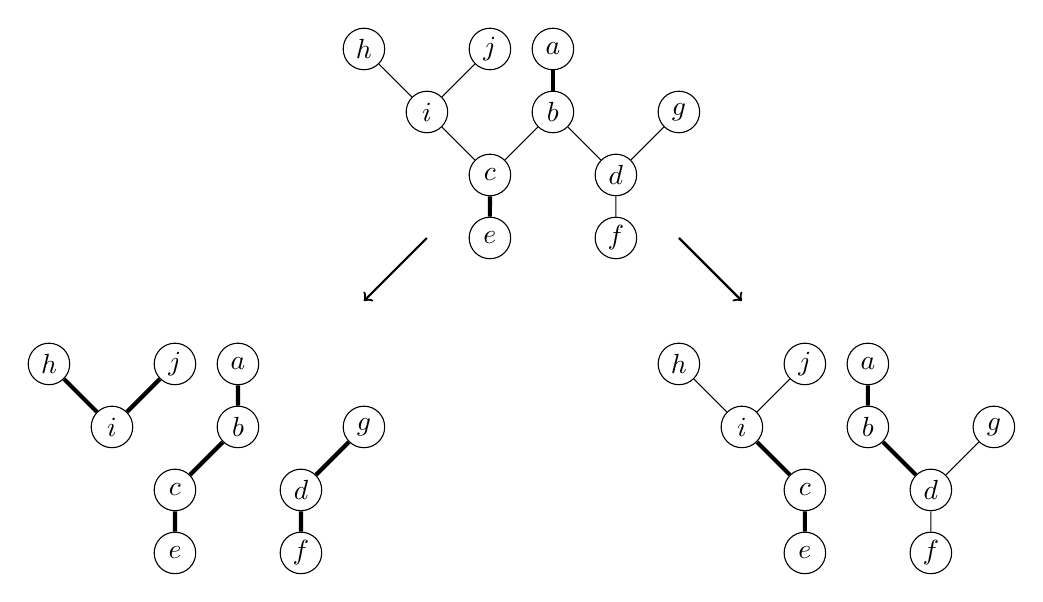
\begin{tikzpicture}[scale=0.8]
\tikzstyle{vertex}=[draw,shape=circle,inner sep=0pt,minimum size=15pt]
\path (0,0) node[vertex](f0){$a$};
\path (-2,-1) node[vertex](x0){$i$} (-1,-2) node[vertex](x1){$c$} (0,-1) node[vertex](f1){$b$} (1,-2) node[vertex](y1){$d$} (2,-1) node[vertex](y0){$g$};
\path (-1,-3) node[vertex](x2){$e$} (1,-3) node[vertex](y2){$f$};
\path (-3,0) node[vertex](x3){$h$} (-1,0) node[vertex](x4){$j$};
\draw[line width=1.5pt] (f0) -- (f1);
\draw[line width=1.5pt] (x2) -- (x1);
\draw (x0) -- (x1) -- (f1) -- (y1) -- (y2);
\draw (x3) -- (x0) -- (x4);
\draw (y0) -- (y1);

\path (-5,-5) node[vertex](f0){$a$};
\path (-7,-6) node[vertex](x0){$i$} (-6,-7) node[vertex](x1){$c$} (-5,-6) node[vertex](f1){$b$} (-4,-7) node[vertex](y1){$d$} (-3,-6) node[vertex](y0){$g$};
\path (-6,-8) node[vertex](x2){$e$} (-4,-8) node[vertex](y2){$f$};
\path (-8,-5) node[vertex](x3){$h$} (-6,-5) node[vertex](x4){$j$};
\draw[line width=1.5pt] (f0) -- (f1) -- (x1) -- (x2);
\draw[line width=1.5pt] (x3) -- (x0) -- (x4);
\draw[line width=1.5pt] (y2) -- (y1) -- (y0);

\path (5,-5) node[vertex](f0){$a$};
\path (3,-6) node[vertex](x0){$i$} (4,-7) node[vertex](x1){$c$} (5,-6) node[vertex](f1){$b$} (6,-7) node[vertex](y1){$d$} (7,-6) node[vertex](y0){$g$};
\path (4,-8) node[vertex](x2){$e$} (6,-8) node[vertex](y2){$f$};
\path (2,-5) node[vertex](x3){$h$} (4,-5) node[vertex](x4){$j$};
\draw[line width=1.5pt] (f0) -- (f1) -- (y1);
\draw[line width=1.5pt] (x0) -- (x1) -- (x2);
\draw (x3) -- (x0) -- (x4);
\draw (y0) -- (y1) -- (y2);

\draw[thick, ->] (-2,-3) -- (-3,-4);
\draw[thick, ->] (2,-3) -- (3,-4);
\end{tikzpicture}
\end{center}
\caption[An instance of the recursive step in Eppstein's algorithm]{An instance of the recursive step in Eppstein's backtracking algorithm for the TSP~\cite{eppstein2007} for a subgraph of a larger graph $G$, with forced edges displayed in bold and  branching on edge $bc$. If we force $bc$, then $b$ and $c$ are both incident to two forced edges, so $bd$ and $ci$ cannot be part of the Hamiltonian cycle and can be removed from the graph. After these edges are removed, vertices $i$ and $d$ are both of degree $2$, so in order to reach those vertices the edges $hi$, $ij$, $df$ and $dg$ must also be included in the Hamiltonian cycle. So forcing $bc$ has overall added five edges to the Hamiltonian cycle. On the other hand, if we remove edge $bc$, we find that $b$ and $c$ are vertices of degree $2$, so edges $bd$ and $ci$ must be part of the Hamiltonian cycle. Thus we have only added two more edges to the Hamiltonian cycle.
\label{fig:size-decrease-by-two}}
\end{figure}

% ------------------------------------------------------------------------------

\section{Quantum speedups for the Travelling Salesman Problem on bounded-degree graphs \label{sec:bd}}
\label{sec:deg3}

Our algorithms are based on applying the quantum algorithm for backtracking (Theorem \ref{thm:backtrack}) to Xiao and Nagamochi's algorithm for solving the TSP for degree-3 graphs~\cite{xiao2016degree3}. Before describing our algorithms, we need to introduce some terminology from~\cite{xiao2016degree3} and describe their original algorithm. The algorithm, and its analysis, are somewhat involved, so we omit details wherever possible.

\subsection{The algorithm of Xiao and Nagamochi}
\label{sec:xndeg3}

A graph $G$ is $k$-edge connected if there are $k$ edge-disjoint paths between every pair of vertices. An edge in $G$ is said to be forced if it must be included in the final tour, and unforced otherwise. The set of forced edges is denoted $F$, and the set of unforced edges is denoted $U$. An induced subgraph of unforced edges which is maximal and connected is called a $U$-component. If a $U$-component is just a single vertex, then that $U$-component is trivial. A maximal sequence $\mathcal{C}$ of edges in a $U$-component $H$ is called a circuit if either:
%
\begin{itemize}
\item $\mathcal{C} = \{xy\}$ and there are three edge-disjoint paths from $x$ to $y$,
\item or $\mathcal{C} = \{c_0, c_1,\dots,c_{m-1}\}$ such that for $0 \leq i < m-1$, there is a subgraph $B_i$ of $H$ such that the only two unforced edges incident to $B_i$ are $c_i$ and $c_{i+1}$.
\end{itemize}
%

A circuit is reducible if subgraph $B_i$ for some $i$ is incident to only two edges. In order for $B_i$ to be reached, both edges incident to $B_i$ need to be forced. Forcing one edge in the circuit then means that the other edges can be either forced or removed. The polynomial time and space process by Xiao and Nagamochi to reduce circuits, by forcing and removing alternating edges in the circuit, is known as the {\em circuit procedure} \cite{xiao2016degree3}.

Note that each edge can be in at most one circuit. If two distinct circuits $\mathcal{C}, \mathcal{C}'$ shared an edge $e_i$, then there are two possibilities. The first is that there is a subgraph $B_i$ incident to unforced edges $e_i \in \mathcal{C} \cap \mathcal{C}', e_{i+1} \in \mathcal{C} - \mathcal{C}', e_j \in \mathcal{C}' - \mathcal{C}$. In this case, $B_i$ is incident to more than two unforced edges, so neither $\mathcal{C}$ nor $\mathcal{C}'$ are circuits, which is a contradiction.

The second is that there is some edge $e_i$ which is incident to distinct subgraphs $B_i, B_i'$ related to $\mathcal{C}, \mathcal{C}'$, respectively. Circuits are maximal sequences, so it cannot be the case that $B_i$ is a subgraph of $B_i'$, otherwise $\mathcal{C}' \subseteq \mathcal{C}$. Now we consider the subgraphs $B_i \cap B_i'$ and $B_i - B_i'$, which must be connected by unforced edges as they are both subgraphs of $B_i$. These unforced edges are incident to $B_i'$, which is a contradiction as they are not part of $\mathcal{C}'$.

Let $X$ be a subgraph. We define $\text{cut}(X)$ to be the set of edges that connect $X$ to the rest of the graph. If $|\text{cut}(X)| = 3$, then we say that $X$ is $3$-cut reducible. It was shown by Xiao and Nagamochi~\cite{xiao2016degree3} that, if $X$ is 3-cut reducible, $X$ can be replaced with a single vertex of degree $3$ with outgoing edges weighted such that the length of the shortest Hamiltonian cycle is preserved.

The definition of $4$-cut reducible is more complex. Let $X$ be a subgraph such that $\text{cut}(X) \subseteq F$ and $|\text{cut}(X)| = 4$. A solution to the TSP would have to partition $X$ into two disjoint paths such that every vertex in $X$ is in one of the two paths. If $x_1, x_2, x_3$ and $x_4$ are the four vertices in $X$ incident to the four edges in $\text{cut}(X)$, then there are three ways these paths could start and end:
%
\begin{itemize}
\item $x_1 \leftrightarrow x_2$ and $x_3 \leftrightarrow x_4$,
\item $x_1 \leftrightarrow x_3$ and $x_2 \leftrightarrow x_4$,
\item or $x_1 \leftrightarrow x_4$ and $x_2 \leftrightarrow x_3$.
\end{itemize}
%
We say that $X$ is $4$-cut reducible if, for at least one of these cases, it is impossible to create two disjoint paths in $X$ that include all vertices in $X$. Xiao and Nagamochi defined a polynomial time and space process for applying the above reductions, known as {\em $3/4$-cut reduction}~\cite{xiao2016degree3}.

A set of edges $\{e_i\}$ are {\em parallel} if they are incident to the same vertices (note that here we implicitly let $G$ be a multigraph; these may be produced in intermediate steps of the algorithm). If there are only two vertices in the graph, then the TSP can be solved directly by forcing the shortest two edges. Otherwise if at least one of the edges is not forced, then we can reduce the problem by removing the longer unforced edges until the vertices are only adjacent via one edge. This is the process Xiao and Nagamochi refer to as {\em eliminating parallel edges} \cite{xiao2016degree3}.

Finally, a graph is said to satisfy the parity condition if every $U$-component is incident to an even number of forced edges and for every circuit $\mathcal{C}$, an even number of the corresponding subgraphs $B_i$ satisfy that $|\text{cut}(B_i) \cap F|$ is odd.

%We will now explain how to speed up Xiao and Nagamochi's algorithm for graphs of bounded degree $3$. We shall start by proving the following lemma:

%\begin{lemma}
%Let $G$ be a graph of bounded degree $3$. There is a quantum algorithm which finds a Hamiltonian cycle in $G$ with probability $\delta$ in $O(2^{3n/20}\poly(n)\log(1/\delta))$.
%\label{thm:hamiltonian-cycle}
%\end{lemma}

%It is worth noting that Lemma \ref{thm:hamiltonian-cycle} beats the algorithm by Mandr{\`a}, Guerreschi and Aspuru-Guzik for finding a Hamiltonian cycle \cite{mandra2016}, which for bounded degree $3$ graphs runs in time $O(2^{n/4})$.

We are now ready to describe Xiao and Nagamochi's algorithm. The algorithm takes as input a graph $G = (V, E)$ and a set of forced edges $F \subseteq E$ and returns the length of the shortest Hamiltonian cycle in $G$ containing all the edges in $F$, if one exists.

The algorithm is based on four subroutines: {\em eliminating parallel edges}, the {\em 3/4-cut reduction}, {\em selecting a good circuit} and the {\em circuit procedure}, as well as the following lemma.

\begin{lemma}[Eppstein~\cite{eppstein2007}]
\label{lem:trivial}
If every $U$-component in a graph $G$ is trivial or a component of a 4-cycle, then a minimum cost tour can be found in polynomial time.
\end{lemma}

We will not define the subroutines here in any detail; for our purposes, it is sufficient to assume that they all run in polynomial time and space. The circuit procedure for a circuit $\mathcal{C}$ begins by either adding an edge $e \in \mathcal{C}$ to $F$ or deleting it from the graph, then performing some other operations. ``Branching on a circuit $\mathcal{C}$ at edge $e \in \mathcal{C}$'' means generating two new instances from the current instance by applying each of these two variants of the circuit procedure starting with $e$.

The Xiao-Nagamochi algorithm is described in Algorithm \ref{alg:tsp3}, reproduced from~\cite{xiao2016degree3}. Lines 2 and 3 check that the existence of a Hamiltonian cycle is not ruled out, by ensuring that that there are at least two disjoint paths between any pair of vertices and that the graph satisfies the parity condition. Lines 4 and 5 reduce any reducible circuit by initially forcing one edge and then alternately removing and forcing edges. Lines 6 \& 7 remove any parallel edges from the graph, and lines 8 \& 9 remove any circuits of three edges as well as setting up circuits of four edges so that all edges incident to them are forced. Lines 10-12 are the recursive step, branching on a good circuit by either forcing or removing an edge in the circuit and then applying the circuit procedure. The algorithm continues these recursive calls until it either finds a Hamiltonian cycle or $G \setminus F$ is a collection of single vertices and cycles of length $4$, all of which are disjoint from one another, at which point the problem can be solved in polynomial time via lines 14 and 15.

\begin{algorithm}
\Fn{\FnTSPthree{$G$, $F$}}{
\KwIn{A graph $G=(V,E)$, a set of forced edges $F\subseteq E$}
\KwOut{The length of the shortest Hamiltonian cycle which includes all edges in $F$}
\uIf{$G$ is not $2$-edge-connected or the instance violates the parity condition}{
Return $\infty$\;
}\uElseIf{there is a reducible circuit $\mathcal{C}$}{
Return \FnTSPthree{$G'$, $F'$} for an instance $(G',F')$ obtained by applying the circuit procedure on $\mathcal{C}$ started by adding a reducible edge in $\mathcal{C}$ to $F$\;
}\uElseIf{there is a pair of parallel edges}{
Return \FnTSPthree{$G'$, $F'$} for an instance $(G',F')$ obtained by applying the reduction rule of eliminating parallel edges\;
}\uElseIf{there is a $3/4$-cut reducible subgraph $X$ containing at most eight vertices}{
Return \FnTSPthree{$G'$, $F'$} for an instance $(G',F')$ obtained by applying the $3/4$-cut reduction on $X$\;
}\uElseIf{there is a $U$-component $H$ that is neither trivial nor a $4$-cycle}{
Select a good circuit $\mathcal{C}$ in $H$\;
Return $\min\{$\FnTSPthree{$G_1$, $F_1$}$,$ \FnTSPthree{$G_2$, $F_2$}$\}$, where $(G_1,F_1)$ and $(G_2,F_2)$ are the
two resulting instances after branching on $\mathcal{C}$\;
}\Else{\tcc{each $U$-component of the graph is trivial or a $4$-cycle}
Solve the problem directly in polynomial time by Lemma \ref{lem:trivial}\;
Return the cost of an optimal tour\;
}
}
\caption{\label{alg:tsp3} The Xiao-Nagamochi algorithm for solving the TSP on degree-3 graphs.}
\end{algorithm}

Xiao and Nagamochi looked at how the steps of the algorithm, and in particular the branching step, reduced the size of the problem for different graph structures. From this they derived a quasiconvex program corresponding to $19$ branching vectors, each describing how the problem size is reduced at the branching step in different circumstances. Analysis of this quasiconvex program showed that the algorithm runs in $O^*(2^{3n/10}\log L)$ time and polynomial space \cite{xiao2016degree3}.

\subsection{Quantum speedup of the Xiao-Nagamochi algorithm}
\label{sec:deg3speedup}

Here we describe how we apply the quantum backtracking algorithm to the Xiao-Nagamochi algorithm. It is worth noting that the quantum backtracking algorithm will not necessarily return the shortest Hamiltonian cycle, but instead returns a randomly selected Hamiltonian cycle that it found. Adding constraints on the length of the Hamiltonian cycles to our predicate and running the quantum backtracking algorithm multiple times will allow us to find a solution to the TSP.

The first step towards applying the quantum backtracking algorithm is to define the set of partial assignments. A partial assignment will be a list of edges in $G$ ordered by when they are assigned in the backtracking algorithm and paired with whether the assignment was to force or remove the edge. The assignment is denoted $A \in (\{1,\dots,m\}, \{\text{force}, \text{remove}\})^j$, where $j \leq m$. We have $m \le 3n/2$ as $G$ is degree-3.

%The quantum approach to backtracking requires us to define a predicate $P$ and heuristic $h$, each taking as input a partial assignment. The variables we assign in the backtracking algorithm correspond to the edges of the graph, of which there are at most $3n/2$ for a degree-3 graph. Each variable represents our decision to include or exclude the corresponding edge from the tour.

The quantum approach to backtracking requires us to define a predicate \FnPredicatethree and heuristic \FnHeuristicthree, described by Algorithms \ref{alg:predicate} and \ref{alg:heuristic}, respectively, and each taking as input a partial assignment. Our predicate and heuristic make use of a reduction function, introduced in \cite{xiao2016degree3}, as a subroutine; this function is denoted \FnReductionthree and described as Algorithm \ref{alg:reduction} in Section \ref{sec:reduction}. However it may be worth noting that the algorithm uses the original graph $G$, and partial assignments of it at each stage.

Firstly, we describe the predicate in Algorithm \ref{alg:predicate}. Lines 3 \& 4 match lines 2 and 3 of Xiao and Nagamochi's algorithm. Lines 5 and 6 are where the same conditions are met as in lines 14 and 15 of Xiao and Nagamochi's algorithm, where a shortest length Hamiltonian cycle is guaranteed to exist and can be found in polynomial time classically via Lemma \ref{lem:trivial}. The rest of Algorithm \ref{alg:predicate} continues the branching process, which together with how the circuit is picked by \FnHeuristicthree and the use of the circuit procedure in \FnReductionthree matches the branching step of Xiao and Nagamochi.

\begin{algorithm}
\Fn{\FnPredicatethree{$A$}}{
\KwIn{A partial assignment $A = ((e_1, A_1),\dots,(e_j, A_j))$ describing edges that have been forced or removed}
\KwOut{True, false, or indeterminate depending on if a Hamiltonian cycle can be found}
Using the partial assignment $A$, run \FnReductionthree{$G$, $F$} to get $(G', F')$\;
\uIf{$G$ is not $2$-edge-connected or fails the parity condition}{
Return false\;
}\uElseIf{Every $U$-component in $G'$ is either trivial or a $4$-cycle}{
Return true\;
}\Else{
Return indeterminate\;
}
}
\caption{\label{alg:predicate} The predicate function for the Xiao-Nagamochi algorithm for degree-3 graphs.}
\end{algorithm}

The heuristic is described in Algorithm \ref{alg:heuristic}, taking as input a partial assignment $A = ((e_1, A_1),\dots,(e_j, A_j))$ of the edges of $G$. Here we apply the same branching strategy as Xiao and Nagamochi's algorithm, by selecting the next circuit to branch on and picking an edge in that circuit. If the reduced version of the graph results in \FnHeuristicthree picking an edge corresponding to multiple edges in the original graph, line 4 ensures that we only return one of these edges to the backtracking algorithm, as the reduction function will ensure that every edge in the original graph corresponding to an edge in the reduced graph will be consistently forced or removed. The rest of the circuit will be forced or removed by line 26 of the reduction function (Algorithm \ref{alg:reduction}).

\begin{algorithm}
\Fn{\FnHeuristicthree{$A$}}{
\KwIn{A partial assignment $A = ((e_1, A_1),\dots,(e_j, A_j))$ describing edges that have been forced or removed}
\KwOut{The next edge to force or remove from $G$}
Using the partial assignment $A$, run \FnReductionthree{$G$, $F$} to get $(G', F')$\;
Select a $U$-component in $G'$ that is neither trivial nor a cycle of length $4$. Select a circuit $\mathcal{C}$ in that component that fits the criteria of a ``good'' circuit~\cite{xiao2016degree3}, then select an edge $e_i' \in \mathcal{C}$\;
Return an edge in $G$ corresponding to $e_i'$ \;
\tcc{if there is more than one edge corresponding to $e_i'$, we can choose one arbitrarily}
}
\caption{\label{alg:heuristic} The heuristic function for the Xiao-Nagamochi algorithm for degree-3 graphs.}
\end{algorithm}

We can now apply the backtracking algorithm (Theorem \ref{thm:backtrack}) to \FnPredicatethree and \FnHeuristicthree to find a Hamiltonian cycle. We will later choose its failure probability $\delta$ to be sufficiently small that we can assume that it always succeeds, i.e.\ finds a Hamiltonian cycle if one exists, and otherwise reports that one does not exist. At the end of the algorithm, we will receive either the information that no assignment was found, or a partial assignment. By applying the reduction steps and the partial assignments, we can reconstruct the graph at the moment our quantum algorithm terminated, which will give a graph such that every $U$-component is either trivial or a 4-cycle. We then construct and return the full Hamiltonian cycle in polynomial time using step $6$ of Xiao and Nagamochi's algorithm~\cite{xiao2016degree3}. %In order to reduce the probability of not returning a Hamiltonian cycle when one does exist, we repeat the algorithm multiple times and either return the shortest Hamiltonian cycle found or report that no Hamiltonian cycle was found.

To solve the TSP, we need to find the shortest Hamiltonian cycle. This can be done as follows. First, we run the backtracking algorithm. If the backtracking algorithm does not return a Hamiltonian cycle then we report that no Hamiltonian cycle was found. Otherwise after receiving Hamiltonian cycle $\Gamma$ with length $L_\Gamma$, we create variables $\ell \leftarrow 0$ \& $u \leftarrow L_\Gamma$ and modify the predicate to return false if
%
\begin{equation}
\sum_{e_{i,j}\in F}c_{ij} \geq \lceil(\ell + u)/2\rceil.
\end{equation}
%
If no cycle is found after running the algorithm again, we set $\ell \leftarrow \lceil(\ell + u)/2\rceil$ and repeat. Otherwise, upon receiving Hamiltonian cycle $\Gamma'$ with total cost $L_{\Gamma'}$, we set $u \leftarrow L_{\Gamma'}$ and repeat. We continue repeating until $\ell$ and $u$ converge, at which point we return the Hamiltonian cycle found by the algorithm. The scenario that will give the longest runtime is when the shortest cycle is found during the first run of the backtracking algorithm: the backtracking algorithm will fail to find a Hamiltonian cycle shorter than $\lceil(\ell + u)/2\rceil$, update $\ell$ and repeat until $\ell$ and $u$ converge. In this case, this algorithm matches a binary search. So the number of repetitions of the backtracking algorithm required to return the shortest Hamiltonian cycle is at most $O(\log L')$, where
%
%We can find the shortest Hamiltonian cycle by repeating the algorithm at most $O(\log L')$ times, where
%
\begin{align}
L' = \sum_{i = 1}^{n}\max \{c_{ij} : j \in \{1,\dots,n\} \}
\label{eqn:l}
\end{align}
%
is an upper bound on the total cost of any Hamiltonian cycle in the graph.

\subsection{The reduction function}
\label{sec:reduction}

Finally, we describe the reduction function, which takes the original graph $G$ and partial assignment $A$, and applies the partial assignment to this graph in order to reduce it to a smaller graph $G'$ with forced edges $F'$. This reduction might mean that forcing or removing a single edge in $G'$ would be akin to forcing several edges in $G$. For example, let $X$ be a $3$-reducible subgraph of at most $8$ vertices with $\text{cut}(X) = \{ax_1, bx_2, cx_3\}$ for vertices $x_1, x_2, x_3 \in V(X)$. The $3/4$-cut reduction reduces $X$ to a single vertex $x \in G'$ with edges $ax, bx, cx$. If the edges $ax$ and $bx$ are forced, this is equivalent to forcing every edge in $\Pi \cup \{ax_1, bx_2\}$, where $\Pi$ is the shortest path that starts at $x_1$, visits every vertex in $X$ exactly once, and ends at $x_2$. As we need to solve the problem in terms of the overall graph $G$ and not the reduced graph $G'$, our assigned variables need to correspond to edges in $G$. To do this, our \FnHeuristicthree function described in Sec.\ \ref{sec:deg3speedup} includes a step where if the edge selected in $G'$ corresponds to multiple edges in $G$, we simply select one of the corresponding edges in $G$ to return. Likewise, if the next edge in our partial assignment is one of several edges in $G$ corresponding to a single edge in $G'$, we apply the same assignment to all of the other corresponding edges in $G$.

The reduction function is described in Algorithm \ref{alg:reduction}, using reductions and procedures from Xiao and Nagamochi \cite{xiao2016degree3}. This function applies the edge assignments made so far, as well as any possible reductions at each step. Lines 5 and 6 case recreate lines 4 and 5 from Xiao and Nagamochi's original algorithm by applying the circuit procedure where possible. Steps 7 and 8 recreate steps 6 and 7 of the original algorithm by applying the reduction of parallel edges. And steps 9 \& 10 case recreate steps 8 and 9 of the original algorithm via the $3/4$-cut reduction. We then apply the next step of the branching that has been performed so far, to ensure that the order in which the edges are forced is the same as in the classical algorithm, followed by branching on a circuit at edge $e_i$ via the circuit procedure. Finally, we check whether or not the graph can be reduced further by running the reduction steps again for edge $j$.

\begin{algorithm}
\Fn{\FnReductionthree{$G$, $F$}}{
\KwIn{A graph $G=(V,E)$, a partial assignment of edges $A$}
\KwOut{A reduced graph $G'$ and set of forced edges $F'$}
Create a copy of the graph $G' \leftarrow G$ and set of forced edges $F' \leftarrow \emptyset$\;
\For{$i=1,\dots,j$}{
\Repeat{None of the cases apply}{
\uIf{$G'$ contains a reducible circuit $\mathcal{C}$}{
Apply the circuit procedure to $\mathcal{C}$\;
}\uElseIf{$G'$ contains parallel edges}{
Apply the reduction rule of eliminating parallel edges\;
}\ElseIf{$G'$ contains a subgraph $X$ of at most $8$ vertices such that $X$ is $3/4$-cut reducible}{
Apply the $3$/$4$-cut reduction to $X$\;
}
}
\uIf{$A_i = \text{force}$}{
\uIf{$e_i$ is in a set of edges corresponding to a single reduced edge in $e_i' \in G'$}{
$F' \leftarrow F' \cup \{e_i'\}$\;
}\Else{
$F' \leftarrow F' \cup \{e_i\}$\;
}
}\Else{\tcc{$A_i = \text{remove}$}
\uIf{$e_i$ is in a set of edges corresponding to a single reduced edge in $e_i' \in G'$}{
$G' \leftarrow G' - \{e_i'\}$\;
}\Else{
$G' \leftarrow G' - \{e_i\}$\;
}
}
Apply the circuit procedure to the rest of the circuit containing edge $e_i$\;
}
Repeat lines 4-12 until no further reductions can be applied\;
Return $(G', F')$\;
}
\caption{\label{alg:reduction} The reduction function for degree-3 graphs.}
\end{algorithm}

One might ask if an edge could be part of two circuits, in which case our algorithm would fail as it would not be able to reduce the circuit. However, as discussed in Sec.\ \ref{sec:xndeg3}, any edge can only be part of at most one circuit.

\subsection{Analysis}

All procedures in the reduction algorithm can be completed in polynomial time in $n$ and $\log L$~\cite{xiao2016degree3}. All of these steps also reduce the size of a problem by at least a constant amount, so only a polynomial number of these steps are needed. Step 2(b) is constant time and step 2(c) can be run in polynomial time as the circuit is now reducible. All steps are only repeated $O(m)$ times, so the whole reduction algorithm runs in polynomial time in terms of $m$.

The remaining steps in the heuristic subroutine run in polynomial time as searching for a good circuit in a component can be done in polynomial time \cite{xiao2016degree3}. Likewise, remaining steps in the predicate function involve looking for certain structures in the graph that can be found in polynomial time. As a result, the runtimes for the \FnPredicatethree and \FnHeuristicthree functions are both polynomial in $m$.

By Theorem \ref{thm:backtrack}, the number of calls to \FnPredicatethree and \FnHeuristicthree we make in order to find a Hamiltonian cycle with failure probability $\delta$ is $O(\sqrt{T}\poly(m)\log (1/\delta))$, where $T$ is the size of the backtracking tree, which in our case is equal to the number of times the Xiao-Nagamochi algorithm branches on a circuit. \FnPredicatethree and \FnHeuristicthree both run in polynomial time and as a result can be included in the $\poly(m)$ term of the runtime. Because $m \leq 3n/2$, the polynomial term in this bound is also polynomial in terms of $n$.

The behaviour of the \FnPredicatethree and \FnHeuristicthree subroutines is designed to reproduce the behaviour of Xiao and Nagamochi's TSP3 algorithm~\cite{xiao2016degree3}. It is shown in~\cite[Theorem 1]{xiao2016degree3} that this algorithm is correct, runs in time $O^*(2^{3n/10})$ and uses polynomial space. As the runtime of the TSP3 algorithm is an upper bound on the number of branching steps it makes, the algorithm branches on a circuit $O^*(2^{3n/10})$ times. Therefore, the quantum backtracking algorithm finds a Hamiltonian cycle, if one exists, with failure probability at most $\delta$ in time $O^*(2^{3n/20}\log L \log(1/\delta)) \approx O^*(1.110^n\log L \log(1/\delta))$ and polynomial space.

Finding the shortest Hamiltonian cycle requires repeating the algorithm $O(\log L')$ times, where $L'$ is given in Equation \ref{eqn:l}. By using a union bound over all the runs of the algorithm, to ensure that all runs succeed with high probability it is sufficient for the failure probability $\delta$ of each run to be at most $O(1/(\log L'))$. From this we obtain the following result, proving the first part of Theorem \ref{thm:deg34}:

\begin{theorem}
There is a bounded-error quantum algorithm which solves the TSP on degree-3 graphs in time $O^*(1.110^n \log^2 L \log \log L)$, where $L$ is the maximum edge cost. The algorithm uses $\poly(n)$ space.
\end{theorem}

Note that we have used the bound $L' \le n L$, where the extra factor of $n$ is simply absorbed into the hidden $\poly(n)$ suppression.

\section{Extending to higher-degree graphs \label{sec:higher-bound}}

We next consider degree-$k$ graphs for $k \ge 4$. We start with degree-4 graphs by applying the quantum backtracking algorithm to another algorithm by Xiao and Nagamochi~\cite{xiao2016degree4}. We then extend this approach to graphs of higher degree by reducing the problem to degree-4 graphs.

\subsection{Degree-4 graphs}

Here we will show the following, which is the second part of Theorem \ref{thm:deg34}:

\begin{theorem}
There is a bounded-error quantum algorithm which solves the TSP for degree-4 graphs in time $O^*(1.301^n\log^2 L \log \log L)$, where $L$ is the maximum edge cost. The algorithm uses $\poly(n)$ space.
\end{theorem}

As the argument is very similar to the degree-3 case, we only sketch the proof.

\begin{proof}[Proof sketch]
Xiao and Nagamochi's algorithm for degree-4 graphs works in a similar way to their algorithm for degree-3 graphs. Indeed, the predicate function considers largely the same cases as in Algorithm \ref{alg:predicate}:

\begin{lemma}[Xiao and Nagamochi \cite{xiao2016degree4}]Let $G=(V,E)$ be a graph and $F\subseteq E$ a set of forced edges. There is no Hamiltonian cycle that visits every edge in $F$ if:

\begin{enumerate}
\item $G$ is not 2-edge-connected;
\item a vertex $v$ is incident to more than 2 edges in $F$;
\item $(V, F)$ contains a non-Hamiltonian cycle;
\item or there exists a $U$-component incident to an odd number of edges in $F$.
\end{enumerate}
\end{lemma}

Cases 1 and 4 are already considered in Algorithm \ref{alg:predicate}, with case $4$ forming part of the parity condition. The algorithm also only returns an definite solution in the same way as the degree $3$ case, via Lemma \ref{lem:trivial}. As a result, our new predicate only needs to care about cases $2$ and $3$, both of which can be checked in polynomial time.

The reductions utilised are also simple to observe and related to those used in Algorithm \ref{alg:reduction}. The first two are removing unforced edges incident to any vertex $v$ where $v$ is incident to two forced edges, and forcing any edges incident to a vertex of degree 2, both of which are similar to what is already performed by the circuit procedure. Likewise, the fourth reduction process is reducing triangles in the graph to a single vertex, akin to the 3-cut reduction from before.

The third reduction process is more involved, but can still be computed in polynomial time. This reduction checks for each edge $e$ if it is a bridge, an edge that would split a $U$-component $H$ in the graph into two disconnected subgraphs $H_1$ and $H_2$. If $e$ is a bridge, then it is either forced or removed depending on if $H_1$ is incident to and odd or even number of forced edges, respectfully. If $H$ is incident to an even number of forced edges, then so are the subgraphs $H_1$ and $H_2$. Note that this might leave $H_2$ disconnected from the rest of the graph, but this would violate the 2-edge-connected rule and therefore be rejected by the predicate.

The heuristic is more involved than previously, but essentially consists of selecting a degree-4 vertex $v$ incident to a forced edge and branching on an edge incident to that vertex. If no such vertex exists then we select a degree-3 vertex $v$ incident to a forced edge and branch on an edge incident to a vertex at most two edges away from $v$. We shall omit details on how the branching edge is chosen for simplicity, but note that these conditions can be computed in polynomial time.

We apply the quantum backtracking algorithm as before, finding a Hamiltonian cycle with failure probability $\delta$ in $O^*(1.301^n\log L\log(1/\delta))$ time. We then use binary search to find the shortest Hamiltonian cycle after $O(\log L)$ repetitions of the algorithm, rejecting if the total length of the forced edges is above a given threshold. To achieve overall failure probability $1/3$, the algorithm runs in $O^*(1.301^n\log^2 L\log \log L)$ time.
\end{proof}

\subsection{Degree-5 and degree-6 graphs}

\begin{figure}
\begin{center}
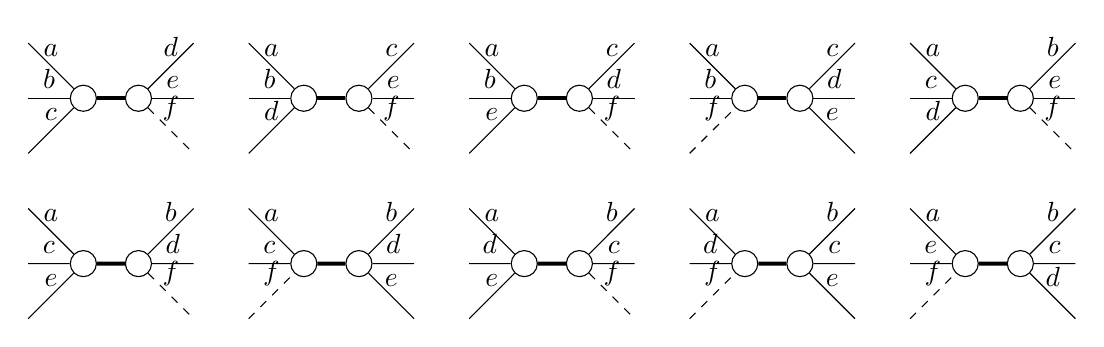
\begin{tikzpicture}[scale=0.7]
\tikzstyle{vertex}=[draw,shape=circle]
\path (0,0) node[vertex](x1){} (1,0) node[vertex](y1){};
\draw[line width=1.5pt] (x1) -- (y1);
\draw[] (-1,1) -- node[above] {$a$} (x1);
\draw[] (-1,0) -- node[above] {$b$} (x1);
\draw[] (-1,-1) -- node[above] {$c$} (x1);
\draw[] (y1) -- node[above] {$d$} (2,1);
\draw[] (y1) -- node[above] {$e$} (2,0);
\draw[dashed] (y1) -- node[above] {$f$} (2,-1);

\path (4,0) node[vertex](x1){} (5,0) node[vertex](y1){};
\draw[line width=1.5pt] (x1) -- (y1);
\draw[] (3,1) -- node[above] {$a$} (x1);
\draw[] (3,0) -- node[above] {$b$} (x1);
\draw[] (3,-1) -- node[above] {$d$} (x1);
\draw[] (y1) -- node[above] {$c$} (6,1);
\draw[] (y1) -- node[above] {$e$} (6,0);
\draw[dashed] (y1) -- node[above] {$f$} (6,-1);

\path (8,0) node[vertex](x1){} (9,0) node[vertex](y1){};
\draw[line width=1.5pt] (x1) -- (y1);
\draw[] (7,1) -- node[above] {$a$} (x1);
\draw[] (7,0) -- node[above] {$b$} (x1);
\draw[] (7,-1) -- node[above] {$e$} (x1);
\draw[] (y1) -- node[above] {$c$} (10,1);
\draw[] (y1) -- node[above] {$d$} (10,0);
\draw[dashed] (y1) -- node[above] {$f$} (10,-1);

\path (12,0) node[vertex](x1){} (13,0) node[vertex](y1){};
\draw[line width=1.5pt] (x1) -- (y1);
\draw[] (11,1) -- node[above] {$a$} (x1);
\draw[] (11,0) -- node[above] {$b$} (x1);
\draw[dashed] (11,-1) -- node[above] {$f$} (x1);
\draw[] (y1) -- node[above] {$c$} (14,1);
\draw[] (y1) -- node[above] {$d$} (14,0);
\draw[] (y1) -- node[above] {$e$} (14,-1);

\path (16,0) node[vertex](x1){} (17,0) node[vertex](y1){};
\draw[line width=1.5pt] (x1) -- (y1);
\draw[] (15,1) -- node[above] {$a$} (x1);
\draw[] (15,0) -- node[above] {$c$} (x1);
\draw[] (15,-1) -- node[above] {$d$} (x1);
\draw[] (y1) -- node[above] {$b$} (18,1);
\draw[] (y1) -- node[above] {$e$} (18,0);
\draw[dashed] (y1) -- node[above] {$f$} (18,-1);

\path (0,-3) node[vertex](x1){} (1,-3) node[vertex](y1){};
\draw[line width=1.5pt] (x1) -- (y1);
\draw[] (-1,-2) -- node[above] {$a$} (x1);
\draw[] (-1,-3) -- node[above] {$c$} (x1);
\draw[] (-1,-4) -- node[above] {$e$} (x1);
\draw[] (y1) -- node[above] {$b$} (2,-2);
\draw[] (y1) -- node[above] {$d$} (2,-3);
\draw[dashed] (y1) -- node[above] {$f$} (2,-4);

\path (4,-3) node[vertex](x1){} (5,-3) node[vertex](y1){};
\draw[line width=1.5pt] (x1) -- (y1);
\draw[] (3,-2) -- node[above] {$a$} (x1);
\draw[] (3,-3) -- node[above] {$c$} (x1);
\draw[dashed] (3,-4) -- node[above] {$f$} (x1);
\draw[] (y1) -- node[above] {$b$} (6,-2);
\draw[] (y1) -- node[above] {$d$} (6,-3);
\draw[] (y1) -- node[above] {$e$} (6,-4);

\path (8,-3) node[vertex](x1){} (9,-3) node[vertex](y1){};
\draw[line width=1.5pt] (x1) -- (y1);
\draw[] (7,-2) -- node[above] {$a$} (x1);
\draw[] (7,-3) -- node[above] {$d$} (x1);
\draw[] (7,-4) -- node[above] {$e$} (x1);
\draw[] (y1) -- node[above] {$b$} (10,-2);
\draw[] (y1) -- node[above] {$c$} (10,-3);
\draw[dashed] (y1) -- node[above] {$f$} (10,-4);

\path (12,-3) node[vertex](x1){} (13,-3) node[vertex](y1){};
\draw[line width=1.5pt] (x1) -- (y1);
\draw[] (11,-2) -- node[above] {$a$} (x1);
\draw[] (11,-3) -- node[above] {$d$} (x1);
\draw[dashed] (11,-4) -- node[above] {$f$} (x1);
\draw[] (y1) -- node[above] {$b$} (14,-2);
\draw[] (y1) -- node[above] {$c$} (14,-3);
\draw[] (y1) -- node[above] {$e$} (14,-4);

\path (16,-3) node[vertex](x1){} (17,-3) node[vertex](y1){};
\draw[line width=1.5pt] (x1) -- (y1);
\draw[] (15,-2) -- node[above] {$a$} (x1);
\draw[] (15,-3) -- node[above] {$e$} (x1);
\draw[dashed] (15,-4) -- node[above] {$f$} (x1);
\draw[] (y1) -- node[above] {$b$} (18,-2);
\draw[] (y1) -- node[above] {$c$} (18,-3);
\draw[] (y1) -- node[above] {$d$} (18,-4);
\end{tikzpicture}
\end{center}
\caption[Breaking a vertex of degree 5 or 6 into two lower-degree vertices]{Breaking a vertex of degree 5 or 6 into two lower-degree vertices. In the degree-5 case, dashed edge $f$ is not present and the vertex is split into one vertex of degree $3$ and another of degree $4$ connected by a forced edge in bold. In the degree-6 case, dashed edge $f$ is present and the vertex is split into two vertices of degree $4$ connected by a forced edge. If edges $a$ and $b$ are included in the original graph's shortest Hamiltonian cycle, then they must not be adjacent to one another in the final graph. This holds in six of the ten ways of splitting the vertex. \label{fig:degree-5}}
\end{figure}

To deal with degree-5 and degree-6 graphs, we reduce them to the degree-4 case. The complexity of the two cases turns out to be the same; however, for clarity we consider each case separately.

\begin{theorem}
\label{thm:deg5}
There is a bounded-error quantum algorithm which solves the TSP for degree-5 graphs in time $O^*(1.680^n\log^2 L\log \log L)$.
\end{theorem}

\begin{proof}
Our algorithm works by splitting each vertex of degree 5 into one vertex of degree $3$ and another of degree $4$ connected by a forced edge. The forced edges can be included in our quantum algorithm by modifying step 1 of the reduction function so that $F'$ contains all the forced edges created by splitting a vertex of degree-$5$ into two vertices connected by a forced edge. Once all degree-$5$ vertices are split this way, we run the degree-$4$ algorithm. It is intuitive to think that this splitting of the vertices could increase the runtime complexity of the degree-$4$ algorithm, due to $n$ being larger. However, the addition of a forced edge incident to every new vertex means that we do not need to create more branches in the backtracking tree in order to include the new vertex in the Hamiltonian cycle. As a result, the time complexity of the degree-$4$ algorithm will remain the same.

There are $10$ unique ways of splitting a vertex of degree $5$ into one vertex of degree $3$ and another of degree $4$ connected by a forced edge. These ten ways of splitting the vertex are shown in Fig.\ \ref{fig:degree-5} for a vertex incident to edges $a,b,c,d,e$. Without loss of generality, let $a$ and $b$ be the two edges which are part of the Hamiltonian cycle. In order for $a$ and $b$ to also be part of the Hamiltonian cycle in the degree-4 graph produced, $a$ and $b$ cannot be adjacent to one another. Looking at Fig.\ \ref{fig:degree-5}, the split is successful in six of the ten ways of splitting the vertex.

If there are $f$ vertices of degree $5$, then there are $10^f$ possible ways of splitting all such vertices, of which $6^f$ will give the correct solution to the TSP. We can apply D\"urr and H\o yer's quantum algorithm for finding the minimum~\cite{durr1996} to find a splitting that leads to a shortest Hamiltonian cycle, or reporting if no cycle exists, after $O((10/6)^{f/2})$ repeated calls to the degree-4 algorithm. To ensure that the failure probability of the whole algorithm is at most $1/3$, we need to reduce the failure probability of the degree-4 algorithm to $O((10/6)^{-f/2})$, which can be achieved by repeating it $O(f)$ times and returning the minimum-length tour found. The overall runtime is thus
%
\begin{align}
&O^*\left(\left(\frac{10}{6}\right)^{\frac{f}{2}}1.301^n\log L \log \log L\right)\\
 = &O^*(1.680^n\log^2 L \log \log L).
\end{align}
\end{proof}
%
It is also possible to split a vertex of degree $5$ into three vertices of degree $3$ connected by two forced edges. There are $15$ ways of performing this splitting, of which $6$ will succeed. Applying the degree-$3$ algorithm to these reduced graphs finds a runtime of
%
\begin{align}
&O^*\left(\left(\frac{15}{6}\right)^{\frac{f}{2}}1.110^n\log L \log \log L\right)\\
 = &O^*(1.754^n\log^2 L \log \log L)
\end{align}
%
\noindent which performs worse than Theorem \ref{thm:deg5}. We next turn to degree-6 graphs, for which the argument is very similar.

\begin{theorem}
There is a quantum algorithm which solves the TSP for degree-$6$ graphs with failure probability $1/3$ in time $O^*(1.680^n\log^2 L \log \log L)$.
\end{theorem}

\begin{proof}
We can extend the idea of Theorem \ref{thm:deg5} to degree-6 graphs by splitting vertices of degree $6$ into two vertices of degree $4$ connected by a forced edge. Because the degree of both new vertices is $4$, there are $\binom{6}{3}/2 = 10$ unique ways of partitioning the edges, of which 4 will fail. We show this in Fig.\ \ref{fig:degree-5} by including the dashed edge $f$ as the sixth edge. The overall runtime is the same as the degree-$5$ case.
\end{proof}

\subsection{Degree-7 graphs}

We next consider extending the algorithm to degree-7 graphs by partitioning degree-7 vertices into one of degree $5$ and another of degree $4$, connected by a forced edge. We can split a vertex of degree $7$ into a vertex of degree $4$ and another of degree $5$ in $\binom{7}{4} = 35$ ways, of which $\binom{7-2}{4-2} + \binom{7-2}{3-2} = 15$ will not preserve the shortest Hamiltonian cycle. We then use the same process as for the degree-5 and degree-6 case, halting after $O((35/20)^{k/2})$ iterations and returning either the shortest Hamiltonian cycle found or reporting if no Hamiltonian cycle exists. From this, our overall runtime is
%
\begin{align}
&O^*\left(\left(\frac{35}{20}\right)^{k/2}1.680^n\log^2 L \log \log L\right)\\
=&O^*(2.222^n\log L \log \log L).
\end{align}
%
This is the point where we no longer see a quantum speedup over the fastest classical algorithms using this approach, as classical algorithms such as those of Held-Karp~\cite{held1962} and Bj{\"o}rklund et al.~\cite{bjorklund2008} run in $O^*(2^n)$ and $O^*(1.984^n)$ time, respectively.

\section{Conclusion}
\label{sec:tsp-conclusion}

In this work we have given examples of where quantum algorithms can provide polynomial (up to quadratic) speedups for the Travelling Salesman Problem in the NP-hard case of bounded-degree graphs. In particular, we are able to offer polynomial speedups for graphs of up to degree 6 in general, and speedups for graphs of arbitrary bounded degree when the edge weights are at most $\poly(n)$. Furthermore, the quantum computing space requirements of all our algorithms are polynomial.

\subsection{Subsequent work}

Since the initial publication of the main results in this work a number of other results along these lines have arisen independently \cite{ambainis2018, ronagh2019, ge2019}. We shall now discuss each of these results and how they compare to ours.

Ambainis et al.~\cite{ambainis2018} used the work discussed in Section \ref{ssec:q-dynamic} to develop a related algorithm for solving the Travelling Salesman Problem, as well as similar NP-Hard problems. This algorithm works by using classical computation to compute all ways of partitioning the set of vertices into two sets of size $k$ and $n-k$ for some $k$ and solving the TSP in these subspaces. The quantum subroutine then uses Grover search over all these subproblem solutions to find pairings that give an optimal solution to the TSP. Ambainis et al.\ found that the optimal runtime is when $k=n\alpha/4$ for $\alpha\approx0.055362$, which gives a runtime of $O^*(1.728^n\log L)$. This algorithm can be generalised to other dynamic programming algorithms as well, by generalising from the set of vertices to more general sets with some cost function.

This algorithm gives a speedup over classical algorithms such as the Held-Karp algorithm, which runs in $O(n^22^n\log L)$ time \cite{held1962}. However, it does not perform better than our algorithm for degree below 7, nor does it perform faster than Bj\"orklund's $O*(1.657^nL)$-time algorithm, assuming that $L$ is small \cite{bjorklund14}. Another cost with Ambainis et al.'s algorithm is that the algorithm requires an exponentially large amount of space, in order to store all optimal subpaths of length $n(1-\alpha)/4$ in a quantum random access memory.

Ronagh's speedup for dynamic programming was also applied to the Travelling Salesman Problem \cite{ronagh2019}, leading to a runtime of $O^*(L^42^{n/2})$. This algorithm does perform better then our original algorithm, with a runtime of $O^*(2^{n/2}L^4)$, though only for degree-5 and degree-6 graphs, and even then only when the edge weights of the graph are bounded by $\poly(n)$. Furthermore, it is possible to adapt Ronagh's algorithm to provide an even better speedup for the bounded-degree case, by speeding up the exponential space algorithm of Bj\"orklund et al.~\cite{bjorklund2008}. Bj\"orklund et al.\ use the Held-Karp algorithm with an additional check to ensure that $S$ is transient with endpoint $l$. This means that $S$ is connected, the starting point of our cycle $s$ is in $S$, and for every vertex $v$ which is not a neighbour of our start point $s$ or $l$, if $v \in S$ then so are at least two neighbours of $v$, and if $v \notin S$ then so are at least two neighbours of $v$. Any prefix of a Hamiltonian cycle must satisfy this property, and checking whether or not a set is transient with endpoint $l$ can be done using depth-first search in polynomial time. Applying Ronagh's quadratic speedup would yield a runtime of

\begin{equation}
O^*\left(L^4\left(2^{k+1}-2k-2\right)^{n/(2k+2)}\right).
\end{equation}

Runtimes for small instances of $k$ are given in Table \ref{tab:degree-k}, with comparative runtimes from the exponential space and polynomial space algorithms by Bj\"orklund et al.~\cite{bjorklund2008}. It is worth noting that the quantum runtime is strictly less than $O(2^{n/2})$ for all constant $k$. Also note that for $L=\poly(n)$, this runtime is better than the runtimes given in Theorem \ref{thm:deg6}.

\begin{table}
\begin{center}
\begin{tabularx}{\textwidth}{|c|c|C|c|}
\hline Degree $k$ & Quantum & Classical (exp space) & Classical (poly space) \\
\hline 5 & $O^*(1.390^n L^4)$ & $O^*(1.932^n\log L)$ & $O^*(1.989^n\poly(L))$ \\
 6 & $O^*(1.403^n L^4)$ & $O^*(1.967^n\log L)$ & $O^*(1.996^n\poly(L))$\\
 7 & $O^*(1.409^n L^4)$ & $O^*(1.984^n L\log L)$ & $O^*(1.998\poly(L))$ \\
 8 & $O^*(1.411^n L^4)$ & $O^*(1.991^n L\log L)$ & $O^*(1.999\poly(L))$ \\
\hline
\end{tabularx}
\end{center}
\caption[Runtimes of the quantum speedup of Bj\"orklund et al.]{Runtimes of the quantum speedup achieved by applying the quantum speedup of dynamic programming by Ronagh to the exponential space bounded-degree TSP algorithm of Bj\"orklund et al. Classical runtimes given in Bj\"orklund et al.\ \cite{bjorklund2008}.}
\label{tab:degree-k}
\end{table}

We will discuss the algorithm of Ge and Dunjko more in Section \ref{sec:error-correction}, but for the meantime note that it has a runtime of at best $O^*(2^{n/4})$, which matches the runtime of D\"{o}rn \cite{dorn2007} given in Section \ref{sec:backtrack-tsp} but is slower than our result.

\subsection{Open questions}

There are several interesting further questions with this research. One is the question of whether or not these algorithms can offer speedups for degree-7 graphs and beyond. On the one hand, in principle any improvements to the classical backtracking algorithms in lower-degree cases will naturally lead to an improvement in the higher-degree cases, due to the reductions. On the other hand, there is a large jump in performance required to move from $O^*(2.222^n\polylog L)$ to $O^*(1.984^n\log L)$, and an even larger one to beat the $O^*(1.728^n\log L)$ runtime of Ambainis et al.~\cite{ambainis2018}. And even if such an improvement is made, there will eventually be a degree at which our current algorithm will not perform better, due to the exponential overhead required for the reduction.

Another interesting question is what other classical algorithms for these problems can be sped up. There are several algorithms which could be interesting in this regard. One example is cut-and-count algorithms which use a combination of Monte-Carlo and dynamic programming \cite{bjorklund14,bodlaender15,cygan11}. Both of these subroutines have quantum speedups \cite{montanaro2015mc, ronagh2019}, but it is unclear if they can both be applied to these algorithms. Another example are branch-and-bound and branch-and-cut algorithms such \cite{little1963, padberg1991}, which offers the best current classical algorithm for solving the Travelling Salesman Problem in practice \cite{applegate2006}. Again, quantum speedups exist for these algorithms \cite{montanaro2019}. However, performance of these algorithms is evaluated by implementing and benchmarking the algorithms, rather than by analytical means. To determine speedups available would require a (logical) gate and qubit decomposition of the quantum algorithm, which is the main challenge.

\part{An architecture-focused approach: Boson Sampling under distinguishability and loss}
\label{prt:architecture}
\chapter{Preliminary Material: Boson Sampling and the Schur-Weyl Duality}
\label{chp:preliminary_bs}

Parts of this chapter are joint work with Peter S. Turner, and published as ``Quantum simulation of partially distinguishable boson sampling'', \href{https://link.aps.org/doi/10.1103/PhysRevA.97.062329}{\textit{Physical Review A} \textbf{97}, 062329 (2018)}, copyright American Physics Society. Other parts of this chapter are joint work with Ra\'ul Garc\'ia-Patr\'on, Jelmer J. Renema and Peter S. Turner, and published as ``Classically simulating near-term partially-distinguishable and lossy boson sampling'', \href{https://iopscience.iop.org/article/10.1088/2058-9565/ab5555}{\textit{Quantum Science and Technology} \textbf{5}, 015001 (2020)}, copyright Institute of Physics. Preprints of these articles are freely available at {\tt \href{https://arxiv.org/abs/1803.03657}{arXiv:1803.03657}} and {\tt \href{https://arxiv.org/abs/1907.00022}{arXiv:1907.00022}}, respectively.

In the previous part of this thesis we have considered how quantum computers can offer speedups for computationally hard problems, with a particular focus on the NP-Hard Travelling Salesman Problem. But these speedups have focused on asymptotic runtimes, rather than considering how much of a speedup can be achieved in real life. This is particularly crucial when considering the issue of quantum error correction, which is a necessity for these algorithms to work in the real world.

In this part, we shift gears to focus on an architecture-driven approach. We will focus in particular on Boson Sampling, an example of a near-term quantum architecture which is of interest due to its classical hardness rather than due to any practical applications. In Chapter \ref{chp:noisy_circuit}, we formalise a link between Boson Sampling and the representation theory of the Symmetric and Unitary groups. In doing so, we show that Boson Sampling can be modelled in first quantisation, or particle-based picture, as sampling from a particular structure of quantum circuit, and how practical issues can be modelled as decoherence in these circuits. Then in Chapter \ref{chp:classical_sim}, we model particular kinds of imperfections in first quantisation, and show how this can lead to simpler classical simulation algorithms which we estimate will perform faster when simulating near-term devices.

The rest of this chapter is laid out as follows. We start by explaining in Section \ref{sec:error-correction} why this change in directions is necessary, by discussing practical limitations with universal quantum computation, particularly error correction. Next we introduce the topic of Quantum Advantage in Section \ref{sec:quantum-advantage}, where the focus is on non-universal models of quantum computation which seem classically hard to simulate. In Section \ref{sec:lo-bs}, we discuss linear optics and introduce the problem of Boson Sampling, an example of a Quantum Advantage proposal with strong connections to representation theory. This architecture will be the focus of this part. Experimental achievements are given in Section \ref{sec:experimental-achievements}, as well as limitations with larger experiments and how these lead to classical simulations in Sections \ref{sec:lo-imperfections} and \ref{sec:classical-simulations}. We will conclude this chapter summarising some ideas in representation theory, in particular the Quantum Schur Transform, in Section \ref{sec:sw-duality}. Although the switch to representation theory at the end of this chapter might seem at odds with the rest of this chapter, we will show in Chapters \ref{chp:noisy_circuit} and \ref{chp:classical_sim} how these two subjects relate to one another.

\section{Estimated speedups in practice and the limitations of quantum error correction}
\label{sec:error-correction}

At the same time as pursuing theoretical speedups through algorithms such as those described in Chapters \ref{chp:prelim-q-c} and \ref{chp:tsp}, it is worth questioning the extent to which these algorithms can provide speedups in real-world scenarios. Ideally we want a situation where a quantum computer would be able to solve a problem with relevant applications significantly faster than a classical computer.

The question of whether or not NP-Hard problems can fit this scenario was considered by Campbell, Khurana and Montanaro \cite{campbell2019}, who looked at estimating the resources required for Grover search and Montanaro's backtracking algorithm when applied to the problems of boolean satisfiability and graph colouring. Campbell, Khurana and Montanaro provided a gate decomposition for these two algorithms when running for random problem instances under different assumptions about the quantum hardware, from realistic scenarios to more optimistic ones. These estimated runtimes were then compared with the best classical solvers for boolean satisfiability and graph colouring. From this, Campbell, Khurana and Montanaro came up with the largest problem sizes that these models could solve in a day, and showed that a speedup could potentially be achieved: For SAT, the estimated improvement in the optimistic scenario was as much as $100,000$ faster, and a $10,000$ times speedup was estimated for graph colouring \cite{campbell2019}.

However, there is also a cost that comes with running these algorithms for the largest problem sizes: how much error correction is required to reliably solve the problem. This was estimated using a gate decomposition of Clifford gates as well as either the single qubit $T$ gate or the three-qubit Toffoli gate as non-Clifford operations which can provide universal quantum computation. The idea is that one can use the surface code to implement any Clifford gates in a fault-tolerant fashion, and then the non-Clifford gates can be implemented by preparing a particular quantum state, called a magic state, and then using that state in the rest of the Clifford operations. This means that the only significant overhead is in the preparation of these magic states, which is done via a purification technique where less ideal magic states are used to construct more ideal states. The qubits required to produce these states are known as the factory qubits.

Unfortunately the result of Campbell, Khurana and Montanaro shows that the number of magic states required in these instances is significant \cite{campbell2019}. For the $10^5$ speedup mentioned earlier, a total of $10^{19}$ Toffoli gates are required, corresponding to $10^{12}$ factory qubits. Similarly for graph colouring, the $10^4$ speedup requires on the order of $10^{20}$ $T$ or Toffoli gates, and $10^{12}$ factory qubits. What is even more concerning is that implementing so many Toffoli or $T$ gates also requires a significant amount of classical processing: Campbell, Khurana and Montanaro showed that the classical processing required to implement $10^{20}$ Toffoli gates was on the order of $10^8$ processor days even for specialised electronics such as application-specific integrated circuits. For a standard CPU, this overhead could be as large as $10^{16}$ processor days. Such a large overhead means that any quantum advantage from these techniques would immediately be lost.

A potential workaround for this is adapting quantum algorithms to near-term architectures. There are a small number of results in this area, particularly when the number of logical qubits required is small. Dunjko, Ge and Cirac \cite{dunjko2018} showed that a polynomial (at most quadratic) speedup for Satisfiability can be shown for a quantum computer of arbitrary size. This was achieved by first using classical backtracking to reduce the Boolean formula to problem instances small enough that they can be run on the quantum computer, and then applying Grover search to obtain a quadratic speedup for these smaller instances. Ge and Dunjko \cite{ge2019} later developed a general framework based on this idea, and showed how it can be applied to find Hamiltonian cycles in bounded-degree graphs, achieving a polynomial speedup over Eppstein's algorithm \cite{eppstein2007}\footnote{It is worth noting that this speedup is not at most a quadratic one over Eppstein's algorithm. This is because the approach of Ge and Dunjko uses Grover search instead of the quantum backtracking algorithms.}. However these algorithms still require logical qubits, and therefore might use a large number of physical qubits to operate in practice.

\section{The search for a quantum advantage}
\label{sec:quantum-advantage}

So if fault tolerant quantum computing is not currently an option, this begs the question of what is achievable without it, and in particular what can be performed exponentially faster than classical computers in spite of having little or no error correction.

This is a concept that has gone through a few different names, most notably ``quantum computational supremacy.'' In this chapter and throughout the rest of this thesis, we shall use the term ``quantum advantage'' to refer to this area, and refer the reader to \cite{wiesner2017, palaciosberraquero2019} for further discussion of the issues surrounding the use of ``supremacy.'' Here, the emphasis is on finding a model of quantum computation that is hard to classically simulate. Such a quantum computer need not be universal, or even have practical applications. However, it should be provably hard to simulate classically, under reasonable assumptions, and with little to no error correction required.

For simplicity, we shall not detail the formal proofs of different quantum advantage problems, and instead note a general structure of the proofs of hardness. These problems are typically described as sampling problems, where the aim is to produce an output from (approximately) the same probability distribution as the quantum computer. For these proofs to work, we require that approximating one of these probabilities is $\sharpp$-Hard. If this is true, then a result of Stockmeyer \cite{stockmeyer1983} shows that classically being able to sample from this exact distribution leads to a algorithm that can approximate these probabilities up to a multiplicative error. This would imply a model of computer which can approximately solve $\sharpp$-Hard problems, which in turn would lead to the collapse of the Polynomial Hierarchy to the third level by Toda's Theorem \cite{toda1991}. This consequence is similar to, though not as strong as, $\p=\np$, and is considered equally unlikely.

This proves that if sampling from the exact distribution can be done classically, then the Polynomial Hierarchy collapses to the third level. However, we often want to go further than this claim, and show that to even sample from a distribution which is approximately equal to the target distribution is hard.

Before explaining how to prove the hardness of approximate sampling, it is worth discussing what it means to sample from an approximate distribution in the first place. For this, we use the total variation distance, which is defined between two probability distributions $P$ and $Q$ over a finite set of outcomes $\Omega$ as half the $L_1$ distance:

\begin{equation}
\Delta(P, Q) \colon= \frac{1}{2}\sum_{\omega \in \Omega}|P(\omega) - Q(\omega)|.
\end{equation}

Another distance which is also used particularly for quantum states is the trace distance, which is defined between two states $\rho$ and $\sigma$ as

\begin{equation}
\delta_{\trace}(\rho, \sigma) \colon= \frac{1}{2}\trace\left[\sqrt{(\rho-\sigma)^\dagger(\rho-\sigma)}\right].
\end{equation}

The trace distance can also be defined as the maximum total variation distance between any two states when a measurement is applied:

\begin{equation}
\delta_{\trace}(\rho, \sigma) \colon= \max_E\Delta(E(\rho), E(\sigma)),
\end{equation}

\noindent where $E$ is taken over all positive operator valued measures. As a result, it is often beneficial to use the trace distance as an upper bound for the total variation distance. We can also note that this distance is convex:

\begin{equation}
\delta_{\trace}(\rho, \sigma + \tau) \leq \delta_{\trace}(\rho, \sigma) + \delta_{\trace}(\rho, \tau).
\end{equation}

As well as understanding how we measure the distance between two distributions, it is worth discussing the size of the error. Let $p \in [0,1]$ be our target probability for some outcome, and $\tilde{p} \in [0,1]$ be its approximation. For some $\epsilon > 0$, we say that $p$ and $\tilde{p}$ are approximately equal up to additive error $\epsilon$ if $|p-\tilde{p}|\leq \epsilon$, and approximately equal up to multiplicative error $\epsilon$ if $|p-\tilde{p}|\leq p\epsilon$. It is easy to see that multiplicative error immediately implies additive error as well, but additive error does not necessarily imply multiplicative error.

We are now ready to define approximate sampling. We say that a target distribution $P$ can be approximately sampled from efficiently if there is a probability distribution $\tilde{P}$ which can be sampled from in polynomial time and is approximately equal to $P$ in total variation distance up to additive error $\epsilon$ for some $\epsilon > 0$:

\begin{equation}
\Delta(P, \tilde{P}) \leq \epsilon.
\end{equation}

To prove that even approximately sampling is hard, we require two further assumptions, in order to reduce sampling from the target distribution to sampling from the approximate distribution. The first is the distribution must anticoncentrate; this means that the distribution is largely spread out rather than having peaks\footnote{Note however that the distribution cannot be too far spread out, otherwise it becomes close to the uniform distribution which can be sampled classically.}. The second is that approximating the probability of a random outcome up to multiplicative error must be hard, not just the worst-case outcome. Using these two assumptions, we can reduce from an exact sampling problem to an approximate one, and then use the argument above to show that even approximately sampling must be hard for the Polynomial Hierarchy to not collapse. Intuitively, these assumptions ensure that a polynomial-time classical simulator cannot simply sample from the peaks of the distribution (by anticoncentration), nor can it just sample from the outcomes whose probabilities are easy to approximate (average-case hardness).

As we shall see in Sections \ref{ssec:qa-examples} and \ref{ssec:cc-bs}, each of the problems have more or less the same argument as that stated above, though what is proven and what remains conjecture tends to vary. It has been proven for some sampling problems that their distributions do anticoncentrate, and it has been proven for some problems that exactly computing the probability of a random outcome is $\sharpp$-hard. What has not currently been proven for any quantum advantage problem is that it is $\sharpp$-hard to approximate the probability of a random outcome, though we have some idea of what techniques will not lead to a successful proof. Aaronson and Chen \cite{aaronson2016chen} proved two details, regarding the use of oracles\footnote{An oracle in complexity theory is a process that an algorithm can query. The overall runtime is the overhead of the algorithm, plus the number of oracle queries multiplied by the oracle's runtime for each query.} in such a proof. The first is that a proof cannot be relative to arbitrary oracles, as there exists an oracle relative to which the complexity classes of classical probabilistic sampling and quantum sampling are equivalent, yet the Polynomial Hierarchy does not collapse. The second is that if the proof is restricted to using an oracle in $P$ with a polynomial advice string that only depends on the size of the input, then in order for the Polynomial Hierarchy to collapse we need to assume that either classical and quantum sampling complexity are not equivalent, in which case an oracle is not necessary, or $\np \nsubseteq \bpp$, where $\bpp$ is the class of what can be solved in polynomial time probabilistically with bounded error. This second assumption is a closely related to a standard assumption in cryptography: That there are functions which are easy to compute but hard to invert, also known as one-way functions.

Note that while these proofs rule out polynomial classical simulations of Quantum Advantage problems, they do not state the point at what size these problems become intractable. This requires a more fine-grained approach to the computational complexity conjectures. Dalzell et al.~\cite{dalzell2017, dalzell2018} gave such an approach, devising conjectures similar to the Strong Exponential Time Hypothesis mentioned in Chapter \ref{chp:prelim-q-c}, and providing fine-grained lower bounds by showing that a classical simulator running in a certain time with polynomial multiplicative error could violate these conjectures. From this, Dalzell et al.\ estimate the largest such instances that a modern supercomputer could classically simulate in a century, based on number of floating point operations required. The requirement of simulating up to multiplicative error is strong, but some very recent work by Morimae and Tamaki has given similar results for certain problems with additive error \cite{morimae2019}.

Another interesting question, though one that will not be explored in great detail in this thesis, is the question of verifying a quantum advantage. That is, given a collection of samples from some distribution, how do we check that this is the (known) target distribution we want, instead of some other (classical) distribution. This is a challenge, primarily for the same reasons that it is hard to simulate these problems in the first place: a combination of having many probabilities close to uniform and the fact that even estimating one probability is exponentially hard. Indeed, Hangleiter et al.~\cite{hangleiter2019} showed that for any sufficiently flat distribution, verifying the distribution purely from samples and a description of the target distribution must require exponentially many samples.

\subsection{Example problems}
\label{ssec:qa-examples}

We will now describe some example problems related to Quantum Advantage, and explain what is currently known about them.

\begin{problem}[Instantaneous Quantum Polynomial Time (IQP) Circuit Sampling] Let $C$ be an $n$-qubit polynomial time quantum circuit consisting only of nearest-neighbour controlled phase gates in a 2D lattice. Sample from the distribution corresponding to measuring the state

\begin{equation}
H^{\otimes n}CH^{\otimes n}|0\rangle^{\otimes n}
\end{equation}
\noindent in the computational basis.
\end{problem}

IQP circuits were originally proposed by Shepherd and Bremner \cite{shepherd2009thesis, shepherd2009}, where some applications were proven and the circuits were conjectured to be classically hard. This was followed up in 2011, when Bremner, Jozsa and Shepherd proved that efficient classical simulation led to the collapse of the Polynomial Hierarchy, assuming anticoncentration and average-case hardness conjectures \cite{bremner2011}. The anticoncentration conjecture was proven to hold by Bremner, Montanaro and Shepherd \cite{bremner2016}.

It is worth noting that these IQP circuits required controlled phase gates between arbitrary qubits. The more restricted form defined above was given by Bremner, Montanaro and Shepherd in 2017 \cite{bremner2017}, showing that a circuit of $O(\sqrt{n}\log n)$ depth implemented on a 2D lattice anticoncentrates and fits the hardness arguments above. They also considered noise in such a circuit, and gave two further results: One, that an average IQP circuit with $\epsilon$ depolarising noise applied to each qubit can be simulated with accuracy $\delta$ in time polynomial in $n$; and two, that a simple form of error correcting code can manage to retain classical hardness even when faced with depolarising noise.

\begin{problem}[Random Circuit Sampling] Let $C$ be a random circuit of depth $O(n)$ which consists of random 1- and 2-qubit operations from a universal gate set applied to nearest neighbours on a 2D lattice. Sample from the distribution corresponding to measuring the state $C|0\rangle^{\otimes n}$ in the computational basis.
\end{problem}

Random Circuit Sampling is a model first proposed by Boixo et al.~\cite{boixo2018}, motivated by the superconducting quantum computing architecture developed by Google. In their result, Boixo et al.\ argue that it is computationally hard to classical sample from this distribution under anticoncentration and average-case hardness assumptions, used numerical simulations to give reason to believe that $O(\sqrt{n})$-depth circuits are sufficient for the distribution to anticoncentrate, and proposed a verification metric called the cross entropy difference. Since their publication, the anticoncentration conjecture was proven to hold by Hangleiter et al.~\cite{hangleiter2018}, and exactly computing the probability of an outcome was proven to be $\sharpp$-hard on average by Bouland et al.~\cite{bouland2018}. Most recently, Random Circuit Sampling has been the centre of interest due to a publication by Arute et al.\ who implemented the problem on Google's 54 qubit quantum processor, claiming that this is now of a size that cannot be simulated by classical computers \cite{arute2019}. This was verified by estimating a property known as the cross-entropy fidelity, a metric proposed by Boixo et al.~\cite{boixo2018} and later proven hard to classically spoof by Aaronson and Gunn \cite{aaronson2019}. However, it is worth noting that there is some rebuttal from Pednault et al.\ at IBM \cite{pednault2019}, who claim that given sole use of the Summit supercomputer at Oak Ridge National Laboratory classical simulations could be achieved in two and a half days, and argue that this isn't sufficient for the claim of quantum advantage. Likewise, recent reports and manuscripts suggest that classical simulators can be improved even further by taking advantage of the low fidelity of Google's quantum processor \cite{morimae2019google, zhou2020}.

\section{Linear optics and Boson Sampling}
\label{sec:lo-bs}

So far in this chapter we have motivated the need for pratical sampling experiments which can offer a quantum advantage. We now move to explaining the problem of interest for this part of the thesis: Boson Sampling. We will start by explaining the theory of linear optics and some simple example interferometers, before introducing Boson Sampling and discussing its classical complexity, as well as briefly summarising some variants which use non-linear photonic inputs.

\subsection{Single photons and linear optical components}

Boson Sampling experiments can be developed from the use of single photons, simple linear optical components and single photon detectors. We shall now summarise how such experiments can be described in both second and first quantisation. For a more thorough understanding of these concepts we direct the interested reader to \cite{fox2006, gerry2012}.

\subsubsection{Second quantisation}

We shall start with second quantisation, as the more common and natural way of describing bosonic systems. The bosonic Fock space is a direct sum of symmetric tensors:

\begin{equation}
F(H) = \oplus_{n=0}^\infty\textrm{Sym}(H^{\otimes n}),
\end{equation}

\noindent where $H$ is a Hilbert space, and $\textrm{Sym}$ denotes the symmetric subspace. Note that $H^{\otimes 0}$ is the Hilbert space spanned by the vacuum state $\ket{0}$.

An $m$-mode bosonic Fock state is written as an $m$-dimensional complex vector $\ket{S_1,S_2,\dots,S_m}$, where $S_i$ is the number of photons occupying mode $i$. The number of photons in mode $i$ can be decremented or incremented by annihilation and creation operations $a_i$ and $a_i^\dagger$, respectively:

\begin{equation}
a_i\ket{S_1,\dots,S_i,\dots,S_m} = \sqrt{S_i}\ket{S_1,\dots,S_i-1,\dots,S_m},
\end{equation}

\begin{equation}
a_i\ket{S_1,\dots,S_i,\dots,S_m} = \sqrt{S_i+1}\ket{S_1,\dots,S_i+1,\dots,S_m}.
\end{equation}

\noindent We also have the commutation relations $[a_i^\dagger, a_j^\dagger] = [a_i,a_j] = 0$ and $[a_i^\dagger, a_j] = \delta_{ij}$.

A particular Fock occupation can therefore be described by creation operators acting on the vacuum state:

\begin{equation}
\ket{S_1,\dots,S_m} = \prod_{i=0}^m\frac{(a_i^\dagger)^{S_i}}{\sqrt{S_i!}}\ket{0^m},
\end{equation}

\noindent where we have used the shorthand notation

\begin{equation}
\ket{i^j} = \ket{\overbrace{i,i,i,\dots,i}^{j \textrm{ copies}}}.
\end{equation}

\noindent We shall use these creation and annihilation operators to describe how we apply optical components to act on the initial state.

There are two basic linear optical components we require to implement Boson Sampling. The first is a phase shifter, which induces a phase on a spatial mode. A phase shifter on mode $j$ induces:

\begin{equation}
a_j^\dagger \rightarrow e^{i\theta}a_j^\dagger.
\end{equation}

Physically, a phase shifter can be implemented as a change of refractive index, which can speed up or slow down the transmission of light.

The second component is a beam splitter. This component acts as a partial mirror between two spatial modes, transmitting some light and reflecting the remainder. A beam splitter on spatial modes $j$ and $k$ with reflectivity $r, r'$ and transmittance $t, t'$ acts as the following:

\begin{equation}
a_j^\dagger \rightarrow ta_j^\dagger + r'a_k^\dagger,
\end{equation}

\begin{equation}
a_k^\dagger \rightarrow ra_j^\dagger + t'a_k^\dagger,
\end{equation}

\noindent where we have the constraints that $|r|=|r'|, |t|=|t'|, |r|^2+|t|^2=1$ and $r^*t' + r't^* = r^*t+r't'^*=0$. Of particular note is the 50-50 beam splitter, where exactly half the light is reflected and the other half is transmitted. In this case, $r=r'=1/\sqrt{2}$ and $t=t'=i/\sqrt{2}$. Note the $\pi/2$ phase difference between reflection and transmission, which is important for the interferometers we shall be discussing in Section \ref{ssec:example-interferometers}.

Finally, we need to measure the number of photons in each spatial mode. To do this, we can use the photon number measurement $n_i = a_i^\dagger a_i$. It can be seen that this operator is Hermitian and its eigenvectors are the Fock basis for mode $i$, with eigenvalues depending on the number of photons occupying mode $i$. For example, if there are $j$ photons in mode $i$ we see that

\begin{align}
n_i\ket{j} &= a_i^\dagger a_i\ket{j}\\
&= \sqrt{j}a_i^\dagger\ket{j-1}\\
&= \sqrt{j}\sqrt{j-1+1}\ket{j-1+1}\\
&= j\ket{j}.
\end{align}

Any linear optical interferometer can be composed from the above components, as we shall see in Section \ref{ssec:universal-lo} \cite{hurwitz1897, reck1994, clements2016}.

\subsubsection{First quantisation}

Equivalently, we can describe these effects in the first quantisation, or particle-based, picture. In this picture, our input is a state in the symmetric subspace of $\mathbb{C}^{m\times n}$. This means that each of our $n$ particles is represented as am $m$-dimensional qudit, and the overall state has to be symmetric as no single particle can be uniquely identified. For example, the Fock state $\ket{2,0}$ corresponds to the first quantised state $\ket{11}$, whereas the Fock state $\ket{1,1}$ corresponds to $(\ket{12} + \ket{21})/\sqrt{2}$. In general, the Fock state $\ket{S_1,\dots,S_m}$ corresponds to

\begin{equation}
\frac{1}{\sqrt{n!\prod_{i=1}^mS_i!}}\left(\sum_{\sigma\in\symm_n}\sigma\bigotimes_{j=1}^m\ket{j}^{\otimes S_j}\right),
\end{equation}

\noindent where $\symm_n$ is the Symmetric group, or the group of permutations of $n$ objects. Linear optical components can now be applied to each particle individually as an $m \times m$ unitary matrix. For example, the action of a $\theta$-phase shifter applied to one mode in a two-mode interferometer can be written as

\begin{equation}
\begin{pmatrix}
e^{i\theta} & 0\\
0 & 1
\end{pmatrix}.
\end{equation}

\noindent The action of a beam splitter with reflectivity $r, r'$ and transmittance $t, t'$ can be written as

\begin{equation}
\begin{pmatrix}
t & r'\\
r & t'
\end{pmatrix},
\end{equation}

\noindent with the same restraints as in first quantisation. Of particular note, the 50-50 beam splitter has unitary matrix

\begin{equation}
\begin{pmatrix}
\frac{1}{\sqrt{2}} & \frac{i}{\sqrt{2}}\\
\frac{i}{\sqrt{2}} & \frac{1}{\sqrt{2}}
\end{pmatrix}.
\end{equation}

Finally, a photon number counting measurement simply consists of measuring each qudit in the computational basis and counting the number of qudits in each state $j \in \{1,\dots,m\}$.

\subsection{Example linear optical interferometers}
\label{ssec:example-interferometers}

We shall now discuss some example interferometers, and their resulting effects, using the notation described above. This will eventually lead us to talk about Boson Sampling in Section \ref{ssec:bosonic-sampling}.

\subsubsection{One-photon-two-modes: The Mach-Zehnder Interferometer}

\begin{figure}
\subfloat[\label{fig:mzi-diagram}]{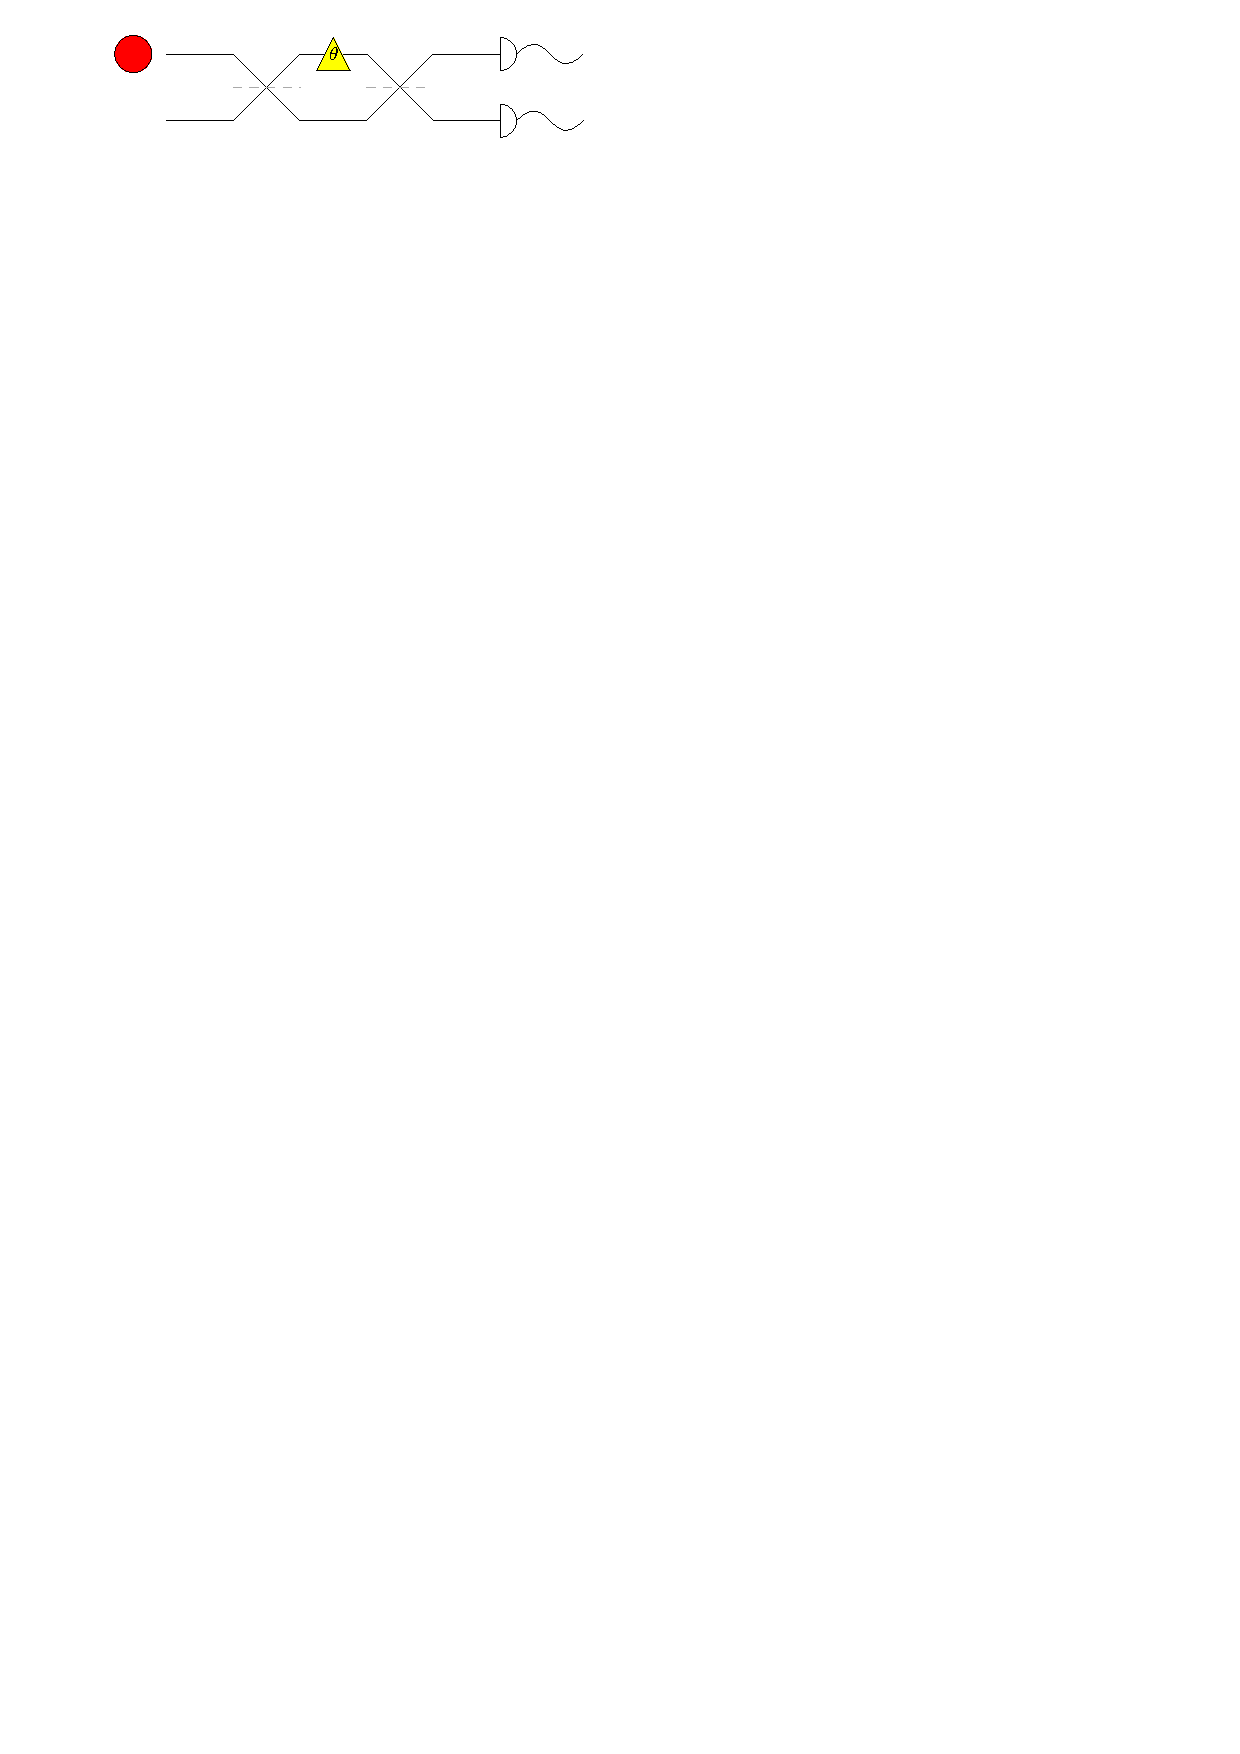
\includegraphics[width=0.45\linewidth]{preliminary_bs/mzi}}
\hfill
\subfloat[\label{fig:mzi-plot}]{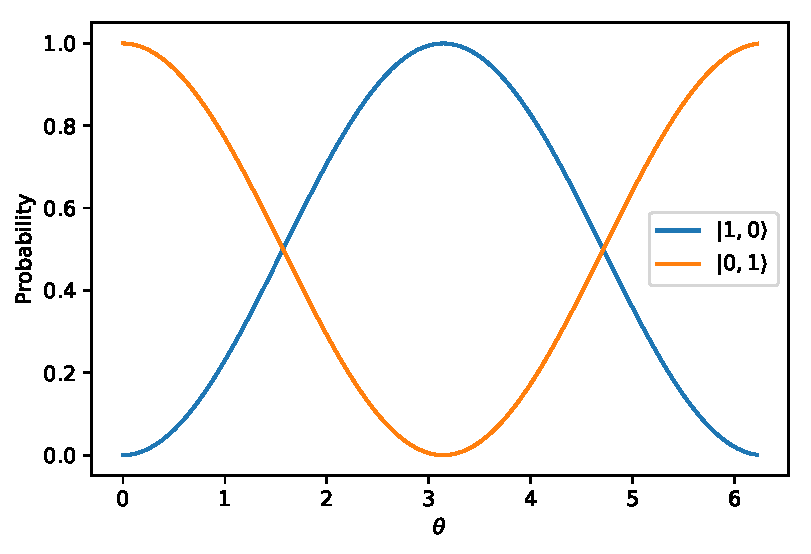
\includegraphics[width=0.45\linewidth]{preliminary_bs/mzi_plot}}
\caption[Experimental setup of the Mach-Zehnder Interferometer and probability of outcomes over phase $\theta$]{\label{fig:mzi}The Mach-Zehnder Interferometer, a demonstration of single-photon interference. \ref{fig:mzi-diagram}: An experimental diagram, consisting of a single photon (red circle) in one of two spatial modes (solid black lines), a phase shifter (yellow triangle containing $\theta$) surrounded by two 50-50 beam splitters (grey dashed lines) and single photon detectors (white semi-circles). \ref{fig:mzi-plot}: The Probability of measuring $\ket{0,1}$ (orange) and $\ket{1,0}$ (blue) from a Mach-Zehnder Interferometer over $\theta$.}
\end{figure}

A Mach-Zehnder Interferometer (MZI) is a demonstration of how a single photon can interfere with itself \cite{zehnder1891,mach1892}. This experiment uses a single photon in one of two modes, and consists of a 50-50 beam splitter across both modes, followed by a phase shifter on a single mode, and finally a second 50-50 beam splitter. A diagram of this experiment can be seen in Figure \ref{fig:mzi-plot}.

In second quantisation, we can describe the MZI as follows, labelling our spatial modes 1 and 2. We start with a single photon in mode 1 $\ket{1,0} = a_1^\dagger\ket{0,0}$. After our first beam splitter we have the state $(a_1^\dagger + ia_2^\dagger)\ket{0,0}/\sqrt{2} = (\ket{1,0}+i\ket{0,1})/\sqrt{2}.$

We next apply a phase shifter to spatial mode 1, giving $(e^{i\theta}a_1^\dagger + ia_2^\dagger)\ket{0,0}/\sqrt{2}$. Finally, we apply our second beam splitter and find that

\begin{align}
\frac{1}{\sqrt{2}}(e^{i\theta}a_1^\dagger + ia_2^\dagger)\ket{0,0} &\rightarrow \frac{1}{2}(e^{i\theta}(a_1^\dagger+ia_2^\dagger) + i(ia_1^\dagger + a_2^\dagger))\ket{0,0}\\
&= \frac{1}{2}((e^{i\theta}-1)a_1^\dagger+i(e^{i\theta}+1)a_2^\dagger)\ket{0,0}.
\end{align}

Adjusting our phase $\theta$ determines what output we measure: For $\theta=0$, the photon will be in mode 2; for $\theta=\pi/2$, the photon will be in mode 1, and for other values of $\theta$ the photon will be measured randomly in one of the two modes. How the probabilities change over $\theta$ is given in Figure \ref{fig:mzi-plot}.

In first quantisation, we see the same outcome. Our input is $\ket{1}$, and  applying the first beam splitter leads to the state $(\ket{1}+i\ket{2})/\sqrt{2}$. The phase shifter on mode 1 results in the state $(e^{i\theta}\ket{1}+i\ket{2})/\sqrt{2}$, and the second beam splitter leaves us with the state

\begin{align}
\ket{\psi} &= \frac{1}{2}\left(e^{i\theta}\left(\ket{1} + i\ket{2}\right) + i\left(i\ket{1} + \ket{2}\right)\right)\\
&= \frac{1}{2}\left(\left(e^{i\theta}-1\right)\ket{1} + i\left(e^{i\theta}+1\right)\ket{2}\right).
\end{align}

Again, we see that adjusting $\theta$ will determine which spatial mode we detect a photon in.

\subsubsection{Two-photons-two-modes: The Hong-Ou-Mandel Dip}

\begin{figure}
\begin{center}
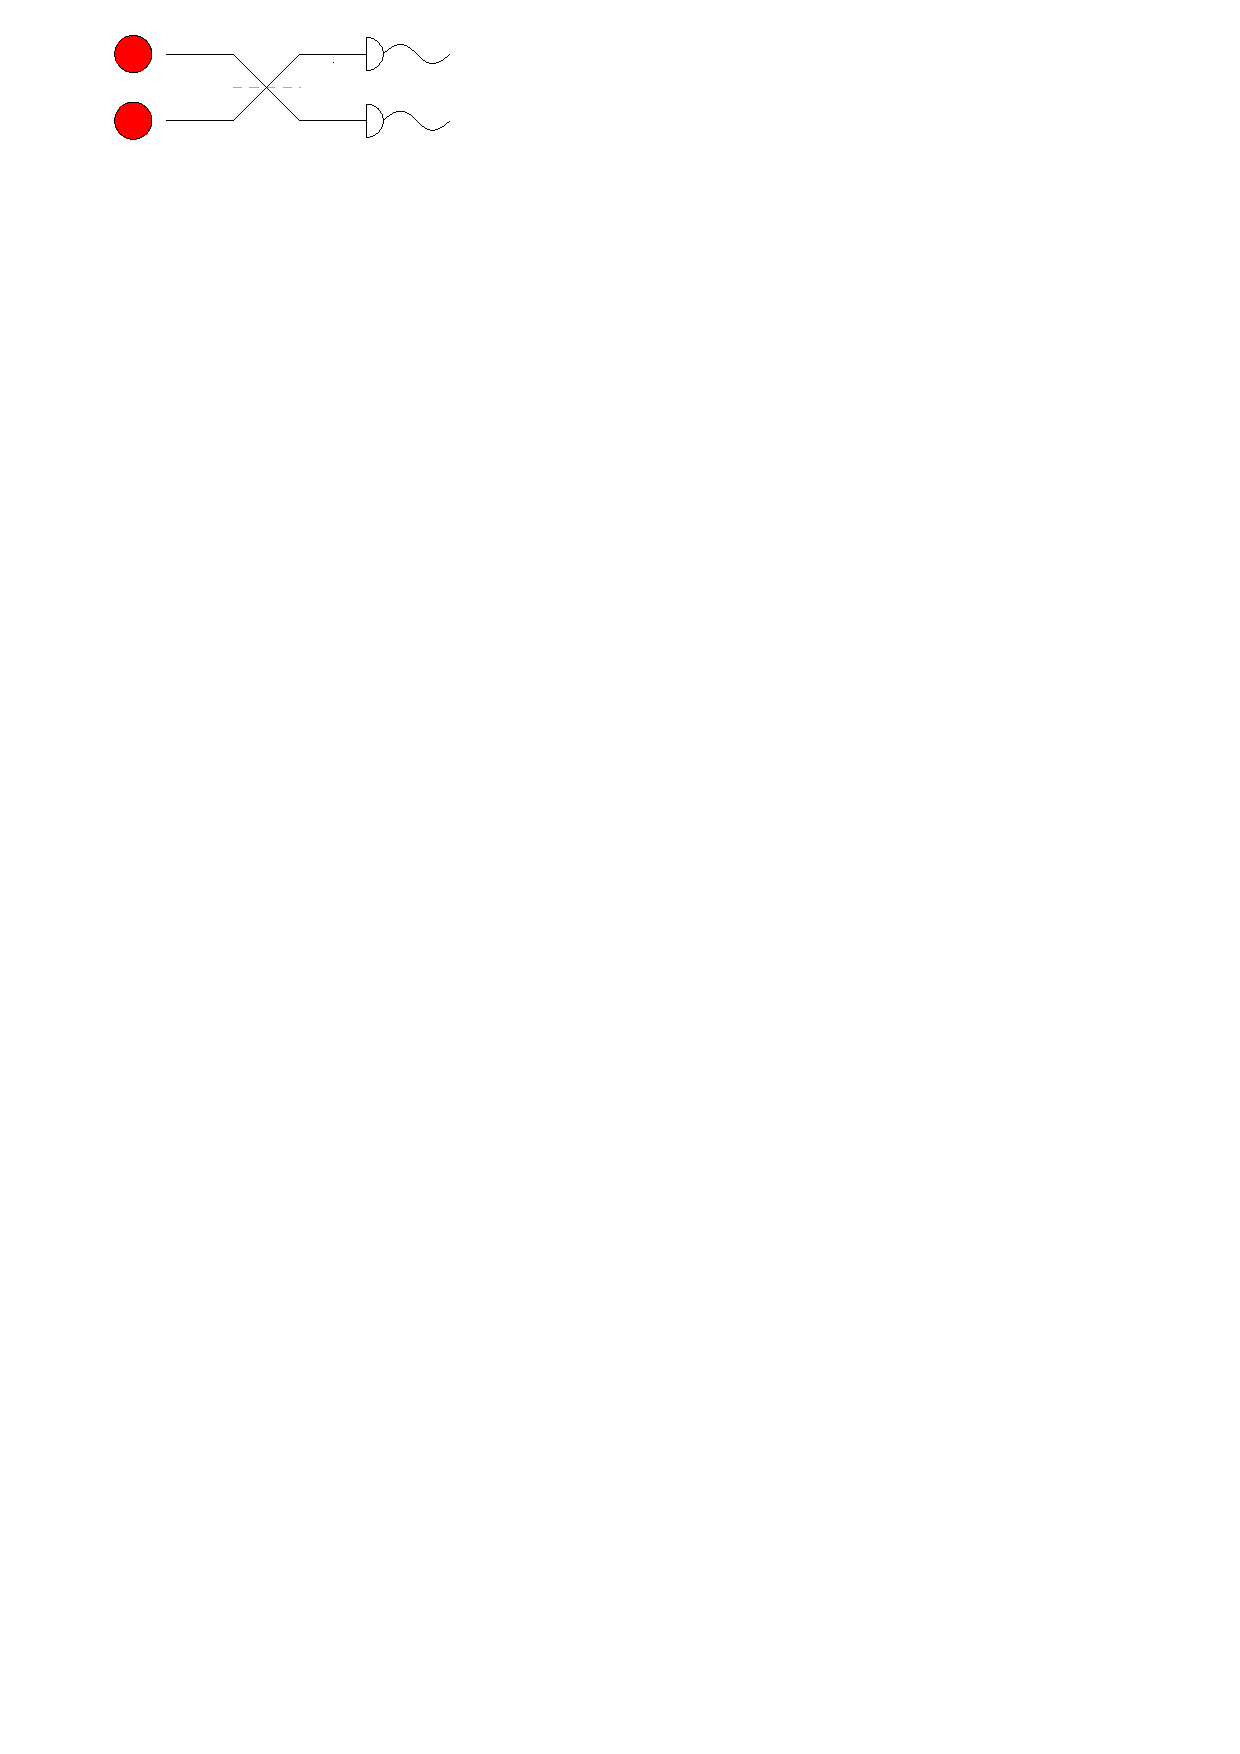
\includegraphics[width=0.45\linewidth]{preliminary_bs/hom}
\end{center}
\caption[Experimental setup of the Hong-Ou-Mandel Dip]{\label{fig:hom}An experimental diagram for the Hong-Ou-Mandel Dip, consisting of two indistinguishable photons (red circles) in two spatial modes (solid black lines) interacting with a single 50-50 beam splitter (grey dashed line) before being measured by single photon detectors (white semi-circles).}
\end{figure}

The Hong-Ou-Mandel (HOM) Dip is the earliest demonstration of multi-photon interference \cite{hong1987}. It features two spatial modes, each starting with a single photon, and consists of simply a 50-50 beam splitter across both modes.

In second quantisation, we start with the Fock state $\ket{1,1} = a_1^\dagger a_2^\dagger\ket{0,0}$. Applying the beam splitter gives us

\begin{align}
a_1^\dagger a_2^\dagger\ket{0,0} &\rightarrow \frac{1}{2}(a_1^\dagger+ia_2^\dagger)(ia_1^\dagger+a_2^\dagger)\ket{0,0}\\
&= \frac{1}{2}\left(i(a_1^\dagger)^2+a_1^\dagger a_2^\dagger-a_2^\dagger a_1^\dagger+i(a_2^\dagger)^2\right)\ket{0,0}\\
&= \frac{1}{2}\left(i(a_1^\dagger)^2+a_1^\dagger a_2^\dagger-a_1^\dagger a_2^\dagger+i(a_2^\dagger)^2\right)\ket{0,0}\\
&= \frac{i\left((a_1^\dagger)^2+(a_2^\dagger)^2\right)}{2}\ket{0,0}\\
&= \frac{i(\ket{2,0} + \ket{0,2})}{\sqrt{2}}.
\end{align}

After measurement, we will find that both photons will always be detected in the same (random) spatial mode. This example has a strong connection to distinguishability, and we will return to it in Section \ref{ssec:imperfections-distinguishability}.

In first quantisation, we start with the state $(\ket{12} + \ket{21})/\sqrt{2}$. The beam splitter acts on each particle individually, giving

\begin{align}
\ket{\psi} &= \frac{1}{2\sqrt{2}}\left(\left(\ket{1} + i\ket{2}\right)\left(i\ket{1} + \ket{2}\right) + \left(i\ket{1} + \ket{2}\right)\left(\ket{1} + i\ket{2}\right)\right)\\
&= \frac{1}{2\sqrt{2}}\left(2i\ket{11} + (1+i^2)\ket{12} + (i^2+1)\ket{21} + 2i\ket{22}\right)\\
&= \frac{i(\ket{11}+\ket{22})}{\sqrt{2}}.
\end{align}

Again, we find that only bunching is observed at the output.

\subsection{Bosonic sampling}
\label{ssec:bosonic-sampling}

We now define the ideal probability distribution of indistinguishable single bosons interacting on a linear interferometer.
We'll refer to this as bosonic sampling, as it's a bit more general than Aaronson and Arkhipov's Boson Sampling problem as we describe below.
The input is $U \in \mathrm{U}(m)$, an $m\times m$ unitary matrix which describes an $m$-mode linear interferometer, and $S = (S_1,S_2,\dots,S_m)$ with $\sum_{i=1}^m S_i =n$, an ordered list of integers that corresponds to an $n$-boson, $m$-mode occupation describing the input state with $S_i$ bosons in mode $i$. 
Given an output occupation $S'$, define the $n \times n$ (not necessarily unitary) matrix $U_{S',S}$ as that formed by first taking $S_i'$ copies of row $i$ of $U$ in order to create an $m\times n$ matrix, from which we then take $S_j$ copies of column $j$. 
We can then define $\mathcal{D}_{U,S}$, the probability distribution for measuring an $n$-boson $m$-mode occupation $S'$ for interferometer $U$ and input state $S$, as
\begin{equation}\label{eqn:bs-distribution}
\textrm{Pr}_{\mathcal{D}_{U,S}}[S'] = \frac{|\per(U_{S',S})|^2}{\prod_{i=1}^m S_i'! S_i!} ,
\end{equation}
where $\per$ is the matrix permanent, defined as

\begin{equation}
\per(M) = \sum_{\sigma\in\symm_n}\prod_{i=0}^nM_{i,\sigma(i)}.
\label{eqn:permanent}
\end{equation}

This relationship between linear optics and matrix permanents was originally found by Scheel and Buhmann \cite{scheel2008}, and later proven by Aaronson and Arkhipov using a different approach \cite{aaronson2010report, aaronson2011}.

In a photonics experiment, this setting is described in terms of creation operators $a^\dag_i$ for a photon in mode $i$. 
The initial state is then
\begin{equation}
|S\rangle = \prod_{i=0}^m \frac{(a_i^\dagger)^{S_i}}{\prod_{j=2}^{S_i}\sqrt{j}}|0^m\rangle.
\end{equation}
The evolution of the photonic state induced by a linear optical interferometer implementing $U$ can then be expressed as $a_i^\dagger \mapsto \sum_{j = 0}^m U_{i,j}a_j^\dagger$.
Thus single boson states evolve under linear interferometry just as an $m$ dimensional qudit does under a unitary gate $U$ (sometimes called unary encoding).
This suggests how quantum circuits simulating photonics might be constructed, as we'll see.

The problem known as Boson Sampling is that of sampling from this probability distribution under certain conditions \cite{aaronson2010report, aaronson2011}. First, the input occupation is specified as $|1^n 0^{m - n}\rangle = \prod_{i = 1}^n a_{i}^\dagger|0\rangle$. Second, the interferometer $U$ is sampled Haar randomly from U$(m)$ with $m=O(n^2)$. And finally, the sampled output is anti-bunched, meaning that there is at most one photon in each spatial mode. Such a photon occupation is also referred to as coincident. Although it looks like this last condition relies on postselection and could therefore be costly in practice, it can be satisfied with high probability if $m=O(n^2)$, due to the Bosonic Birthday Paradox \cite{arkhipov2011}.

It is easy to see that both of the two examples discussed in Section \ref{ssec:example-interferometers} can be described in this picture as well. For the Mach-Zehnder Interferometer, we find that the unitary matrix describing our interferometer is

\begin{align}
U &= \frac{1}{2}\begin{pmatrix}1&i\\i&1\end{pmatrix}\begin{pmatrix}e^{i\theta}&0\\0&1\end{pmatrix}\begin{pmatrix}1&i\\i&1\end{pmatrix}\\
&= \frac{1}{2}\begin{pmatrix}e^{i\theta}&i\\ie^{i\theta}&1\end{pmatrix}\begin{pmatrix}1&i\\i&1\end{pmatrix}\\
&= \frac{1}{2}\begin{pmatrix}e^{i\theta}-1&i(e^{i\theta}+1)\\i(e^{i\theta}+1)&1-e^{i\theta}\end{pmatrix}.
\end{align}

Assuming our photon is initially in mode 1, the relevant matrices describing our outcomes are the $1\times 1$ matrices $M_{1,1} = e^{i\theta}-1$ and $M_{1,2} = i(e^{i\theta}+1)$. For $1\times 1$ matrices the permanent is just the single element, and so we find the probabilities are $|e^{i\theta}-1|^2$ and $|e^{i\theta}+1|^2$, giving us the expected outcome of controlling the photon output based on $\theta$.

For the Hong-Ou-Mandel Dip, we note that the relevant unitary matrix is the matrix we have for a beam splitter. We then note that the probability of seeing outcome occupation $\ket{1,1}$ is

\begin{align}
\left|\per\begin{pmatrix}\frac{1}{\sqrt{2}}&\frac{i}{\sqrt{2}}\\\frac{i}{\sqrt{2}}&\frac{1}{\sqrt{2}}\end{pmatrix}\right|^2 &= \frac{|1+i^2|^2}{4}\\
&= 0.
\end{align}

Similarly we find that the outcomes for $\ket{2,0}$ and $\ket{0,2}$ are

\begin{align}
\frac{\left|\per\begin{pmatrix}\frac{1}{\sqrt{2}}&\frac{i}{\sqrt{2}}\\\frac{1}{\sqrt{2}}&\frac{i}{\sqrt{2}}\end{pmatrix}\right|^2}{2!} &= \frac{|2i|^2}{8}\\
&= \frac{1}{2},
\end{align}

\noindent and

\begin{align}
\frac{\left|\per\begin{pmatrix}\frac{i}{\sqrt{2}}&\frac{1}{\sqrt{2}}\\\frac{i}{\sqrt{2}}&\frac{1}{\sqrt{2}}\end{pmatrix}\right|^2}{2!} &= \frac{|2i|^2}{8}\\
&= \frac{1}{2},
\end{align}

\noindent respectfully. This matches the expected outcome statistics of the coincident output never occurring and the two other possible outcomes happening purely at random.

\subsection{Universal linear optical interferometers}
\label{ssec:universal-lo}

\begin{figure}
\subfloat[\label{fig:reck}]{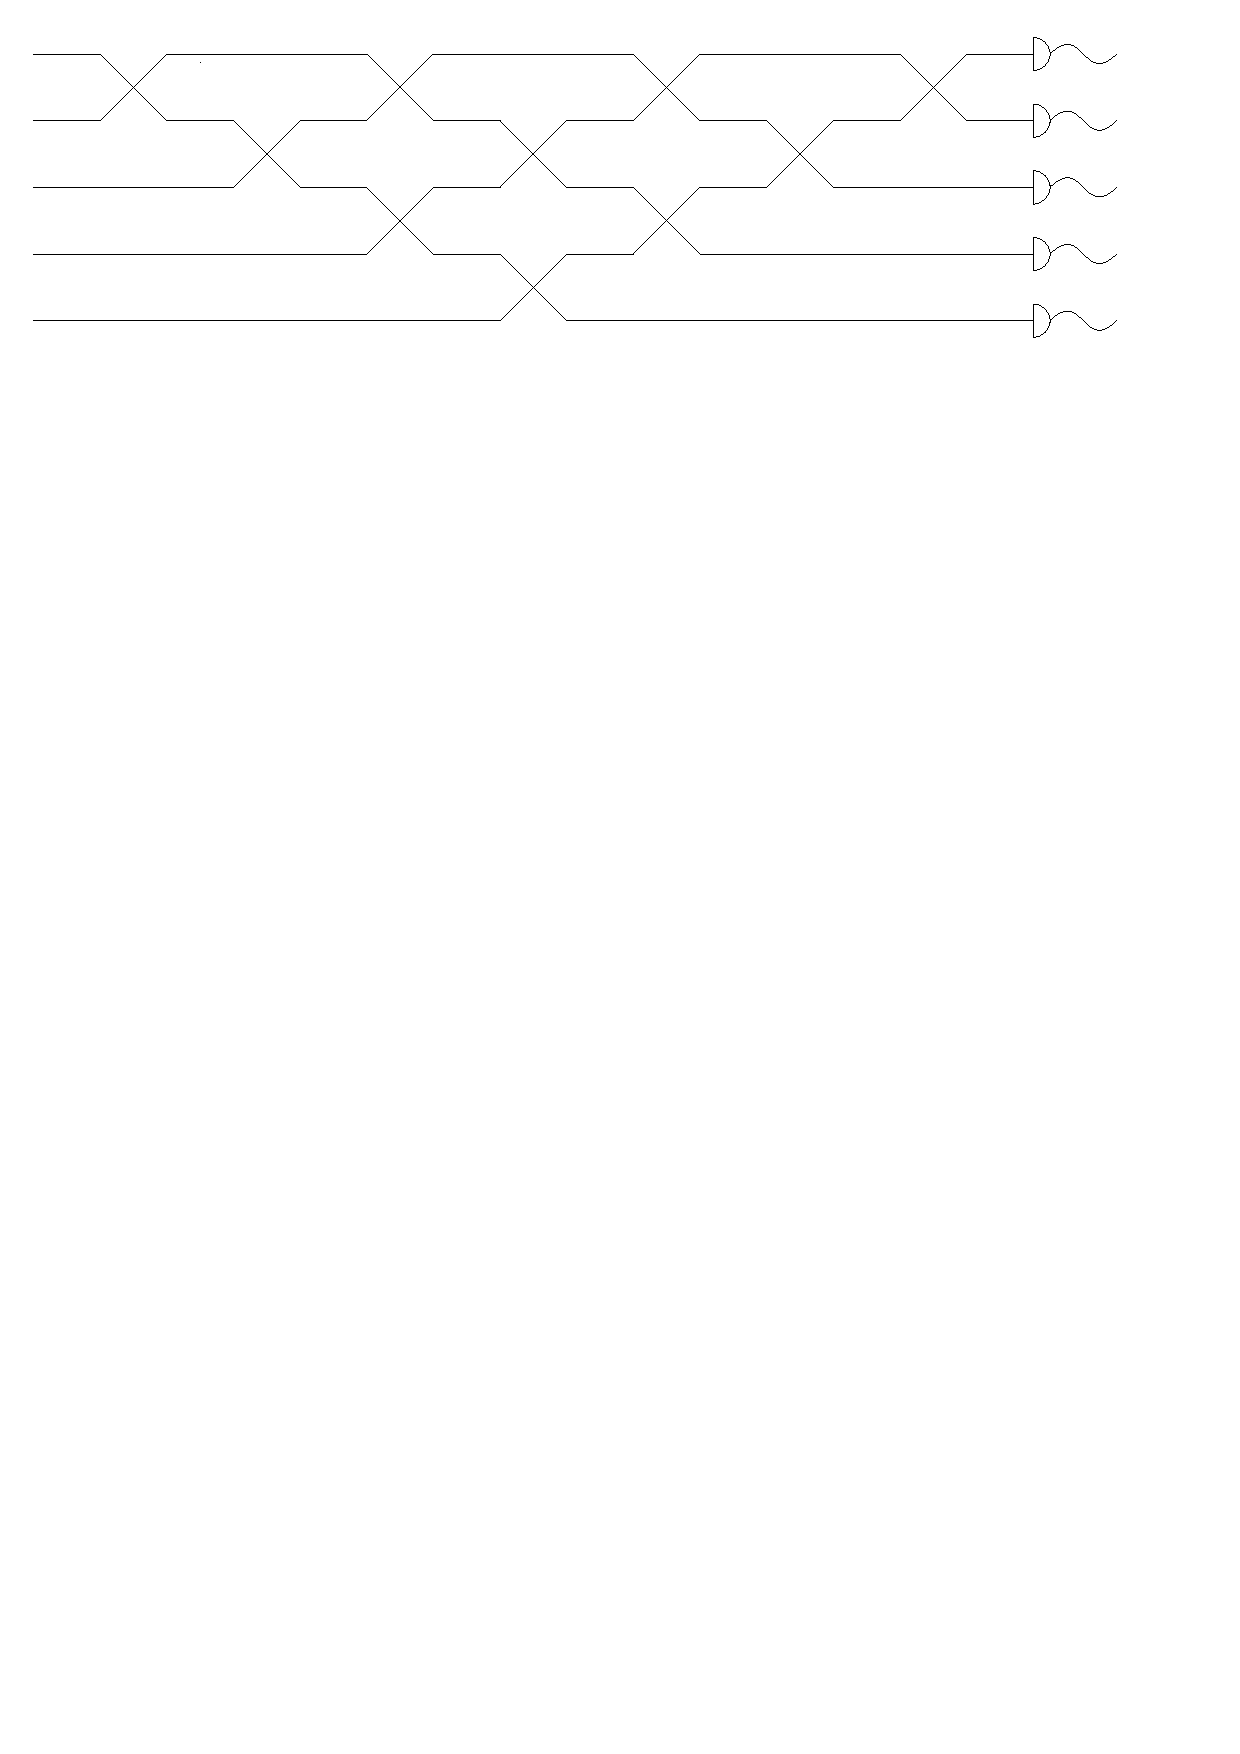
\includegraphics[width=0.45\linewidth]{preliminary_bs/reck}}
\hfill
\subfloat[\label{fig:clements}]{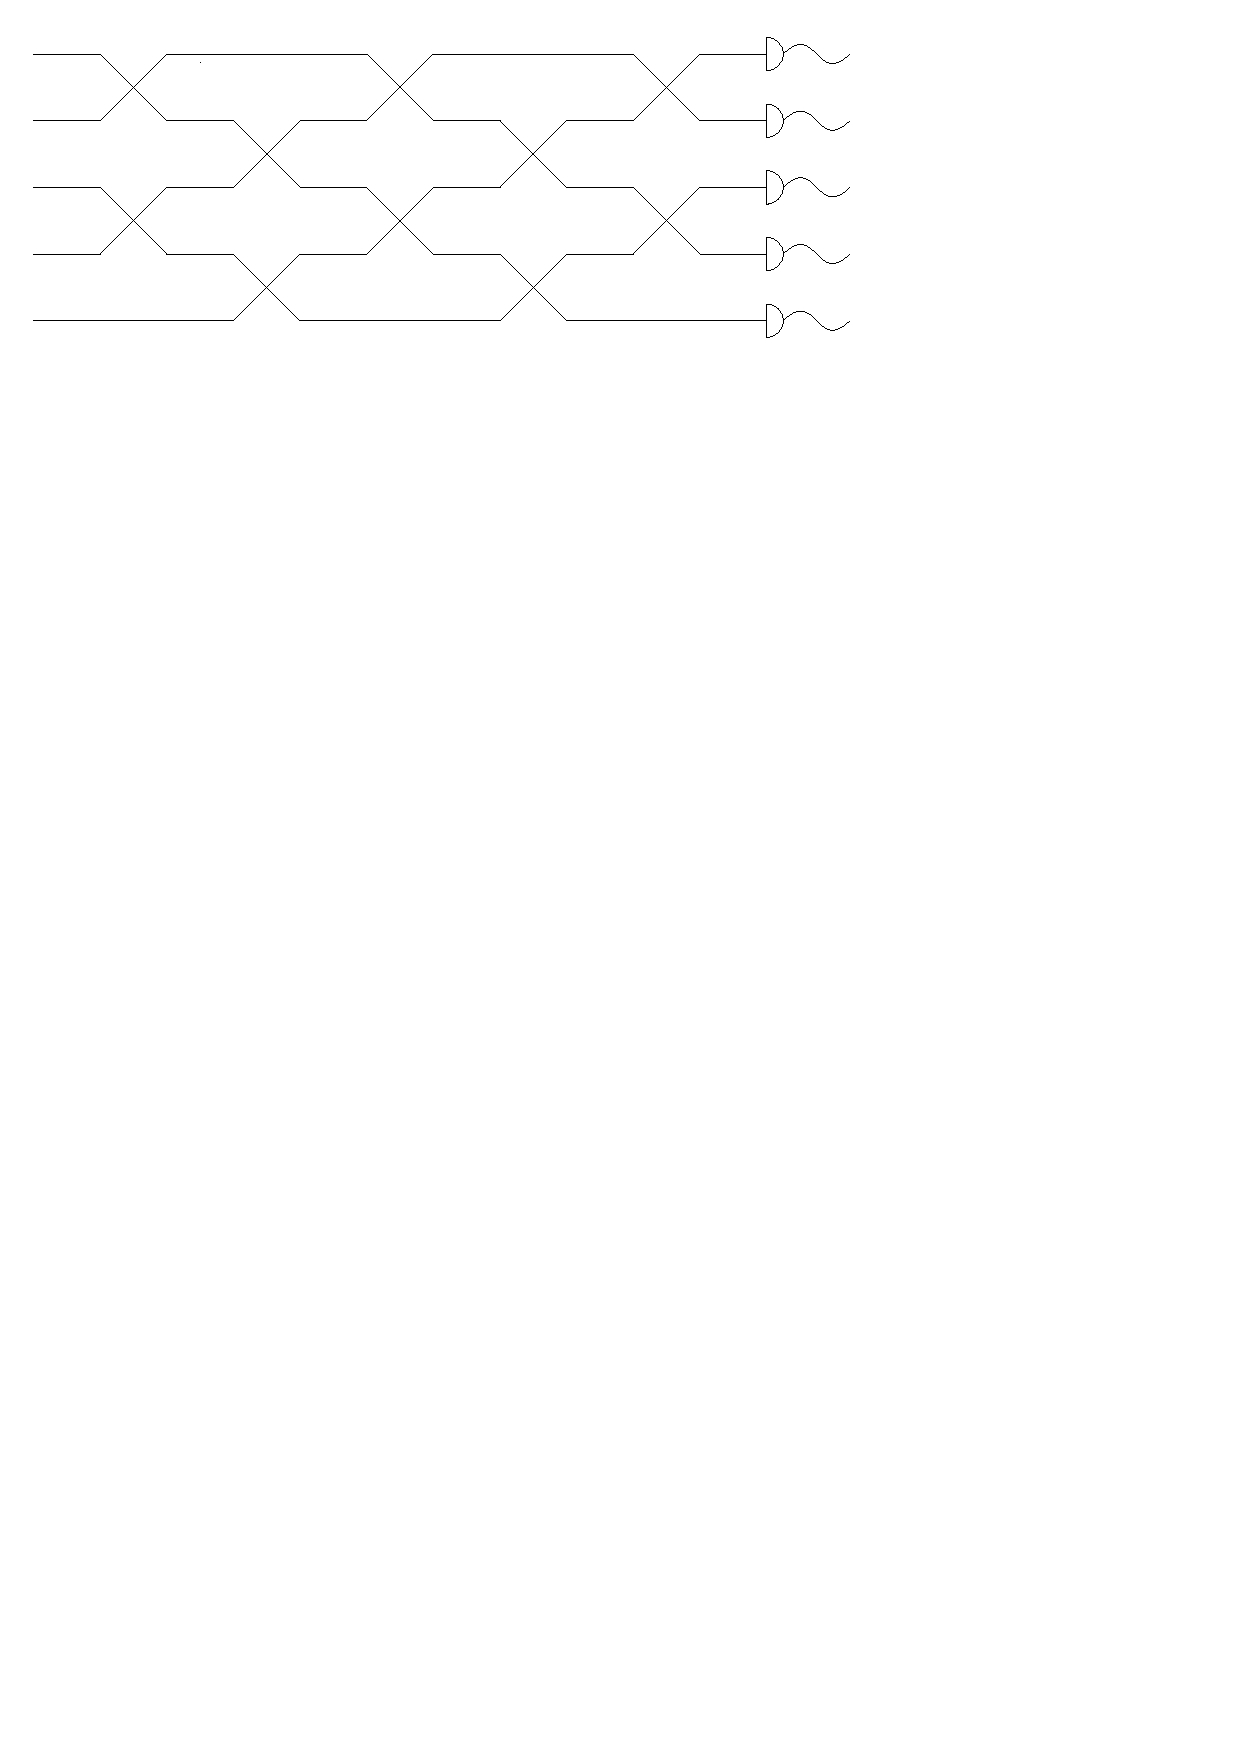
\includegraphics[width=0.45\linewidth]{preliminary_bs/clements}}
\caption[Two examples of universal linear-optical interferometers]{\label{fig:universal-lo}Two examples of universal linear-optical interferometers by (\ref{fig:reck}) Reck et al.~\cite{reck1994} and (\ref{fig:clements}) Clements et al.~\cite{clements2016}. Each point where two spatial modes overlap is a Mach-Zehnder interferometer, as described in Section \ref{ssec:example-interferometers}.}
\end{figure}

One of the requirements of Boson Sampling is that the unitary $U$ should be Haar-random. Choosing a unitary purely at random might seem like a challenge at first, but there are examples of linear optical interferometers which are fully reprogrammable. We will give two examples, from which any unitary can be implemented by reprogramming the phase shifters.

The first of these schemes was realised mathematically by Hurwitz, and later rediscovered by Reck et al.~\cite{hurwitz1897, reck1994}. This scheme uses a sequence of Mach-Zehnder Interferometers arranged in a pyramid-like structure, shown in Figure \ref{fig:reck}. The universality of this scheme is proven recursively, by decomposing an $m\times m$ unitary matrix into an $(m-1)\times(m-1)$ unitary matrix accompanied by $m$ two-mode transformations in the $m$-th mode. These additional transformations can be implemented as MZIs. However, a potential weakness with this interferometer is that it is of very high depth; a photon starting and finishing in mode 1 might interact with up to $2m-3$ beam splitters. This could result in experiments being impractically large, and also result in issues such as photon loss, something we will discuss further in Section \ref{ssec:imperfections-loss}.

These issues were addressed in a later interferometer designed by Clements et al.~\cite{clements2016}. This design is similarly constructed out of MZIs, arranged in a chequerboard-like design alternating between pairs of modes, shown in Figure \ref{fig:clements}. The universality of this design is proven by decomposing the diagonals along either side of $U$ into two-mode transformations. This design has depth $m$, lower than that of the Hurwitz scheme above. It is also easy to see that a lower depth scheme is impossible, as a photon in mode 1 would then not be able to reach mode $m$.

For the specific case of Boson Sampling, Aaronson and Arkhipov showed that the circuit depth required can be improved even further \cite{aaronson2011, aaronson2010report}. This is because the only input we provide to $U$ is the Fock state $\ket{1^n0^{m-n}}$. It is therefore sufficient for us to consider some interferometer $\tilde{U}$ which, when applied to $\ket{1^n0^{m-n}}$, produces the same state as $U$. Aaronson and Arkhipov describe such an interferometer on $m+n$ modes which uses $O(mn)$ components and has depth $O(n\log m)$, which is an improvement over the Hurwitz and Clements schemes if $n=O(m^2)$. Note that a crucial assumption underlying this proof is that swapping mode $i$ with mode $m+i$ is a constant-depth operation. For 2D photonic circuits, where spatial mode $i$ is only coupled with modes $i-1$ and $i+1$, such an operation would require $O(m)$ depth and therefore lose all advantage. This setup also requires that we only apply $U$ to the input state $\ket{1^n0^{m-n}}$, which does not hold for the variants of Boson Sampling we discuss in Section \ref{ssec:bs-variants}.

\subsection{The computational complexity of Boson Sampling}
\label{ssec:cc-bs}

\begin{problem}[Boson Sampling] Let $U$ be an $m$-mode linear optical interferometer. Sample from the distribution corresponding to measuring $U$ acting on $|1^n0^{m-n}\rangle$ in the (anti-bunched) Fock basis, where $m=O(n^2)$.
\end{problem}

It was proven by Aaronson and Arkhipov that if there was a polynomial time classical algorithm for sampling from this distribution, then $\p^{\sharpp} = \bpp^{\np}$ and the Polynomial Hierarchy would collapse to the third level \cite{aaronson2010report, aaronson2011}. This is done using the fact that the permanent of a matrix is $\sharpp$-hard, even to approximate \cite{valiant1979, aaronson2011sharpp}. 
Aaronson and Arkhipov also showed the same result for sampling from any approximate distribution up to $\epsilon$ away in total variation distance from Boson Sampling, assuming the conjectures from before.

In comparison to the other quantum advantage problems, the anticoncentration conjecture has not been proven for Boson Sampling. It is also not known if it is $\sharpp$-hard to approximate the permanent of a random complex matrix, however it has been proven that exactly computing the permanent of a Gaussian matrix is $\sharpp$-hard \cite{aaronson2010report, aaronson2011}.

Regarding the question of verifying Boson Sampling, there have been some interesting results. Gogolin et al.~\cite{gogolin2013} argued that if a verifier does not know the underlying distribution, and is therefore only using the samples obtained to verify the distribution, then Boson Sampling requires an exponentially large number of samples to differentiate from the uniform distribution. This was refuted by Aaronson and Arkhipov \cite{aaronson2014}, who argued that this definition of a verifier is poor, akin to arguing that factoring an integer into its prime factors $N=pq$ should not be verified by multiplying $p$ and $q$ together, or that a Hamiltonian cycle in a graph shouldn't be verified by ensuring every vertex is visited exactly once. Aaronson and Arkhipov then develop further on this result, first showing that Boson Sampling is far from the uniform distribution in total variation distance, and then providing an explicit estimator which can discriminate Boson Sampling from the uniform distribution. But there are other classical distributions, notably Boson Sampling with fully distinguishable photons, which the algorithm fails to distinguish. This was resolved in work by Spagnolo et al.~\cite{spagnolo2014}, who experimentally implemented the uniform discriminator and developed another algorithm which could differentiate ideal Boson Sampling from Boson Sampling with fully distinguishable photons. Agresti et al.~\cite{agresti2019} later used the $K$-means clustering algorithm from machine learning, with a three-photon Boson Sampling experiment providing the target data, to discriminate between indistinguishable and distinguishable Boson Sampling as well. Agresti et al.\ then used classical Boson Sampling simulators (see Section \ref{sec:classical-simulations}) to test how effective their discriminator was using the same original test data to distinguish experiments with up to 25 photons across up to 625 modes, and found that in most cases $10^4$ samples were sufficient to distinguish the two distributions.

As we shall see in Section \ref{sec:experimental-achievements}, distinguishing from the two distributions above is a common technique for verifying Boson Sampling experiments today \cite{carolan2015, zhong2018, paesani2018, wang2019}. However, it is still unclear what properties can be used to fully distinguish Boson Sampling from other distributions which can be classically simulated. One proposal by Carolan et al.~\cite{carolan2014} was to use photon bunching to characterise effects, but this was quickly refuted by Tichy et al.~\cite{tichy2014}, who gave a Monte Carlo algorithm which could output a distribution with the same properties. Walschaers et al.~\cite{walschaers2016, walschaers2016thesis} later provided more refined statistical features from random matrix theory which can discriminate against all models discussed so far for $m<n^{5.1}$. Giordani et al.~\cite{giordani2018} demonstrate this experimentally, and use machine learning to identify what characteristics give way to these features. However, even with these approaches as $m$ and $n$ increase the distributions start to become more alike.

\subsection{Boson Sampling variants}
\label{ssec:bs-variants}

Since originally being proposed, a number of Boson Sampling variants have arisen to varying degrees of success, which aim to fix experimental challenges in vanilla Boson Sampling. We give two particular examples below which have been experimentally realised.

\begin{problem}[Scattershot Boson Sampling] Let $U$ be an $m$-mode linear optical interferometer. Sample from the distribution corresponding to measuring $U$ acting on $|\bar{S}\rangle$ in the (anti-bunched) Fock basis, where $m=O(n^2)$ and conditioned on sampling $\bar{S}$ uniformly at random from the $\binom{m}{n}$ ways of choosing $n$ out of $m$ input modes.
\end{problem}

One of the largest issues with Boson Sampling is generating the input state $\ket{1^n0^{m-n}}$. This is because we do not currently have deterministic single photon sources \cite{eisaman2011}. If a single photon source outputs a photon with probability $p$, $n$ independent sources will all generate single photons with probability $p^n$, so we will have to wait an exponentially long time just to generate enough photons.

The idea of Scattershot Boson Sampling is to increase the number of probabilistic photon sources and condition the distribution on which sources output a photon \cite{aaronson2013, lund2014}. This can be implemented experimentally by using heralded sources, which use nonlinear optical effects such as Spontaneous Parametric Down Conversion to generate a pair of photons of different wavelengths \cite{loudon2006}. By measuring one of these photons, we know that a pair of photons were generated in this spatial mode and therefore we can input the other photon to our interferometer. Now if there are $n$ heralded sources each firing with probability $p$, then we expect on average $np$ photons to be input to our interferometer.

It is worth noting that with heralded photon sources there is also a probability that more than one pair of photons is generated by a single source. Although it is not fully clear how the computational hardness is affected when multiple photons are generated in the same mode, it is known that photons generated in the same spatial mode do not interfere with each other. We can avoid this scenario by limiting the probability of a successful herald. Christ and Silberhorn estimate that a heralding probability of $25\%$ is optimal for achieving the best success rate while also minimising multi-photon emissions, and recommend active switching to improve heralding rates even further \cite{christ2012}.

\begin{problem}[Gaussian Boson Sampling] Let $U$ be an $m$-mode linear optical interferometer. Sample from the distribution corresponding to measuring $U$ acting on $|\zeta^n0^{m-n}\rangle$ in the (anti-bunched) Fock basis, where $m=O(n^2)$ and $|\zeta\rangle$ is a single mode squeezed vacuum state.
\end{problem}

Gaussian Boson Sampling is another proposed way of working around the need for single photon sources \cite{hamilton2017}. The idea is to start with $k\approx n$ single mode squeezed states, each generated from the $\ket{0}$ Fock state. These squeezed states are then input into an interferometer and measured in the Fock basis.

Hamilton et al.~\cite{hamilton2017} used arguments akin to Aaronson and Arkhipov to argue that Gaussian Boson Sampling is computationally hard. The main difference between the two is that the probability of a particular output from Gaussian Boson Sampling is proportional to another $\sharpp$-Hard function called the Hafnian of a $2n\times 2n$ matrix, rather than the permanent of an $n\times n$ matrix. From this starting point the rest of the argument follows through. Another intuitive way of seeing this is in Aaronson, courtesy of Garc\'{i}a-Patr\'{o}n \cite{aaronson2013}, by noting that Scattershot Boson Sampling can be reduced to Gaussian Boson Sampling. To do this, we simply embed the photon pair sources into the Gaussian Boson Sampling experiment by generating two-mode entangled squeezed states and using them as input.

Another unexpected benefit of Gaussian Boson Sampling is that there are some applications demonstrated. Huh, et al.~\cite{huh2015} showed that Gaussian Boson Sampling could be used to simulate the vibronic spectra of molecules. It has also recently been that graphs can be encoded into Gaussian Boson Sampling experiments to solve various problems including Graph Isomorphism and finding dense subgraphs \cite{bradler2018, schuld2019, arrazola2018}, though it is unclear how these techniques fare against the best classical algorithms \cite{aaronson2019mottebailey}.

It is worth noting that measuring in the Fock basis is crucial for computational hardness in Gaussian Boson Sampling. In particular, if the measurement is instead a Homodyne measurement for measuring Gaussian states, the resulting distribution is classically simulable in polynomial time \cite{bartlett2003}.

\section{Experimental Achievements}
\label{sec:experimental-achievements}

Since originally being proposed in 2010, Boson Sampling has taken the interest of a number of quantum optics research groups, each eager to demonstrate a quantum advantage through this process. We provide some of the results of said groups below.

The earliest experimental demonstrations were shown in 2013, by four different groups independently \cite{broome2013, spring2013, tillmann2013, crespi2013}. These results were published simultaneously, with two publications in \emph{Nature Photonics} and two in \emph{Science}. All four results used reprogrammable designs on integrated photonic circuits to implement the unitary transformation. Crespi et al.~\cite{crespi2013} and Tillmann et al.~\cite{tillmann2013} both demonstrated Boson Sampling with up to three photons across five modes. Broome et al.~\cite{broome2013} demonstrated three photons across six spatial modes, while Spring et al.~\cite{spring2013} demonstrated four photons across six modes. Crespi et al., Broome et al., and Spring et al., verified their experimental results by computing the distance between their experimental distribution and the theoretical distribution \cite{spring2013, tillmann2013, crespi2013}, while Tillman et al.\ verified their experiment by estimating the fidelity \cite{tillmann2013}.

Later in 2015, an experiment by Carolan et al.~\cite{carolan2015} demonstrated experimental Boson Sampling with six photons across six modes. This was implemented on a fully reprogrammable integrated silica circuit. One caveat is that the authors used the input Fock state $\ket{3,3,0,0,0,0}$, rather than the traditional form of having single photons in each mode. The authors justify this in order to use the verification approach of \cite{carolan2014}, though as discussed in Section \ref{ssec:cc-bs} this verification approach has limitations of its own. This device was later also used by Sparrow, Mart\'{i}n-L\'{o}pez et al.~\cite{sparrow2018} with two-mode squeezed inputs and adaptive feedback to simulate the vibronic structure of a variety of 4-atom molecules, hinting at a potential application for bosonic sampling.

The first Boson Sampling demonstration with five single photons was performed in 2017 by Wang et al.~\cite{wang2017}. Wang et al.\ used a triangular array of beam splitters bonded together to create a structure smaller than regular bulk optics but larger than integrated silicon or silica chips, featuring 9 input and output modes. Wang et al.\ state that many interferometers can be generated from this chip by adjusting the polarisation of photons, but acknowledge that the structure itself is not universal. Boson Sampling is verified in this experiment by checking against the uniform and fully distinguishable distributions.

Following this came a few results on up to five photons for Boson Sampling variants. Zhong et al.~\cite{zhong2018} demonstrated Scattershot Boson Sampling with up to five photons across twelve modes, using an interferometer constructed by six trapezoidal quartz blocks covered in film and fused together. Then, Paesani et al.~\cite{paesani2018} demonstrated four photon Scattershot, Gaussian and vanilla Boson Sampling on a single integrated silicon chip, by simply adjusting which state they input to the chip. Finally, Zhong et al.~\cite{zhong2019} demonstrated Gaussian Boson Sampling with up to five photons, using the same interferometer as in \cite{zhong2018}. All of the standard and Scattershot Boson Sampling experiments were validated by comparison to distinguishable and uniform sampling. In the case of Gaussian Boson Sampling, comparisons were also made to thermal states, non-squeezed coherent states and two-mode squeezed states, as well as demonstrating applications related to molecular simulations and graph theory \cite{paesani2018, zhong2019}.

The most recent experimental demonstration of Boson Sampling was performed in 2019 by Wang et al.~\cite{wang2019}. This experiment used a 3D integrated photonic circuit with 60 spatial modes. Wang et al.\ managed to demonstrate standard Boson Sampling with up to 10 photons, as well as Boson Sampling under loss with up to 20 input photons and 14 output photons, both of which were verified by comparison to uniform and distinguishable photon distributions. To date this is the largest demonstration of Boson Sampling publicly announced.

\section{Experimental Imperfections in Linear Optics}
\label{sec:lo-imperfections}

We shall now discuss two imperfections that are particularly common in Boson Sampling. The first is distinguishability, when one or more factors make bosons distinct from one another. The second, loss, is when photons which are generated at input are not detected at the output. We shall discuss some ways in which these issues occur, how they affect the probability distributions, and what is known about their computational complexity. In Section \ref{sec:classical-simulations}, we shall discuss some of the classical simulation algorithms that have been developed surrounding these issues.

\subsection{Distinguishability}
\label{ssec:imperfections-distinguishability}

One of the points made when discussing Boson Sampling is that the photons need to be indistinguishable. This means that if we permuted the photons in some way, it would be impossible for someone else to identify which permutation was applied.

A number of internal characteristics about the photons could make them distinguishable. The most visually intuitive one is wavelength: A red photon is definitely distinct from a green photon. But other aspects can also distinguish photons, such as their polarisation, or what time they were generated. The time generation point is particularly important following the discussion in Section \ref{ssec:bs-variants} about the challenges of single photon sources \cite{eisaman2011}: Not only do all of these single photon sources need to emit a photon, but all of them need to emit a single photon \textit{at the exact same time} \cite{aaronson2010report}. We can model distinguishability by introducing additional modes to describe the internal state. Throughout this thesis, we will use spatial or ``System'' modes to describe where a photon is, and internal or ``Label'' modes to describe its distinguishable characteristics.

Before we consider Boson Sampling with distinguishability, we will first return to the Hong-Ou-Mandel dip from Section \ref{ssec:example-interferometers} \cite{hong1987}. This time, we will consider one red photon generated in mode $1$, and one photon generated in mode 2 which is red with amplitude $v\in [0,1]$ and green with amplitude $d=\pm\sqrt{1-v^2}$. We can represent this in second quantisation by introducing additional indices to our creation and annihilation operators: $a_{i,R}^\dagger$ and $a_{i,G}^\dagger$ to indicate a red or green photon in mode $i$, respectively. Our input is now

\begin{equation}
a_{1,R}^\dagger\left(v a_{2,R}^\dagger + da_{2,G}^\dagger\right)\ket{0_R,0_G,0_R,0_G}.
\end{equation}

A beam splitter only affects System modes, and is invariant over Label modes. After applying the beam splitter our photons are in the state

\begin{align}
a_{1,R}^\dagger\left(v a_{2,R}^\dagger + da_{2,G}^\dagger\right)\ket{0_R,0_G,0_R,0_G} &\rightarrow \frac{1}{2}\left(a_{1,R}^\dagger + ia_{2,R}^\dagger\right)\nonumber\\
&\quad\times\left(v\left(ia_{1,R}^\dagger + a_{2,R}^\dagger\right) + d\left(ia_{1,G}^\dagger + a_{2,G}^\dagger\right)\right)\ket{0_R,0_G,0_R,0_G}\\
&= \frac{v}{2}\left(i(a_{1,R}^\dagger)^2 + a_{1,R}^\dagger a_{2,R}^\dagger - a_{2,R}^\dagger a_{1,R}^\dagger+i(a_{2,R}^\dagger)^2\right)\nonumber\\
&\quad\times\ket{0_R,0_G,0_R,0_G}\nonumber\\
&\quad+\frac{d}{2}\left(ia_{1,R}^\dagger a_{1,G}^\dagger + a_{1,R}^\dagger a_{2,G}^\dagger - a_{2,R}^\dagger a_{1,G}^\dagger+ia_{2,R}^\dagger a_{2,G}^\dagger \right)\nonumber\\
&\quad\quad\times\ket{0_R,0_G,0_R,0_G}\nonumber\\
&= \frac{v}{2}\left(i(a_{1,R}^\dagger)^2 +i(a_{2,R}^\dagger)^2\right)\ket{0_R,0_G,0_R,0_G}\nonumber\\
&\quad+\frac{d}{2}\left(ia_{1,R}^\dagger a_{1,G}^\dagger + a_{1,R}^\dagger a_{2,G}^\dagger - a_{2,R}^\dagger a_{1,G}^\dagger+ia_{2,R}^\dagger a_{2,G}^\dagger \right)\nonumber\\
&\quad\quad\times\ket{0_R,0_G,0_R,0_G}\nonumber\\
&= \frac{v}{2}\left(i(a_{1,R}^\dagger)^2 +i(a_{2,R}^\dagger)^2\right)\ket{0_R,0_G,0_R,0_G}\nonumber\\
&\quad+\frac{d}{2}\left(ia_{1,R}^\dagger a_{1,G}^\dagger + a_{1,R}^\dagger a_{2,G}^\dagger - a_{2,R}^\dagger a_{1,G}^\dagger+ia_{2,R}^\dagger a_{2,G}^\dagger \right)\nonumber\\
&\quad\quad\times\ket{0_R,0_G,0_R,0_G}\\.
\end{align}

Note that in the final line, the terms $a_{1,R}^\dagger a_{2,G}^\dagger$ and $a_{2,R}^\dagger a_{1,G}^\dagger$ do not cancel out, due to the different creation operators from the fact that the photons are different colours. We apply our creation operators to reach the final state

\begin{align}
&\frac{1}{2}\left(v\left(i\sqrt{2}\ket{2_R,0_G,0_R,0_G} +i\sqrt{2}\ket{0_R,0_G,2_R,0_G}\right)\right)\nonumber\\
&+\frac{1}{2}\left( d\left(i\ket{1_R,1_G,0_R,0_G} + \ket{1_R,0_G,0_R,1_G} - \ket{0_R,1_G,1_R,0_G}+i\ket{0_R,0_G,1_R,1_G} \right)\right).
\end{align}

\begin{figure}
\begin{center}
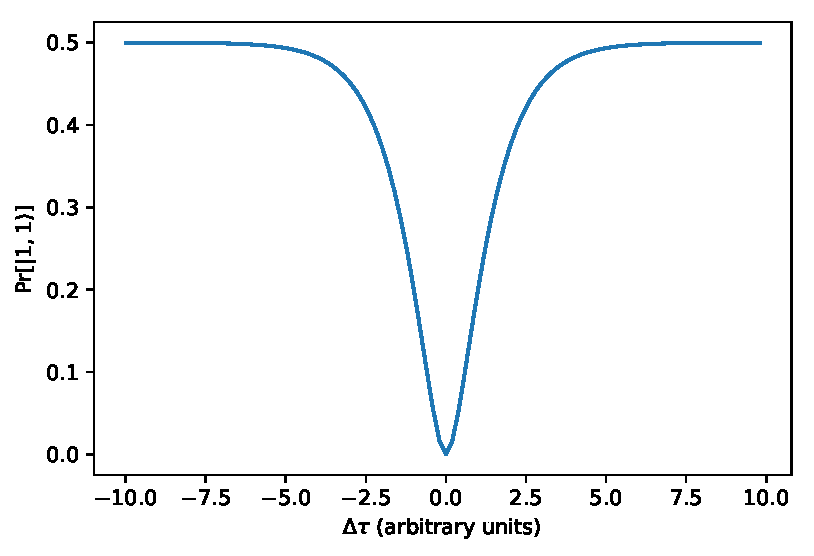
\includegraphics[width=0.5\linewidth]{preliminary_bs/hom_plot}
\end{center}
\caption{\label{fig:hom-plot}The probability of seeing the coincident $\ket{1,1}$ output from a Hong-Ou-Mandel experiment over $\Delta\tau$.}
\end{figure}

If we only measure what spatial mode our photons are in and discard the wavelength, we will find that we are in the Fock state $\ket{2,0}$ with probability $v^2/2 + d^2/4$ and likewise for $\ket{0,2}$, but we'll also find ourselves in the state $\ket{1,1}$ with probability $d^2/2$. Noting that $d^2 = 1-v^2$ and that $v=e^{-\Delta\tau}$ for some $\Delta\tau\in \mathbb{R}$ such that $\Delta\tau \geq 0$, it is easy to see that adjusting $\Delta\tau$ determines how likely we are to see coincidences at the output: if $\Delta\tau=0$, meaning that our photons are completely indistinguishable, we don't see any coincidences at all; as $\Delta\tau\rightarrow\pm\infty$, corresponding to completely distinguishable photons, then we see coincidences with probability 1/2. This is where the ``dip'' in Hong-Ou-Mandel Dip comes from: as our photons become more indistinguishable we see a drop in coincidences. This is plotted visually in Figure \ref{fig:hom-plot}. The extent to which we see a dip is known as the visibility of a Hong-Ou-Mandel dip, hence $v$, and is a standard technique when characterising linear optics experiments to determine how distinguishable pairs of photons are. Physically, $\Delta\tau$ corresponds to the difference between our photons, for example if there is a difference in path length between the photon sources and the beamsplitter.

In first quantisation, we can likewise realise this interference by introducing a second register noting what Label mode our photons are in. Our state is now

\begin{equation}
\ket{\psi} = \frac{1}{\sqrt{2}}\left(v(\ket{12}+\ket{21})\ket{RR}+d(\ket{12}\ket{RG} + \ket{21}\ket{GR})\right).
\end{equation}

Our unitary $U$ will act as $U\otimes U$ on the spatial modes and $I\otimes I$ on the Label modes. Thus, our state evolves to

\begin{align}
U^{\otimes 2}\otimes I^{\otimes 2}\ket{\psi} &= \frac{v}{2\sqrt{2}}\left((2i\ket{11}+(1+i^2)\ket{12}+(i^2+1)\ket{21}+2i\ket{22})\ket{RR}\right)\nonumber\\
&\quad+\frac{d}{2\sqrt{2}}\left(i\ket{11}(\ket{RG}+\ket{GR})+i\ket{22}(\ket{RG}+\ket{GR})\right)\nonumber\\
&\quad+\frac{d}{2\sqrt{2}}\left(\ket{12}(\ket{RG}-\ket{GR})+\ket{21}(\ket{GR}-\ket{RG})\right)\\
&= \frac{iv}{\sqrt{2}}\left((\ket{11}+\ket{22})\ket{RR}\right)\nonumber\\
&\quad+\frac{d}{2\sqrt{2}}\left(i(\ket{11}+\ket{22})(\ket{RG}+\ket{GR})+(\ket{12}-\ket{21})(\ket{RG}-\ket{GR})\right).
\end{align}

Again, we see that coincidences occur with probability $d^2/2$, matching the first quantisation result.

A rich library of theoretical work has been developed on the topic of Boson Sampling under distinguishability in recent years \cite{rohde2015, shchesnovich2015, tichy2015, tamma2016nonidentical, menssen2017}. Here, we shall follow the notation of Tichy \cite{tichy2015}, but note that this model of distinguishability is equivalent to several of the other models also mentioned. Tichy uses an $m\times m$ Gram matrix $\mathcal{S}_{i,j}$ to discribe the indistinguishability between photons generated in mode $i$ and photons generated in mode $j$, noting that any pair of photons generated in the same mode are indistinguishable from one another. Under Tichy's model, the probability of outcome $\ket{S'}$ is

\begin{equation}
\prob[S'] = \sum_{\sigma\in\symm_n}\prod_{i=1}^n\mathcal{S}_{i,\sigma(i)}\per(U_{S',S}*U_{S',\sigma(S)}^*),
\label{eqn:tichy-perm}
\end{equation}

\noindent where $*$ denotes element-wise multiplication, $M^*$ is the matrix whose elements are complex conjugates of $M$, and $\sigma(S)$ means the elements of $S$ permuted by $\sigma$. Again, the Hong-Ou-Mandel Dip can be visualised in this instance by noting that $\mathcal{S}_{1,2} = \mathcal{S}_{2,1} = v$:

\begin{align}
\prob[(1,1)] &= \per\begin{pmatrix}\frac{1}{\sqrt{2}}\times\frac{1}{\sqrt{2}}&\frac{i}{\sqrt{2}}\times\frac{-i}{\sqrt{2}}\\\frac{i}{\sqrt{2}}\times\frac{-i}{\sqrt{2}}&\frac{1}{\sqrt{2}}\times\frac{1}{\sqrt{2}}\end{pmatrix} + v^2 \per\begin{pmatrix}\frac{1}{\sqrt{2}}\times\frac{-i}{\sqrt{2}}&\frac{i}{\sqrt{2}}\times\frac{1}{\sqrt{2}}\\\frac{i}{\sqrt{2}}\times\frac{1}{\sqrt{2}}&\frac{1}{\sqrt{2}}\times\frac{-i}{\sqrt{2}}\end{pmatrix}\\
&= \per\begin{pmatrix}\frac{1}{2}&\frac{1}{2}\\\frac{1}{2}&\frac{1}{2}\end{pmatrix} + v^2 \per\begin{pmatrix}\frac{-i}{2}&\frac{i}{2}\\\frac{i}{2}&\frac{-i}{2}\end{pmatrix}\\
&= \frac{2-2v^2}{4}\\
&= \frac{1-v^2}{2}\\
&= \frac{d^2}{2},
\end{align}

\noindent matching the result discussed above.

So what can be done to work around distinguishability? A few options are available. Shchesnovich used average mutual fidelity to give an upper bound on the complexity, stating that a sampling experiment is more powerful when the single-photon mode mismatch scales as $O(n^{-3/2})$ for $n$ photons~\cite{shchesnovich2014}. Rohde and Ralph \cite{rohde2012} suggest applying filtering to discard photons which are too distinguishable. This does end up creating loss as a result, trading one imperfection for another, but this can be tolerable to some extent, as we shall see in Section \ref{ssec:imperfections-loss} \cite{rohde2012, aaronson2016}. Another option, known as Multi-Boson Correlation Sampling \cite{tamma2014, tamma2015, laibacher2015, tamma2016, laibacher2017}, is to measure across some of these characteristics in such a way that the photons end up essentially behaving indistinguishably. Laibacher and Tamma used an example where $n$ photons were of different colours, and showed that a suitable time interval and polarisation could be chosen such that at the detectors the photons appeared indistinguishable. This was later demonstrated experimentally by Wang et al.~\cite{wang2018timebin}, as well as a subsequent experiment by Orre et al.~\cite{orre2019} where frequency-resolving detectors were used to demonstrate Boson Sampling with photons generated at different time.

Finally, we note there are a number of results that link distinguishability in linear optics to representation theory \cite{adamson2008, deguise2014, turner2016, menssen2017, stanisic2018}. We will introduce representation theory in Section \ref{sec:sw-duality}, and explain its link to Boson Sampling in more detail in Chapter \ref{chp:noisy_circuit}.

\subsection{Loss}
\label{ssec:imperfections-loss}

Now we turn to photon loss, where we know that some photons were generated at the input but not detected at the output. There are a wide variety of reasons for why loss might occur, including but not limited to coupling between optical components, two-photon absorption, Rayleigh scattering and detector inefficiencies \cite{silverstone2016, rosenfeld2019}. Note that unlike distinguishability, here we will discuss two different ways of modelling photon loss, based on first and second quantisation, respectively.

First, we shall look at the model of photon loss in second quantisation, otherwise known as the ``beam splitter'' model \cite{oszmaniec2018, garciapatron2017, brod2019}. In this model, loss is induced by adding ``lost'' modes $a_{\textrm{L},i}^\dagger$ to our experiment. These additional modes are coupled to spatial modes in our experiment by a single beam splitter with transmission $\sqrt{\eta}$ for some $\eta \in [0,1]$

\begin{equation}
a_1^\dagger \rightarrow \sqrt{\eta} a_1^\dagger + \sqrt{1-\eta}a_{\textrm{L}, i}^\dagger
\end{equation}

\noindent such that a photon which starts in this spatial mode ends up in our lost mode with probability $1 - \eta$. The fact that only a single beam splitter couples this additional mode to a spatial mode in our experiment is required to ensure that any photons which are lost do not reappear later in the experiment. Finally, these additional spatial modes are traced out to induce the photon loss

\begin{align}
\trace_{\textrm{L}}[a_1^\dagger\ket{0,0_{\textrm{L}}}] &\rightarrow \trace_{\textrm{L}}[(\sqrt{\eta}a_1^\dagger + \sqrt{1-\eta}a_{\textrm{L}}^\dagger)\ket{0,0_{\textrm{L}}}]\\
&= \trace_{\textrm{L}}[\sqrt{\eta}a_1^\dagger\ket{0,0_{\textrm{L}}} + \sqrt{1-\eta}a_{\textrm{L}}^\dagger\ket{0,0_{\textrm{L}}}]\\
&= \trace_{\textrm{L}}[\sqrt{\eta}\ket{1,0_{\textrm{L}}} + \sqrt{1-\eta}\ket{0,1_{\textrm{L}}}]\\
&= \eta\ket{1}\bra{1} + (1-\eta)\ket{0}\bra{0}.
\end{align}

At first glance, it might seem like this model of loss might require an arbitrarily large number of additional spatial modes, due to the requirement that each loss-inducing beam splitter couples to an additional spatial mode. However, note that if we have two loss-inducing beam splitters in sequence with survival probabilities $\eta_1$ and $\eta_2$, respectively, then this is equivalent to a singe loss-inducing beam splitter with overall survival probability $\eta_1\eta_2$. This reduces the number of additional modes required to a number polynomial in terms of how many optical components are in our experiment. As shown in Section \ref{ssec:universal-lo}, this number is polynomial in $m$ and $n$. It is in fact possible to reduce this number of additional modes even further, in cases where the loss-inducing components can commute with the optical components in an experiment. As we will see in Section \ref{ssec:simulating-lossy-bs}, this is often used to approximate a lossy linear optical interferometer as a single layer of loss followed by a less lossy interferometer.

We now move to the model of photon loss in first quantisation. Note that the beam splitter model considered above is inconvenient in first quantisation due to the fact that it is tracing out spatial modes, which is not easily done in first quantisation. Likewise, this next model, which can be seen as tracing out particles, is inconvenient in second quantisation.

Consider a Boson Sampling experiment which starts with $n$ photons, of which only $k$ are detected. Crucially, not only does loss reduce the number of photons, but also we do not know which of the photons have been lost. In first quantisation, this is equivalent to performing Boson Sampling with input given by the mixed state

\begin{equation}
\rho = \sum_{\substack{K \subseteq S\\|K| = k}}p_{K}\rho_K,
\end{equation}

\noindent where $\rho_K$ describes a photonic input state with $k$ photons whose spatial modes are specified by $K$. When this loss is uniform, meaning that $p_K=1/\binom{n}{k}\forall K$, this is equivalent to tracing out $n-k$ particles \cite{oszmaniec2018}. This leads to the probability distribution forming a convex sum over different subsets of input photons

\begin{equation}
\prob[K'] = \sum_{\substack{K \subseteq S\\|K| = k}}p_{K}|\per(U_{K',K})|^2,
\end{equation}

\noindent where $p_K$ is the probability of the photons which started in input modes $K$ surviving, with $\sum_Kp_K = 1$.

One known complexity result is by Aaronson and Brod \cite{aaronson2016}, who considered Boson Sampling with uniform loss. Aaronson and Brod showed that in this model, Boson Sampling remains classically hard if $k=n-\ell$ for some constant $\ell$. This was proven by showing that if someone could estimate a convex sum of squared permanents of submatrices of an $(n)\times(n)$ matrix, then one can estimate the squared permanent of an $(n-\ell)\times(n-\ell)$ matrix with bounded probability. However, this only works if a constant number of photons are lost, regardless of how large $n$ is. No hardness proofs exist even for the case of a constant fraction of photons being lost.

Another workaround for loss was suggested by Latmiral, Spagnolo and Sciarrino \cite{latmiral2016}. This proposal considers Scattershot Boson Sampling under photon loss. This is a sensible proposal, as the point of Scattershot Boson Sampling is to use a large number of photon sources to produce a small number of photons at the output. However, one weakness is that there is now a chance of a photon not being heralded, as the photon measured to detect its presence might be lost. Latmiral, Spagnolo and Sciarrino propose working around this by placing a shutter on each input mode, such that only heralded photons can enter the interferometer. From analysis of the distribution under this new architecture, Latmiral, Spagnolo and Sciarrino gave bounds for how long it would take to simulate lossy Scattershot Boson Sampling, tough it is important to note that the classical algorithm used was to compute the probability of every single outcome and then sample over the full probability distribution. For this na\"ive sampling strategy, Latmiral, Spagnolo and Sciarrino showed that as few as 7 photons across 50 modes would be sufficient for a quantum advantage, but there are far more efficient classical algorithms as we will see in Section \ref{sec:classical-simulations}.

Two papers have experimentally explored Boson Sampling under loss. The first, in 2018 by Wang et al.~\cite{wang2018}, considers five, six and seven photon Boson Sampling with one and two photons lost. The second, as mentioned in Section \ref{sec:experimental-achievements}, was performed in 2019 by Wang et al.~\cite{wang2019}, and demonstrates Boson Sampling with 20 input photons of which up to 14 survive.

\subsection{Other Imperfections}

Before we move on to classical simulations, we will briefly mention here other imperfections that might occur or be considered in a Boson Sampling experiment, as well as what results are known for these models.

\subsubsection{Errors in the interferometer implemented}

It is not necessarily possible to implement a random unitary $U$ perfectly in an interferometer. Even when using universal linear optical interferometers such as those mentioned in Section \ref{ssec:universal-lo}, an interferometer might require us to apply a phase shift that our electronic components are not fine-grained enough to implement. There may also be other component imperfections, such as a beam splitter which is not perfectly balanced.

The complexity of Boson Sampling when our interferometer is not implemented perfectly was first considered by Leverrier and Garc\'{a}a-Patr\'{o}n \cite{leverrier2015}. Let $U$ be our ideal unitary, and $\tilde{U}$ be the unitary actually implemented by our interferometer. Leverrier and Garc\'{a}a-Patr\'{o}n showed that it is necessary for each optical component to have fidelity $1-O(1/n^2)$ in order for the probability of an outcome $S'$ under $\tilde{U}$ to be approximately close to the probability of the same outcome under $U$. Arkhipov \cite{arkhipov2015} improved this result, showing that it is sufficient for each optical component to be implemented up to $O(\epsilon/n^2\log m)$ error in order for the $L_1$ distance between the distributions generated by $U$ and $\tilde{U}$ to be at most $\epsilon$. Note that this result by Arkhipov uses the $O(n\log m)$-depth interferometer mentioned in Section \ref{ssec:universal-lo}; for other universal interferometers \cite{hurwitz1897, reck1994, clements2016}, a smaller component-wise error might be required.

It is interesting to note that a constant error in each optical component is not sufficient for Boson Sampling, and that instead the component-wise error must decrease as $m$ and $n$ increase. Arkhipov argues that this is unsurprising; each photon interacting with the interferometer induces some error, and as the size of the unitary grows so too must the number of optical components.

\subsubsection{Low depth interferometers}

Loss is more likely to occur in Boson Sampling if the interferometer has a high depth. An intuitive question to ask in this case is what can be done with a Boson Sampling circuit of reduced depth? A hardness proof for exact sampling was given Brod \cite{brod2015}, showing that even four layers of beam splitters was sufficient to ensure hardness in the exact case. Classical algorithms for these instances were later devised, by taking advantage of the low depth to only simulate interference between photons which could actually cross paths \cite{deshpande2018, maskara2019}. Note that these classical simulation algorithms inherently assume the photons are not all generated adjacently from each other.

\subsubsection{Dark counts}

Dark counts occur when a detector registers a photon even though one was not present. This is most often due to thermal noise within the single photon detector, meaning that even if the detector was in complete darkness it would still claim that photons were present.

Dark counts themselves are not much of a challenge in Boson Sampling experiments; superconducting nanowire single photon detectors have sufficiently low dark counts that false clicks can be noticed easily and the experiment discarded \cite{kitaygorsky2005}. However, where they become challenging is when loss is also involved: It is very difficult to differentiate between a photon not being lost and a photon being lost combined with a false click at the detector. The intersection of these two imperfections was considered by Shchesnovich \cite{shchesnovich2014darkcounts}, who showed that both dark counts and loss can be considered as producing additive errors with respect to $m$ and $n$.

\subsubsection{Gaussian noise}

A Gaussian noise model was proposed as a way of considering errors in Boson Sampling by Kalai and Kindler \cite{kalai2014}. In this model, the probability of an outcome $S'$ is still related to the permanent of a matrix, but now  the matrix in question is $\sqrt{1-\epsilon}U_{S',S}+\sqrt{\epsilon}X$ for some Gaussian matrix $X$ that acts as our noise. Kalai and Kindler suggest that for $\epsilon=\omega(1/n)$, vanilla Boson Sampling and Boson Sampling under Gaussian noise are already uncorrelated, and furthermore for $\epsilon = \Omega(1)$, that the probability of an outcome of Boson Sampling under Gaussian noise can be approximated by up to constant error.

\section{Classical Simulation Algorithms}
\label{sec:classical-simulations}

Having introduced distinguishability and loss, we are now ready to discuss classical simulation algorithms for these imperfections. We will start by explaining classical algorithms for vanilla Boson Sampling, which were the original classical simulators devised. We will then discuss Boson Sampling under fully distinguishable photons, as well as Boson Sampling under various models of loss. Finally, we shall consider the classical simulation algorithms of \cite{renema2018, renema2018loss}, which were the first known classical algorithms to consider both distinguishability and loss.

\subsection{Simulation algorithms for ideal Boson Sampling}

Boson Sampling under ideal conditions (lossless indistinguishable single photons) is intractable for sufficiently large $n$. 
Until recently the only classical simulation method explicitly known was to compute the entire probability distribution before taking a sample, though it was widely believed that more efficient, albeit still exponential time, approaches existed. 
A brute force method cannot scale, due to both the number of possible outcomes and the complexity of computing even one $n\times n$ complex matrix permanent.

Two major results gave the first explicit classical simulation strategies which were faster than brute-force sampling. 
The first, by Neville et al.~\cite{neville2017}, demonstrated that Boson Sampling experiments with up to 30 photons could be simulated on a single laptop, and suggests that a supercomputer could handle up to 50 photons. 
This was achieved by starting with the classical distribution of $n$ distinguishable photons, and then using Metropolised Independence Sampling to adapt the distribution to that of ideal Boson Sampling.
The second result, by Clifford \& Clifford \cite{clifford2017}, gave a classical algorithm for exact Boson Sampling and runs in time equivalent to computing two $n \times n$ matrix  permanents per sample with a polynomial overhead. 
This is through a combination of optimizations, particularly computing marginal probabilities and sampling via the chain rule.

\subsection{A simulation algorithm for fully distinguishable Boson Sampling}
\label{ssec:fully-dist-sim}

In the case where the $n$ input photons are fully distinguishable, a simple polynomial time algorithm exists \cite{aaronson2014}. In this case, there is no photon interference, so photons can be sampled individually. This is done by taking a photon which starts in mode $i$, and sampling output mode $j$ with probability $|U_{j,i}|^2$. Repeating for all photons gives us the complete sample in $O(mn)$ time.

\subsection{Simulation algorithms for Boson Sampling with loss}
\label{ssec:simulating-lossy-bs}

Another common source of imperfections in linear optics is that of photon loss, which arises through a number of different means. 
Indeed, any large-scale demonstration of Boson Sampling is bound to face photon loss, and therefore needs to take such issues into account. 
Some results have already shown instances where hardness is still retained, such as when only a constant number of photons are lost \cite{aaronson2016,wang2018}.

Neville et al.\ compared the classical simulation of their approach to a Boson Sampling experiment where any photon loss was considered a rejected experiment \cite{neville2017}. Novel classical simulations for Boson Sampling under loss have also been considered by use of classically simulable states such as thermal \cite{garciapatron2017} or separable \cite{oszmaniec2018} states.

There has also been some consideration of how classical simulations can be generalised to non-uniform loss. 
This usually means photon loss that is dependent on the number of optical components, with each component having transmission probability $\tau$. 
Classical simulation methods can be generalised to this model by identifying a layer of uniform losses from the circuit, followed a non-uniform lossy circuit which can be simulated classically through the use of additional modes for lost photons \cite{garciapatron2017,oszmaniec2018}. 
These results showed that Boson Sampling under non-uniform loss can be classically simulated as long as every photon encounters at least $O(\log n)$ components. More recently, Brod and Oszmaniec developed on these methods to give a polynomial-time algorithm in the case where some photons experience little or no loss while others experience significant amounts of loss, by extracting losses into a layer of non-uniform loss and simulating via a generalisation of the Clifford \& Clifford algorithm \cite{brod2019}.

\subsection{Simulation under multiple imperfections}
\label{sec:renema-review}

In \cite{renema2018, renema2018loss}, Renema et al.\ consider the Tichy model of inter-photon distinguishability described in Section \ref{ssec:imperfections-distinguishability}. 
The probability distribution of arbitrarily distinguishable bosons is modelled as
\begin{equation}
\prob[S'] = \sum_{\sigma\in\symm_n}\prod_{i=1}^n\mathcal{S}_{i,\sigma(i)}\per(M*M^*_{1,\sigma}) ,
\end{equation}
where $\mathcal{S}$ is the same matrix describing the distinguishability as in the previous section, $M$ is a matrix defined by the rows and columns of our interferometer $U$ selected based on our photon output $S'$ and input $S$, $M^*_{1,\sigma}$ is the conjugate matrix with the identity permutation applied to rows and permutation $\sigma$ applied to columns, and $*$ denotes element-wise multiplication. 
They further restrict to a model where the indistinguishability overlap is defined by a single parameter $\mathcal{S}_{i,j} = x + (1-x)\delta_{i,j}, x \in [0,1]$.
The sum over permutations can be ordered based on how many \emph{fixed points} a permutation has, giving
\begin{equation}
\prob[S'] = \sum_{j=0}^n\sum_{\sigma^j}x^j\per(M*M^*_{1,\sigma}) , \label{eqn:renema-state}
\end{equation}
where $\sigma^j$ denotes permutations which have $n-j$ elements as fixed points.
Each permanent can be broken down via the Laplace expansion into a sum of a complex matrix permanent multiplied by a positive matrix permanent:
\begin{equation}
\prob[S'] = \sum_{j=0}^n\sum_{\sigma^j}x^j\sum_{\substack{J'\leq S'\\|J'|=j}}\per(M_{J',1}*M^*_{J',\sigma_p})\per(|M_{\bar{J'},\sigma_u}|^2) ,
\end{equation}

\noindent where $J'$ is an occupation with $j$ photons. Here we are now choosing submatrices of $M$, with $J'$ representing the $\binom{n}{j}$ possible combinations of rows from $M$, $\bar{J'}$ representing the remaining rows, and $\sigma_p$ and $\sigma_u$  representing permuted and unpermuted elements of $\sigma$ respectively.
The $J' \leq S'$ notation is used to indicate that $J'$ is a Fock state such that $J_i\leq S'_i \,\forall i\in[m]$.

The classical simulation method used truncates the number of non-fixed points in a permutation as being at most $k$, with the remainder of the probability treated as an error margin. 
It is important to note while these approximations are real, they are not necessarily positive. 
This is due to the truncation, where positive higher order terms which would have corrected the probability to be positive are now missing from the approximation. 
To correct this, any negative approximations are rounded up to $0$.
These probabilities are then used to train a Metropolised Independence Sampler, akin to the technique of \cite{neville2017}. 
Training this sampler requires approximating a number of probabilities dependent on the underlying distribution, each of which involves computing $O(n^{2k})$ permanents of $k\times k$ complex matrices, and the same number of permanents of $(n-k)\times (n-k)$ matrices with non-negative entries. 
The permanents of $k\times k$ complex matrices can be computed classically in $O(k2^k)$ time via Ryser's algorithm, and the permanents of matrices with non-negative entries can be approximated up to multiplicative error in polynomial time \cite{jerrum2004,huber2008}. 
As long as $k$ is independent of $n$, this means that there is a polynomial runtime.

To work out a suitable value $k$, define coefficients $c_j$ as

\begin{equation}
c_j = \sum_{\sigma^j}\sum_{\substack{J'\leq S'\\|J'|=j}}\per(M_{J',1}*M^*_{J',\sigma_p})\per(|M_{\bar{J'},\sigma_u}|^2)\label{eqn:coefficients}.
\end{equation}

Assuming the matrices are Gaussian, the variance of each permanent can be bounded as

\begin{equation}
\var[\per(M_{J',1}*M^*_{J',\sigma_p})] = \frac{j!}{m^{2j}},
\end{equation}
and
\begin{equation}
\var[\per(|M_{\bar{J'},\sigma_u}|^2)] < \frac{(n-j)!}{m^{2(n-j)}}\sum_{l=0}^{n-j}\frac{1}{l!}.
\end{equation}

This leads to two key results. The first is that the variance of $c_j$ tends towards a constant value:
\begin{align}
\var[c_j] &< \left(\frac{n!}{m^n}\right)^2\frac{1}{e}\sum_{l=0}^{n-j}\frac{1}{l!} \label{eqn:var}\\
&\rightarrow\left(\frac{n!}{m^n}\right)^2 \textrm{ as } n\rightarrow\infty,
\end{align}
and the second is that the covariance for different values of $j$ is zero:
\begin{equation}
\cov[c_j,c_j'] = 0\, \forall\, j\neq j'\label{eqn:covar}.
\end{equation}
From this one can approximate the variance of the error as a geometric series, which as $n\rightarrow\infty$ tends towards the inequality
\begin{align}
\var[\Delta \prob[S']] &= \var[\prob[S']-\prob_k[S']]\\
&= \sum_{j=k+1}^nx^{2j}\var[c_j]\label{eqn:renema-variance}\\
&< \left(\frac{n!}{m^n}\right)^2\left(\frac{x^{2(k+1)}}{1-x^2}\right),
\end{align}
\noindent where $P_k$ is the probability distribution when truncated at $j\leq k$ for some $k<n$.

Finally one can use a Markov inequality to show that if the variance of the error is of the form $(n!/m^n)^2\epsilon^2$, the average error of the simulation is at most $\epsilon$ \cite{renema2018loss}.
Crucially, this value of $\epsilon$ is only dependent on $x$ and $k$ and no longer dependent on $n$.
This means that for any value of $x$, one can choose a suitable value of $k$ to achieve a required error $\epsilon$, and run a classical simulation in time polynomial in $n$.

In \cite{renema2018loss}, the method described above was adapted to consider uniform loss as well as distinguishability, showing that the same result can be found, with the only difference being that $x$ is now replaced by $\alpha=\sqrt{\eta}x$, where $\eta$ is the probability of each individual photon surviving. 
Crucially, this result demonstrated that Boson Sampling where a constant fraction of photons were lost can be simulated in $O(\ell^{2k}k2^k)$, where $\ell$ is the number of photons which survive and $k$ is only dependent on the constant $\ell/n$, distinguishability $x$, and the desired accuracy of the simulation. 
This can be expanded to classically simulating Boson Sampling under uniform loss by sampling $\ell$ from the binomial distribution before sampling output photons, which offers a runtime of $O(n^{2k}k2^k)$. 

Although this runtime is polynomial in terms of $n$ and can therefore be considered asymptotically efficient, it might not be classically simulable in practice. 
There are three main contributions to this: 
First, the algorithm is reliant on Metropolised Independence Sampling, which potentially requires many probabilities to be approximated per sample. 
Second, approximating each probability requires $O(n^{2k})$ permanents of $k\times k$ matrices, which even for small $k$ could be a large number of permanents. 
And third, approximating each probability requires $O(n^{2k})$ permanents of $(n-k)\times(n-k)$ matrices with non-negative elements. 
Although approximating permanents of matrices with non-negative elements can be achieved in polynomial time, classical algorithms still have a runtime ranging from $O((n-k)^4\log(n-k))$ to $O((n-k)^{7}\log^4(n-k))$, depending on the sparsity of the matrix~\cite{huber2008}. These issues are the main points to address in order to achieve a practical classical algorithm for Boson Sampling. The Clifford \& Clifford algorithm could help to alleviate these issues, but there is a challenge due to the fact that the approximation used in Renema et al.\ does not correspond to a bosonic state. 
This in turn leads to negative probabilities, which are not clear how to correct for in the Clifford \& Clifford algorithm.

\section{The Schur-Weyl Duality}
\label{sec:sw-duality}

We'll now turn to the Schur-Weyl Duality, a theorem related to the irreducible representations of the symmetric and unitary groups. Although this seems like a sudden jump in subject, we emphasise to the reader that the connection between linear optics and Boson Sampling as described earlier in this chapter and the Schur-Weyl Duality will be explained in Chapters \ref{chp:noisy_circuit} and \ref{chp:classical_sim}.

We will start by introducing representation theory, before explaining the Schur-Weyl Duality in detail. At the end of this section we shall consider its connection to quantum information, and in Chapter \ref{chp:noisy_circuit} how it is linked to Boson Sampling specifically. For further reading we direct the reader to \cite{fulton2004, harrow2005}.

\subsection{Representation theory}

Let $G$ be a group and $X$ a set. We define an action of $G$ on $X$ as a map $\Phi\colon G\times X \rightarrow X$ such that the action of the identity element $e\in G$ is the identity map, $\Phi_e(x) = \Phi(e, x) = x$, and the following relation holds:

\begin{equation}
\Phi_{g_1}(\Phi_{g_2}(x)) = \Phi_{g_1g_2}(x).
\end{equation}

One example is the action of the permutation group $S_n$ on the set of numbers from 1 to $n$, defined as $\Phi_\sigma(i) = \sigma^{-1}(i)$. Note that $\Phi$ need not be injective with respect to $G$, so another trivial example is the identity action, which is $\Phi_g(x) = x \forall g \in G$.

A representation is defined as a vector space $V$ combined with an action $\Phi: G \times V \rightarrow V$ with the additional constraint that $\Phi$ is a linear map over $V$:

\begin{equation}
\Phi(g, u+v) = \Phi(g, u) + \Phi(g, v).
\end{equation}

Now let $W \subseteq V$ be a vector subspace. We say that $W$ is invariant with respect to the action of $\{\Phi_g\colon g\in G\}$ if

\begin{equation}
\Phi_g(w) \in W \forall g \in G, w \in W.
\end{equation}

Two trivial example of invariant subspaces are the full vector space $W=V$ and the empty vector space $W=\{0\}$. We call a vector subspace $W$ invariant if the above holds and $W$ is not equal to $V$ or $\{0\}$.

This finally brings us to the topic of irreducible representations. A representation $V, \Phi$ of $G$ is irreducible, also known as an irrep, if it contains no proper invariant subspaces. If $V$ does contain a proper invariant subspace, then we say that $V$ is reducible.

\subsection{Symmetric and Unitary Groups}

The main interest of this thesis is the representation theory of the unitary group U$(m)$, and its action on the space of $(\mathbb{C}^{m})^{\otimes n}$. The intuition for linking this to Boson Sampling is that each vector in $\mathbb{C}^m$ is referring to a photon which could be in one of $m$ modes, and the action of $U \in \unitary(m)$ will be our interferometer.
As we shall see from the Schur-Weyl Duality, the irreducible representations for $\unitary(m)$ are intimately related to those of the symmetric group $\textrm{S}_n$.

For the tensor space of $(\mathbb{C}^{m})^{\otimes n}$, the actions of the symmetric and unitary groups on a tensor $v_1\otimes\dots\otimes v_n \in (\mathbb{C}^m)^{\otimes n}$ are explicitly as follows. 
For a permutation $\sigma \in \textrm{S}_n$, the action permutes the tensor factors,

\begin{equation}
\Phi_\sigma(v_1\otimes\dots\otimes v_n) = v_{\sigma^{-1}(1)}\otimes\dots\otimes v_{\sigma^{-1}(n)},
\end{equation}

\noindent and for a unitary matrix $U \in \textrm{U}(m)$, the action is the $n$-fold tensor product $\Phi_U = U^{\otimes n}$.

It is a simple exercise to see that these two actions commute:

\begin{align}
\Phi_U(\Phi_\sigma(v_1\otimes\dots\otimes v_n)) &= \Phi_U(v_{\sigma^{-1}(1)}\otimes\dots\otimes v_{\sigma^{-1}(n)})\\
&= (Uv_{\sigma^{-1}(1)})\otimes\dots\otimes(Uv_{\sigma^{-1}(n)})\\
&= \Phi_\sigma((Uv_1)\otimes\dots\otimes (Uv_n))\\
&= \Phi_\sigma(\Phi_U(v_1\otimes\dots\otimes v_n)).
\end{align}

The Schur-Weyl Duality describes how $(\mathbb{C}^m)^{\otimes n}$ can be decomposed into irreps for the direct product group $\unitary(m)\times\symm_n$.

\begin{theorem}[Schur-Weyl Duality~\cite{rowe2012}]
\label{thm:schur-weyl-duality} The complex vector space of $(\mathbb{C}^m)^{\otimes n}$ decomposes into irreducible subspaces
\begin{equation}
(\mathbb{C}^m)^{\otimes n} \simeq \bigoplus_{\lambda\vdash n} \mathbb{C}^{\{\lambda\}} \otimes \mathbb{C}^{(\lambda)} ,
\end{equation}
where $\mathbb{C}^{\{\lambda\}}$ carries irrep $\{\lambda\}$ of $\textrm{U}(m)$ and $\mathbb{C}^{(\lambda)}$ carries irrep $(\lambda)$ of $\textrm{S}_n$, and $\simeq$ indicates a change of basis is involved.
The dimension of irrep $(\lambda)$ can be viewed as the multiplicity of irrep $\{\lambda\}$, and vice versa.
\end{theorem}

It is common to label irreps of both of these groups by ordered partitions $\lambda = (\lambda_1,\lambda_2,\cdots,\lambda_m)$ of $n$ such that $\lambda_i \geq \lambda_{i+1}$ and $\sum_{i = 1}^m \lambda_i = n$.
We usually suppress zeros in this notation, so for example the totally symmetric irrep $\lambda=(n, 0,\dots,0)$ is written $(n)$. 
The number of nonzero $\lambda_i$ is called the length of the partition, $\ell(\lambda)$, and only partitions with $\ell(\lambda) \leq m$ occur, which we will assume in all of our expressions that follow. Similarly, the width of the partition is $w(\lambda) = \lambda_1$, the largest partition in $\lambda$.
%Following the convention of~\cite{rowe2012}, we shall label irreps of S$_n$ and U$(m)$ indexed by $\lambda$ as $(\lambda)$ and $\{\lambda\}$, respectively.

\subsection{The Quantum Schur Transform}
\label{ssec:quantum-schur-transform}

The Quantum Schur Transform realises the basis change of The Schur-Weyl Duality as a quantum circuit. This circuit takes as input a state in the basis $(\mathbb{C}^m)^{\otimes n}$, and decomposes it into a basis of states labelled by which irrep $\lambda$ they are in.

The canonical example of the Quantum Schur Transform is when $m=n=2$. In this case, the only partitions available are $\lambda=(2,0)$ and $\lambda=(1,1)$. Our representation labelled by $\lambda=(2,0)$ is defined by the basis states $\ket{00}$, $\ket{11}$ and $(\ket{01}+\ket{10})/\sqrt{2}$, while our $(1,1)$ irrep is simply the state $(\ket{01}-\ket{10})/\sqrt{2}$. This is equivalent to the triplet and singlet states of two electrons and their corresponding description in angular momentum notation:

\begin{align}
\ket{j=1,m=1} &= \ket{00},\\
\ket{j=1,m=0} &= \frac{\ket{01}+\ket{10}}{\sqrt{2}},\\
\ket{j=1,m=-1} &= \ket{11},\\
\ket{j=0,m=0} &= \frac{\ket{01}-\ket{10}}{\sqrt{2}}.
\end{align}

This can generalise further to describe $n$ qubits, noting that $j=(\lambda_1-\lambda_2)/2$. The Quantum Schur Transform is even more general, offering a mapping for any collection of $m$-level qudits. Given a state $|\Psi\rangle \in (\mathbb{C}^m)^{\otimes n}$ written in the computational basis, the Quantum Schur Transform, which we denote as the quantum circuit $W$, performs the transformation
\begin{equation}
W|\Psi\rangle
 = \sum_{\lambda \vdash n} \, \sum_{q_{\lambda}} \, \sum_{p_\lambda}C^\lambda_{q_\lambda,p_\lambda}|\lambda\rangle|q_\lambda\rangle|p_\lambda\rangle , 
\end{equation}
where $\lambda$ indexes the irrep, $q_\lambda$ and $p_\lambda$ index bases of irreps $\{\lambda\}$ and $(\lambda)$ respectively, and $C^\lambda_{q_\lambda,p_\lambda}$ is a generalised Clebsch-Gordan coefficient.
For interferometry applications, the unitary action of U$(m)$ in this basis is
\begin{equation}
U : |\lambda\rangle |q_\lambda\rangle |p\rangle \rightarrow |\lambda\rangle |U\cdot q_\lambda\rangle |p\rangle := |\lambda\rangle \left( \sum_{q_\lambda'} U^\lambda_{q_\lambda, q_\lambda'} |q_\lambda'\rangle \right) |p\rangle ,
\end{equation}
where $U^\lambda$ is the irreducible unitary matrix corresponding to $U \in \mathrm{U}(m)$. Equivalently, one can write $q_\lambda$ as a photon occupation $\underline{n} \in F(\mathbb{C}^m)$ and inner multiplicity $r_{\underline{n}} \in \mathbb{N}$.

Although this notation will largely not be used in this thesis, we will briefly describe how the basis states of $\{\lambda\}$ and $(\lambda)$ are denoted. An equivalent way of writing irrep $\lambda$, rather than using partitions, is to use Young diagrams. These are diagrams of $n$ boxes across $m$ rows such that the number of boxes in row $i$ is at most the number of boxes in row $i-1$. A simple mapping from partitions $\lambda$ to Young diagrams is then that row $i$ of the diagram has $\lambda_i$ boxes. Using $m=n=3$ as an example, the possible irreps are as follows:

\begin{equation}
(3) \equiv \yng(3),
\end{equation}

\begin{equation}
(2,1) \equiv \yng(2,1),
\end{equation}

\begin{equation}
(1,1,1) \equiv \yng(1,1,1).
\end{equation}

The advantage of using Young diagrams is that they also give convenient notation for the basis states of $\{\lambda\}$ and $(\lambda)$. For $\{\lambda\}$, our unitary irreps, we use the Gelfand-Tsetlin basis. In this basis, we denote basis states by semistandard Young tableaux, which are Young diagrams with each box filled with an integer from $1,\dots,m$ such that each row is non-decreasing and each column is strictly ascending. The Gelfand-Tsetlin bases for $m=n=3$ for instance are the following:

\begin{align}
\mathbb{C}^{\{(3)\}} = &\textrm{span}\left\{\ket{\young(111)}, \ket{\young(112)}, \ket{\young(113)}, \ket{\young(122)}, \ket{\young(123)},\right.\\ 
&\left.\ket{\young(133)}, \ket{\young(222)}, \ket{\young(223)}, \ket{\young(233)}, \ket{\young(333)}\right\},
\end{align}

\begin{equation}
\mathbb{C}^{\{(2,1)\}} = \textrm{span}\left\{\left|\young(11,2)\right\rangle, \left|\young(12,2)\right\rangle, \left|\young(13,2)\right\rangle, \left|\young(11,3)\right\rangle, \left|\young(12,3)\right\rangle, \left|\young(13,3)\right\rangle, \left|\young(22,3)\right\rangle, \left|\young(23,3)\right\rangle\right\},
\end{equation}

\begin{equation}
\mathbb{C}^{\{(1,1,1)\}} = \textrm{span}\left\{\left|\young(1,2,3)\right\rangle\right\}.
\end{equation}

To index the basis states of $(\lambda)$, we can use the Young-Yagamouchi basis. This basis denotes states by standard Young tableaux, where each box is filled with numbers from $1$ to $n$ such that each integer occurs exactly once and all rows and columns are strictly ascending. The Young-Yagamouchi bases for $m=n=3$ for instance are the following:

\begin{align}
((3)) = &\left\{\ket{\young(123)}\right\},
\end{align}

\begin{equation}
((2,1)) = \left\{\left|\young(12,3)\right\rangle, \left|\young(13,2)\right\rangle\right\},
\end{equation}

\begin{equation}
((1,1,1)) = \left\{\left|\young(1,2,3)\right\rangle\right\}.
\end{equation}

Note that for the fully symmetric $(3)$ and antisymmetric $(1,1,1)$ irreps there is only one state, but for $\lambda = (2,1)$ there are two basis states. This creates a multiplicity, leading to two equivalent bases for the $(2,1)$ irrep of the Unitary group, with permutations mapping from one irrep to the other. The total dimensionality across these basis representations is

\begin{equation}
1\times 10+2\times 8 + 1\times 1 = 27,
\end{equation}

\noindent which is the same size as our computational basis $(\mathbb{C}^3)^{\otimes 3}$.

Of course, we have not stated explicitly how these basis states map to the standard basis. We shall omit these details for simplicity, but simply note that algorithms for explicitly computing these bases do exist, by starting with a highest-weighted vector in the basis and applying lowering operators to find lower-weight vectors. Explicit algorithms can be found in, for example, \cite{alex2011, dhand2015}.

\subsubsection{Efficient Quantum Circuits}

The first demonstration of an efficient quantum circuit was for $m=2$, proven in 2004 and later published in 2006 by Bacon, Chuang and Harrow \cite{bacon2004}. This circuit worked by decomposing the Schur Transform into a sequence of $n$ Clebsch-Gordan Transforms, each coupling pairs of qubits together. The individual Clebsch-Gordan transformations could then be implemented using two Controlled-Not gates and a single doubly-controlled rotation gate in the $y$-direction, which can be implemented up to precision $\epsilon$ in $O(\polylog(1/\epsilon))$ gates \cite{dawson2006, nielsen2010}. Thus, the overall runtime of this circuit was $O(n\polylog(1/\epsilon))$.

This result was subsequently generalised to arbitrary $m$ in Aram Harrow's PhD thesis \cite{harrow2005, bacon2007}. Now the Schur transform was decomposed into Clebsch-Gordan Transforms applied to pairs of qudits. The $m$-dimensional Clebsch-Gordan Transformation could be implemented efficiently by recursively applying the $(m-1)$-dimensional Clebsch-Gordan Transform followed by a reduced Wigner Transform. This Wigner Transform can, like the Clebsch-Gordan Transform for $m=2$, be implemented as two Controlled-Not Operations followed by a doubly-controlled rotation, the angles for which can be computed efficiently and for which an efficient circuit can be decomposed \cite{nielsen2010}. As a result, this circuit can be implemented in polynomial time in $m, n$ and $\log(1/\epsilon)$. Harrow also briefly mentions in a footnote that if $m \gg n$, then the runtime can be reduced to polynomial in $\log m$ by mapping to a state in $(\mathbb{C}^n)^{\otimes n}$, though this is not formally proven.

Recently there has been some interest in making this quantum circuit more efficient. Kirby and Strauch \cite{kirby2018} went into the original Bacon, Chuang and Harrow circuit for $m=2$ in more detail in order to offer a more explicit  analysis of what the quantum computer needed to do, from which they provided a number of simplifications. The result was a quantum circuit which requires $O(n^4\log(n/\epsilon))$ operators using a Clifford+$T$ gate set. They then extended this algorithm to the qudit setting, where they were able to find a circuit which uses $O(m^{1+p}n^{3m}\log^p(mn/\epsilon))$ operations from any universal set of quantum gates, where $p\approx 3.97$. Note that the number of gates grows superexponentially with $m$, due to the $n^m$ term, so while this is efficient for a constant $m$, we shall see that this circuit does not benefit our work. Another recent result by Krovi \cite{Krovi2019} gives an explicit quantum circuit which is polynomial in $n, \log m$ and $\log(1/\epsilon)$. Krovi's circuit works by first block-diagonalising the state into permutation modules, and then block-diagonalising each permutation module into irreps. Krovi argues that this circuit can be thought of as a dual  of Harrow's, as it uses the representation theory of the Symmetric Group, whereas Harrow's circuit uses that of the Unitary Group.

\subsubsection{Applications}

With efficient circuits for the Quantum Schur Transform now described, we will briefly discuss some example applications. Further applications can be found in Aram Harrow's PhD Thesis \cite{harrow2005}.

Many applications exist which simply take advantage of measuring the irreps of a quantum state. One example is estimating the spectrum of a quantum state $\rho$ from $n$ copies of the state $\rho^{\otimes n}$. Vidal et al.~\cite{vidal1999} used irreps of the Symmetric Group to find optimal measurements, that is, measurements which allow us to learn the most information about $\rho$, when we only have a fixed number of copies of $\rho$. Later, Keyl and Werner \cite{keyl2001} gave an approximator from measuring the irreps of a state, and showed that the probability of an error decreased exponentially with $n$.

Another such application is quantum state compression, the task of encoding a large quantum state in a smaller one. Hayashi and Matsumoto \cite{hayashi2002, hayashi2002simple} gave a scheme for compressing an arbitrary quantum state by weakly measuring the irrep $\lambda$ and then applying an encoding process. This scheme is variable-length, meaning that the output was not guaranteed to be bounded but the scheme would ensure that no information was lost in decoding. Hayashi and Matsumoto also showed that the probability of this scheme returning an encoded state whose size was larger than a particular bound (also known as an overflow) is optimal in terms of its exponent.

One final use, proven by Bartlett, Rudolph and Spekkens\cite{bartlett2001}, is quantum communication. One issue with communicating quantum states is that the receiver might not have the same reference frame as the sender, and so the two parties might not be working in the same basis. Bartlett, Rudolph and Spekkens gave a work-around for this, by encoding information in basis states of the Symmetric Group's irrep. A difference in reference frames will mean some unitary acting as $U^{\otimes n}$ on the communicated state, but this will only affect the irrep of the Unitary Group irrep and not the Symmetric Group where the data is actually encoded.

\subsection{Computational Complexity}
\label{ssec:schur-simulation}

We shall conclude this chapter with a discussion of known results regarding the computational complexity of the Quantum Schur Transform. In particular, we shall discuss Quantum Schur Sampling \cite{havlicek2018}, a generalisation of another model called Permutational Quantum Computing (PQC) \cite{jordan2010}, both of which have been proven to be classically simulable in many cases \cite{havlicek2019}. We will also finish with some discussion about immanants, which are a generalisation of the permanent and determinant.

We shall start by describing Permutational Quantum Computing, which was introduced by Jordan in 2010 \cite{jordan2010}. This model starts with an $n$-qubit computational basis state $\ket{x}$. The Quantum Schur Transform maps this state into the angular momentum basis, with spins coupled sequentially. This means that the spin of qubit $\ket{x_1}$ is coupled with the spin of qubit $\ket{x_2}$, the result is then coupled with the spin of $\ket{x_3}$, the result of which is then coupled with the spin of $\ket{x_4}$, and so on up to $\ket{x_n}$. After this transform is complete, a permutation is applied to reorder the spins, followed by the inverse Schur transform resulting in a new computational basis state $\ket{x'}$, which is then measured in the computational basis to produce a sample. Although computational hardness for this model was not formally proven, unlike Boson Sampling and the other models considered in Section \ref{ssec:qa-examples}, Jordan gave some reasoning for why it seems reasonable to believe that a polynomial time classical algorithm would not exist. Jordan did this by providing PQC algorithms for approximating elements of irreps of the symmetric group, as well as showing that PQC can approximately simulate certain models of Topoligical Quantum Field Theory \cite{jordan2010}. At the time of Jordan's publication, no polynomial time algorithm existed for either problem.

Quantum Schur Sampling is a generalisation of Permutational Quantum Computing, first proposed by Havl\'{i}\v{c}ek and Strelchuk, and name due to its similar structure to Quantum Fourier Sampling proposed by Fefferman and Umans \cite{fefferman2016}. In this model, rather than restricting to permutations, the circuit is free to perform any reversible classical computation on the spin qubits. The result is similar in structure to that of Shor's Algorithm, consisting of some kind of quantum transform --- Fourier for Shor's algorithm, Schur for Quantum Schur Sampling --- a polynomial-time classical circuit, and then the inverse transform and measurement. This model does not offer any (known) benefit over Permutational Quantum Computing; in fact it was first proposed not with the intention of showing further benefits, but instead to show a more general class of quantum circuit that could still be classically simulated.

It has only been in recent years that Quantum Schur Sampling has been shown to be classically simulable. This was proven as a result of two papers. The first, by Havl\'{i}\v{c}ek and Strelchuk \cite{havlicek2018}, disproved a conjecture of Jordan upon which the computational hardness of PQC was reliant: that the transition amplitudes of a PQC circuit cannot be approximated to within additive error in polynomial time. This was disproven by showing that states output from applying the Quantum Schur Transform to a computational basis state were Computationally Tractable (CT). This is a term coined by Van den Nest \cite{vandennest2011} meaning that the following tasks can be performed classically in polynomial time up to polynomial multiplicative error: first, that the amplitudes of a state can be approximated; and second, that a sample can be output from a measurement in the computational basis. With this proven for Quantum Schur Transform states, Havl\'{i}\v{c}ek and Strelchuk used a result by Van den Nest that unitary transformations which simply map between states in the same CT basis, such as permutations or reversible classical circuits in this case, will also produce a CT state. Finally, they used one more result of Van den Nest which is that the transition amplitude of two CT states can be approximated in polynomial time on a classical computer, thus rendering Jordan's conjecture false.

However, while the main claim to hardness had been proven wrong, this still left open the possibility that Quantum Schur Sampling was classically intractable. This is because while a polynomial time algorithm existed for computing the probability of an outcome, which is simply the square of the its amplitude, there might be an exponentially large number of probabilities to approximate before a sample can be obtained. This was resolved by Havl\'{i}\v{c}ek, Strelchuk and Temme, who gave a polynomial time classical algorithm for sampling when the output distribution is approximately $t$-sparse, meaning that it can be approximated by a distribution with $t$ elements with non-zero probability up to accuracy $\epsilon$. This is based on an algorithm by Schwarz and Van den Nest \cite{schwarz2013}, and follows three steps: First, they use the Computational Tractability result of \cite{havlicek2018} to show that approximate the marginal probabilities; second, they use an algorithm by Kushilevitz and Mansour to show that a subset of outcomes with high probabilities in the output distribution can be found efficiently; and third, they sample that sampling from this distribution of high-probability outcomes. Havl\'{i}\v{c}ek, Strelchuk and Temme showed that this high-probability distribution is at most $6\epsilon$ away from the Quantum Schur Sampling distribution in total variational distance and can be done in time polynomial in $n, t$ and $1/\epsilon$. But how sparse is the output of a Quantum Schur Sampling circuit? Havl\'{i}\v{c}ek, Strelchuk and Temme ran some numerical simulations exploring the output of PQC circuits with up to $n=10$ qubits, and showed that in these small cases all except $0.1\%$ of tested cases on 10 qubits could be approximated by a $2n^2$-sparse distribution up to accuracy $1/n$. Although this was not a formal proof of how many distributions are approximately sparse, it gives some intuition as to how common these sparse distributions might be.

It is also worth discussing the actions of the symmetric and unitary groups on these different representations, and how they affect the classical complexity of computing the amplitudes. For this, we shall discuss a generalisation of the matrix permanent, and known results on its complexity.

Let $\lambda$ be an irreducible representation, and $\sigma$ be a permutation. Define

\begin{equation}
\chi_\lambda(\sigma) \colon= \trace\left[\Phi_\sigma\right]
\end{equation}

\noindent as the characteristic of $\sigma$ in representation $\lambda$. Note that for any $\sigma' = \tau\sigma\tau^{-1}$ for some $\tau \in \symm_n$, $\chi_\lambda(\sigma) = \chi_\lambda(\sigma')$, meaning that $\sigma$ and $\sigma'$ are in the same conjugacy class:

\begin{align}
\chi_\lambda(\sigma') &= \trace\left[\Phi_{\sigma'}\right]\\
&= \trace\left[\Phi_{\tau\sigma\tau^{-1}}\right]\\
&= \trace\left[\Phi_{\tau}\Phi_{\sigma}\Phi_{\tau^{-1}}\right]\\
&= \trace\left[\Phi_{\sigma}\Phi_{\tau^{-1}}\Phi_{\tau}\right]\\
&= \trace\left[\Phi_{\sigma}\Phi_{\tau^{-1}\tau}\right]\\
&= \trace\left[\Phi_\sigma\right]\\
&= \chi_\lambda(\sigma).
\end{align}

The map $\chi_\lambda$ for all classes of $\symm_n$ is defined as the character of $\lambda$. Note that computing $\chi_\lambda$ is $\sharpp$-Hard \cite{hepler1994}.

We define the immanant of an $n\times n$ matrix $M$ as the polynomial

\begin{equation}
\textrm{imm}_\lambda(M) \colon= \sum_{\sigma\in\symm_n}\chi_\lambda(\sigma)\prod_{i=1}^nM_{i,\sigma(i)}.
\end{equation}

Note that when $\lambda=(n)$, we have $\chi_\lambda(\sigma)=1\forall\sigma\in\symm_n$, which gives the permanent as defined in Equation (\ref{eqn:permanent}). Similarly for $\lambda=(1^n)$, $\chi_\lambda(\sigma)=\textrm{sgn}(\sigma)\forall\sigma\in\symm_n$, giving the determinant:

\begin{equation}
\textrm{det}(M) \colon= \sum_{\sigma\in\symm_n}\textrm{sgn}(\sigma)\prod_{i=1}^nM_{i,\sigma(i)}.
\end{equation}

So what is known about the computational complexity of these immanants then? The best-known results are for the permanent and determinant, which are $\sharpp$-Hard and computable in polynomial time, respectively \cite{valiant1979, aaronson2011, fisikopoulos2016}. But other hardness results are also known \cite{hartmann1985, burgisser2000, brylinski2003, mertens2013}. For example, B\"urgisser \cite{burgisser2000immanants} showed that for $w=\poly(n)$, computation of $\textrm{imm}_\lambda$ is $\sharpp$-Hard when $\lambda=(w,1^{n-w})$, known as a hook diagram, or when $\lambda=(w^{n/w})$ if $w|n$, known as a rectangular diagram with $n/w$ rows.

\chapter{Quantum simulation of partially distinguishable boson sampling}
\label{chp:noisy_circuit}

\section{Introduction}
\label{sec:intro}

Since the idea of quantum computers was first proposed, there has been significant interest in demonstrating how much more powerful they are than their classical counterparts. 
This has been shown for a number of problems, from factoring integers~\cite{shor1997} to solving linear equations~\cite{harrow2009}. 
However, these algorithms require large fault-tolerant quantum computers, which have proven challenging to develop. 
This has led to the search for a so called quantum advantage: a quantum experiment that can be demonstrated in the near future, yet is hard to simulate on a classical computer~\cite{harrow2017}. 
Numerous proposals have been made~\cite{bremner2016, boixo2016}, with perhaps the best known being Boson Sampling~\cite{aaronson2011}, which considers the complexity of sampling from the same probability distribution as $n$ indistinguishable photons output from an $m$-mode linear optical interferometer, shown to be determined by matrix permanents~\cite{scheel2008}.

In their breakthrough article, Aaronson and Arkhipov showed that the ability to exactly simulate Boson Sampling in polynomial time would imply that $P^{\#P} = BPP^{NP}$ and the Polynomial Hierarchy would collapse to the third level. 
The same result was also shown for approximately sampling from the same distribution, modulo two conjectures related to the permanents of Gaussian matrices~\cite{aaronson2011}. 
This has led to the development of numerous experiments~\cite{broome2013, spring2013, tillmann2013, crespi2013}, with demonstrations as large as five and six photons~\cite{carolan2015, wang2017}.

However, going from these small demonstrations to being able to significantly outperform classical simulation is not a simple task, as recently highlighted by two papers. 
The first, by Neville et al.~\cite{neville2017}, gives an empirical evaluation of approximately sampling from the boson distribution when there are no collisions via a Markov Chain Monte Carlo algorithm, showing that they could produce 250 samples for 30 bosons across 900 modes in under five hours. 
The second, by Clifford and Clifford~\cite{clifford2017}, gives the first algorithm for exact Boson Sampling that is more efficient than computing the entire probability distribution, sampling from $n$ photons across $m$ modes in $O(n2^n + \poly(n,m))$ time and $O(m)$ space.

Any claim of a quantum advantage will furthermore need to take into account the practical challenges associated with Boson Sampling. 
One such challenge, which will be the focus of this work, is the need for indistinguishable single bosons. 
It is also clear that the particles being indistinguishable is to some extent a requirement for the problem to remain computationally hard, as there are known algorithms when the bosons are perfectly distinguishable~\cite{aaronson2014}.
Generating large numbers of indistinguishable photons is infeasible with current techniques, with the probability scaling as $p^n$ where $p$ is the probability of generating a single photon~\cite{gard2015}. 

In recent years there has been a wealth of theory on linear optical interferometry with partially distinguishable photons~\cite{rohde2015, shchesnovich2015, tichy2015, tillmann2015, menssen2017, laibacher2017, spagnolo2014, giordani2018}, which has lead to some known results on the computational complexity of sampling. 
Renema et al.~\cite{renema2017} give a classical algorithm for approximate sampling, which they use as a lower bound for how indistinguishable the photons must be in order to achieve a significant quantum advantage. 
Shchesnovich used average mutual fidelity to give an upper bound on the problem's complexity, stating that a sampling experiment is more powerful when the single-photon mode mismatch scales as $O(n^{-3/2})$ for $n$ photons~\cite{shchesnovich2014}. 
Rohde and Ralph~\cite{rohde2012} also briefly discuss this problem, using narrowband filtering to relate distinguishability to loss in order to give an upper bound.

In this paper we explore the problem of sampling from a collection of $n$ partially distinguishable single bosons interacting on a $m$-mode interferometer from the opposite direction, that is, from the perspective of quantum simulation. 
We do so by observing that ideal Boson Sampling is equivalent to sampling from the totally symmetric representation of the unitary group, and that partial distinguishability generalises this to the problem of sampling from arbitrary irreducible representations.
We show that quantum circuits for the Schur transform~\cite{bacon2007} can therefore be used to give a polynomial time quantum algorithm for sampling from the same probability distribution as bosons emerging from a linear interferometer, regardless of distinguishability.

Although it is generally accepted that quantum computers can perform Boson Sampling efficiently, there are few places where such algorithms are actually described explicitly. 
An example of such a method for the ideal (indistinguishable) case is by Aaronson and Arkhipov~\cite{aaronson2011}, using a technique by Reck et al.~\cite{reck1994} to decompose the unitary matrix $U$ into a sequence of $O(d^2)$ optical elements, each implemented via the Solovay-Kitaev theorem~\cite{nielsen2010}. 
%An example for fermions is given by Abrams and Lloyd~\cite{abrams1997}. 
%An interesting next step would be to try and get more of an idea of the runtimes for these two quantum algorithms, and see how they perform against one another. 
%As it currently stands, the only algorithm of these three with an explicit runtime calculated is the one by Abrams and Lloyd, which runs in $O(n^2\log^2d)$ time. 
%In comparison the algorithm presented here and the algorithm by Aaronson and Arkhipov both only have their runtimes described as polynomial time.
Here we show explicitly how nonideal linear optics can be viewed as a quantum computation, allowing a wider range of realistic experimental situations to be considered.
Our approach shows that while the ideal case is intimately related to the symmetric representation of the unitary group through matrix permanents, in the nonideal case all representations play a role.

The paper is structured as follows. 
In Section \ref{sec:preliminary-notes} we give an overview of background material including Boson Sampling, irreducible representations of the unitary and symmetric groups, and Schur-Weyl duality. 
We provide a simple quantum circuit for ideal indistinguishable photon sampling in Section \ref{sec:qc-bs}, before introducing the full circuit for sampling with distinguishable particles in Section \ref{sec:qc-noisy}. 
In Section \ref{sec:uu-duality}, we provide some further explanation as to why these circuits work, via what is known as unitary-unitary duality.
Following this result, we discuss a few interesting consequences: in Section \ref{sec:post-bs}, we show how postselection can be used with this circuit to sample from the indistinguishable distribution when given a distinguishable input; in Section \ref{sec:loss}, we consider how the circuit can be used to simulate Boson Sampling when photons are lost; and in Section \ref{sec:mixture}, we consider the multipartite entanglement of the output in the partially distinguishable case. 
%We conclude with some discussion and future work in Section \ref{sec:conclusion}.


\section{Preliminaries}
\label{sec:preliminary-notes}

\subsection{Sampling from bosonic distributions}

We start by defining the ideal probability distribution of indistinguishable single bosons interacting on a linear interferometer.
We'll refer to this as bosonic sampling, as it's a bit more general than Aaronson and Arkhipov's Boson Sampling problem as we describe below.
The input is $U \in \mathrm{U}(m)$, an $m\times m$ unitary matrix which describes an $m$-mode linear interferometer, and $S = (S_1,S_2,\dots,S_m)$ with $\sum_{i=1}^m S_i =n$, an ordered list of integers that corresponds to an $n$-boson, $m$-mode occupation describing the input state with $S_i$ bosons in mode $i$. 
Given an output occupation $S'$, define the $n \times n$ (not necessarily unitary) matrix $U_{S',S}$ as that formed by first taking $S_i'$ copies of row $i$ of $U$ in order to create an $m\times n$ matrix, from which we then take $S_j$ copies of column $j$. 
We can then define $\mathcal{D}_{U,S}$, the probability distribution for measuring an $n$-boson $m$-mode occupation $S'$ for interferometer $U$ and input state $S$, as
\begin{equation}\label{eqn:bs-distribution}
\textrm{Pr}_{\mathcal{D}_{U,S}}[S'] = \frac{|\per(U_{S',S})|^2}{\prod_{i=1}^m S_i'! S_i!} ,
\end{equation}
where $\per$ is the matrix permanent.

In a photonics experiment, this setting is described in terms of creation operators $a^\dag_i$ for a photon in mode $i$. 
The initial state is then
\begin{equation}
|S\rangle = \prod_{i=0}^m \frac{(a_i^\dagger)^{S_i}}{\sqrt{S_i}}|0^n\rangle.
\end{equation}
The evolution of the photonic state induced by a linear optical interferometer implementing $U$ can then be expressed as $a_i^\dagger \mapsto \sum_{j = 0}^m U_{i,j}a_j^\dagger$.
Thus single boson states evolve under linear interferometry just as an $m$ dimensional qudit does under a unitary gate $U$ (sometimes called unary encoding).
This suggests how quantum circuits simulating photonics might be constructed, as we'll see.

The problem known as Boson Sampling is that of sampling from this probability distribution in the case where the input occupation is specified as $|1^n 0^{n^2 - n}\rangle = \prod_{i = 1}^n a_{i}^\dagger|0\rangle$, and $U$ is drawn Haar randomly from U$(m=n^2)$\cite{aaronson2011}. 
It was proven by Aaronson and Arkhipov that if there was a polynomial time classical algorithm for sampling from this distribution, then $P^{\#P} = BPP^{NP}$ and the Polynomial Hierarchy would collapse to the third level. 
They also showed similar results for approximate Boson Sampling, where samples are drawn from a distribution $\mathcal{D}_{\mathcal{O}(U, \epsilon)}$ such that $||\mathcal{D}_{\mathcal{O}(U, \epsilon)} - \mathcal{D}_U|| \leq \epsilon$ for all $U \in \textrm{U}(m)$. 
%Their proof showed that if someone could perform approximate Boson Sampling on a classical computer in polynomial time, and the Permanent-of-Gaussians and Permanent Anti-Concentration conjectures hold, then again the Polynomial Hierarchy would collapse to the third level~\cite{aaronson2011}.


\subsection{Schur-Weyl duality}

Our algorithm can be understood from the perspective of the representation theory of the unitary group U$(m)$ of linear interferometers acting of $m$ modes.
The irreducible representations, or irreps, are intimately related to those of the symmetric group $\textrm{S}_n$ that permutes the particles.
Irreps of both of these groups are indexed by ordered partitions $\lambda = (\lambda_1,\lambda_2,\cdots,\lambda_m)$ of $n$ such that $\lambda_i \geq \lambda_{i+1}$ and $\sum_{i = 1}^m \lambda_i = n$.
We usually suppress zeros in this notation, so for example the totally symmetric irrep $\lambda=(n, 0,\cdots,0)$ is written $(n)$. 
The number of nonzero $\lambda_i$ is called the length of the partition, $\ell(\lambda)$, and only partitions with $\ell(\lambda) \leq m$ occur, which we will assume in all of our expressions that follow.
%Following the convention of~\cite{rowe2012}, we shall label irreps of S$_n$ and U$(m)$ indexed by $\lambda$ as $(\lambda)$ and $\{\lambda\}$, respectively.

For the tensor space of $n$ $m$-dimensional qudits, the actions of the symmetric and unitary groups on a state $|\Psi\rangle \in (\mathbb{C}^m)^{\otimes n}$ are explicitly as follows. 
For a permutation $\sigma \in \textrm{S}_n$, the action permutes the tensor factors. 
For a unitary matrix $U \in \textrm{U}(m)$, the action is the $n$-fold tensor product $U^{\otimes n}$. 
It is not hard to see that these two actions commute.
We can now describe Schur-Weyl duality as the following theorem.
\begin{theorem}[Schur-Weyl duality~\cite{rowe2012}]
The Hilbert space of $n$ $m$-dimensional qudits decomposes into irreducible subspaces
\begin{equation}
(\mathbb{C}^m)^{\otimes n} \simeq \bigoplus_{\lambda\vdash n} \mathbb{C}^{\{\lambda\}} \otimes \mathbb{C}^{(\lambda)} ,
\end{equation}
where $\mathbb{C}^{\{\lambda\}}$ carries irrep $\{\lambda\}$ of $\textrm{U}(m)$ and $\mathbb{C}^{(\lambda)}$ carries irrep $(\lambda)$ of $\textrm{S}_n$, and $\simeq$ indicates a change of basis is involved.
The dimension of irrep $(\lambda)$ can be viewed as the multiplicity of irrep $\{\lambda\}$, and vice versa.
\end{theorem}

There is an efficient quantum circuit that implements the Schur-Weyl decomposition.
Given a state $|\Psi\rangle \in (\mathbb{C}^m)^{\otimes n}$ in the computational basis, this circuit, which we denote $W$, performs the transformation
\begin{equation}
W|\Psi\rangle
 = \sum_{\lambda \vdash n} \, \sum_{q_{\lambda}} \, \sum_{p_\lambda}C^\lambda_{q_\lambda,p_\lambda}|\lambda\rangle|q_\lambda\rangle|p_\lambda\rangle , 
\end{equation}
where $\lambda$ indexes the irrep, $q_\lambda$ and $p_\lambda$ index bases of irreps $\{\lambda\}$ and $(\lambda)$ respectively, and $C^\lambda_{q_\lambda,p_\lambda}$ is a generalised Clebsch-Gordan coefficient.
For example, the unitary action of U$(m)$ in this basis is
\begin{equation}
U : |\lambda\rangle |q_\lambda\rangle |p\rangle \rightarrow |\lambda\rangle |U\cdot q_\lambda\rangle |p\rangle := |\lambda\rangle \left( \sum_{q_\lambda'} U^\lambda_{q_\lambda, q_\lambda'} |q_\lambda'\rangle \right) |p\rangle ,
\end{equation}
where $U^\lambda$ is the irreducible unitary matrix corresponding to $U \in \mathrm{U}(m)$.
It was proven by Bacon, Chuang and Harrow that this circuit runs in polynomial time in terms of $n$, $m$ and $\log(\delta^{-1})$, where $\delta$ is an accuracy parameter~\cite{bacon2007}.



\section{A quantum circuit for ideal bosonic sampling}
\label{sec:qc-bs}

Here we describe a quantum circuit for bosonic sampling when the bosons are perfectly indistinguishable (and free from other errors such as loss, which we'll discuss later on). 
This circuit samples with accuracy $\delta + \epsilon$ and runs in polynomial time and space in terms of $m$, $n$, $\log(\delta^{-1})$ \& $\log(\epsilon^{-1})$. 
Here and throughout the paper, $\delta$ describes the precision with which we are able to approximate the Schur transform via the Bacon-Chuang-Harrow circuit, and $\epsilon$ the accuracy to which we can approximate the unitary matrix $U$ via the Solovay-Kitaev theorem \cite{nielsen2010,dawson2006}.
Note that although the Solovay-Kitaev construction can involve exponential resources in terms of $m$, this can be avoided by first performing a Hurwitz (or Reck) decomposition into smaller unitaries~\cite{hurwitz1897, reck1994, barenco1995}.

The goal of the circuit is to sample from the totally symmetric subspace of $(\mathbb{C}^m)^{\otimes n}$, where the interferometer $U \in \textrm{U}(m)$ acts on the totally symmetric irrep of the unitary group given by $\{ \lambda = (n)\}$.
In order to construct symmetrised states given the input occupation $S$, we use the (inverse) Schur transform. 
The Schur circuit $W$ specifies irreps of U$(m)$ in the Gelfand-Zeitlin (GZ) basis, so we need a way to map between these states and occupations. 
We can do this via the pattern weight $\nu = (\nu_1,\cdots,\nu_d)$, which can be related to a GZ pattern for any irrep~\cite{alex2011}. 
For the fully symmetric irrep, the pattern weight is unique for each GZ state and there is a particularly simple mapping from occupations to symmetric GZ states in this case, namely $\nu_i = S_i$~\cite{rowe1999}; this has also been referred to as a quantum analog of a classical ``type''~\cite{harrow2005}.
Thus, we have an efficient way to identify an input occupation $S$ with a GZ basis state $q_{(n)}$.

We can now see how a circuit for indistinguishable boson sampling would work. 
Given an input occupation $S$, we prepare the corresponding state $|q_{(n)}\rangle$ of the $q$-register. 
To use the inverse Schur transform, we append to this input state a quantum register for the irrep $|(n)\rangle$, and another for the symmetric group index $|p_{(n)}\rangle$. 
Note that there is only one possible state for the $p_{(n)}$ register, because the fully symmetric irrep of the symmetric group is one dimensional; thus $p_{(n)}=1$ always.
The inverse Schur transformation $W^\dag$ takes this state to a symmetric state of $n$ qudits in $(\mathbb{C}^m)^{\otimes n}$.
 In this tensor space, we now need only apply the interferometer matrix $U$ to each qudit in parallel as the circuit $U^{\otimes n}$.
This can be done with accuracy $\epsilon$ in $O(\log^c(1/\epsilon))$ time via the Solovay-Kitaev theorem~\cite{nielsen2010, dawson2006}. 
Finally, we apply the Schur transform again and measure the $q$-register to get a sample $q_{(n)}'$, from which we can easily compute the pattern weight/type to get an output occupation $S'$.
A complete version of the quantum circuit for Boson Sampling is given in Algorithm \ref{alg:bs}, as well as a circuit description in Figure \ref{fig:bs}.
\begin{algorithm}
\SetKwInOut{Input}{input}\SetKwInOut{Output}{output}
\Input{A matrix $U \in \text{U}(m)$ and \\
an $n$-boson $m$-mode occupation $S$.}
\Output{An $n$-boson $m$-mode occupation $S'$.}
\BlankLine
Map $S$ to $q$-register basis index $q_{(n)}$\;
Prepare input state $|\lambda=(n)\rangle|q_{(n)}\rangle|p_{(n)}=1\rangle$\;
Apply $W^\dagger$, producing a state $|\Psi\rangle \in (\mathbb{C}^m)^{\otimes n}$\;
Synthesize $U$ via Solovay-Kitaev\;
Execute $U$ on each qudit in parallel, implementing $U^{\otimes n}$\;
Apply $W$, producing state $|(n)\rangle|U\cdot q_{(n)}\rangle|1\rangle$\; 
Measure the $q$-register to obtain a sample $q_{(n)}'$\;
Map $q_{(n)}'$ to an occupation $S'$\;
\Return{$S'$}
\caption{
A quantum circuit for sampling from the same distribution as that produced by indistinguishable bosons in a linear interferometer.}
\label{alg:bs}
\end{algorithm}

\begin{figure}
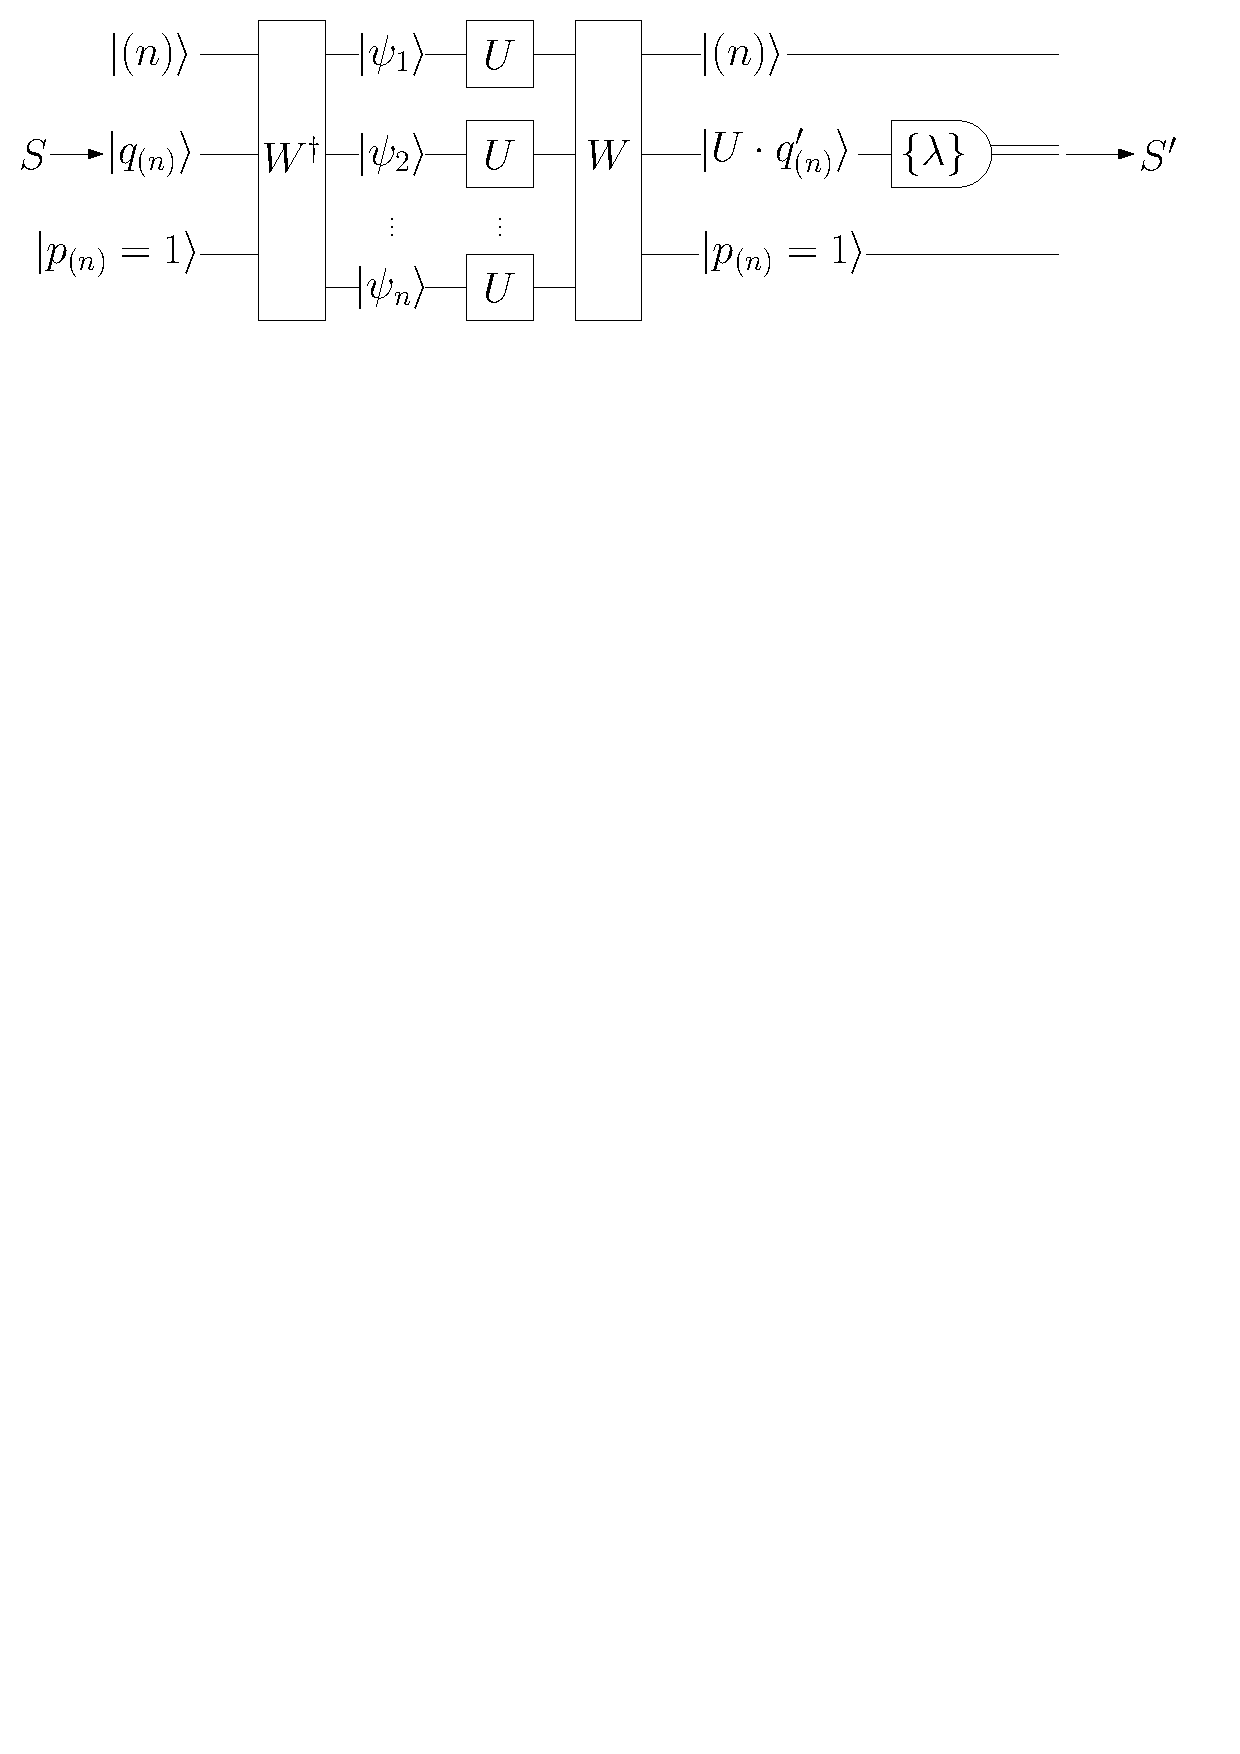
\includegraphics[width=\linewidth]{noisy_circuit/noiseless_circuit_irrep}
\caption{
A quantum circuit for Algorithm \ref{alg:bs}. 
Note that the measurement of the $q$-register returns a string that we associate to a GZ basis state.}
\label{fig:bs}
\end{figure}

We can demonstrate correctness by showing that this distribution does indeed match the one we have for sampling from indistinguishable bosons. 
We start with the input occupation $S$. 
After mapping this to a unitary irrep state $|q_{(n)}\rangle$ and applying $W^\dagger$, we end up with the symmetrized state
\begin{equation}\label{eq:IdealState}
W^\dagger\ket{\lambda=(n)}|q_{(n)}\rangle\ket{p_{(n)}=1}
 = \frac{1}{\sqrt{n! \prod_{i=1}^m S_i!}}\sum_{\sigma \in  \textrm{S}_n}\sigma|s\rangle ,
\end{equation}
where $|s\rangle$ can be chosen to be any computational basis state with occupation $S$, that is, with $S_i$ of the qudits in state $i$.
Arguing similarly for the output $S'$, we see that the probability of the algorithm outputting $q_{(n)}'$ given inputs $U$ and $S$ is
\begin{align}
\textrm{Pr}[q_{(n)}']
&= \vert \langle (n), q_{(n)}', 1\vert W U^{\otimes n} W^\dag |(n), q_{(n)}, 1\rangle \vert^2 \\
&= \left|\frac{1}{n!\sqrt{\prod_{i=1}^m S'_i! S_i!}}\sum_{\sigma, \sigma'\in \textrm{S}_n}\langle s'|{\sigma}'^\dag{U}^{\otimes n}{\sigma}|s\rangle\right|^2\\
&= \frac{1}{\prod_{i=1}^m S'_i! S_i!}\left|\frac{1}{n!}\sum_{\sigma, \sigma'\in \textrm{S}_n}\bigotimes_{k=1}^n \langle s'_{\sigma'^{-1}(k)}|{U}|s_{\sigma^{-1}(k)}\rangle\right|^2\\
&= \frac{1}{\prod_{i=1}^m S'_i! S_i!}\left|\frac{1}{n!}\sum_{\sigma, \sigma'\in \textrm{S}_n}\prod_{k=1}^n U_{s'_{k},s_{\sigma^{-1}(\sigma'(k))}}\right|^2\\
&= \frac{1}{\prod_{i=1}^m S'_i! S_i!}\left|\sum_{\tau \in \textrm{S}_n}\prod_{k=1}^n U_{s'_{k},s_{\tau(k)}}\right|^2\\
&= \frac{|\per(U_{S',S})|^2}{\prod_{i=1}^m S'_i! S_i!}.
\end{align}
Thus the output probability distribution matches the one given in Eq.~(\ref{eqn:bs-distribution}).
We also see that Schur-Weyl duality implies
\begin{equation}
U^{(n)}_{q_{(n)}, q_{(n)}'} = \frac{\per(U_{S',S})}{\sqrt{\prod_{i=1}^m S'_i! S_i!}}.
\label{eqn:symmetric_action}
\end{equation}
That is, the totally symmetric representation of the unitary group can be constructed from permanents of $U_{S',S}$ matrices~\cite{bhatia1997}.

As for the complexity of this circuit, the mapping from bosons to $q_{(n)}$ states and back can be done in polynomial time and space in terms of $n$~\cite{rowe1999}, Schur-Weyl duality takes polynomial time and space in terms of $d$, $n$ \& $\log(\delta^{-1})$ and the Solovay-Kitaev theorem allows $U$ to be implemented in polynomial time and space. 
From this and the earlier points discussed in this section, we find that Theorem \ref{thm:bs} holds.
\begin{theorem}
Algorithm \ref{alg:bs} performs ideal bosonic sampling with approximation $\delta+\epsilon$ in polynomial time and space in terms of $m$, $n$, $\log(\delta^{-1})$ and $\log(\epsilon^{-1})$.
\label{thm:bs}
\end{theorem}

We observe that this circuit could be simplified in several ways.
Firstly, the entire Schur transform is not required because in the ideal case the problem is confined to the symmetric irrep only.
As we will see, in the non-ideal (distinguishable) case other irreps can occur.

Another simplification that we'll use in the next section is the following observation.
If rather than applying step 5 onwards in Algorithm \ref{alg:bs} we simply measure the registers in the computational basis and return the result rewritten as an occupation, we also end up with a distribution given by the permanents. 
The probability of measuring a particular computational basis state $|s'\rangle \in (\mathbb{C}^m)^{\otimes n}$ is
\begin{align}
\textrm{Pr}[s'] 
&= \frac{1}{n!\prod_{i=1}^m (S_i!)}\left|\langle s'|U^{\otimes n}\sum_{\sigma \in \textrm{S}_n}\sigma|s\rangle\right|^2\\
&= \frac{1}{n!\prod_{i=1}^m (S_i!)}\left|\sum_{\sigma \in \textrm{S}_N}\bigotimes_{k = 1}^n\langle s_k'|U|s_{\sigma^{-1}(k)}\rangle\right|^2\\
&= \frac{\left|\sum_{\sigma \in \textrm{S}_n}\prod_{k = 1}^n U_{s_k', s_{\sigma^{-1}(k)}}\right|^2}{n!\prod_{i=1}^m (S_i!)} \\
&= \frac{|\per(U_{S',S})|^2}{n!\prod_{j=1}^m (S_i!)}.
\end{align}
%This becomes the Boson Sampling distribution by mapping back to occupations. 
The probability of measuring an occupation $S'$ is equal to summing over the probabilities of all states $|s'\rangle$ of type $S'$, of which there are $n!/\prod_{i=1}^m (S_i'!)$.
We will consider both versions of this circuit in subsequent sections on sampling from distinguishable bosonic distributions.



\section{A quantum circuit for arbitrarily distinguishable bosonic sampling}
\label{sec:qc-noisy}

We now turn to the question of sampling from a distribution of partially distinguishable bosons, (again with no loss).
Distinguishability is modelled as correlation between the modes of the bosons' `System'  degrees of freedom, and new modes corresponding to `Label' degrees of freedom.
In order to accommodate the possibility of all $n$ bosons being completely distinguishable, the number of Label modes must be $n$ so that each boson can be correlated to a unique Label.
Thus there are now a total of $mn$ modes in the problem.
Physically we can think of the System degree of freedom as the spatial modes available to the bosons, and the Label as, say, temporal modes -- however the model is completely general. 

On the aggregate Hilbert space we have the same setup as the ideal case, but now by tracing out the Label register we see that distinguishability can lead to decoherence of the System qudits.
We assume that an interferometer implementing an $m \times m$ unitary matrix acts only on the $m$ System modes, while the Label remains unchanged. 
In this model, as well as receiving a unitary matrix $U$ as input, we also receive an $m \times n$ occupation $T$ which describes how many bosons are in System mode $i$ and Label mode $j$. 
This can be described in terms of creation operators as
\begin{equation}
|T\rangle = \prod_{i=1}^m \prod_{j = 1}^n \frac{(a_{i,j}^\dagger)^{T_{i,j}}}{\sqrt{T_{i,j}!}}|0\rangle.
\end{equation}
Since the Labels are assumed to be unaffected by the interferometer, the creation operators evolve as $a_{i, j}^\dagger \rightarrow \sum_{k = 1}^m U_{i,k}a_{k, j}^\dagger$.

Our technique for handling distinguishable bosons is similar to the ideal case where we consider the symmetric irrep $\{(n)\}$ of the Unitary group. 
However, the introduction of the Label degree of freedom means that we no longer map onto the $\{(n)\}$ irrep of $\mathrm{U}(m)$. 
%Instead, we use a technique similar to the one employed by Adamson et al.~\cite{adamson2008} and later by Turner~\cite{turner2016}. 
Instead we must map onto the $\{(n)\}$ irrep of the aggregate unitary group $\mathrm{U}(mn)$, since it is now the total state of $m$ System modes and $n$ Label modes that must be symmetrised.

When we apply $W^\dagger$ to the input, we find the same Young symmetrizer as before, but now output a state $|\Psi\rangle \in (\mathbb{C}^m\otimes\mathbb{C}^n)^{\otimes n}$. 
We can think of this as the ideal case but now with each qudit being $mn$ dimensional.
Furthermore each System-Label qudit can be viewed as bipartite, with an $m$-dimensional qudit describing the System degree of freedom and another $n$-dimensional qudit describing the Label. 
We can therefore split the $n$ System-Label qudits into two registers, with the interferometer action and boson detection taking place on only the System register, while the Label register `eavesdrops'.
A complete description of the circuit is given in Algorithm \ref{alg:noisy-bs}, with a circuit diagram given in Figure \ref{fig:noisy-bs}.
\begin{algorithm}
\SetKwInOut{Input}{input}\SetKwInOut{Output}{output}
\Input{A matrix $U \in \textrm{U}(m)$ and \\ an $n$-boson $mn$-mode occupation $T$.}
\Output{An $n$-boson $m$-mode occupation $S'$.}
\BlankLine
Map $T$ to $q$-register basis index $q_{(n)}$ (for U$(mn)$)\;
Prepare input state $|\lambda=(n)\rangle|q_{(n)}\rangle|p_{(n)}=1\rangle$\;
Apply $W^\dagger$, producing a state $|\Psi\rangle \in (\mathbb{C}^{m \times n})^{\otimes n}$\;
Rearrange into two (possibly entangled) quantum registers $|\Psi_{\textrm{Sys}}\rangle = |\psi_{\textrm{Sys}, 1}\rangle\dots|\psi_{\textrm{Sys}, n}\rangle \in (\mathbb{C}^m)^{\otimes n}$ and $|\Psi_{\textrm{Lab}}\rangle = |\psi_{\textrm{Lab}, 1}\rangle\dots|\psi_{\textrm{Lab}, n}\rangle \in (\mathbb{C}^{n})^{\otimes n}$\;
%\tcc{(Note that these registers might be entangled)}
Synthesize $U$ via Solovay-Kitaev\;
Execute $U$ on the $|\Psi_{\textrm{Sys}}\rangle$ qudits in parallel, implementing  $U^{\otimes n} \otimes \Id_\mathrm{Lab}$\;
Measure the System in the computational basis to obtain a sample $s'$\;
Map $s'$ to an occupation $S'$ ($S'_i = \#$ of qudits in state $1\leq i\leq m$)\;
\Return $S'$
\caption{A quantum circuit for sampling from (essentially) the same distribution at that produced by distinguishable bosons in a linear interferometer.
In order to sample from exactly the same distribution, instead of step 7 one could transform back to the Schur basis by applying $W$ on the System and sample the $q$-register, or one could perform some post-processing as discussed at the end of the previous section.}
\label{alg:noisy-bs}
\end{algorithm}

\begin{figure}
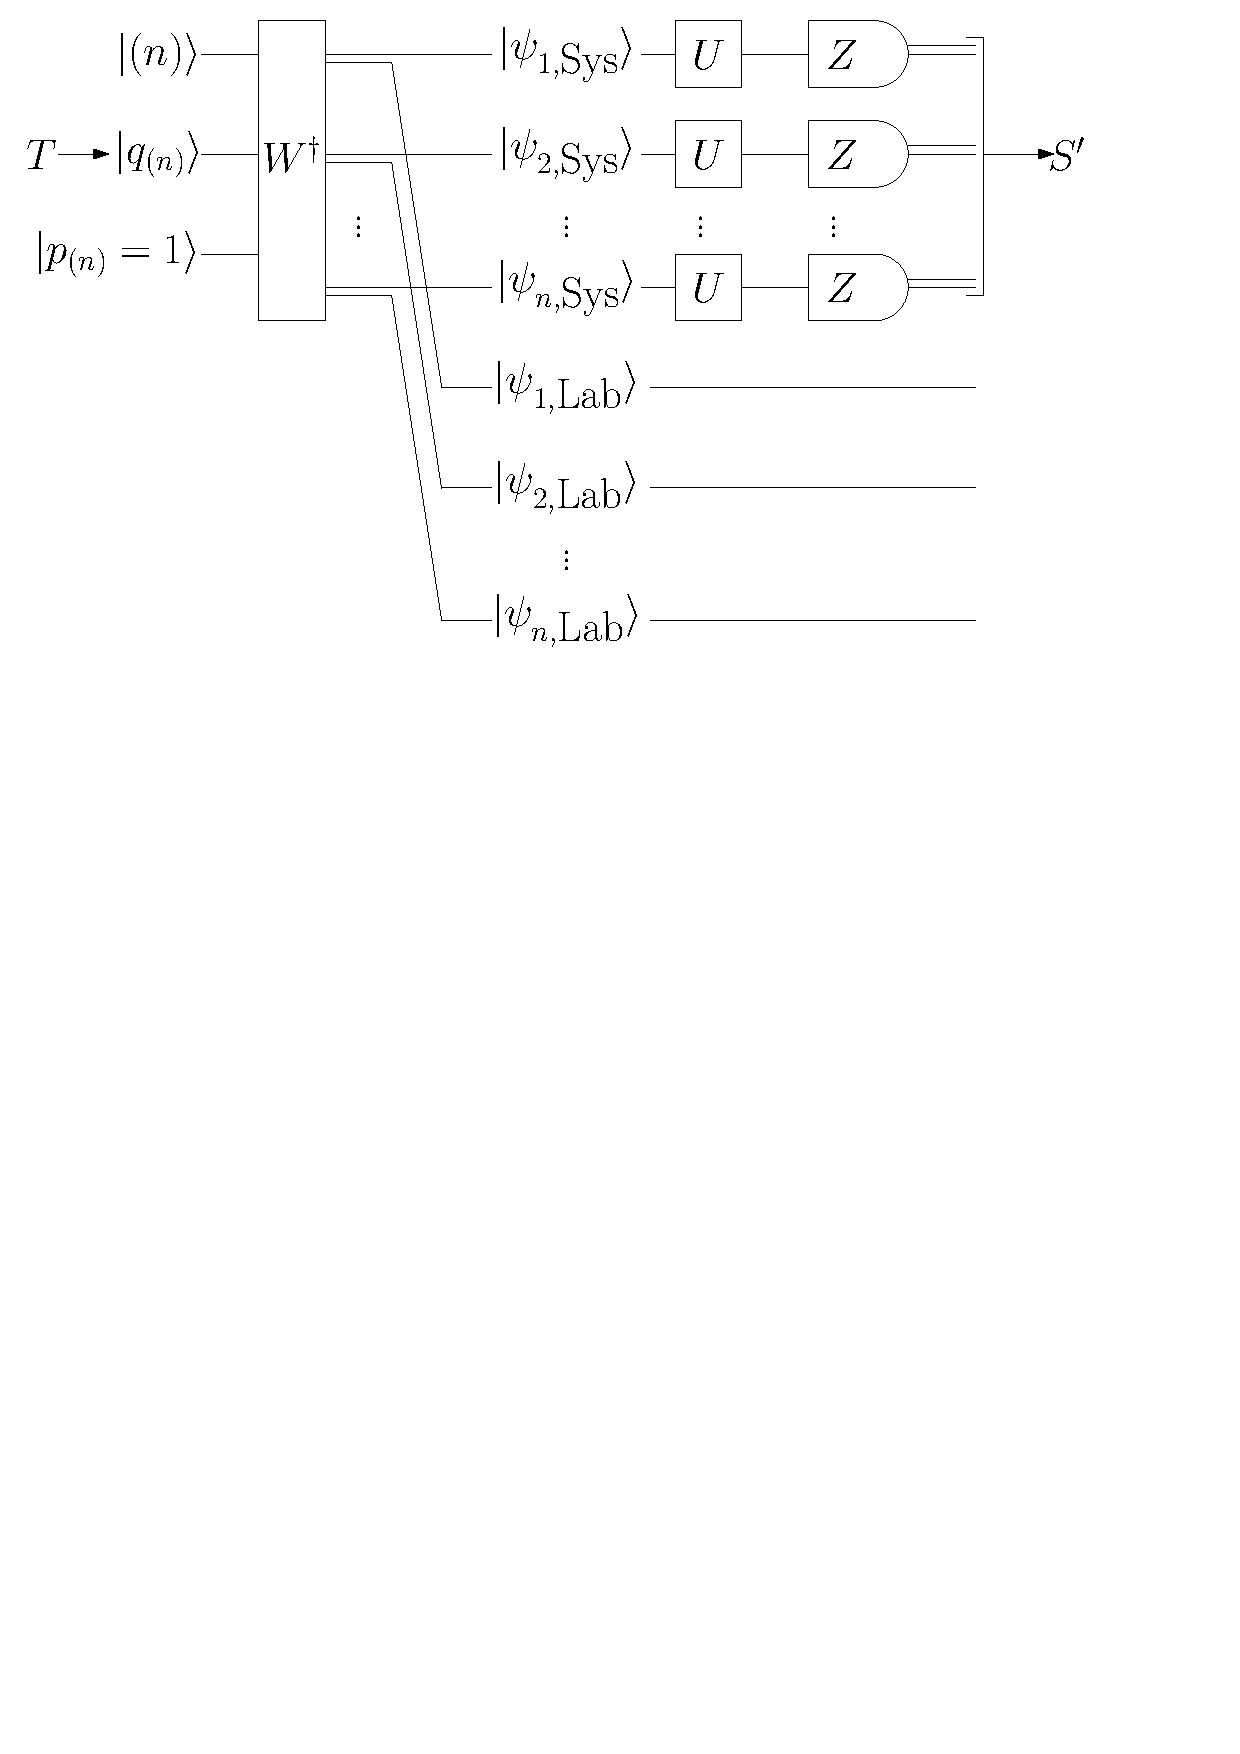
\includegraphics[width=\linewidth]{noisy_circuit/noisy_circuit_fig}
\caption{The quantum circuit described in Algorithm \ref{alg:noisy-bs}. 
For simplicity we forego the second Schur transform as discussed in the previous section and measure in the computational ($Z$) basis. 
Note that we only sample from the System qudits, effectively tracing out the Label qudits.}
\label{fig:noisy-bs}
\end{figure}

To see that this distribution matches that of partially distinguishable bosons, we will compare with the results of Tichy~\cite{tichy2015}.
There, each boson is assigned an ``internal'' state $|\Phi_i\rangle$, where $i=1, \cdots, m$.
Thus, in our terminology, every boson in System mode $i$ has a Label state given by $\Phi_i$.
The probability distribution given there for sampling from partially distinguishable bosons is (in our notation)
\begin{equation}\label{eq:TichyDist}
\textrm{Pr}[S'] =  \frac{1}{\prod_{i=1}^m S_i! S'_i!} \sum_{\tau, \tau' \in \textrm{S}_n} \prod_{k=1}^n U_{s'_k,s_{\tau(k)}} U^\ast_{s'_k,s_{{\tau'}(k)}} \mathcal{S}_{{\tau'(k)},{\tau(k)}},
\end{equation}
where $\mathcal{S}_{k,l} = \langle \Phi_{s_k}|\Phi_{s_l}\rangle$ is a Hermitian positive-definite $n \times n$ distinguishability matrix, $s_k$ gives the mode occupied by particle $k$, and we've included a factor to account for the possibility of multiple bosons in the same output mode.
In order to connect our model with this model of distinguishability, one simply needs to take superpositions of $mn$-mode input occupations $T$ in such a way as to realise the Label states $\Phi_i$.
This is always possible since the space of internal states, span$\{\Phi_i\}_{i=1}^m$, can always be embedded in the Label space $(\mathbb{C}^n)^{\otimes n}$.
For example, consider two bosons in two System modes where one boson is in System mode 1 and has internal state $|1\rangle$ (corresponding to Label mode 1), and the other boson is in System mode 2 and has internal state $|\Phi_2\rangle=\alpha|1\rangle+\beta|2\rangle$.
This is represented as the following superposition of System-Label occupations (recall rows of $T$ correspond to the System and columns to the Label):
\begin{align}
\alpha \Ket{\begin{matrix} 1&0\\1&0 \end{matrix}} + \beta \Ket{\begin{matrix} 1&0\\0&1 \end{matrix}} .
\end{align}
Given a distinguishability matrix $\mathcal{S}_{k,l}$, in this way we can prepare a corresponding superposition of occupations $T$ at step 2 of the algorithm.
(We can in fact consider more general partially distinguishable situations of bosons with different Label states in the same System mode.)

After step 3 of the algorithm, the state can be written as
\begin{align}
|\Psi\rangle_{\textrm{Sys,Lab}}
 &= \frac{1}{\sqrt{n!\prod_{i=1}^m S_i!}}\sum_{\sigma\in\textrm{S}_n}\sigma|s\rangle\sigma\bigotimes_{k=1}^n|\Phi_{s_k}\rangle\\
 &= \frac{1}{\sqrt{n!\prod_{i=1}^m S_i!}}\sum_{\sigma\in\textrm{S}_n}\sigma|s\rangle\bigotimes_{k=1}^n|\Phi_{s_{\sigma^{-1}(k)}}\rangle\\
\end{align}
where $|s\rangle=\bigotimes_{k=1}^n|s_k\rangle$ and $\bigotimes_{k=1}^n|\Phi_{s_k}\rangle$ are quantum registers describing the System and Label. 
Tracing out the Label register yields the reduced density matrix
\begin{align}
\rho_{\textrm{Sys}}
 &= \textrm{Tr}_{\textrm{Lab}}[|\Psi\rangle_{\textrm{Sys,Lab}}\langle\Psi|]\\
 &= \frac{1}{n!\prod_{i=1}^m S_i!}\sum_{\sigma,\sigma'\in\textrm{S}_n}\sigma|s\rangle\langle s|\sigma'^\dagger \prod_{k=1}^n \langle\Phi_{s_{\sigma'^{-1}(k)}}|\Phi_{s_{\sigma^{-1}(k)}}\rangle\\
 &=\frac{1}{n!\prod_{i=1}^m S_i!}\sum_{\sigma,\sigma'\in\textrm{S}_n}\sigma|s\rangle\langle s|\sigma'^\dagger \prod_{k=1}^n \mathcal{S}_{\sigma'^{-1}(k),\sigma^{-1}(k)}.
\end{align}
When we apply the action of the interferometer $U$ on the $m$-dimensional System qudits, the probability of measuring a state $|s'\rangle$ after step 7 is
\begin{align}
\textrm{Pr}[|s'\rangle] 
 &= \textrm{Tr}[|s'\rangle\langle s'|U^{\otimes n}\rho_{\textrm{Sys}}(U^\dagger)^{\otimes n}]\\
 &= \frac{\sum_{\sigma, \sigma' \in \textrm{S}_n}\langle s'|U^{\otimes n}\sigma|s\rangle\langle s|\sigma'^\dagger(U^\dagger)^{\otimes n}|s'\rangle \prod_{k=1}^n\mathcal{S}_{\sigma'^{-1}(k),\sigma^{-1}(k)}}{n!\prod_{i=1}^m S_i!}\\
 &= \frac{\sum_{\sigma, \sigma' \in \textrm{S}_n} \prod_{k=1}^n \langle s'_k|U|s_{\sigma^{-1}(k)}\rangle\langle s_{\sigma'^{-1}(k)}|U^\dagger|s'_k\rangle\mathcal{S}_{\sigma'^{-1}(k),\sigma^{-1}(k)}}{n!\prod_{i=1}^m S_i!}\\
 &= \frac{\sum_{\tau, \tau' \in \textrm{S}_n} \prod_{k=1}^n U_{s'_k,s_{\tau(k)}} U^*_{s'_k,s_{\tau'(k)}} \mathcal{S}_{\tau'(k),\tau(k)}}{n!\prod_{i=1}^m S_i!}.
\end{align}
Up to a factor, this is the desired probability distribution of Eq.(\ref{eq:TichyDist}).
As discussed at the end of the last section, this factor could be handled either by applying a second Schur transform on the System and sampling the $q$-register, or by classical post processing.

Counting resources goes much the same as it did in the ideal case, though now we have $mn$-dimensional qudits that are made up of pairs of $m$- and $n$-dimensional qudits.
Separating these System and Label registers in step 3 can be done with polynomial resources, as can the unitary transformation on the input $q$-register that prepares the input state of arbitrary distinguishability.
From this and the points above, we find that Theorem \ref{thm:noisy-bs} holds.
\begin{theorem}
Algorithm \ref{alg:noisy-bs} samples from the distinguishable bosonic distribution with approximation $\delta+\epsilon$ when the distinguishability of the input bosons is known. 
The circuit runs in polynomial time and space in terms of $m, n, \log(\delta^{-1})$ and $\log(\epsilon^{-1})$.
\label{thm:noisy-bs}
\end{theorem}


\subsection{Complete (in)distinguishability}

The two extreme cases of completely indistinguishability and complete distinguishability are of interest.
For completely indistinguishable bosons, the Label for each is the same (call it $\ket{1}$), and after the (inverse) Schur transform step we have
\begin{equation}
\frac{1}{\sqrt{n!\prod_{i=1}^m S_{i}!}}\sum_{\sigma\in \textrm{S}_n}\sigma|s\rangle|1\rangle^{\otimes n},
\end{equation}
It is clear that the Label register is separable from the System register, and tracing out the Label yields the same situation as the ideal case in Eq.(\ref{eq:IdealState}), as it should.

In the completely distinguishable case, each boson has a different unique Label, correlated to a unique System mode (note $m\geq n$ in this case).
This implies that the occupation $T$ has a single 1 in each of $n$ rows and columns, and zeros elsewhere.
The (inverse) Schur transformed state has System and Label registers $s$ and $l$ that are completely correlated sequences of length $n$ with no repetitions; if we choose to order the bases $123\cdots n$ then we have the state

\begin{align}\label{eq:ComDis}
\frac{1}{\sqrt{n!}} \sum_{\sigma \in \textrm{S}_n}\sigma|s\rangle\sigma|l\rangle
&=\frac{1}{\sqrt{n!}} \sum_{\sigma \in \textrm{S}_n}|\sigma^{-1}(1) \sigma^{-1}(2) \cdots \sigma^{-1}(n)\rangle |\sigma^{-1}(1) \sigma^{-1}(2) \cdots \sigma^{-1}(n)\rangle .
\end{align}
We see that this is maximally entangled on the ``coincident'' subspace of states with a single boson in each mode.
Tracing out the Label yields the reduced System state
\begin{align}
\rho_\mathrm{Sys}
 &= \frac{1}{n!} \sum_{\sigma, \sigma' \in \textrm{S}_n} \sigma|s\rangle\langle s|\sigma'^\dagger \, \langle l|\sigma'^\dagger \sigma|l\rangle \\
 &= \frac{1}{n!} \sum_{\sigma \in \textrm{S}_n} \sigma|s\rangle\langle s|\sigma^\dagger ,
\end{align}
which follows because the Label overlap is only nonzero if $\sigma'^\dag \sigma = \Id \Rightarrow \sigma'=\sigma$ due to the fact that $l$ has no repetitions.
After the action of $U$, the probability of measuring $|s'\rangle \in (\mathbb{C}^m)^{\otimes n}$ is
\begin{align}
\textrm{Pr}[|s'\rangle]
 &= \textrm{Tr}[|s'\rangle\langle s'|U^{\otimes n}\rho_\mathrm{Sys} U^{\dagger\otimes n}]\\
 &= \frac{1}{n!} \langle s'|U^{\otimes n}\left(\sum_{\sigma \in  \textrm{S}_n}\sigma|s\rangle\langle s|\sigma^\dagger\right)U^{\dagger\otimes n}|s'\rangle\\
% &= \frac{1}{n!} \sum_{\sigma \in  \textrm{S}_n} \prod_{k=1}^n\langle s_k'|U|s_{\sigma^{-1}(k)}\rangle\langle s_{\sigma^{-1}(k)}|U^\dagger|s_k'\rangle\\
 &= \frac{1}{n!} \sum_{\sigma \in  \textrm{S}_n} \prod_{k=1}^n |U_{s'_k,s_{\sigma^{-1}(k)}}|^2\\
 &= \frac{\textrm{per}(|U_{S',S}|^2)}{n!} ,
\end{align}
where we've defined $|U_{S',S}|^2$ as the elementwise square of the absolute value.
We can find the probability of returning occupation $S'$ by summing up the probabilities of all $n!/\prod_{i=1}^{m}(S'_i!)$ states of type $s'$, giving
\begin{equation}\label{eq:DistPer}
\textrm{Pr}[S'] = \frac{\textrm{per}(|U_{S',S}|^2)}{\prod_{i=1}^m S'_i!},
\end{equation}
which agrees with the (classical) probability distribution for sampling with distinguishable bosons~\cite{aaronson2014}.

%Note that we could have considered a distinguishable input where each boson has a unique Label, but with multiple occupancy of System modes.
%In that case the analysis would show the output distribution to be the same as above up to a factor of $\prod_i S_i!$ in the denominator. \FIXME{I'm not entirely sure this paragraph is right. The $S_i!$ terms are essentially just normalisation of the initial state, but there are only $n!$ terms in the fully distinguishable case anyway as it is zeros everywhere except the diagonal. Very minor thing anyway.}
%{\blue I think this subsection is pretty clear, the reader should be able to produce the 2 photon calculations themself so probably not necessary to include the appendix.}



\section{Unitary-unitary duality}
\label{sec:uu-duality}

The preceding shows how the Schur transform gives a map between second quantised occupation states and first quantised single particle states via symmetrisation.
The complication added by distinguishability is that each single particle becomes bipartite, with a System and Label degree of freedom.
As shown above, distinguishability arises as correlations between the System and Label registers of the circuit in Fig.~\ref{fig:noisy-bs}.
It turns out that independently transforming the System and Label registers back into the Schur basis can give a Schmidt decomposition for these correlated states (see Fig.~\ref{fig:noisy-bs-rep}).
This can be seen as a consequence of the following duality~\cite{goodman2009, rowe2012}.
\begin{theorem}[Unitary-unitary duality]\label{thm:unitary-unitary}
The totally symmetric irrep of $\mr{U}(md)$ can be decomposed into irreps of $\mr{U}(m) \times \mr{U}(d)$ as
\begin{align}\label{eq:uudecomp}
(\mathbb{C}^{m} \otimes \mathbb{C}^{d})^{(n)} \cong \bigoplus_{\lambda\vdash n} \mathbb{C}^{\{\lambda\}_m} \otimes \mathbb{C}^{\{\lambda\}_d} ,
\end{align}
where $\{\lambda\}_m$ indicates an irrep $\lambda$ of $\mr{U}(m)$, similarly for $\{\lambda\}_d$, and $\lambda$ runs over all partitions of $n$ consistent with both $m$ and $d$.
\end{theorem}
This can be proven by Schur decomposing the System and Label registers, each of which, by Schur-Weyl duality, will have good permutation symmetry quantum numbers.
The question is then which linear combinations of tensor products of such states are totally symmetric, and the answer turns out to be only states of the form (suppressing normalisation)~\cite{hamermesh1962}
\begin{align}\label{eq:symSL}
\ket{\lambda, q_\lambda, {q'}_\lambda}_\mr{SysLab} &=  \sum_{p_\lambda} \ket{\lambda, q_\lambda, p_\lambda}_\mr{Sys} \ket{\lambda, {q'}_\lambda, p_\lambda}_\mr{Lab} .
\end{align}
Thus a basis for the totally symmetric irrep of the System-Label Hilbert space consists of states of this form, leading to the decomposition in Eq.(\ref{eq:uudecomp}) and to a Schmidt decomposition of totally symmetric (second quantised) System-Label states.

Because the Schur transformations on each register are local to the System and Label, entanglement across this bipartition is unchanged.
For example, the completely distinguishable state that from Eq.(\ref{eq:ComDis}) is seen to have Schmidt rank $n!$ in the computational basis, and therefore must be of the form
\begin{equation}
\frac{1}{\sqrt{n!}} \sum_{\lambda \vdash n} \sum_{q_\lambda^\mr{coin}} \sum_{p_\lambda} |\lambda,q_\lambda,p_\lambda\rangle_{\textrm{Sys}}|\lambda,q_\lambda,p_\lambda\rangle_{\textrm{Lab}},
\end{equation}
where the sum over $q_\lambda^\mr{coin}$ is taken over the coincident subspace, that is, the irrep basis states with pattern weight (or type) $(11\cdots 1)$.
That the dimensions of these spaces are the same can be shown combinatorially and follows from the theorem.
This shows that although in the ideal case only the symmetric subspace is in play and therefore the full Schur transform is overkill, for the distinguishable case all irreps $\lambda$ can play a role.

\begin{figure}
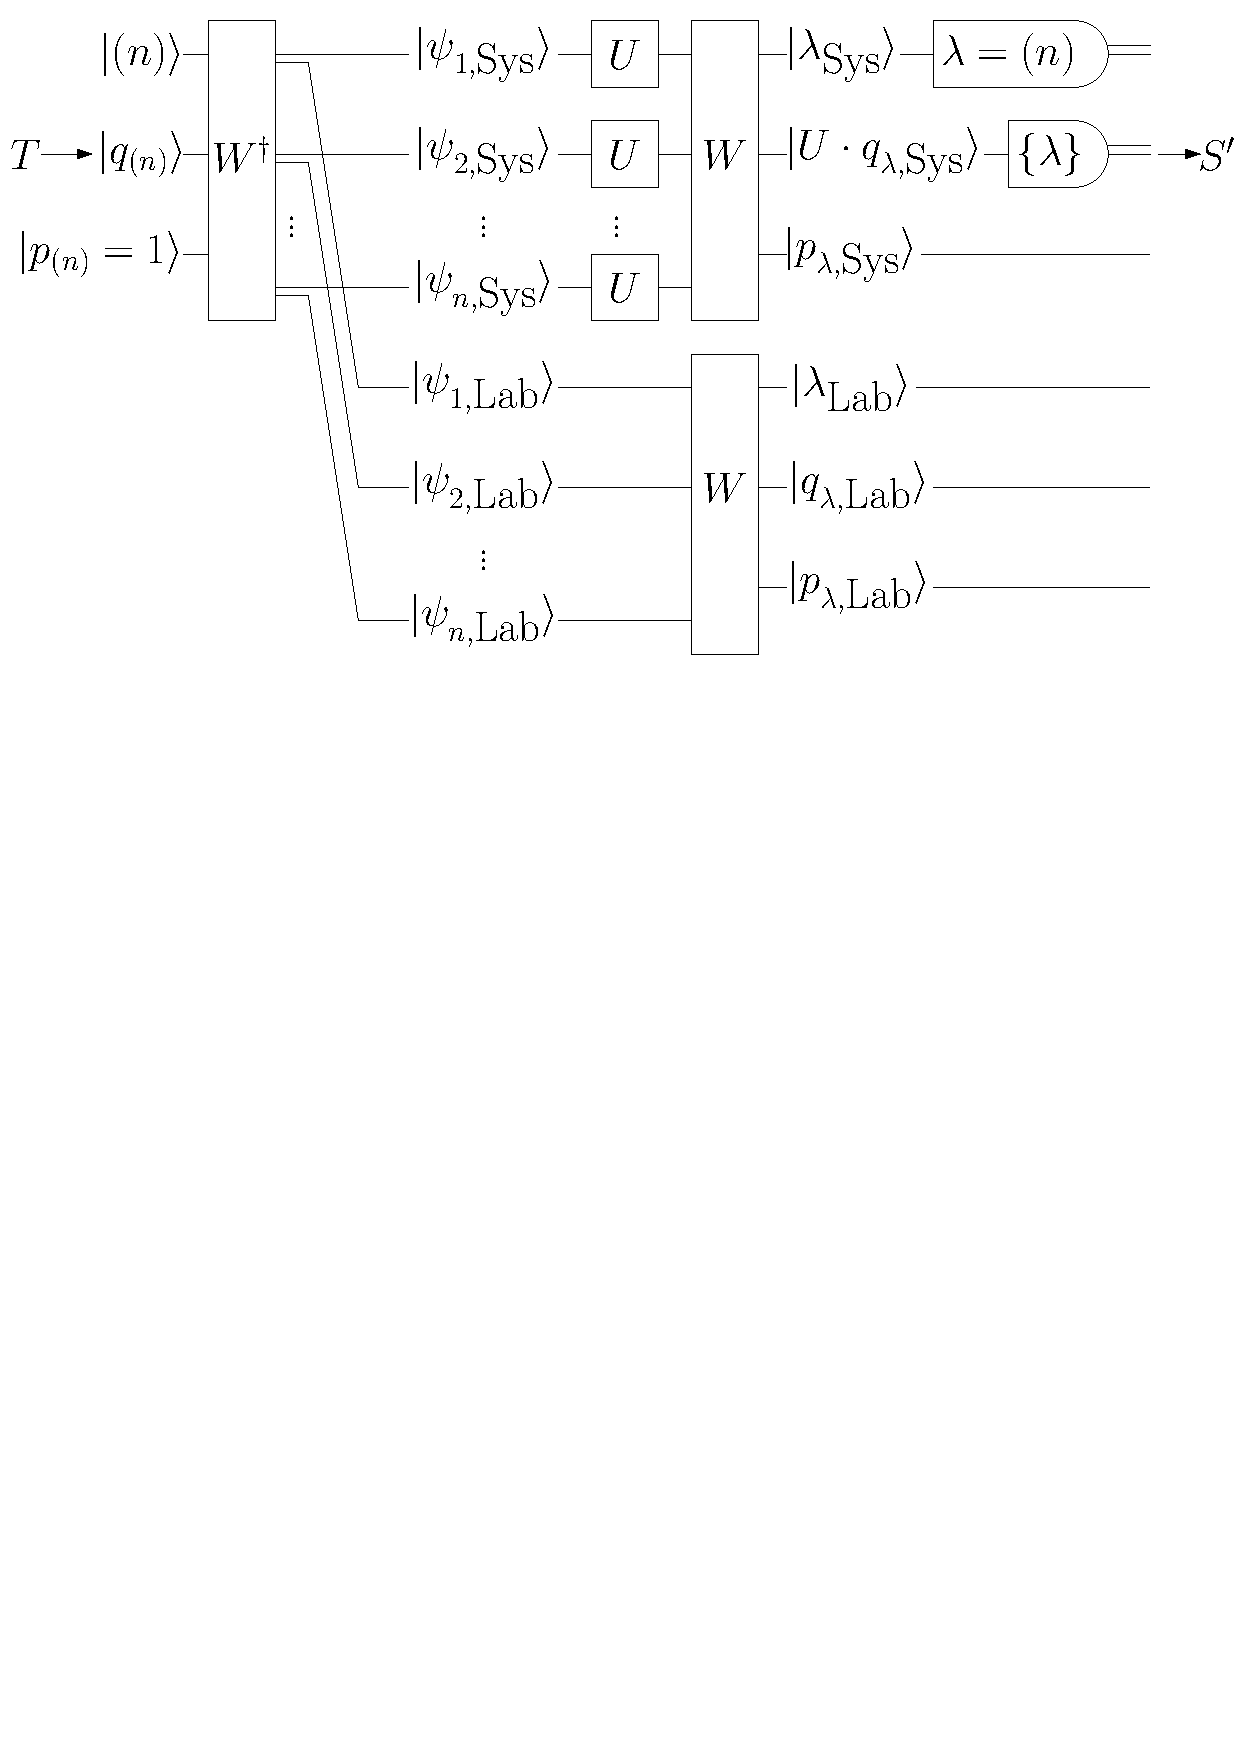
\includegraphics[width=\linewidth]{noisy_circuit/post_circuit}
\caption{Circuit diagram illustrating how postselection can be used to `filter out' distinguishability.
Note that the postselection measurement of the System $\lambda$-register is in the irrep basis, while that of the System $q$-register is in the GZ basis.
The second Schur transform on the Label register is not necessary, but illustrates the unitary-unitary duality.}
\label{fig:noisy-bs-rep}
\end{figure}


\subsection{Postselection of ideal bosonic sampling}
\label{sec:post-bs}

Although unitary-unitary duality can be demonstrated in this model by implementing local Schur transforms before measuring, in both the ideal and distinguishable case circuits considered previously, it was argued that this was not necessary; it was enough to measure in the computational basis after the unitary transformation was implemented and post-process.
An interesting observation is that given a distinguishable input, by performing the second Schur transform on the System it becomes possible to use postselection to sample from the indistinguishable distribution.
Of course, this comes at the cost of throwing away a lot of bad samples.

To achieve this postselective filtering, we need to ensure that we only sample the System from the fully symmetric irrep of $\textrm{U}(m)$. 
This is done by measuring the irrep register $|\lambda\rangle_{\textrm{Sys}}$ and waiting for the outcome $\lambda_{\textrm{Sys}}=(n)$. 
After postselection, the amplitudes of the System $q$-register $|U\cdot q_{(n)}\rangle$ are given by Eq.~\ref{eqn:symmetric_action}, which give the same probability distribution as sampling indistinguishable bosons. 
Following the arguments above, the circuit remains efficient since the added Schur transform can be implemented efficiently. 

More generally, such a postselected quantum circuit could sample from any irrep $\lambda$ of $\textrm{U}(m)$. 
All we need to achieve this is to ensure that the input state has support in the irrep we wish to sample from, and postselect on being in that irrep.
A dimension counting argument shows that the completely distinguishable input discussed above has support in all irreps~\cite{stanisic2018}, and so could be used for this purpose.
%We will discuss the complexity of such sampling in Sec.~\ref{sec:conclusion}.



\section{Sampling with loss}
\label{sec:loss}

Another serious practical difficulty with linear optics is the loss of photons through unwanted scattering processes. 
In this section, we discuss how the loss model developed by Aaronson and Brod~\cite{aaronson2015} can be simulated. 
In their model, $n+k$ bosons are generated as occupation $S^0$, $k$ of which are lost before they reach the interferometer. 
As we don't know which bosons were lost, Aaronson and Brod take the average over the set of all $n$-boson occupations which are consistent with $S^0$, denoted $\bar{\Lambda}_{m,S^0,n}$.
The result can be shown by tracing out any choice of $k$ qudits in the ideal case, as shown in Fig.~\ref{fig:lost-bs}. 

\begin{figure}
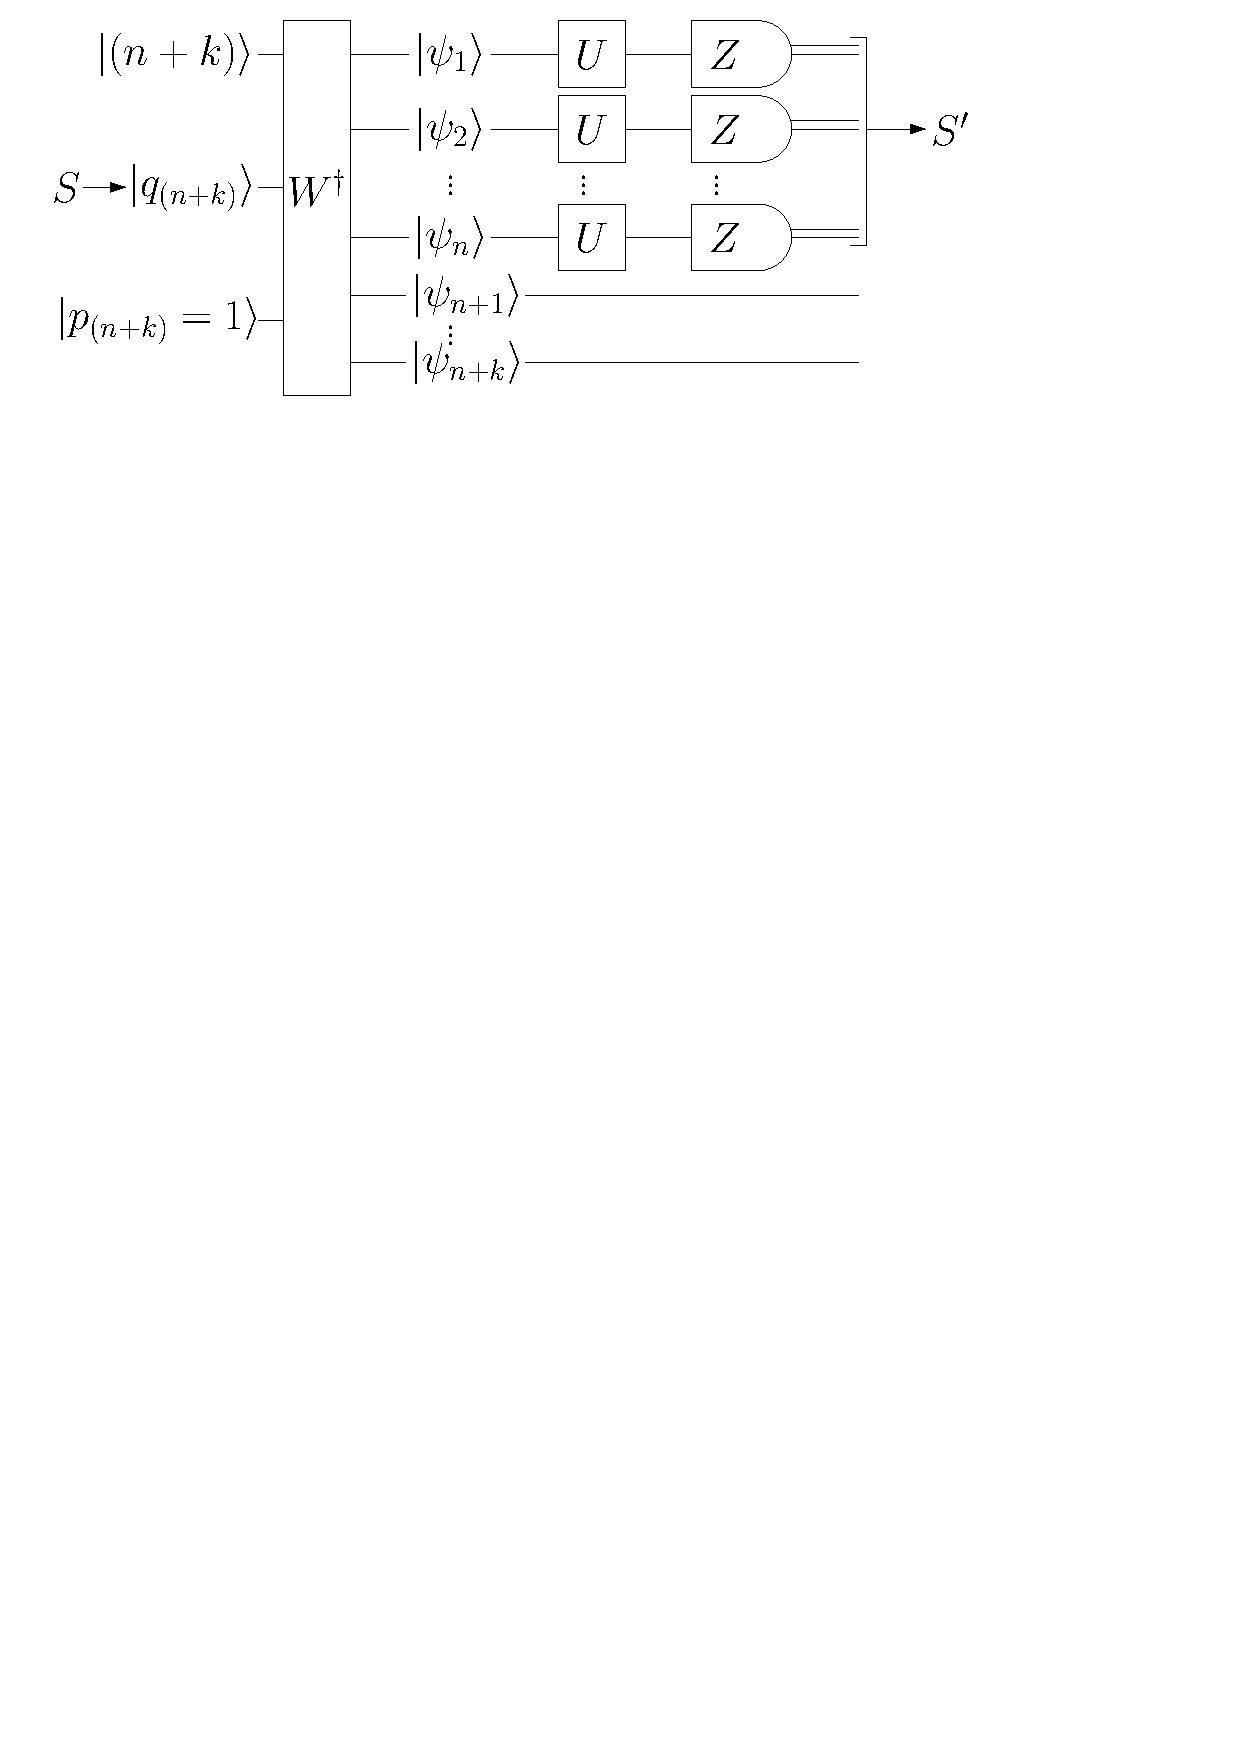
\includegraphics[width=\linewidth]{noisy_circuit/lost_circuit}
\caption{Circuit for sampling when $k$ bosons are lost. 
Here, we ignore $k$ qudits of the System register, tracing them out with the Label register. 
As with Fig.~\ref{fig:noisy-bs}, measurements are in the computational basis.}
\label{fig:lost-bs}
\end{figure}

\begin{theorem}
Let $|\psi\rangle$ be the state after step 2 of Algorithm \ref{alg:bs} with $(n+k)$-boson input state $S^0$, and $\bar{\Lambda}_{m,S^0,n}$ be the set of all $n$-boson occupations which are consistent with $S^0$.
If $k$ qudits of $|\psi\rangle$ are traced out before continuing with the algorithm, the final probability distribution of output occupations $S'$, denoted $\mathcal{D}_U$, is
\begin{equation}
\mr{Pr}_{\mathcal{D}_U}[S'] = \frac{1}{\binom{n+k}{k}}\sum_{S \in \bar{\Lambda}_{m,S^0,n}} |\mr{per}(U_{S',S})|^2 \prod_{i=1}^m \frac{\binom{S_i^0}{S_i}}{S'_i! S_i!} .
\end{equation}
\end{theorem}

\begin{proof}
The state $|\psi\rangle$ can be written as the density matrix
\begin{equation}
\rho = |\psi\rangle\langle\psi| = \frac{1}{(n+k)!\prod_{i=1}^m S^0_i!} \sum_{\sigma\in\textrm{S}_{n+k}}\sigma|s^0\rangle\sum_{\sigma'\in\textrm{S}_{n+k}}\langle s^0|\sigma'^\dagger,
\end{equation}
where $|s^0\rangle$ is any state consistent with the input state occupation $S^0$.
This state is symmetric, so the choice of which qudits to trace out is moot.
Choosing the last $k$ qudits, the reduced density matrix for the remaining $n$ particles is

\begin{align}
\rho_n
 &= \frac{1}{(n+k)!\prod_{i=1}^m S^0_i!}\sum_{\sigma,\sigma'\in\textrm{S}_{n+k}}\bigotimes_{l=1}^n|s^0_{\sigma^{-1}(l)}\rangle\langle s^0_{\sigma'^{-1}(l)}|\bigotimes_{l=n+1}^{n+k}\langle s^0_{\sigma'^{-1}(l)}|s^0_{\sigma^{-1}(l)}\rangle\label{eqn:losstrace}\\
 &=\frac{1}{(n+k)!\prod_{i=1}^m S^0_i!}\sum_{\substack{S \subseteq \{s^0_1,\dots,s^0_{n+k}\}\\\bar{S}=\{s^0_1,\dots,s^0_{n+k}\}\setminus{S}\\|S|=n}}\sum_{\sigma \in \textrm{S}_{n}}\sigma|s\rangle\sum_{\sigma' \in \textrm{S}_{n}}\langle s|\sigma'^\dagger\sum_{\tau,\tau'\in\textrm{S}_k}\langle \bar{s}|\tau'^\dagger\tau|\bar{s}\rangle\label{eqn:firstloss}\\
 &=\frac{1}{(n+k)!\prod_{i=1}^m S^0_i!}\sum_{\substack{S \in \Lambda_{m,S^0,n}\\\bar{S}=\{s^0_1,\dots,s^0_{n+k}\}\setminus{S}}}\prod_{i=1}^m\left(\frac{S^0_i!}{S_i!(S_i^0-S_i)!}\right)^2\sum_{\sigma \in \textrm{S}_{n}}\sigma|s\rangle\sum_{\sigma' \in \textrm{S}_{n}}\langle s|\sigma'^\dagger\sum_{\tau,\tau'\in\textrm{S}_k}\langle \bar{s}|\tau'^\dagger\tau|\bar{s}\rangle\label{eqn:secondloss}\\
 &=\frac{k!}{(n+k)!}\sum_{S \in \Lambda_{m,S^0,n}}\frac{\prod_{i=1}^m S^0_i!}{(\prod_{j=1}^m S_j!)^2\prod_{i=1}^m (S^0_i-S_i)!}\sum_{\sigma \in \textrm{S}_{n}}\sigma|s\rangle\sum_{\sigma' \in \textrm{S}_{n}}\langle s|\sigma'^\dagger\label{eqn:thirdloss}\\
 &=\frac{1}{\binom{n+k}{n}}\sum_{S \in \Lambda_{m,S^0,n}}\frac{\prod_{i=1}^m \binom{S_i^0}{S_i}}{n!\prod_{j=1}^m S_j!}\sum_{\sigma \in \textrm{S}_{n}}\sigma|s\rangle\sum_{\sigma' \in \textrm{S}_{n}}\langle s|\sigma'^\dagger , \label{eq:lastloss}
\end{align}
where now $|s\rangle$ (resp.\ $|\bar{s}\rangle$) is any state consistent with the occupation $S$ (resp.\ $\bar{S}$). 
In this calculation we first break the qudits into multisets of $S$ and $\bar{S}$ with respective sizes $n$ and $k$, and permute each multiset individually, which is done in Eq.(\ref{eqn:firstloss}). 
Note that $S \subseteq \{s^0_{1},\dots,s^0_{n+k}\}$ such that $|S|=n$ implies that $S\in\Lambda_{m,S^0,n}$ defined above, so we can sum over $\Lambda_{m,S^0,n}$. 
However, doing so will ignore duplicates of $S$ we had when considering multisets included in $\{s^0_1,\dots,s^0_{n+k}\}$, which need to be acconted for. 
The total number of duplicate terms is the number of permutations $\sigma,\sigma'\in\textrm{S}_{n+k}$ for which $|s^0\rangle$ is invariant, of which there are $(\prod_{i=1}^m S^0_i!)^2$. 
The permutations $\sigma,\sigma'\in\textrm{S}_n$ and $\tau,\tau'\in\textrm{S}_k$ mean that $(\prod_{i=1}^mS_i!(S_i^0-S_i)!)^2$ duplicates are already accounted for. 
Putting these two points together, we get the factor seen in Eq.(\ref{eqn:secondloss}). 
Finally in Eq.(\ref{eqn:thirdloss}), we take the inner product, noting that $\sum_{\tau,\tau'\in\textrm{S}_k}\langle \bar{s}|\tau'^\dagger\tau|\bar{s}\rangle = k!\prod_{i=1}^m(S_i^0-S_i)!$.

Applying the unitary transformation $U$ and measuring in the computational basis, we find that the calculation of the probability of measuring a state $|s'\rangle \in (\mathbb{C}^m)^{\otimes n}$ goes through much as in the previous sections.
Applying the same methods as before, we have
%\begin{widetext}
\begin{align}
&\textrm{Pr}[|s'\rangle]\\
&= \textrm{Tr}[|s'\rangle\langle s'|(U)^{\otimes n}\rho_n (U^\dagger)^{\otimes n}]\\
%&= \frac{1}{\binom{n+k}{n}}\sum_{S \in \bar{\Lambda}_{d,n+k,n}}\frac{\prod_{i=1}^d\binom{S_i^0}{S_i}}{n!\prod_{j=1}^dS_j!}\langle s'|U^{\otimes n}\left(\sum_{\sigma \in \textrm{S}_n}\sigma|s\rangle\right)\left(\sum_{\sigma' \in \textrm{S}_n}\langle s|\sigma'^\dagger\right)(U^\dagger)^{\otimes n}|s'\rangle\\
&= \frac{1}{\binom{n+k}{n}}\sum_{S \in \bar{\Lambda}_{m,n+k,n}} \frac{\prod_{i=1}^m \binom{S_i^0}{S_i}}{n!\prod_{j=1}^m S_j!} \left|\langle s'|U^{\otimes n}\left(\sum_{\sigma \in \textrm{S}_n}\sigma|s\rangle\right)\right|^2\\
%&= \frac{1}{\binom{n+k}{n}}\sum_{S \in \bar{\Lambda}_{d,n+k,n}}\frac{\prod_{i=1}^d\binom{S_i^0}{S_i}}{n!\prod_{j=1}^dS_j!}\left|\sum_{\sigma \in \textrm{S}_n}\bigotimes_{l=1}^n\langle s'_l|U|s_{\sigma^{-1}(s_l)}\rangle\right|^2\\
%&= \frac{1}{\binom{n+k}{n}}\sum_{S \in \bar{\Lambda}_{d,n+k,n}}\frac{\prod_{i=1}^d\binom{S_i^0}{S_i}\left|\sum_{\sigma \in \textrm{S}_n}\prod_{l=1}^nU_{s'_l,s_{\sigma^{-1}(l)}}\right|^2}{n!\prod_{j=1}^dS_j!}\\
&= \frac{1}{\binom{n+k}{n}}\sum_{S \in \bar{\Lambda}_{m,n+k,n}} |\mr{per}(U_{S',S})|^2 \prod_{i=1}^m \frac{\binom{S_i^0}{S_i}}{n!S_i!} .
\end{align}
%\end{widetext}
To find the probability of sampling occupation $S'$, we add together the probabilities for all computational basis states $|s'\rangle$ that map to $S'$, of which there are $n!/\prod_{i=1}^m S'_i!$. 
This gives us the desired probability distribution.
\end{proof}

Combining loss with distinguishability can be simulated by splitting the remaining $n$ qudits in the state given by Eq.(\ref{eq:lastloss}) into System and Label registers, and tracing out the Label.
This would result in similar averages over the lossless cases described in the sections above.



\section{Distinguishability and simulateability}
\label{sec:mixture}

Our model of distinguishability as correlations with the Label register gives an explicit decoherence model for the computation on the System register.
A natural question is to ask at what point this decoherence renders the quantum computation classically simulateable.
There is a large amount of literature surrounding classical simulation of mixed state quantum computing~\cite{fujii2014, morimae2014classical, morimae2014hardness}, and the role of entanglement~\cite{harrow2003, virmani2005, buhrman2006, vidal2003, animesh2007}. 
We've already seen that when the input is completely distinguishable, the output distribution is given by the permanents of positive matrices, Eq.(\ref{eq:DistPer}), which can be approximated in polynomial time~\cite{anari2017}. 
This efficient permanent approximation method can be used with Clifford and Clifford's algorithm~\cite{clifford2017} to produce a polynomial runtime for approximate sampling. 
Another method for efficiently simulating fully distinguishable photons is to simulate each photon going through the interferometer individually~\cite{aaronson2014,neville2017}. 
%\FIXME{I think~\cite{anari2017} this is the citation you are referring to but I don't know for sure. Also I would be wary of this argument; while the permanents might be easy to compute, there are at least like $\binom{m}{n}$ possible outcomes of just anti-bunched photons, which would make computing the entire probability distribution and then sampling still computationally hard.~\cite{aaronson2014} or~\cite{neville2017} provide a more concrete argument for why sampling from distinguishable photons is classically easy, by demonstrating that we can simply sample from each photon in turn. Alternatively, you might be able to give an argument combining the permanent of positive matrix approximation algorithm with Clifford and Clifford, to demonstrate an easy to simulate algorithm?}

The discussion up to this point shows that results on the classical simulation of the Schur transform would allow us to answer this question, but general results along these lines are to the best of our knowledge not available.
As mentioned above, one way to approach the question is to consider the multipartite entanglement properties of the mixed state of the System that results after tracing out the Label.
%States with relatively little entanglement are generally considered easy to simulate.

Without a specific noise model, there are several mixed states we could consider; an obvious one is a mixture of the ideal and completely indistinguishable states
\begin{align}
\label{eq:Werner}
\rho_\epsilon 
=& \epsilon\left(\frac{\sum_{\sigma \in  \textrm{S}_n}\sigma|s\rangle}{\sqrt{n!}}\right)\left(\frac{\sum_{\tau \in  \textrm{S}_n}\langle s|\tau^\dagger}{\sqrt{n!}}\right) \\
& + (1-\epsilon)\left(\frac{\sum_{\sigma \in  \textrm{S}_n}\sigma|s\rangle\langle s|\sigma^\dagger}{{n!}}\right).
\end{align}
Equation~(\ref{eq:ComDis}) tells us that the completely indistinguishable state is maximally mixed on the coincident subspace, and it has been shown that states of the form $\epsilon\ket{\psi}\bra{\psi} + (1-\epsilon)\Id/d$ are separable for sufficiently small $\epsilon$~\cite{braunstein1999, rungta2001}, where $\Id/d$ is the completely mixed state on the entire space (the tensor product $(\mathbb{C}^m)^{\otimes n}$).
It is therefore tempting to conclude that there is a measurable set of states near the completely distinguishable state that are separable.
However, the completely distinguishable state only has support on the coincident subspace, which is not a tensor product, and so these results cannot be applied directly.

We can in fact show that for any $\epsilon>0$ the reduced System state of Eq.(\ref{eq:Werner}) is entangled, in that it fails the partial transpose criterion~\cite{chen2002}.
This is similar to results that show a mixture of the totally antisymmetric state and the projector on the symmetric subspace are entangled for two qudits~\cite{breuer2006}.
Rewrite $\rho_\epsilon$ in the form
\begin{align}
\rho_\epsilon
 &= \frac{1}{n!}\left((1-\epsilon)\sum_{\sigma\in \textrm{S}_n}\sigma|s\rangle\langle s|\sigma^\dagger + \epsilon\sum_{\sigma,\tau \in \textrm{S}_n}\sigma|s\rangle\langle s|\tau^\dagger\right)\\
 &= \frac{1}{n!}\left((1-\epsilon)\sum_{\sigma\in \textrm{S}_n}\sigma|s\rangle\langle s|\sigma^\dagger + \epsilon\sum_{\substack{\sigma,\tau \in \textrm{S}_n\\\sigma^{-1}(1) = \tau^{-1}(1)}}\sigma|s\rangle\langle s|\tau^\dagger + \epsilon\sum_{\substack{\sigma,\tau \in \textrm{S}_n\\\sigma^{-1}(1) \neq \tau^{-1}(1)}}\sigma|s\rangle\langle s|\tau^\dagger\right) ,
\end{align}
where we have separated the sum over $\sigma$ and $\tau$ into two sums, based on whether or not $\sigma^{-1}(1) = \tau^{-1}(1)$. 
Transposing the first qudit will leave the first of these sums invariant, while always affecting the second. 
The resulting state is
\begin{align}
\rho_{\epsilon}^{T_1}=
\frac{1}{n!} \left((1-\epsilon)\sum_{\sigma\in \textrm{S}_n}\sigma|s\rangle\langle s|\sigma^\dagger + \epsilon\sum_{\substack{\sigma,\tau \in \textrm{S}_n\\\sigma^{-1}(1) = \tau^{-1}(1)}}\sigma|s\rangle\langle s|\tau^\dagger + \epsilon\sum_{\substack{\sigma,\tau \in \textrm{S}_n\\\sigma^{-1}(1) \neq \tau^{-1}(1)}}|s_{\tau^{-1}(1)}\rangle\langle s_{\sigma^{-1}(1)}|\bigotimes_{i=2}^n|s_{\sigma^{-1}(i)}\rangle\langle s_{\tau^{-1}(i)}|\right)
\end{align}
To work out the trace norm of this density matrix, we need to multiply it by its transpose and take the square root. 
We can compute $\sqrt{\rho_{\epsilon}^{T_1}\rho_{\epsilon}^{T_1\dagger}}$ as follows:
\begin{align}
&\frac{1}{n!} \left((1-\epsilon)^2\sum_{\sigma\in \textrm{S}_n}\sigma|s\rangle\langle s|\sigma^\dagger + 2(1-\epsilon)\epsilon\sum_{\substack{\sigma,\tau \in \textrm{S}_n\\\sigma^{-1}(1) = \tau^{-1}(1)}}\sigma|s\rangle\langle s|\tau^\dagger+ \epsilon^2\sum_{\substack{\sigma,\tau,\upsilon,\chi \in \textrm{S}_n\\\sigma^{-1}(1) = \tau^{-1}(1)\\\upsilon^{-1}(1) = \chi^{-1}(1)}}\sigma|s\rangle\langle s|\tau^\dagger\chi|s\rangle\langle s|\upsilon^\dagger\right.\\
&\left. + \epsilon\sum_{\substack{\sigma,\tau,\upsilon,\chi \in \textrm{S}_n\\\sigma^{-1}(1) \neq \tau^{-1}(1)\\\upsilon^{-1}(1) \neq \chi^{-1}(1)}}|s_{\tau^{-1}(1)}\rangle\langle s_{\sigma^{-1}(1)}|s_{\upsilon^{-1}(1)}\rangle\langle s_{\chi^{-1}(1)}|\bigotimes_{i=2}^n|s_{\sigma^{-1}(i)}\rangle\langle s_{\tau^{-1}(i)}|s_{\chi^{-1}(i)}\rangle\langle s_{\upsilon^{-1}(i)}|\right)^{1/2}\\
&= \frac{1}{n!}\left((1-\epsilon)^2\sum_{\sigma\in \textrm{S}_n}\sigma|s\rangle\langle s|\sigma^\dagger + 2(1-\epsilon)\epsilon\sum_{\substack{\sigma,\tau \in \textrm{S}_n\\\sigma^{-1}(1) = \tau^{-1}(1)}}\sigma|s\rangle\langle s|\tau^\dagger\right.\\
&\left.+ \epsilon^2(n-1)!\sum_{\substack{\sigma,\tau \in \textrm{S}_n\\\sigma^{-1}(1) = \tau^{-1}(1)}}\sigma|s\rangle\langle s|\tau^\dagger\right.
\left. + \epsilon\sum_{\substack{\sigma,\tau,\upsilon \in \textrm{S}_n\\\sigma^{-1}(1) \neq \tau^{-1}(1)\\\sigma^{-1}(1) = \upsilon^{-1}(1)}}|s_{\tau^{-1}(1)}\rangle\langle s_{\tau^{-1}(1)}|\bigotimes_{i=2}^n|s_{\sigma^{-1}(i)}\rangle\langle s_{\upsilon^{-1}(i)}|\right)^{1/2} \\
&= \frac{1}{n!}\left((1-\epsilon)\sum_{\sigma\in \textrm{S}_n}\sigma|s\rangle\langle s|\sigma^\dagger + \epsilon\sum_{\substack{\sigma,\tau \in \textrm{S}_n\\\sigma^{-1}(1) = \tau^{-1}(1)}}\sigma|s\rangle\langle s|\tau^\dagger + \frac{\epsilon}{(n-1)!}\sum_{\substack{\sigma,\tau,\upsilon \in \textrm{S}_n\\\sigma^{-1}(1) \neq \tau^{-1}(1)\\\sigma^{-1}(1) = \upsilon^{-1}(1)}}|s_{\tau^{-1}(1)}\rangle\langle s_{\tau^{-1}(1)}|\bigotimes_{i=2}^n|s_{\sigma^{-1}(i)}\rangle\langle s_{\upsilon^{-1}(i)}|\right).\label{eqn:mismatched-perms}
\end{align}
From this we can work out the trace norm as
\begin{align}
\|\rho_{\epsilon}^{T_1}\|_*
 &= \textrm{Tr}\left[\sqrt{\rho_\epsilon^{T_1}\rho_\epsilon^{T_1\dagger}}\right]\\
 &= \frac{1}{n!}\left((1-\epsilon)n! + \epsilon n! + \frac{\epsilon}{(n-1)!}(n-1)n!(n-1)!\right)\\
 &= 1-\epsilon + \epsilon+\epsilon(n-1)\\
 &= 1+\epsilon(n-1).
\end{align}
Here, the $(1-\epsilon)n!$ and $\epsilon n!$ terms come from the trace of the first two terms. 
The third term comes from Eq.(\ref{eqn:mismatched-perms}), the trace of which one can think of as the number of ways we can pick permutations $\sigma,\tau\in\textrm{S}_n$ such that $\sigma^{-1}(1)\neq\tau^{-1}(1)$. 
This can be worked out by choosing any permutation $\sigma \in \textrm{S}_n$, and constructing $\tau$ by first choosing $\tau^{-1}(1)\neq\sigma^{-1}(1)$ and choosing $\tau^{-1}(i)$ for $i>1$ to be a permutation in $\textrm{S}_{n-1}$. 
Thus the overall number is $(n-1)n!(n-1)!$.

We can see that the trace norm of $\rho_\epsilon^{T_1}$ therefore fails the generalised partial transposition criterion for separability if $n>1$ and $\epsilon>0$.
Note that this does not imply that efficiently sampling from unitary actions on such states is not classically possible for any nonzero $\epsilon$, merely that techniques used for simulating separable states cannot be used for exact sampling in this case.



\section{Conclusion}
\label{sec:conclusion}

We have described how to use the Schur transform to perform a quantum simulation of bosonic sampling when the bosons are arbitrarily distinguishable.
These results make it clear that ideal $n$ boson, $m$ mode linear interferometry is equivalent to a transversal $n$ qudit quantum circuit, with the constraint that the input must be totally symmetric -- that is, the ordering of the qudits must be erased.
Moreover, we can introduce nonideal aspects into the quantum simulation by tracing out qudits (loss), or introducing ancillas and entanglement (distinguishability).
A recently released paper focusing on the issue of loss in more detail makes similar connections~\cite{oszmaniec2018}.

A broad aim of future research along this approach is to better understand how the computational complexity of sampling from photons changes as photons become more distinguishable. 
%As stated in Section \ref{sec:intro}, currently such results are only known for the perfectly distinguishable and indistinguishable cases. 
By better understanding of how these intermediate levels of distinguishability link to representation theory, the hope is that it will be easier to find either classical algorithms for these cases similarly to Clifford and Clifford~\cite{clifford2017}, or in finding reductions to sampling imminants~\cite{mertens2013} much as Aaronson and Arkhipov focused on permanents. 
Indeed, recent work by Havl\'{i}\u{c}ek and Strelchuk has demonstrated the potential for the use of the Schur transform in understanding the complexity of sampling problems~\cite{havlicek2018}.

\chapter{Classically simulating near-term partially-distinguishable and lossy boson sampling}
\label{chp:classical_sim}

\section{Introduction}

This work was completed in collaboration with Ra\'ul Garc\'ia-Patr\'on, Jelmer J. Renema and Peter S. Turner, and published as ``Classically simulating near-term partially-distinguishable and lossy boson sampling'', \href{https://iopscience.iop.org/article/10.1088/2058-9565/ab5555}{\textit{Quantum Science and Technology} \textbf{5}, 015001 (2020)}, copyright Institute of Physics. A preprint of this article is freely available at {\tt \href{https://arxiv.org/abs/1907.00022}{arXiv:1907.00022}}.

As we saw in Chapter \ref{chp:preliminary_bs}, recent classical simulations have been expanded to consider practical issues such as photon distinguishability, based on a rich collection of theoretical work \cite{deguise2014, tamma2014, shchesnovich2014, rohde2015, shchesnovich2015, tichy2015, tillmann2015}. 
Renema et al.~\cite{renema2018} demonstrated that Boson Sampling with partially-distinguishable photons can be simulated in time which grows polynomially with $n$, which was later expanded to consider loss as well~\cite{renema2018loss}. 
However, the runtime might still not be efficient in practice, as the polynomial can be large. There is also a further disadvantage in that the error bounds are the average case for a random linear optical interferometer, meaning that there could be interferometers for which the algorithm performs significantly worse.
A significant improvement could be achieved through adapting the method of Clifford \& Clifford to this algorithm, but there are challenges with this approach.

Here we consider the cost of classically simulating Boson Sampling when the photons are partially distinguishable or lossy.
We look at the same model of distinguishability as considered in \cite{renema2018,renema2018loss}, and use techniques for modelling photon distinguishability in first quantization as described in Chapter \ref{chp:noisy_circuit} to show that this is akin to choosing the indistinguishable photons of a Boson Sampling experiment via the binomial distribution. 
We combine this with the well-studied model of uniform loss, where each photon independently survives with probability $\eta$. Under this model, the probability of how many photons survive overall also follows a binomial distribution. 
This gives rise to a method which is able to naturally apply the Clifford \& Clifford algrithm and take advantage of its efficiency. This algorithm also offers a worst-case error bound for \textit{any} linear optical interferometer, rather than simply offering a small error on average for a Haar random interferometer.
Although this approach only offers a polynomial improvement compared to the runtime for ideal Boson Sampling (unlike the exponential improvement shown in \cite{renema2018,renema2018loss}) we use analytical bounds to show that for photon numbers of experimental interest our algorithm can make a significant improvement over alternative approaches.

This chapter is laid out as follows.
We start in Section \ref{sec:what-didnt-work} by discussing some ideas which were previously considered by us but had limitations with their feasibility.
Our main results start in Section \ref{sec:expansion}, we show what the Renema et al.~\cite{renema2018, renema2018loss} model of distinguishability looks like in first quantization, and provide an alternative classical simulation. 
In Section \ref{sec:average-case}, we consider average error bounds for a Haar-random unitary interferometer, via the methods explained in Section \ref{sec:renema-review}. 
In Section \ref{sec:worst-case}, we improve this bound to a worst-case error bound, by computing an upper bound for the trace distance between our approximation and the model. 
In Section \ref{sec:loss}, we expand these results to consider uniform loss, and show how distinguishability and loss relate to each other. 
In Section \ref{sec:empirical-errors}, we explore these error bounds for experimentally interesting numbers of photons, and show that there are some cases where our algorithm offers an improvement. 
Finally, we briefly consider \emph{non}-uniform loss, where loss is a function of the number of optical components, and use the methods of \cite{garciapatron2017, oszmaniec2018} to show that classical simulations with non-uniform loss also become easier when distinguishability is introduced.
We conclude with some possible improvements to the work in Section \ref{sec:small-photon-no}, and some open research questions in Section \ref{sec:conclusion}.

\section{Limitations of other classical simulation algorithms}
\label{sec:what-didnt-work}

Before disucssing our classical algorithm, we shall look at other classical potential classical simulation algorithms and explain some of their limitations when applied to Boson Sampling under distinguishability. In particular, we shall discuss adapting the methods of \cite{havlicek2018, havlicek2019} and \cite{oszmaniec2018} to Boson Sampling under distinguishability and loss. It is worth noting that these ideas do not contribute to our main results, which begin in Section \ref{sec:expansion}.

\subsection{Classical Tractability}

We shall start by discussing the issue with employing the Classical Tractability method of Van den Nest \cite{vandennest2011}, similarly to the technique used by Havl\'{i}\v{c}ek and Strelchuk \cite{havlicek2018}. There are some promising initial results for using this technique to approximate the transition amplitudes of imperfect Boson Sampling, but it very quickly becomes clear that this is not efficiently possible in general.

Recall from Section \ref{ssec:schur-simulation} that a state is Classically Tractable (CT) if we can efficiently approximate its amplitudes and measure the state in the computational basis up to polynomial multiplicative error \cite{vandennest2011}. It is easy to see in this case that the input state to Boson Sampling in first quantisation is a CT state, as the only basis states with non-zero amplitude are those which are permutations of $[n]$, and those states have uniform amplitudes. More formally, the amplitude of a state $\ket{a}\in(\mathbb{C}^m)^{\otimes n}$ is

\begin{equation}
\psi_a = \begin{cases}1/\sqrt{n!} & \quad \textrm{if } \exists \sigma\in\symm_n \textrm{ s.t. } \sigma(a_i) = i \forall i\in[n]\\0 & \quad{otherwise}\end{cases}.
\end{equation}

Similarly, a measurement in the computational basis can be efficiently sampled by sampling a permutation $\sigma \in \symm_n$ uniformly at random and outputting $\sigma(1), \sigma(2),\dots,\sigma(n)$. Thus our input state meets the requirements for Computational Tractability.

This seems promising, as the entanglement was believed to be the hard part of Section \ref{sec:mixture}, and now this provides a way of classically simulating that step. However, we shall see that in this setting the action of the interferometer leads to classical simulation being hard.

In order to approximate the probability of an outcome, the operation we apply to the input state needs to be Efficiently Computable Sparse (ECS). From Van den Nest \cite{vandennest2011}, this means that each row and column of the matrix has at most $\poly(n)$ non-zero elements and each element of the matrix can be approximated to polynomial multiplicative error in polynomial time. In our case, this operator is $U^{\otimes n}$.

Each element of this operator can be efficiently approximated as a product of different elements of $U$. However, the matrix is very large, with $m^n$ elements in each row and column. This is especially poor in the case where $m = O(n^2)$, believed to be the regime required for Boson Sampling to provide a quantum advantage.

There are some potentially positive directions here. If there are a small number of non-zero elements in each row and column of $U$, then many of the elements in $U^{\otimes n}$ would also be zero, and then the matrix could be interpreted as ECS. This could be true if, for example, the photonic circuit is low depth. Another potential direction is to use this method to simulate Boson Sampling under photon loss, which would reduce the exponent. However, it is unclear how either of these methods would lead to a faster simulation than ones that are already known.

\subsection{Distance from the fully distinguishable state}
\label{ssec:fixed-dist-distance}

In this section we shall consider limitations with simply using a separable state. This is inspired by the work on Oszmaniec and Brod \cite{oszmaniec2018}, who showed that with sufficient amounts of loss the Boson Sampling input state is arbitrarily close to a known separable state. However, it is also similar to the technique used by Deshpande et al.~\cite{deshpande2018} and Maskara et al.~\cite{maskara2019}, who used the input state of fully distinguishable particles to classically simulate Boson Sampling with low-depth circuits.

The most natural state to use to classically simulate Boson Sampling under distinguishability is the fully distinguishable state

\begin{equation}
\rho_D = \frac{1}{n!}\sum_{\sigma\in\symm_n}\sigma\ket{s}\bra{s}\sigma^\dagger,
\end{equation}

\noindent where $\ket{s} = \bigotimes_{i=1}^n\ket{i}$. We shall also use 

\begin{equation}
\rho_I = \frac{1}{n!}\sum_{\sigma, \sigma' \in \symm_n}\sigma\ket{s}\bra{s}\sigma'^\dagger
\end{equation}

\noindent to indicate the fully indistinguishable input state.

As already noted in Section \ref{ssec:fully-dist-sim}, the state $\rho_D$ is completely separable, and an interferometer acting on it can be classically simulated in polynomial time. In this section, we shall compute the trace distance between this state and various other Boson Sampling input states which could be interesting. For this, note that the trace distance between mixed states $\rho, \rho'$ is defined as

\begin{equation}
\delta_{\trace}
(\rho, \rho') = \trace(\sqrt{(\rho - \rho')(\rho-\rho')^\dagger}).
\end{equation}

We start by subtracting $\rho_I$ from $\rho_D$, which gives the matrix\begin{align}
\rho_I - \rho_D &= \frac{1}{n!}\left(\sum_{\sigma,\sigma'\in\textrm{S}_n}\sigma\ket{s}\bra{s}\sigma'^\dagger - \sum_{\sigma \in \textrm{S}_n}\sigma\ket{s}\bra{s}\sigma^\dagger\right)\\
&= \frac{1}{n!}\left(\sum_{\substack{\sigma,\sigma'\in\textrm{S}_n\\\sigma\neq\sigma'}}\sigma\ket{s}\bra{s}\sigma'^\dagger\right).
\end{align}

\noindent Multiplying this matrix by its Hermitian adjoint gives the positive semidefinite matrix

\begin{align}
(\rho_I - \rho_D)(\rho_I - \rho_D)^\dagger &= \frac{1}{(n!)^2}\left(\sum_{\substack{\sigma,\sigma'\in\textrm{S}_n\\\sigma\neq\sigma'}}\sigma\ket{s}\bra{s}\sigma'^\dagger\right)\left(\sum_{\substack{\tau,\tau'\in\textrm{S}_n\\\tau\neq\tau'}}\tau'\ket{s}\bra{s}\tau^\dagger\right)\\
&= \frac{1}{(n!)^2}\left((n! - 2)\sum_{\sigma,\tau\in\textrm{S}_n}\sigma\ket{s}\bra{s}\tau^\dagger + \sum_{\sigma \in \textrm{S}_n}\sigma\ket{s}\bra{s}\sigma^\dagger\right).
\end{align}

\noindent As the above matrix is positive semidefinite, we can find its square root as

\begin{align}
\sqrt{(\rho_I - \rho_D)(\rho_I - \rho_D)^\dagger} &= \frac{1}{n!}\left(\left(\frac{n!-2}{n!}\right)\sum_{\sigma,\tau\in\textrm{S}_n}\sigma\ket{s}\bra{s}\tau^\dagger + \sum_{\sigma \in \textrm{S}_n}\sigma\ket{s}\bra{s}\sigma^\dagger\right).
\end{align}

\noindent From this we can work out the trace distance between the two states to be

\begin{align}
\delta_{\mathrm{tr}}(\rho_I, \rho_D) &= \frac{1}{2\times n!}\left(\left(\frac{n!-2}{n!}\right)n! + n!\right)\\
&= \frac{1}{2}\left(\frac{n!-2}{n!} + 1\right)\\
&= \frac{2 \times n! - 2}{2 \times n!}\\
&= 1 - \frac{1}{n!}.
\end{align}

We next consider the singly distinguishable state, as considered by Stanisic and Turner \cite{stanisic2018}. If we denote the distinguishable photon as the photon in mode $i$, the first quantisation state looks like

$$\rho_{SD} = \frac{1}{n!}\sum_{\substack{\sigma,\sigma'\in\textrm{S}_n\\\sigma^{-1}(i)=\sigma'^{-1}(i)}}\sigma\ket{s}\bra{s}\sigma'^\dagger.$$

\noindent Following the same structure as with fully indistinguishable photons, we find that subtracting the two matrices gives

\begin{align}
\rho_{SD} - \rho_D &= \frac{1}{n!}\left(\sum_{\substack{\sigma,\sigma'\in\textrm{S}_n\\\sigma^{-1}(i)=\sigma'^{-1}(i)}}\sigma\ket{s}\bra{s}\sigma'^\dagger - \sum_{\sigma \in \textrm{S}_n}\sigma\ket{s}\bra{s}\sigma^\dagger\right)\\
&= \frac{1}{n!}\left(\sum_{\substack{\sigma,\sigma'\in\textrm{S}_n\\\sigma^{-1}(i)=\sigma'^{-1}(i)\\\sigma\neq\sigma'}}\sigma\ket{s}\bra{s}\sigma'^\dagger\right).
\end{align}

\noindent Multiplying the matrix by its adjoint gives the positive semidefinite matrix

\begin{align}
(\rho_{SD} - \rho_D)(\rho_{SD} - \rho_D)^\dagger &= \frac{1}{(n!)^2}\left(\sum_{\substack{\sigma,\sigma'\in\textrm{S}_n\\\sigma^{-1}(i)=\sigma'^{-1}(i)\\\sigma\neq\sigma'}}\sigma\ket{s}\bra{s}\sigma'^\dagger\right)\left(\sum_{\substack{\tau,\tau'\in\textrm{S}_n\\\tau^{-1}(i)=\tau'^{-1}(i)\\\tau\neq\tau'}}\tau'\ket{s}\bra{s}\tau^\dagger\right)\\
&= \frac{1}{(n!)^2}\left(((n-1)! - 2)\sum_{\substack{\sigma,\tau\in\textrm{S}_n\\\sigma^{-1}(i)=\tau^{-1}(i)}}\sigma\ket{s}\bra{s}\tau^\dagger + \sum_{\sigma \in \textrm{S}_n}\sigma\ket{s}\bra{s}\sigma^\dagger\right).
\end{align}

\noindent We can then work out the square root of this positive semidefinite matrix as the positive matrix

\begin{align}
\sqrt{(\rho_{SD} - \rho_D)(\rho_{SD} - \rho_D)^\dagger} &= \frac{1}{n!}\left(\left(\frac{(n-1)!-2}{(n-1)!}\right)\sum_{\substack{\sigma,\tau\in\textrm{S}_n\\\sigma^{-1}(i)=\tau^{-1}(i)}}\sigma\ket{s}\bra{s}\tau^\dagger + \sum_{\sigma \in \textrm{S}_n}\sigma\ket{s}\bra{s}\sigma^\dagger\right).
\end{align}

\noindent Finally, we work out the trace of this matrix, and find the trace distance to be

\begin{align}
\delta_{\mathrm{tr}}(\rho_{SD}, \rho_D) &= \frac{1}{2\times n!}\left(\left(\frac{(n-1)!-2}{(n-1)!}\right)n! + n!\right)\\
&= \frac{1}{2}\left(\frac{(n-1)!-2}{(n-1)!} + 1\right)\\
&= \frac{2 \times (n-1)! - 2}{2 \times (n-1)!}\\
&= 1 - \frac{1}{(n-1)!}.
\end{align}

An intuitive question to ask at this point is to make sure this distance still applies after applying the Schur transform again, thus matching the method used by Stanisic and Turner \cite{stanisic2018}. The fully distinguishable state in this picture is

\begin{equation}
\rho_D = \frac{1}{n!} \sum_{\lambda \vdash n} \sum_{r_\lambda} \sum_{p_\lambda} |\lambda,p_\lambda,\underline{1}, r_\lambda\rangle\langle \lambda,p_\lambda,\underline{1}, r_\lambda|,
\end{equation}

\noindent where we have written our unitary irrep basis state as a coincident occupation number $\underline{1}=(1^n)$ and multiplicity $r_\lambda$. Depending on choice of Schur basis, we can describe the Singly Distinguishable state as

\begin{equation}
\rho_{SD} = \frac{1}{n}\left(\ket{(n),1,\underline{1},1}\bra{(n),1,\underline{1},1} + \sum_{p}\ket{(n-1,1),p,\underline{1},1}\bra{(n-1,1),p,\underline{1},1}\right).
\end{equation}

\noindent The difference between these two states is

\begin{align}
\rho_{SD}-\rho_D &= \left(\frac{1}{n}-\frac{1}{n!}\right)\left(\ket{(n),1,\underline{1},1}\bra{(n),1,\underline{1},1} + \sum_{p}\ket{(n-1,1),p,\underline{1},1}\bra{(n-1,1),p,\underline{1},1}\right)\nonumber\\
&\quad+ \frac{1}{n!}\sum_{\substack{\lambda \vdash n\\\ell(\lambda) > 1}} \sum_{r_\lambda>1} \sum_{p_\lambda} |\lambda,p_\lambda,\underline{1},r_\lambda\rangle\langle \lambda,p_\lambda,\underline{1},r_\lambda|\\
&= \frac{(n-1)!-1}{n!}\left(\ket{(n),1,\underline{1},1}\bra{(n),1,\underline{1},1} + \sum_{p}\ket{(n-1,1),p,\underline{1},1}\bra{(n-1,1),p,\underline{1},1}\right)\nonumber\\
&\quad+ \frac{1}{n!}\sum_{\substack{\lambda \vdash n\\\ell(\lambda) > 1}} \sum_{r_\lambda>1} \sum_{p_\lambda} |\lambda,p_\lambda,\underline{1},r_\lambda\rangle\langle \lambda,p_\lambda,\underline{1},r_\lambda|.
\end{align}

\noindent This matrix is diagonal and all non-zero elements are positive, meaning that $\sqrt{(\rho_{SD}-\rho_D)^2}=\rho_{SD}-\rho_D$. The trace distance thus ends up being

\begin{align}
\delta_{\mathrm{tr}}(\rho_{SD},\rho_{D}) &= \frac{1}{2}\trace[\rho_{SD},\rho_{D}]\\
&= \frac{1}{2}\left(\frac{(n-1)!-1}{n!}\times n + \frac{n!-n}{n!}\right)\\
&= \frac{1}{2}\left(2\times\frac{n!-n}{n!}\right)\\
&= \frac{n!-n}{n!}\\
&= 1 - \frac{1}{(n-1)!}.
\end{align}

\noindent Therefore either technique produces the same trace distance.

We can easily generalise the two results above to a case where $k$ photons are fully indistinguishable, and the remaining $n-k$ are fully distinguishable. Now we specify that $\sigma^{-1}(i)=\sigma'^{-1}(i)\forall i \in \bar{K}$, where $\bar{K}$ is the set of $n-k$ distinguishable photons. The only other change is that the $(n-1)!$ terms become $k!$. The final trace distance will be $1-1/k!$. Even more generally, it seems likely that if we have two states with indistinguishable photons defined by set $K$ and $K'$, then the trace distance would equal $|K\cap K'|!/|K\cap K'|!$, though this has not been formally proven.

As can be seen from the above, for $k$ indistinguishable photons and $n-k$ photons which are fully distinguishable from every other photon, we have the trace distance $\delta_{\mathrm{tr}}$ decreasing as $1 - 1/k!$.

The property which the trace distance is useful for is that it is an upper bound of the total variation distance. According to Oszmaniec and Brod, this is helpful for loss as the trace distance tends to $0$ as more photons are lost. But even when only two photons are indistinguishable, we still have a trace distance of $1/2$, and this error only increases with the number of indistinguishable photons.

We conclude this section by considering a somewhat more positive case: the state $\rho_\epsilon$, as described in Equation \ref{eq:Werner} from Section \ref{sec:mixture}:

\begin{equation}
\rho_\epsilon = (1-\epsilon)\rho_D + \epsilon\rho_I.
\end{equation}

The trace distance between this state and the fully distinguishable state is

\begin{align}
\delta_{\textrm{tr}}(\rho_\epsilon,\rho_D) &\leq (1-\epsilon)\delta_{\textrm{tr}}(\rho_D,\rho_D) + \delta_{\textrm{tr}}(\epsilon\rho_I,\rho_D)\\
&= \epsilon-\frac{\epsilon}{n!},
\end{align}

\noindent where we have used the fact that the trace distance in convex. Noting that $\lim_{n\rightarrow\infty}\epsilon/n! = 0$, we can conclude that as $n\rightarrow\infty$ this state tends to $\epsilon$. As our interferometer $U$ cannot increase the trace distance, and the state $\rho_D$ is classically simulable, then Boson Sampling with this state could be approximately simulated. This is an interesting change from the other cases, but not particularly surprising, given that this state is cooked up to essentially be the fully distinguishable state, with only $\epsilon$ weighting towards an ideal Boson Sampling state.

\section{Expanding in terms of states}
\label{sec:expansion}

We now begin explaining the main results of this chapter, by considering the results of Renema et al.~\cite{renema2018, renema2018loss} in first quantisation. First, recall from Section \ref{sec:renema-review} that the case considered by Renema et al.\ is one where pairs of photons overlap with probability $x$, leading to a distribution where the probability of outcome photon occupation $S'$ is

\begin{equation}
\prob[S'] = \sum_{j=0}^n\sum_{\sigma^j}x^j\per(M*M^*_{1,\sigma}) , \label{eqn:renema-eqn}
\end{equation}

\noindent where the sum over $\sigma^j$ means the sum of all permutations with $j$ fixed points, $M$ is a matrix constructed from rows and colums of our interferometer $U\in \unitary(m)$, and $M^*_{1,\sigma}$ is $M$ with columns permuted by $\sigma$. Renema et al.\ approximate this probability as a sum of simpler matrix permanents which can be approximated in polynomial time.

We will now introduce a new expression for partially distinguishable particles. We start by writing the input state of $n$ photons, with pairwise distinguishability parameter $x$ as in the previous section, in first quantization
\begin{equation}
\label{eqn:rhon}
\rho_{n,x} = \frac{1}{n!}\left(\sum_{\sigma,\sigma'\in\symm_n}\sigma\ket{s}\bra{s}\sigma'x^{\sigma\cdot\sigma'}\right),
\end{equation}
where we have used $\sigma\cdot\sigma'$ to denote the number of places where permutations $\sigma$ and $\sigma'$ match.
For reference, the expansion of \cite{renema2018,renema2018loss} is carried out by identifying $\sigma$ and $\sigma'$ that match for a fixed set of $i$ points:
\begin{equation}
\label{eqn:rhoni}
\rho_{n,x} = \frac{1}{n!}\left(\sum_{i=0}^nx^i\sum_{\substack{\sigma,\sigma'\in\symm_n\\\exists I\subseteq [n] \textrm{ s.t. } |I|=i\\\sigma^{-1}(j)\neq\sigma'^{-1}(j)\forall j \in I\\\sigma^{-1}(j)=\sigma'^{-1}(j)\forall j \notin I}}\sigma\ket{s}\bra{s}\sigma'^\dagger\right).
\end{equation}
Note here that the terms in the sum over permutations do not correspond to physical states. 
This can be seen by the fact that for $i\neq 0$ this summation has no elements along the diagonal of the density matrix, as $\sigma$ and $\sigma'$ need to differ in \emph{exactly} $i$ places.

We instead look at an alternative expansion, in order to decompose the model into a linear combination of physical states:
\begin{align}
\rho_{n,x} &= \frac{1}{n!}\left(\sum_{i=0}^np_i\sum_{\substack{\sigma,\sigma'\in\symm_n\\\exists I\subseteq [n] \textrm{ s.t. } |I|=i\\\sigma^{-1}(j)=\sigma'^{-1}(j)\forall j \notin I}}\sigma\ket{s}\bra{s}\sigma'^\dagger\right)\label{eqn:state-expansion}\\
&= \sum_{i=0}^np_i\sum_{\substack{I\subseteq[n]\\|I|=i}}\left(\frac{1}{n!}\sum_{\substack{\sigma,\sigma'\in\symm_n\\\sigma^{-1}(j)=\sigma'^{-1}(j)\forall j \notin I}}\sigma\ket{s}\bra{s}\sigma'^\dagger\right)\\
&= \sum_{i=0}^np_i\sum_{\substack{I\subseteq[n]\\|I|=i}}\rho_I, \label{eq:newrho}
\end{align}
where $\rho_I$ is the state where photons in modes $j \in I$ are fully indistinguishable from each other, all other photons are fully distinguishable, and $0 \leq p_i \leq 1$ is a coefficient dependent on $x$ and $n$ determining the probability of a state with $i$ indistinguishable single photons.

Note that unlike Equation (\ref{eqn:rhoni}), where permutations must differ in exactly $i$ points, in Equation (\ref{eqn:state-expansion}) we allow permutations to differ in \emph{at most} $i$ points. 
This means that elements closer to and along the diagonal of the density matrix are also part of this summation, and this means that each $\sigma,\sigma' \in \symm_n$ term forms a valid density matrix.

Already we can see how a classical simulation might work --- if we are able to sample $p_i$ efficiently, then we can choose $\rho_I$ by selecting $i$ photons uniformly at random to be indistinguishable. 
These $i$ photons can be classically simulated using Clifford \& Clifford \cite{clifford2017}, while the remaining $n-i$ photons are treated as fully distinguishable photons, each of which can be simulated individually in polynomial time \cite{aaronson2014,neville2017}.


\subsection{The $p_i$ are binomially distributed}
\label{sec:understanding-pi}

Here, we will show that the coefficients $p_i$ follow the binomial distribution
\begin{equation}
p_i = x^i(1-x)^{n-i}.
\end{equation}

%To start, it is not hard to see that coefficients $p_i$ following the binomial distribution gives a state with trace $1$, ensuring validity:
%\begin{align}
%\trace[\rho_{n,x}] &= \sum_{i=0}^nx^i(1-x)^{n-i}\sum_{\substack{I\subseteq[n]\\|I|=i}}\trace[\rho_I]\\
%&= \sum_{i=0}^nx^i(1-x)^{n-i}\sum_{\substack{I\subseteq[n]\\|I|=i}}1\\
%&= \sum_{i=0}^nx^i(1-x)^{n-i}\binom{n}{i}\\
%&= (x + 1 - x)^n\\
%&= 1.
%\end{align}
%As the trace is the sum of diagonal elements in the density matrix, we can conclude that all elements along the diagonal of the density matrix are $1/n!$, agreeing with Equation (\ref{eq:}).
%{\blue I now don't think that this really shows anything other than the fact the binomial distribution is 

To see that the matrix elements of Equation (\ref{eq:newrho}) with $p_i$ binomially distributed equal those of Equation (\ref{eqn:rhoni}), consider  $\sigma,\sigma'$ which differ at points in the set $I$, where $|I|=i$; the coefficient here should be $x^i$.
Contributing to this element of the density matrix will be the state $\rho_I$, as well as other states $\rho_{I'}$, where $I \subseteq I'$. 
The number of such sets $I'$ is $\binom{n-i}{i'-i}$, as it is equivalent to choosing $i'$ from $n$ elements when $i$ elements have already been chosen. 
The corresponding matrix element is
%\begin{widetext}
\begin{align}
&\frac{1}{n!}\left(\sum_{{i'}=i}^n x^{i'}(1-x)^{n-{i'}}\binom{n-i}{{i'}-i}\right) \\
&= \frac{1}{n!}\left(x^i\sum_{{i'}=i}^n x^{{i'}-i}(1-x)^{n-{i'}}\binom{n-i}{{i'}-i}\right)\\
&= \frac{1}{n!}\left( x^i\sum_{{i'}=0}^{n-i}x^{i'}(1-x)^{n-i-{i'}}\binom{n-i}{{i'}}\right)\\
&= \frac{x^i(x + 1 - x)^{n-i}}{n!}\\
&= \frac{x^i}{n!}.
\end{align}
%\end{widetext}
%Here the first thing we have done is to remove a common factor of $x^i$, followed by relabelling $j$ to sum from $0$ to $n-i$. After that we have applied the binomial theorem and cancelled terms as with the trace to get the correct value. 
It is not hard to see that the state is normalised
\begin{align}
\trace[\rho_{n,x}] &= \sum_{i=0}^nx^i(1-x)^{n-i}\sum_{\substack{I\subseteq[n]\\|I|=i}}\trace[\rho_I]\\
&= \sum_{i=0}^nx^i(1-x)^{n-i}\sum_{\substack{I\subseteq[n]\\|I|=i}}1\\
&= \sum_{i=0}^nx^i(1-x)^{n-i}\binom{n}{i}\\
&= (x + 1 - x)^n\\
&= 1.
\end{align}
%We have therefore shown that any elements in the density matrix describing our state match the corresponding element in the state of \ref{eqn:rhoni}.
Thus this model of fixed pairwise distinguishability can be written as an expansion in terms of valid states, where indistinguishable photons are drawn from a binomial distribution.


\subsection{Classical simulation} %via truncation of indistinguishable photons}

We can now see explicitly how a simulation for Boson Sampling with distinguishable photons would work. 
First, we sample an integer $i \in [n]$ according to the Binomial distribution with coefficients $n$ and $x$. 
Next, we sample a subset $I$ of the photons uniformly at random from the $\binom{n}{i}$ possible subsets of size $i$. 
These are the indistinguishable photons of our simulation, which we simulate using Clifford and Clifford in $O(i2^i + \poly(i,m))$ time. 
The remaining $n-i$ photons are considered to be distinguishable. 
Rather than needing to compute the output probabilities of these photons collectively, which could take between $O(n-i)^4\log(n-i)$ and $O(n-i)^7\log^4(n-i)$ time via permanents of matrices with non-negative entries \cite{huber2008}, we can instead sample each distinguishable photon individually. 
To do so, we take a distinguishable photon in mode $a$, and compute the probability of this photon being measured in mode $b$ as $|U_{b,a}|^2$. 
Thus we can compute all output probabilities and obtain a sample for a single distinguishable photon in $O(m)$ time, meaning that we can obtain a sample for all $n-i$ distinguishable photons in $O(m(n-i))$ time \cite{aaronson2014,neville2017}.

The run time is dominated by the time taken to sample our indistinguishable photons, which can be as large as $O(n2^n + \poly(n,m))$ if we are unlucky. 
By truncating our binomial sampling up to some level $k$, we can simulate Boson Sampling up to some level of error. 
The extent of this error will be the focus of Secs. \ref{sec:average-case} \& \ref{sec:worst-case}.



\section{Average case error}
\label{sec:average-case}

We can use the same strategies used in \cite{renema2018,renema2018loss} to derive an error bound for Boson Sampling via state truncation for a Haar-random interferometer. We shall do this by considering the expected total variation distance between our approximation and the model for partial distinguishability for a Gaussian matrix. This is given by

\begin{align}
\mean[\Delta P] &= \mean\left[\frac{1}{2}\sum_{S'}|\prob[S']-\prob_k[S']|\right]\\
&= \frac{1}{2}\sum_{S'}\mean|\prob[S']-\prob_k[S']| \label{eqn:tvd},
\end{align}
where $\prob_k$ is the probability distribution truncated at $k$ indistinguishable photons via our approximation. For a specific outcome $S'$, we can expand the right hand side to
\begin{align}
\mean\left[|\prob[S']-\prob_k[S']|\right] = &\mean\left|\sum_{i=0}^k\left(p_i-p_i'\right)\sum_{\substack{I\subseteq[n]\\|I|=i}}P_I[S']+\sum_{i=k+1}^np_i\sum_{\substack{I\subseteq[n]\\|I|=i}}P_I[S']\right|,
\end{align}
where $P_I$ is now the probability distribution with indistinguishable photons defined by set $I$, and $p_i'=p_i/(\sum_{i=0}^kx^i(1-x)^{n-i}\binom{n}{i})$ is the normalised version of the $p_i$ coefficients defined in Section \ref{sec:expansion}. 
Note that $P_I$ is the distribution arising from state $\rho_I$ in Section \ref{sec:expansion}. 
We can use the triangle inequality to bound this value to
\begin{align}
\mean\left[|\prob[S']-\prob_k[S']|\right] &\leq \mean\left|\sum_{i=0}^k\left(p_i-p_i'\right)\sum_{\substack{I\subseteq[n]\\|I|=i}}P_I[S']\right|+\mean\left|\sum_{i=k+1}^np_i\sum_{\substack{I\subseteq[n]\\|I|=i}}P_I[S']\right|\\
&= \mean[\Delta P_{\leq k}] +\mean[\Delta P_{> k}]\label{eqn:single-outcome-error},
\end{align}
where we have introduced variables $\Delta P_{\leq k}$ and $\Delta P_{> k}$ for convenience. 
We shall consider the expected values of these terms for a Gaussian matrix separately, starting with the latter.
Using the Laplace expansion, we find that
\begin{align}
\mean[\Delta P_{>k}] &= \sum_{i=k+1}^np_i\sum_{\substack{I\subseteq[n]\\|I|=i}}\mean\left[P_I[S']\right],\\
&=\sum_{i=k+1}^np_i\sum_{\substack{I\subseteq[n]\\|I|=i}}\sum_{\substack{J\leq S'\\|J|=i}}\mean\left[|\per(U_{I,J})|^2\per(|U_{\bar{I},\bar{J}}|^2)\right],\label{eqn:laplace}
\end{align}
where $U_{I,J}$ is a matrix defined from our interferometer $U$ by selecting columns according to $I$ and rows according to $J$, and $|U_{\bar{I}\bar{J}}|^2$ is a matrix whose elements are the absolute values squared of $U_{\bar{I},\bar{J}}$.

We next need to consider the expected values of the matrix permanents in Equation (\ref{eqn:laplace}) for a Haar random unitary. 
To do this, we shall assume the matrix describing our interferometer is Gaussian. 
This allows us to assume that each entry of $U_{I,J}$ and $|U_{\bar{I},\bar{J}}|^2$ is independent, and that the two matrices are independent of each other. 
Starting with $\per(|U_{\bar{I},\bar{J}}|^2)$, we note that this is a Gaussian matrix of size $(n-i)\times(n-i)$, and each entry is the square of two independent Gaussians, meaning that each entry of $|U_{\bar{I},\bar{J}}|^2$ has expected value $1/m$. 
From this, we can calculate the expected value as
\begin{equation}
\mean[\per(|U_{\bar{I},\bar{J}}|^2)] = \frac{(n-i)!}{m^{n-i}}.
\end{equation}

For $U_{I,J}$, we note that each element of $U_{I,J}$ is an independent Gaussian entry, with mean value $0$ due to symmetry, and second order moment $\mean[|U_{i,j}|^2] = 1/m$. The second order moment for the permanent can then be calculated using the same methods as in \cite{aaronson2011}:
\begin{align}
\mean[|\per(U_{I,J})|^2] &= \mean\left[\sum_{\sigma,\sigma'\in\symm_i}\prod_{l=1}^n(U_{I,J})_{l,\sigma(l)}(U^*_{I,J})_{l,\sigma'(l)}\right]\\
&= \mean\left[\sum_{\sigma\in\symm_i}\prod_{l=1}^n|(U_{I,J})_{l,\sigma(l)}|^2\right]\\
&= \sum_{\sigma\in\symm_i}\prod_{l=1}^n\mean\left[|U_{l,\sigma(l)}|^2\right]\\
&= \frac{i!}{m^{i}}.
\end{align}
Because the two matrices are independent~\cite{renema2018}, we can express the expected value of their product as
\begin{align}
\mean\left[|\per(U_{I,J})|^2\per(|U_{\bar{I},\bar{J}}|^2)\right] &= \frac{(n-i)!}{m^{n-i}}\times\frac{i!}{m^{i}}\\
&= \frac{(n-i)!i!}{m^n}.
\end{align}
Plugging this into Equation (\ref{eqn:laplace}), we find that
\begin{align}
\mean[\Delta P_{>k}] &= \sum_{i=k+1}^np_i\sum_{\substack{I\subseteq[n]\\|I|=i}}\sum_{\substack{J\leq S'\\|J|=j}}\frac{(n-i)!i!}{m^n}\\
&= \sum_{i=k+1}^np_i\binom{n}{i}^2\frac{(n-i)!i!}{m^n}\\
&= \frac{n!}{m^n}\sum_{i=k+1}^np_i\binom{n}{i}\\
&= \frac{n!}{m^n}\sum_{i=k+1}^nx^i(1-x)^{n-i}\binom{n}{i},
\end{align}
where first we use the fact that since our input and output are both collision-free, there are $\binom{n}{i}$ ways of choosing $I$ and $J$, then apply cancellation, and finally substitute the values of $p_i$. 
This gives our error bound for terms not in our approximation.

Next we shall consider the term $\Delta P_{\leq k}$. 
First we can note that $p_i' \geq p_i \forall i\leq k$, due to the normalisation of $p_i'$. 
Thus we can rewrite this term as
\begin{align}
\mean[\Delta P_{\leq k}] &= \sum_{i=0}^k(p_i'-p_i)\sum_{\substack{I\subseteq[n]\\|I|=i}}\mean\left[P_I[S']\right].
\end{align}
Using the same techniques for computing the Laplace expansion and calculating the expected value of permanents of Gaussian matrices, we can show that
\begin{align}
\mean[\Delta P_{\leq k}] &= \sum_{i=0}^k(p_i'-p_i)\binom{n}{i}^2\frac{(n-i)!i!}{m^n}\\
&= \frac{n!}{m^n}\sum_{i=0}^k(p_i'-p_i)\binom{n}{i}\label{eqn:gtk}.
\end{align}

Next we expand $p_i'$:
\begin{align}
\sum_{i=0}^kp_i'\binom{n}{i} &= \frac{\sum_{i=0}^kx^i(1-x)^{n-i}\binom{n}{i}}{\sum_{i=0}^kx^i(1-x)^{n-i}\binom{n}{i}}\\
&= 1,
\end{align}
and use this expansion as well as the value of $p_i$ to calculate
\begin{align}
\mean[\Delta P_{\leq k}] &= \frac{n!}{m^n}\left(1 - \sum_{i=0}^kx^i(1-x)^{n-i}\binom{n}{i}\right)\\
&= \frac{n!}{m^n}\sum_{i=k+1}^nx^i(1-x)^{n-i}\binom{n}{i}\label{eqn:leqk}.
\end{align}

We plug our values for Equations \ref{eqn:gtk} \& \ref{eqn:leqk} into Equation \ref{eqn:single-outcome-error} to bound our error for a single outcome as

\begin{equation}
\mean\left[|\prob[S']-\prob_k[S']|\right] \leq 2\frac{n!}{m^n}\sum_{i=k+1}^nx^i(1-x)^{n-i}\binom{n}{i}.
\end{equation}

Finally, we use these values and sum over all collision-free $S'$, of which there are $\binom{m}{n}\approx m^n/n!$ to bound the expectation of our total variation distance for a Haar-random unitary as

\begin{align}
\mean[\Delta P] &\leq \frac{1}{2}\sum_{S'}2\frac{n!}{m^n}\sum_{i=k+1}^nx^i(1-x)^{n-i}\binom{n}{i}\\
&\approx \frac{m^n}{n!}\frac{n!}{m^n}\sum_{i=k+1}^nx^i(1-x)^{n-i}\binom{n}{i}\\
&=\sum_{i=k+1}^nx^i(1-x)^{n-i}\binom{n}{i}.
\end{align}

It seems like there should be some room for improvement in this bound. 
In particular, the use of the triangle inequality suggests that there might be more precise approximations of the expected distance.

\section{Worst case error}
\label{sec:worst-case}

We shall now use a different technique to show that the above Haar average case error bound matches the worst-case error for any linear-optical interferometer. We do so by finding an upper bound for the trace distance between our ideal partially distinguishable state and the approximation that results from truncating at some $k$, the size of the largest indistinguishable set of particles.
As the trace distance is an upper bound for any POVM measurement, we know that this will provide an upper bound for the difference in distribution produced by any interferometer.

Denoting our truncated state
\begin{equation}
\rho_{\leq k,x} = \frac{\sum_{i=0}^kx^i(1-x)^{n-i}\sum_{\substack{I\subseteq[n]\\|I|=i}}\rho_I}{\sum_{i=0}^kx^i(1-x)^{n-i}\binom{n}{i}},
\end{equation}
where the denominator is a normalising factor, and similarly
\begin{equation}
\rho_{>k,x} = \frac{\sum_{i=k+1}^nx^i(1-x)^{n-i}\sum_{\substack{I\subseteq[n]\\|I|=i}}\rho_I}{\sum_{i=k+1}^nx^i(1-x)^{n-i}\binom{n}{i}}.
\end{equation}
We can now estimate the trace distance by rewriting $\rho_{n,x}$ as
\begin{align}
\rho_{n,x}
&=\sum_{i=0}^kx^i(1-x)^{n-i}\binom{n}{i} \rho_{\leq k,x} +\sum_{i=k+1}^nx^i(1-x)^{n-i}\binom{n}{i} \rho_{>k,x} ,
\end{align}
which, by convexity, gives
\begin{equation}
\tdist(\rho_{n,x},\rho_{\leq k,x}) \leq \sum_{i=k+1}^nx^i(1-x)^{n-i}\binom{n}{i}\label{eqn:error-sum}.
\end{equation}

If we want this bound to be small, we can use techniques like those used for working out the tails of the binomial distribution. 
For example, it is known that for $nx<k<n$ that
\begin{equation}
\tdist(\rho_{n,x},\rho_{\leq k,x}) \leq \textrm{exp}\left(-nD\left(\frac{k}{n}||x\right)\right),\label{eqn:worst-case}
\end{equation}
where $D(k/n||x)$ is the relative entropy between coins with bias $k/n$ and $x$, respectively \cite{arratia1989}. 
Choosing a value of $k=n\alpha$ for $\alpha>x$ will give an error bound of $\textrm{exp}(-nD(\alpha||x))$. 
Thus, choosing such a value for $k$ would give an error that decreases as $n$ increases, albeit at the cost of needing to increase $k$ linearly with $n$. 
While this is still an exponential time algorithm, it would offer a polynomial speedup over the Clifford \& Clifford method for Boson Sampling with indistinguishable photons.

We can also note that the trace distance is only dependent on the initial states and not the measurement outcomes. 
As a result, this error bound also applies in the case where the output is not collision free.





\section{Incorporating loss}
\label{sec:loss}

We now consider how to adapt this simulation to Boson Sampling under uniform loss. We shall assume that each photon survives with probability $\eta$.

As discussed in Section \ref{sec:nc-loss}, it was shown that the initial state for Boson Sampling with a fixed number of lost photons can be represented in the first quantisation as the initial state
\begin{equation}
\frac{1}{\binom{n}{\ell}}\sum_{\substack{L\subseteq[n]\\|L|=\ell}}\frac{1}{\ell!}\sum_{\sigma,\sigma'\in\symm_n}\sigma\ket{s_L}\bra{s_L}\sigma'^\dagger,
\end{equation}
where $s_L$ is the state where photons in the subset $L$ of the original input photons have survived. 
In order to generalise this to uniform loss, we append $n-\ell$ ``lost'' photons in an additional spatial mode (single particle state $0$) which isn't affected by the interferometer:
\begin{align}
\left(\frac{1}{\binom{n}{\ell}}\sum_{\substack{L\subseteq[n]\\|L|=\ell}}\frac{1}{\ell!}\sum_{\sigma,\sigma'\in\symm_n}\sigma\ket{s}\bra{s}\sigma'^\dagger\right)\otimes(\ket{0}\bra{0})^{\otimes n-\ell}.
\end{align}
Note that in the same way that it doesn't matter which particles are traced out when initially applying the loss, it similarly doesn't matter which particles are replaced with the $\ket{0}\bra{0}$ state. 
Uniform loss matches that of choosing which subset of photons survive according to the binomial distribution \cite{oszmaniec2018,renema2018loss}. 
We can combine this model with the distinguishability model of Section \ref{sec:expansion}, giving
\begin{align}
\rho_{n,\eta,x}&=\sum_{\ell=0}^n\eta^\ell(1-\eta)^{n-\ell}\sum_{\substack{L\subseteq[n]\\|L|=\ell}}\sum_{i=0}^\ell x^i(1-x)^{\ell-i}\nonumber\\
&\quad\times\sum_{\substack{I\subseteq L\\|I|=i}}\left(\frac{1}{\ell!}\sum_{\substack{\sigma,\sigma'\in\symm_n\\\sigma^{-1}(j)=\sigma'^{-1}(j)\\\forall j \notin I}}\sigma\ket{s}\bra{s}\sigma'^\dagger\right)\otimes(\ket{0}\bra{0})^{\otimes n-\ell}\\
&=\sum_{\ell=0}^n\eta^\ell(1-\eta)^{n-\ell}\sum_{\substack{L\subseteq[n]\\|L|=\ell}}\sum_{i=0}^\ell x^i(1-x)^{\ell-i}\sum_{\substack{I\subseteq L\\|I|=i}}\rho_{L,I}.
\end{align}

We can now see how our classical simulation for Boson Sampling under distinguishability can be adapted to accommodate loss as well. 
First, we choose a subset of photons $L$ to indicate the photons that were not lost. 
From this subset, we choose another subset of photons $I\subseteq L$ to indicate the indistinguishable photons, which are simulated via the Clifford \& Clifford algorithm. 
The photons in $L\setminus I$ are all distinguishable photons, and can be simulated classically as before. 
The classical complexity of this algorithm depends on the number of indistinguishable photons we choose. 
As in Section \ref{sec:expansion}, by truncating this to be some maximum size $k$ we can get an algorithm that runs in $O(k2^k+\poly(k,m))$ time.

To understand the precision of this algorithm, we first note that if $|L|\leq k$, then we can classically simulate any number of indistinguishable photons within our desired runtime. 
As a result, we only need to truncate when $|L|>k$, and only need to do so up to $|I|\leq k$. 

As with Section \ref{sec:average-case}, we start by considering the error bound for a random interferometer. We note that in cases where at most $k$ photons survive our approximation is exact, so these outcomes do not contribute to our total variation distance. 
For the remainder, we see that
\begin{equation}
\mean[\Delta P] = \sum_{\ell=k+1}^n\eta^\ell(1-\eta)^{n-\ell}\sum_{\substack{L\subseteq[n]\\|L|=\ell}}\mean[\Delta P_L],
\end{equation}
where $\Delta P_L$ denotes the error of our simulation with photons in input modes denoted by $L$. 
Using our bound in Section \ref{sec:average-case} as well as the rule of conditional binomial distributions (see below), we can bound this as
\begin{equation}
\mean[\Delta P] \leq \sum_{i=k+1}^n(\eta x)^i(1-\eta x)^{n-i}\binom{n}{i}.
\end{equation}

Again, an improvement over the use of the triangle inequality can potentially lead to an improvement in this bound.


For the worst-case error, we construct analogous states to those in Section \ref{sec:worst-case}:
\begin{equation}
\rho_{\leq k,\eta,x} = \frac{\sum_{\ell=0}^n\eta^\ell(1-\eta)^{n-\ell}\sum_{\substack{L\subseteq[n]\\|L|=\ell}}\sum_{i=0}^{\min(\ell,k)} x^i(1-x)^{\ell-i}\sum_{\substack{I\subseteq L\\|I|=i}}\rho_{L,I}}{\sum_{\ell=0}^n\eta^\ell(1-\eta)^{n-\ell}\binom{n}{\ell}\sum_{i=0}^{\min(\ell,k)} x^i(1-x)^{\ell-i}\binom{\ell}{i}},
\end{equation}

\begin{equation}
\rho_{>k,\eta,x} = \frac{\sum_{\ell=k+1}^n\eta^\ell(1-\eta)^{n-\ell}\sum_{\substack{L\subseteq[n]\\|L|=\ell}}\sum_{i=k+1}^\ell x^i(1-x)^{\ell-i}\sum_{\substack{I\subseteq L\\|I|=i}}\rho_{L,I}}{\sum_{\ell=k+1}^n\eta^\ell(1-\eta)^{n-\ell}\binom{n}{\ell}\sum_{i=k+1}^\ell x^i(1-x)^{\ell-i}\binom{\ell}{i}},
\end{equation}
and note that $\rho_{n,\eta,x}$ is a linear combination of these states. 
As a result, the worst-case error of this simulation, using the convex properties of the trace distance, can be bounded as
\begin{align}
\tdist(\rho_{n,\eta,x},\rho_{\leq k,\eta,x}) &\leq \sum_{\ell=k+1}^n\eta^\ell(1-\eta)^{n-\ell}\binom{n}{\ell}\times\sum_{i=k+1}^\ell x^i(1-x)^{\ell-i}\binom{\ell}{i}\\
&=\sum_{i=k+1}^n(\eta x)^i(1-\eta x)^{n-i}\binom{n}{i}\label{eqn:lossy-worst},
\end{align}
where in the second line we have used the rule of conditional binomial distributions. 
Using the same result as used for Equation (\ref{eqn:worst-case}), we can bound the error to a value decreasing in $n$ by setting $k = n\beta$ for $\beta>\eta x$ \cite{arratia1989}. 
This shows a relationship between distinguishability and loss similarly to, but not exactly the same, as the one found in \cite{renema2018loss}: the more distinguishable photons are, the more we can classically simulate photon loss, and vice versa. It is remarkable to see that these two algorithms have a different dependence on $x$ and $\eta$: while state truncation depends on $\eta x$, point truncation depends on $\eta x^2$. It is not immediately clear where this difference comes from, and we leave it as an open question.



\section{Empirical Errors}
\label{sec:empirical-errors}

A natural question at this point is how to assess the performance of this new approach over that of \cite{renema2018,renema2018loss}. 
It is not immediately clear how to find a fair comparison, as each approach has its own strengths and weaknesses. 
Truncating based on fixed points has the benefit of the error asymptotically tending towards a constant as $n$ increases, which means that $k$ can be chosen independently of $n$ and does not need to increase. 
But this comes at the cost of a potentially large, albeit polynomial, runtime of at least $O(n^{2k}k2^k(n-k)^4\log(n-k))$~\cite{renema2018,huber2008}. 
Truncating based on states, on the other hand, provides a significant improvement in runtime based on $k$, and is able to run in $O(2^k + \poly(k,m,n))$ time, but at the cost of $k$ increasing linearly with $n$ for constant error.

We therefore consider a variety of comparisons. 
In Section \ref{subsec:same-k}, we start by considering the highest value of $x$ and $\eta$ simulable by each approach when given the same values of $n$ and $k$ for a fixed error rate. 
We then introduce the runtime for each algorithm in Section \ref{subsec:runtimes}, by comparing how fast they can simulate particular values of $x$ and $\eta$ for increasing $n$. 
Finally in Section \ref{subsec:same-runtime}, we compare the highest value of $x$ and $\eta$ simulable by both algorithms for a 90-photon Boson Sampling experiment, where $k$ is varying but under the condition that the algorithms have similar run times. The motivation for this is that $90$ photons has been suggested as strict upper bound for what is achievable using classical computation~\cite{dalzell2018}.

Before we go further, we make a few observations on the calculations of error bounds and runtimes used in this section. 
Rather than using the asymptotic error bounds for fixed point truncation, which assume $n\rightarrow\infty$, we have used bounds for finite $n$. 
This provides an improvement in the error of up to $1/\sqrt{e}$. 
For the runtime of fixed point truncation, we explicitly calculate $\sum_{i=0}^k\binom{n}{i}R(n,n-i)i2^i(n-i)^4\log(n-i)$, where $R(n,n-i)=\binom{n}{i}\lceil i!/e\rfloor$ is the number of permutations with $n-i$ fixed points, and we have assumed that computing every permanent of the $(n-i)\times(n-i)$ matrices with non-negative entries requires $O((n-i)^4\log(n-i))$ time
\footnote{Note that this computation could in the worst case take $O(n-i)^7\log^4(n-i)$ time, depending on the matrix sparsity~\cite{huber2008}.}. 
For Metropolised Independence Sampling, we choose the number of probabilities to approximate via state truncation as 100, which matches currently used ``burn in'' and ``thinning'' times\cite{neville2017}, though it is worth noting that this number could be different depending on the distribution of partially-distinguishable and lossy bosons. 
For the runtime of state truncation, we use $2k2^k + mk(k-1)/2 + m(n-k)$, where we have used the fact that the first term is approximately equivalent to computing two matrix permanents, the second term is the polynomial overhead of the Clifford \& Clifford approach, and the final term is the polynomial overhead of sampling the fully distinguishable photons \cite{clifford2017}. 
For these calculations, we have also assumed that there are $m=n^2$ spatial modes
\footnote{Note that $m\in O(n^2)$ is only sufficient to ensure that the probability of seeing collisions from a Haar-random interferometer are small \cite{arkhipov2011}. 
The classical hardness of Boson Sampling is also dependent on entries of $U$ being drawn independently with high probability. 
To ensure this, $m$ could be required to be as large as $n^6$ \cite{aaronson2011}. 
However, it is widely believed, and often referenced in Boson Sampling experiments, that $m=n^2$ should be sufficient \cite{aaronson2011,broome2013, spring2013, tillmann2013, crespi2013,carolan2015,wang2017,zhong2018}.}.

Finally, we note that in Secs.\ \ref{subsec:same-k} and \ref{subsec:same-runtime}, we only consider distinguishability and loss separately, by comparing the highest value of $x$ simulable in a lossless system, and the highest value of $\eta$ simulated in a full indistinguishable system. 
Ideally one would compare highest combinations of $\eta$ and $x$ which are classically simulable. 
However, doing so is complicated by the fact that both methods handle combinations of noise differently: point truncation handles them as the parameter $\eta x^2$, whereas state truncation handles them as $\eta x$. 
With this in mind, we plot values for distinguishability and loss separately, and note that, for the same performance, a reduction in one implies an increase in the other.


\subsection{Comparison at same level of truncation}
\label{subsec:same-k}

\begin{figure}
\subfloat[\label{fig:max-x-samek}]{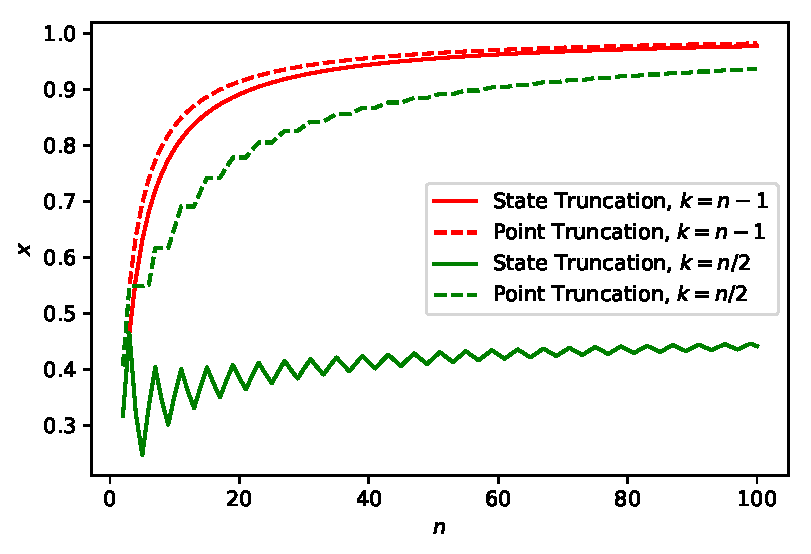
\includegraphics[width=0.45\linewidth]{classical_sim/max_x_samek}}
\hfill
\subfloat[\label{fig:max-eta-samek}]{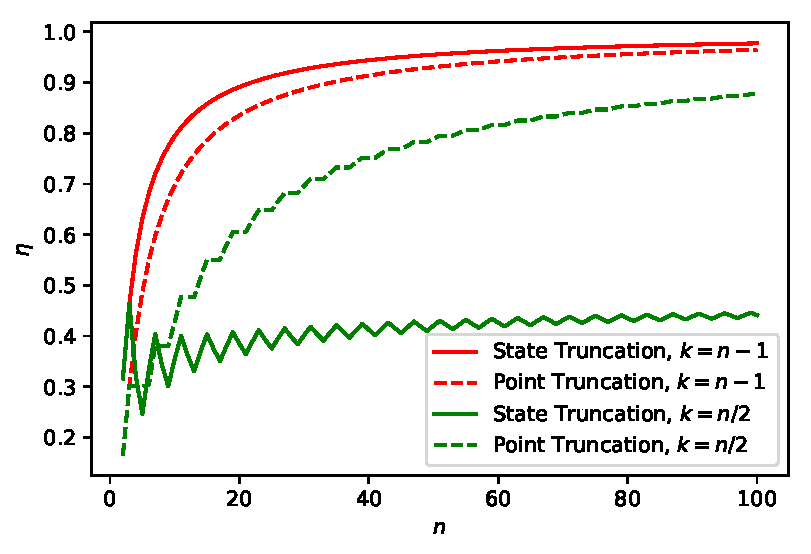
\includegraphics[width=0.45\linewidth]{classical_sim/max_eta_samek}}
\caption[Highest value of $x$ and $\eta$ simulable via state or point truncation]{\label{fig:samek} 
Highest value (\ref{fig:max-x-samek}) of $x$ when $\eta=1$ and (\ref{fig:max-eta-samek}) of $\eta$ when $x=1$ simulable via state (solid) or point (dashed) truncation up to 10\% error ($\epsilon=0.1$). 
The number of photons, $n$, is varying, with $k$ chosen as either $k=n-1$ (red) or $k=n/2$ (green).
The oscillatory behaviour is due to rounding $k=n/2$ when $n$ is odd.}
\end{figure}

We start by comparing the performance of the two algorithms when truncated at the same level $k$. 
This is of interest as in both approaches $k$ is considered to be a parameter defining the interference between photons. 
To do so, we consider the error bounds of classically simulating $n$-photon Boson Sampling for $n$ ranging between 2 and 100. 
The values chosen for $k$ depend on $n$: we consider $k=n-1$ as the upper limit of what the two algorithms can achieve without simulating the full distribution, and also $k=n/2$ as a more feasible, though still exponential time, value.

The result is plotted in Figure \ref{fig:samek}, where in (\ref{fig:max-x-samek}) we show the highest value of $x$ simulable assuming no loss ($\eta=1$) and in (\ref{fig:max-eta-samek}) we show the highest value of $\eta$ simulable assuming the photons are fully indistinguishable ($x=1$). 
For all cases, we are considering simulations up to 10\% error.

There are a number of things we can note from Figure \ref{fig:samek}. 
First is that when $k=n-1$, we can see that both algorithms tend to the same maximum values of distinguishability and loss. 
In the case of distinguishability, we can easily see why by considering the error bounds of both algorithms. 
One can see from Equation (\ref{eqn:error-sum}) that state truncation will have a simple error bound in this case of $\epsilon \leq x^n$, meaning that for constant error the largest value of $x$ simulable is $x = \epsilon^{1/n}$. 
For point truncation, recall from Section \ref{sec:renema-review} that the error is bounded as

\begin{align}
\mean[\Delta P] &\leq \frac{m^n}{n!}\sqrt{\var[\Delta P]}\\
&\leq \frac{m^n}{n!}\sqrt{\sum_{j=k+1}^nx^{2j}\var[c_j]}\\
&\leq \frac{1}{\sqrt{e}}\sqrt{\sum_{j=k+1}^nx^{2j}\sum_{l=0}^{n-j}\frac{1}{l!}}\label{eqn:renema-error-exact}.
\end{align}

Setting $k=n-1$ shows that the error is similarly bounded as $\epsilon \leq x^n/\sqrt{e}$, leading to a largest value of $x=(\epsilon\sqrt{e})^{1/n}$. 
Thus, although the highest value of $x$ simulable via point truncation is higher than that via state truncation, the difference will decrease in the limit of large $n$. 
Curiously we see the same effect as well in the case of loss, but now the highest value of $\eta$ simulable via state truncation is higher than that of point truncation. 
Again, this can be shown to hold theoretically: For state truncation the error scales as $\epsilon \leq \eta^n$ according to Equation (\ref{eqn:lossy-worst}), corresponding to $\eta=\epsilon^{1/n}$; whereas for point truncation we see from Equation (\ref{eqn:renema-error-exact}) and substituting $x=\sqrt{\eta}$ that the error scales as $\epsilon \leq \eta^{n/2}/\sqrt{e}$, meaning a maximum value of $\eta$ is $\eta=(e\epsilon^2)^{1/n}$. 
In the limit of large $n$ these differences will also tail off.

For $k=n/2$, we see that for both distinguishability and loss point truncation is more powerful than state truncation. 
Although this is harder to formally prove, there is intuition to see why this is the case. 
For state truncation, we know that for a small error to be achievable we need $k\geq n\eta x$, as this is the mean of the binomial distribution. 
Thus for $k=n/2$, we have that $\eta x \leq 1/2$, and in both cases we see the highest value of $x$ and $\eta$ tending to a value below $1/2$. 
For point truncation on the other hand, we know that the error tends to a constant value only dependent on $k$ and $\eta x^2$ in the limit of large $n$. 
As a result, it is unsurprising that for $k$ increasing linearly with $n$ the highest values of $x$ and $\eta$ will increase.


\subsection{Comparison of runtimes}
\label{subsec:runtimes}

\begin{figure}
\begin{center}
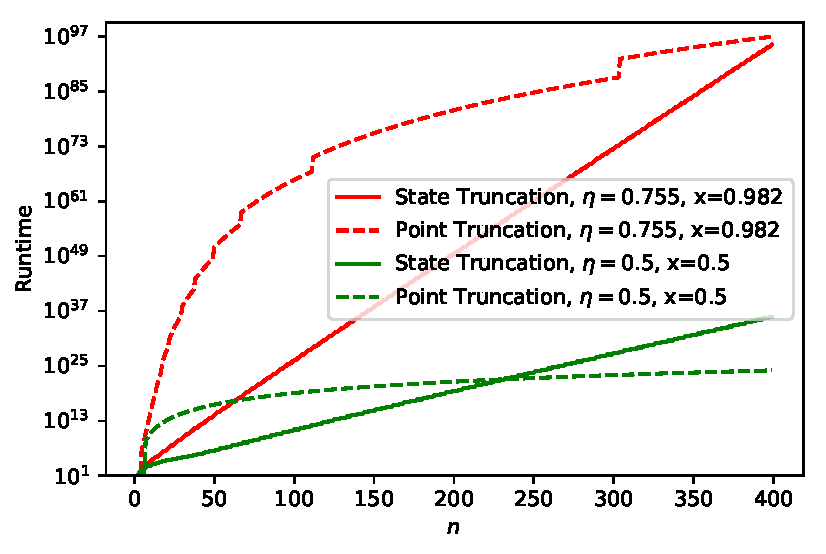
\includegraphics[width=0.5\linewidth]{classical_sim/runtime}
\end{center}
\caption[Approximate runtime to simulate $n$-photon Boson Sampling with chosen values of $\eta$ and $x$ via state or point truncation]{\label{fig:runtime} Approximate runtime (number of operations) to simulate $n$-photon Boson Sampling with chosen values of $\eta$ and $x$ up to 10\% error ($\epsilon=0.1$) via state (solid) or point (dashed) truncation. Note that a modern supercomputer running for an hour can perform roughly $10^{20}$ operations.}
\end{figure}

We next consider the runtime required to simulate $n$-photon Boson Sampling up to 10\% error via either method. 
The motivation for this comparison is that the runtime of the two algorithms at the same value of $k$ are significantly different. 
In particular, the runtime of state truncation is only dependent on $k$ and not $n$, whereas the runtime for point truncation depends on a scaling of approximately $O(n^{2k})$.

To understand how the runtimes scale, in Figure \ref{fig:runtime} we plot the runtimes of classically simulating $n$-photon Boson Sampling experiments via the two approaches for fixed values of $\eta$ and $x$. 
The values of $k$ chosen for each algorithm are the smallest values for an error of at most 10\%. 
For choosing $\eta$ and $x$, we give two example cases. 
The first (Figure \ref{fig:runtime}, red), where $\eta=0.755$ and $x=0.982$, is an example of a hypothetical best experiment we could build with current technology, with the most lossless sources (82\%) \cite{slussarenko2017}, interferometers (99\%) \cite{wang2018} and detectors (93\%) \cite{marsili2013}, and the highest level of photon indistinguishability (98\%) \cite{ornelashuerta2020}. 
The second case (Figure \ref{fig:runtime}, green), where $\eta=x=0.5$, is an example of how the two algorithms perform in what would be considered a poor experiment for both distinguishability and loss. 
Actual Boson Sampling experiments are likely to fall between these two extremes.

In both cases, state truncation appears to outperform point truncation for near-term photon experiments, with point truncation eventually being able to perform faster for larger values of $n$. 
When $\eta=x=0.5$, point truncation performs better when $n$ is approximately larger than 230. 
In the case of $\eta=0.755, x=0.982$, point truncation doesn't perform better for any $n < 400$ photons. 
This gives an idea of the regions in which the polynomial runtime of point truncation can be better or worse than the exponential runtime of state truncation.

It is also worth noting that just because point truncation is faster than state truncation for large enough $n$ does not necessarily mean that either algorithm is efficient in these cases. 
When $\eta=x=0.5$, point truncation only becomes more efficient at instances where both algorithms already require the order of $10^{22}$ operations. 
And in the case where $\eta=0.755, x=0.982$, both algorithms have runtimes of approximately $10^{96}$ operations while still not reaching a sufficiently large $n$ for point truncation to outperform state truncation.


\subsection{Comparison at same runtime}
\label{subsec:same-runtime}

\begin{figure}
\subfloat[\label{fig:max-x-fixed-n-90}]{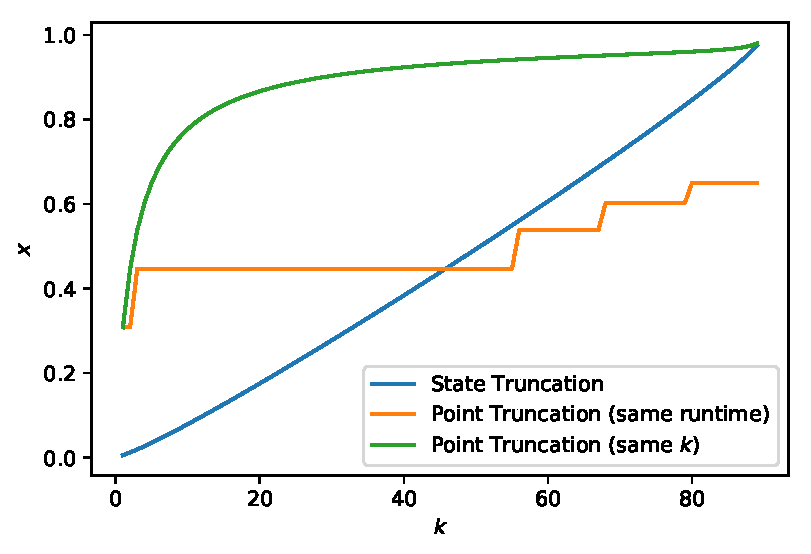
\includegraphics[width=0.45\linewidth]{classical_sim/max_x_fixed_n_90}}
\hfill
\subfloat[\label{fig:max-eta-fixed-n-90}]{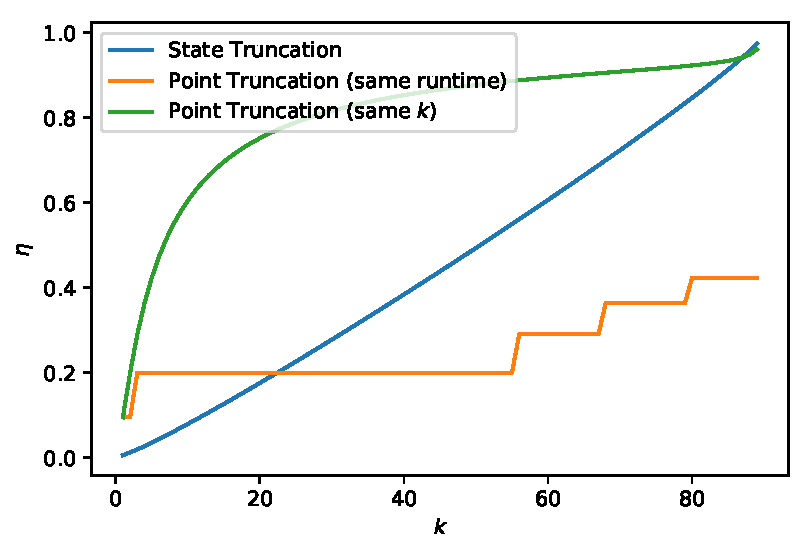
\includegraphics[width=0.45\linewidth]{classical_sim/max_eta_fixed_n_90}}
\caption[Highest value of $x$ and $\eta=1$ simulable for 90-photon boson sampling at truncation level $k$]{\label{fig:fixed-n-90} 
Highest value (\ref{fig:max-x-fixed-n-90}) of $x$ when $\eta=1$ and (\ref{fig:max-eta-fixed-n-90}) of $\eta$ when $x=1$ simulable for 90-photon boson sampling at truncation level $k$ up to 10\% error ($\epsilon=0.1$). 
Blue line indicates highest values simulable via state truncation at level $k$, green lines indicate highest values simulable via point truncation at level $k$, orange lines indicate highest values simulable by point truncation at level $k'$ such that $k'$ is the smallest level of truncation such that the approximate runtime of point truncation at level $k'$ is longer than the runtime of state truncation at level $k$.}
\end{figure}

Now we consider both truncation level and runtime, and compare the algorithms when restricted to comparable runtimes. 
To do this, we shall consider the challenge of simulating a 90-photon Boson Sampling experiment, and the largest values of distinguishability and loss that can be simulated at level $k$ with 10\% error. 
The motivation for this is that $90$ photons has been suggested as strict upper bound for what is achievable using classical computation~\cite{dalzell2018}. 

The results are shown in Figure \ref{fig:fixed-n-90}, detailing for each algorithm the highest value of $x$ simulable when $\eta=1$ (\ref{fig:max-x-fixed-n-90}) and the highest value of $\eta$ simulable when $x=1$ (\ref{fig:max-eta-fixed-n-90}). 
In both figures, the blue line indicates state truncation at level $k$, and the green line indicates point truncation at level $k$. 
However, the runtime of state truncation at level $k$ and point truncation at level $k$ are likely to be drastically different. 
To take runtime into consideration as well, we consider the orange line which indicates point truncation at level $k'$, where $k'$ is the smallest integer such that the approximated runtime of point truncation at level $k'$ is longer than that of state truncation at level $k$. 
This allows us to compare the performance of the two algorithms when restricted to similar runtimes.

Considering distinguishability in Figure \ref{fig:max-x-fixed-n-90}, we can note that point truncation with comparable runtime performs better up to $k\leq 45$, after which the methods are roughly comparable with state truncation performing marginally better, before becoming more dominant for $k\geq 60$. 
It has been suggested that boson sampling with 50 indistinguishable photons is roughly the limit of what can be classically simulated on a supercomputer \cite{neville2017, clifford2017, zhang2018}, so it appears that when considering distinguishability, the algorithms are roughly comparable in this case.

When considering loss in Figure \ref{fig:max-eta-fixed-n-90}, we see a noticeable improvement for state truncation. 
Now point truncation under the same runtime only performs better up to $k\leq 22$, with state truncation performing considerably better for higher values of $k$. 
Boson Sampling with up to 30 indistinguishable photons is already known to be classically simulable on a standard laptop \cite{neville2017}, so this appears to offer a noticeable improvement even for fast classical simulations.



\section{Non-uniform loss}

We finish by briefly considering non-uniform loss, where each photon survives a lossy optical component with probability $\tau$. 
This model of loss has been considered before \cite{garciapatron2017,oszmaniec2018}, but without the incorporation of distinguishability. We can do this using the same methods as other non-uniform loss results, by extracting non-uniform losses into a layer of uniform losses followed by a lossy interferometer. 
The uniform loss layer means that each photon has probability $\eta=\tau^s$ of surviving, where $\tau$ is the loss of each optical component and $s$ is the smallest number of lossy optical components a photon interacts with. 
If we take the total number of lossy components to be $d$, the remaining lossy circuit can be modelled as an $(m+d)$-mode interferometer, with lost photons ending up in the additional $d$ modes. 
Thus we can achieve the same error as Equation (\ref{eqn:lossy-worst}) in $O(k2^k+\poly(k,m,d))$ time. 
In typical schemes for linear interferometers, $d$ is at most polynomial in $m$ \cite{reck1994,clements2016}, so the overhead from these additional modes is small. 
We can bound the error to a decreasing value in terms of $n$ if $k>nx\tau^s$. Taking the logarithm on both sides and rearranging for $s$, we find that this holds if

\begin{equation}
s>\frac{\log n-\log 1/x-\log k}{\log1/\tau}.
\end{equation}

This matches results in \cite{garciapatron2017,oszmaniec2018}, showing that boson sampling can be classically simulated if each photon encounters at least a logarithmic number of lossy components. 
It also shows how distinguishability can affect the simulability of lossy components in Boson Sampling: if our photons are more distinguishable, corresponding to a smaller value of $x$, then we can simulate shallower (i.e.\ less total loss) optical circuits.

\section{Discussion of possible improvements}
\label{sec:small-photon-no}

There are several possible ways one might seek to improve this research. In this section we shall give two potential improvements, and discuss their potential. Although we do not provide full analysis for general $n$, we can look at cases where there are a small number of photons and use this as a springboard for discussing how these improvements might work for general $n$.

\subsection{Computing the exact trace distance}
\label{ssec:exact-trace-distance}

\begin{figure}
\subfloat[\label{fig:2-photon-trace}]{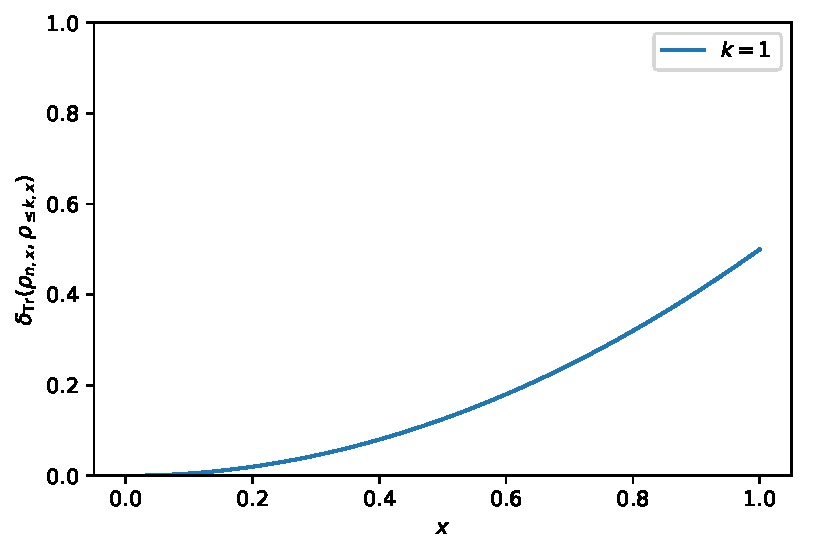
\includegraphics[width=0.45\linewidth]{classical_sim/2_photon_trace}}
\hfill
\subfloat[\label{fig:3-photon-trace}]{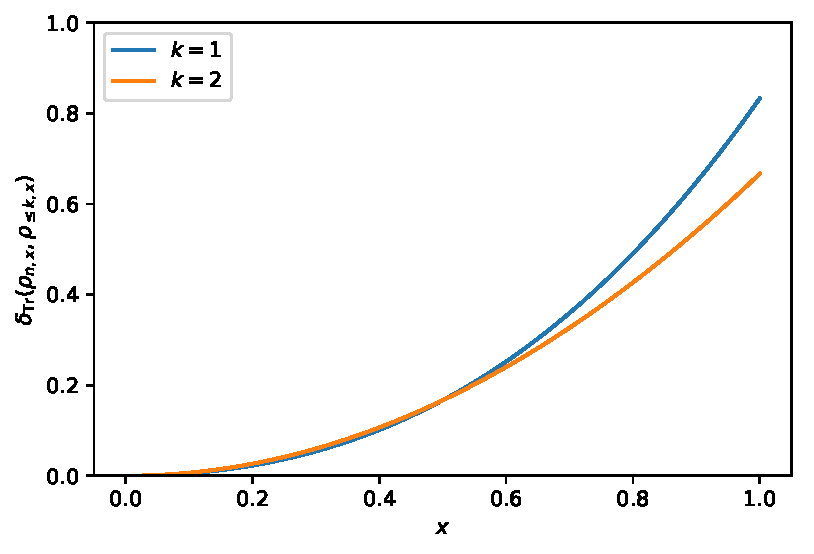
\includegraphics[width=0.45\linewidth]{classical_sim/3_photon_trace}}

\subfloat[\label{fig:4-photon-trace}]{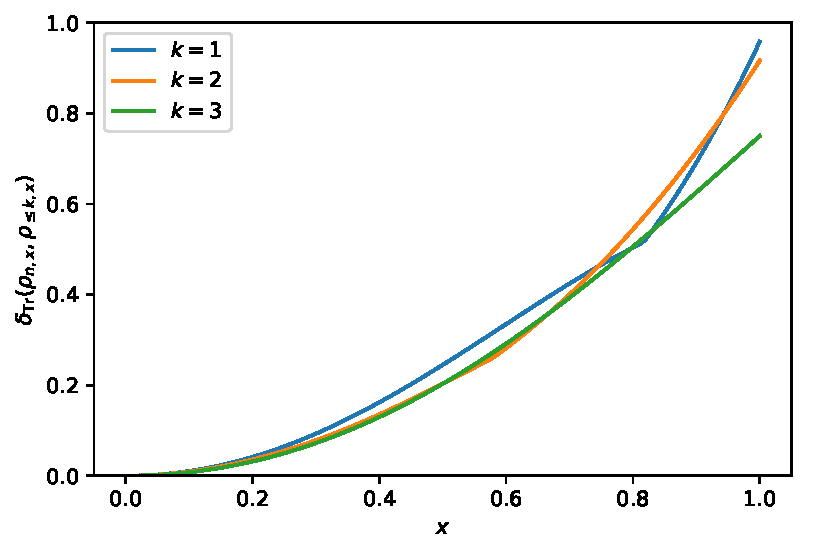
\includegraphics[width=0.45\linewidth]{classical_sim/4_photon_trace}}
\hfill
\subfloat[\label{fig:5-photon-trace}]{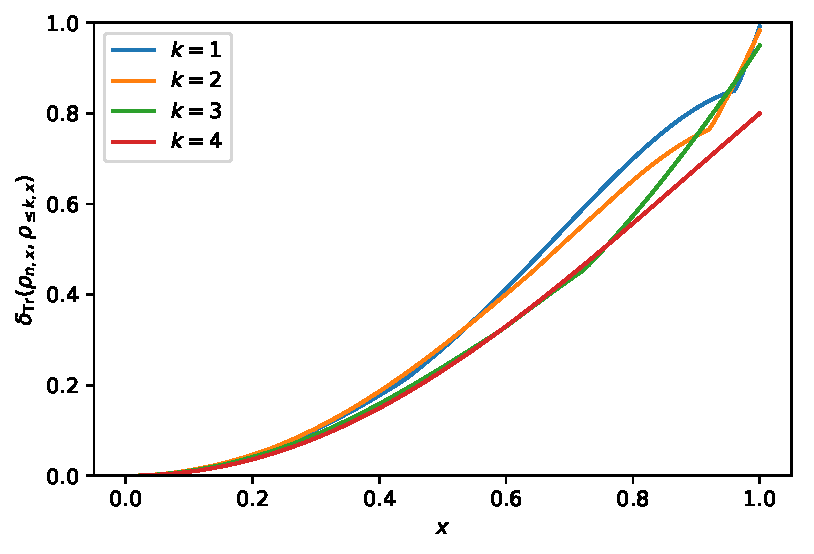
\includegraphics[width=0.45\linewidth]{classical_sim/5_photon_trace}}

\subfloat[\label{fig:6-photon-trace}]{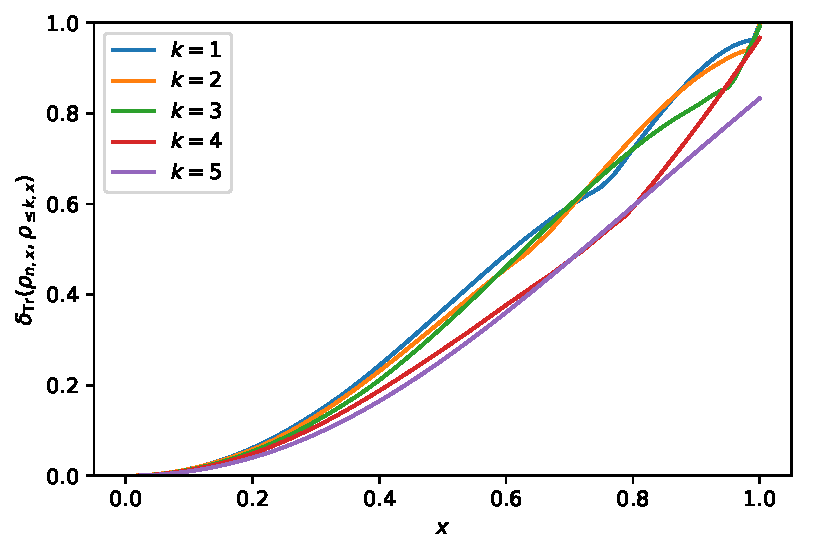
\includegraphics[width=0.45\linewidth]{classical_sim/6_photon_trace}}
\hfill
\subfloat[\label{fig:7-photon-trace}]{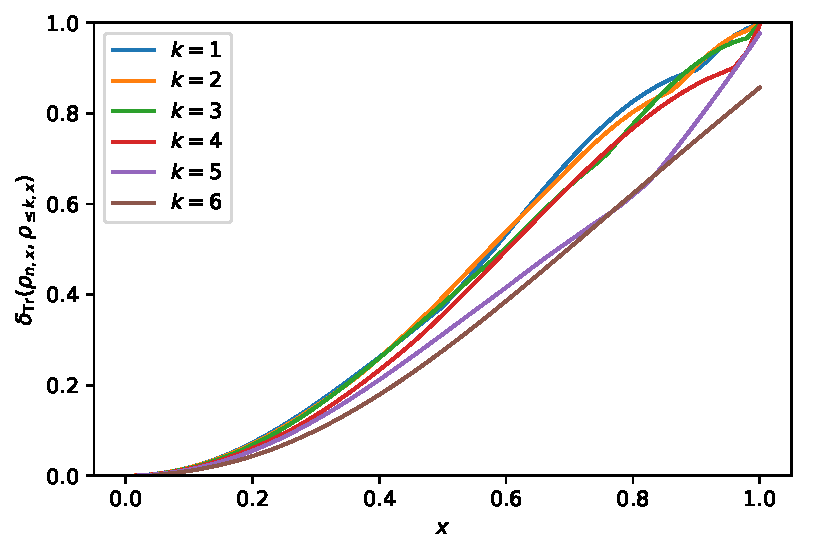
\includegraphics[width=0.45\linewidth]{classical_sim/7_photon_trace}}
\caption[Exact trace distance between $\rho_{n,x}$ and $\rho_{\leq k, x}$ over $x$ for $k< n, n=2,\dots,7$]{\label{fig:exact-trace} 
Exact trace distance betweem $\rho_{n,x}$ and $\rho_{\leq k, x}$ over $x$ for all $k < n$ for (\ref{fig:2-photon-trace}) $n=2$, (\ref{fig:3-photon-trace}) $n=3$, (\ref{fig:4-photon-trace}) $n=4$, (\ref{fig:5-photon-trace}) $n=5$, (\ref{fig:6-photon-trace}) $n=6$ and (\ref{fig:7-photon-trace}) $n=7$.}
\end{figure}

In our analysis of the worst-case error bounds, we have simply used the property of the trace distance being convex. However, this is only an upper bound, and it could be that the actual trace distance is lower. How much can we improve this bound by more direct calculation?

Sadly there is not an easy way of calculating the exact trace distance, as we have managed to do for the fixed distinguishability cases in Section \ref{ssec:fixed-dist-distance}. In lieu of this, we use analytical code to compute the trace distance for small numbers of photons. Using symbolic programming in Mathematica, we are able to compute the exact trace distance in terms of $x$ for varying $k$ and up to four photons. Furthermore, we can use analytical programming in Matlab to produce figures plotting the trace distance over $x$ for varying values of $k$ and up to seven photons.

\begin{table}
\begin{center}
\begin{tabularx}{\textwidth}{|C|p{4cm}|p{4cm}|p{4cm}|}
\hline  & \multicolumn{3}{|c|}{$k$} \\
\hline $n$ & 1 & 2 & 3 \\
\hline 2 & $x^2/2$ &  &  \\
\hline 3 & $x^2(3+2x)/6$ & $2x^2/3$ &  \\
\hline 4 & $x^2(30+16x-9x^2+9|2-3x^2|)/48$ & $x^2(18+4x-6x^2+3|1-3x^2|+|1-4x+3x^2|)/24$ & $x^2(3+x-x^2)/4$\\\hline
\end{tabularx}
\end{center}
\caption[Exact equations for $\tdist(\rho_{n,x}, \rho{\leq k, x})$ for $k < n, n=2,\dots,4$]{Exact equations for $\tdist(\rho_{n,x}, \rho_{\leq k, x})$ for $k < n$ and $n=2,3,4$.}
\label{tab:exact-trace}
\end{table}

The formulae computed via Mathematica are given in Table \ref{tab:exact-trace}, and the results from Matlab computation are given in Figure \ref{fig:exact-trace}, with each subfigure showing the trace distance for varying $n$ and $k$. It is very challenging to discern a general pattern here, unlike the fixed distinguishability cases discuseed in Section \ref{ssec:fixed-dist-distance}; the formulae produced by Mathematica start looking complicated even for $n=4$. Larger values of $n$ were attempted in both Matlab and Mathematica, but had to be abandoned due to computation time.

We can see that for high values of $x$ all of these approximations start to fail. Part of the reason for this is how few photons we have; if on average we expect $nx$ photons then for a good approximation with $k<n$ we would expect that $x<(n-1)/n$, which will be fairly low with these small values of $n$.

It is interesting to note from Figure \ref{fig:exact-trace} that for some values of $x$ there are some values of $k$ where $\tdist(\rho_{n,x},\rho_{\leq k, x}) < \tdist(\rho_{n,x},\rho_{\leq k+1, x})$. This is very surprising; we would expect that the trace distance would decrease for all $x$ as $k$ increases, as this would correspond to more indistinguishable photons. We do not know why this is and leave it as an open question for future research. It is however worth emphasising in these cases that the trace distance is an upper bound, and it might be that in practice interferometers which achieve this perfect maximisation of trace distance do not exist. We again leave this as a direction for future research, but note that this is similar to the question explored by Stanisic and Turner, who looked at this in the fixed distinguishability case \cite{stanisic2018}.

\subsection{Expanding in terms of representations}
\label{ssec:irrep-expansion}

Another natural question is if we can instead expand in terms of representations rather than in terms of state. This would provide us with an alternative decomposition where rather than needing to sample which photons are indistinguishable, we would instead be sampling which immanants we need to compute to find the probability of an outcome. It is hard to analytically work out how the different immanants contribute for general $n$, but in this section we will use results noted by Stanisic and Turner \cite{stanisic2018} to show the decompositions for two and three particles, as well as offer some general comments on why this technique might not necessarily provide a better classical simulation but could still be of theoretical interest.

We shall start with the simpler case of two photons, which we shall assume to be in the first two spatial modes. As noted earlier, the state takes the form

\begin{equation}
\rho_x = x^2\rho_{\{1,2\}} + x(1-x)(\rho_{\{1\}} + \rho_{\{2\}}) + (1-x)^2\rho_{\emptyset},
\end{equation}

\noindent where $\rho_I$ is the state corresponding to photons in modes $I\subseteq\{1,2\}$ being indistinguishable. The state corresponding to the fully indistinguishable case is fully symmetric, giving us

\begin{equation}
\rho_{\{1,2\}} = \ket{\young(12)}\bra{\young(12)},
\end{equation}

\noindent where we have suppressed notation for the irrep as it is implied by the Young tableaux, and we have suppressed the Symmetric irrep basis as it is one dimensional in the two particle cases. Note that states where only one photon is in the indistinguishable set are effectively fully distinguishable as well. As a result, the states $\rho_{\{1\}}, \rho_{\{2\}}$ are equal to $\rho_{\emptyset}$, the fully distinguishable state, which as described in the irrep basis in Equation \ref{distinguishable-irreps} gives us

\begin{equation}
\rho_\emptyset = \frac{1}{2}\left(\ket{\young(12)}\bra{\young(12)}+\left|\young(1,2)\right\rangle\left\langle\young(1,2)\right|\right).
\end{equation}

The overall state can therefore be written as

\begin{align}
\rho_x &= x^2\ket{\young(12)}\bra{\young(12)} + \frac{(2x(1-x)+(1-x)^2)}{2}\left(\ket{\young(12)}\bra{\young(12)}+\left|\young(1,2)\right\rangle\left\langle\young(1,2)\right|\right)\\
&= \frac{1}{2}\left((2x^2 + 2x(1-x)+(1-x)^2)\ket{\young(12)}\bra{\young(12)}+(2x(1-x)+(1-x)^2)\left|\young(1,2)\right\rangle\left\langle\young(1,2)\right|\right)\\
&= \frac{1+x^2}{2}\ket{\young(12)}\bra{\young(12)}+\frac{1-x^2}{2}\left|\young(1,2)\right\rangle\left\langle\young(1,2)\right|.
\end{align}

As $x\rightarrow 1$, this tends towards only the fully symmetric irrep contributing, as expected. However, even as $x\rightarrow 0$, the fully symmetric irrep still contributes to half of the outcome probability.

We can also work out the explicit decomposition for three particles, again assuming our photons start in the first three modes. The state is now

\begin{equation}
\rho_x = x^3\rho_{\{1,2,3\}} + x^2(1-x)(\rho_{\{1,2\}}+\rho_{\{1,3\}}+\rho_{\{2,3\}}) + x(1-x)^2(\rho_{\{1\}}+\rho_{\{2\}}+\rho_{\{3\}}) + (1-x)^3\rho_\emptyset.
\end{equation}

The fully indistinguishable state is similar to before:

\begin{equation}
\rho_{\{1,2,3\}} = \ket{\young(123)}\bra{\young(123)}.
\end{equation}

Rather than writing out the full Young-Yagamouchi basis, we shall simply use a 1 or 2 subscript to denote the basis state of the $(1,2)$ irrep of the Symmetric group, which, as noted in Theorem \ref{thm:schur-weyl-duality}, induces a multiplicity on the corresponding irrep of the Unitary group. This matches the notation used in Stanisic and Turner \cite{stanisic2018}. With this in mind, the uniform mixture of all three singly distinguishable states is

\begin{align}
\rho_{\{1,2\}}+\rho_{\{1,3\}}+\rho_{\{2,3\}} &= \ket{\young(123)}\bra{\young(123)} + \frac{1}{2}\left(\left|\young(12,3)_1\right\rangle\left\langle\young(12,3)_1\right| + \left|\young(12,3)_2\right\rangle\left\langle\young(12,3)_2\right|\right)\nonumber\\
&\quad+ \frac{1}{2}\left(\left|\young(13,2)_1\right\rangle\left\langle\young(13,2)_1\right| + \left|\young(13,2)_2\right\rangle\left\langle\young(13,2)_2\right|\right).
\end{align}

Finally, we note that the fully distinguishable states $\rho_{\emptyset}, \rho_{\{1\}}, \rho_{\{2\}}, \rho_{\{3\}}$ can all be written as

\begin{align}
\rho_\emptyset &= \frac{1}{6}\left(\ket{\young(123)}\bra{\young(123)} + \left|\young(12,3)_1\right\rangle\left\langle\young(12,3)_1\right| + \left|\young(12,3)_2\right\rangle\left\langle\young(12,3)_2\right|\right)\nonumber\\
&\quad+\frac{1}{6}\left(\left|\young(13,2)_1\right\rangle\left\langle\young(13,2)_1\right| + \left|\young(13,2)_2\right\rangle\left\langle\young(13,2)_2\right| + \left|\young(1,2,3)\right\rangle\left\langle\young(1,2,3)\right|\right).
\end{align}

The overall state can be expanded as

\begin{align}
\rho_x &= \frac{1}{6}\left((1+3x^2+2x^3)\ket{\young(123)}\bra{\young(123)}\right)\nonumber\\
&\quad+\frac{1}{6}\left((1-x^3)\left(\left|\young(12,3)_1\right\rangle\left\langle\young(12,3)_1\right| + \left|\young(12,3)_2\right\rangle\left\langle\young(12,3)_2\right|\right)\right)\nonumber\\
&\quad+\frac{1}{6}\left((1-x^3)\left(\left|\young(13,2)_1\right\rangle\left\langle\young(13,2)_1\right| + \left|\young(13,2)_2\right\rangle\left\langle\young(13,2)_2\right|\right) + (1-3x^2+2x^3)\left|\young(1,2,3)\right\rangle\left\langle\young(1,2,3)\right|\right).
\end{align}

It is again possible to verify that as $x\rightarrow 1$ then only the symmetric irrep contributes, and as $x \rightarrow 0$ then all irreps contribute uniformly.

\begin{figure}
\subfloat[\label{fig:irreps-n-2}]{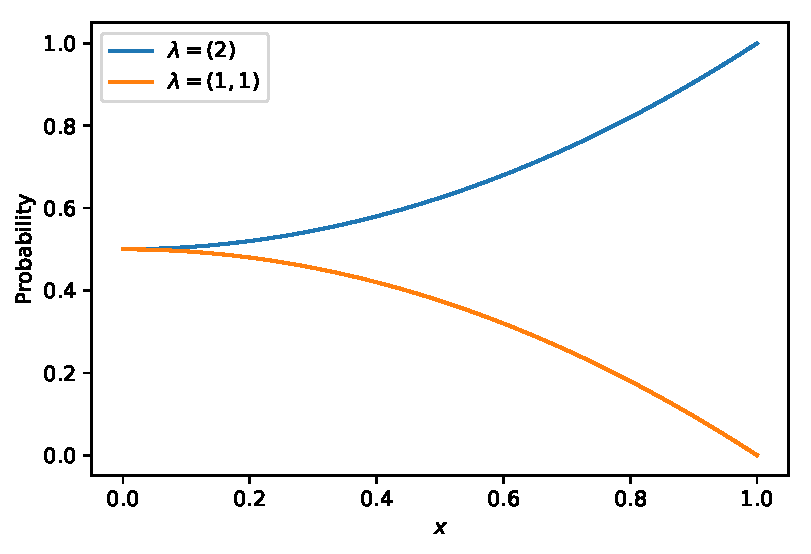
\includegraphics[width=0.45\linewidth]{classical_sim/irreps_n_2}}
\hfill
\subfloat[\label{fig:irreps-n-3}]{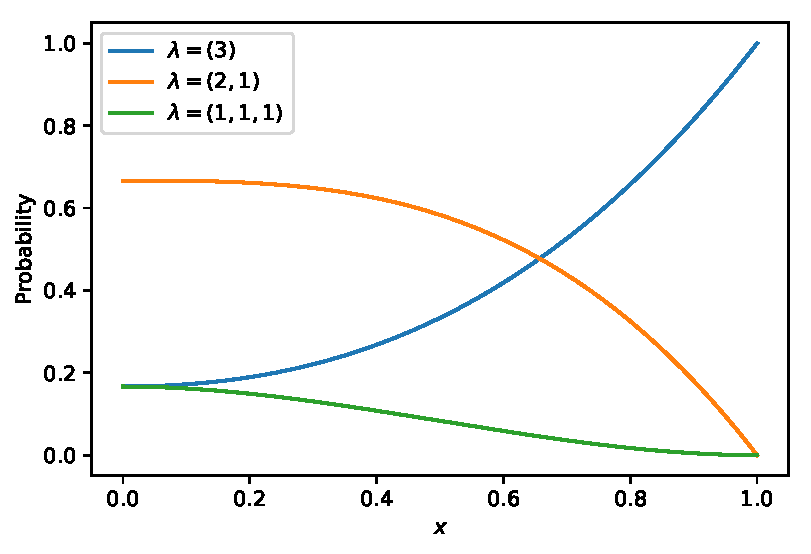
\includegraphics[width=0.45\linewidth]{classical_sim/irreps_n_3}}
\caption[Probability of different irreps when $n=2$ and $n=3$.]{\label{fig:irreps} Probability of different irreps when (\ref{fig:irreps-n-2}) $n=2$ and (\ref{fig:irreps-n-3}) $n=3$. Note that if for the $\lambda=(2,1)$ irrep in Figure \ref{fig:irreps-n-3}, we have shown the probability of sampling any of the multiplicities, when in reality this is a uniform distribution of the four multiplicities.}
\end{figure}

In Figure \ref{fig:irreps} we have plotted the probability of sampling from different irreps over $x \in [0,1]$ for (\ref{fig:irreps-n-2}) $n=2$ and (\ref{fig:irreps-n-3}) $n=3$. As already mentioned, this makes clear how at $x=0$ all terms have equal probability, and as $x\rightarrow 1$ the fully symmetric irrep begins to dominate. It is interesting to note that for $n=3$, $\lambda=(2,1)$ is the most likely irrep; this is because of the multiplicities within this irrep for both $\symm_3$ and $\unitary(3)$. By solving the cubic equation

\begin{equation}
1+3x^2+2x^3 = 4-4x^3,
\end{equation}

\noindent we find that the two overlap when $x \approx 0.657$, when both irreps have probability approximately $0.4773$ of being sampled\footnote{Note that there are other solutions to this cubic equation, but $x\approx 0.657$ is the only real-valued solution between 0 and 1 and is therefore the only solution relevant to us.}.

We now go back to the question at the start of this section, as to whether or not this could lead to another simulation. A potential method of simulation, akin to the point and state truncation methods, would be to truncate which irrep we sample from. In other words, we sample an irrep with at most $n-k$ nonzero rows for some truncation level $k$, and then perform sampling conditioned on that irrep.

There are a few limitations with this approach. The first is that this expansion is nontrivial, and we do not currently have a convenient general form for it, unlike with state truncation where we simply follow the binomial distribution. The second is that, even in the fully distinguishable case, the matrix permanent still plays a role in the distribution, so for any value of $x$ including $x=0$ we are going to have some error if we truncate before the symmetric irrep. And the third is that it is unclear how to classically simulate these irrep states under unitary action; it seems reasonable for them to be related to matrix immanants in a way similar to Tichy and M\o lmer \cite{tichy2017}, but even if so classical algorithms for computing more general immanants are less well-known, though some do exist \cite{hartmann1985, barvinok1990, burgisser2000, mertens2013}. Obviously classical algorithms for the special cases of the permanent and determinant are well-known with exponential \cite{glynn2010} and polynomial \cite{fisikopoulos2016} runtimes, respectively.

So if this decomposition does not provide us with faster classical algorithms, what might it be useful for? Well, there are some instances of $\lambda$ for which matrix imminants are known to be hard. The best-known of these is the permanent \cite{valiant1979, aaronson2011}, but other forms of immanant such as for hook or rectangular diagrams are also know to be $\sharpp$-hard \cite{burgisser2000immanants}. If one is able to construct a form of distinguishable-photon Boson Sampling such that the probability ends up being largely concentrated in these hard instances, and show that computing the sum of these immanants is at least as hard as computing a single immanant, then this could potentially lead to new proofs of hardness for Boson Sampling under distinguishability. We leave this question as future work.

\section{Conclusion}
\label{sec:conclusion}

In recent years significant improvements have been made in the ability of classical computers to simulate Boson Sampling under various imperfections. 
However, while it is of theoretical interest to demonstrate asymptotic improvements in classical simulation, the whole reason for proposals such as Boson Sampling is to offer speedups for near-term devices. 
Although our algorithm will not scale polynomially as the number of photons increases, we find that a substantial improvement over current classical algorithms can be achieved for the numbers of photons that experimentalists are currently aiming for. 
In doing so, we have effectively set a benchmark for what is required of a 50--90 photon Boson Sampling device.

\subsection{Open questions}

There are a number of ways one could improve this classical simulation. 
In particular, the approach of Ref.~\cite{renema2018} for truncation when looking at near-term devices is dependent on Metropolised Independence Sampling. 
A direct adaptation of the Clifford \& Clifford algorithm to this approach would almost certainly offer an improvement over our algorithm. 
However, such an adaptation is non-trivial, due to the fact that the terms in the expansion do not correspond to states, something that motivated our work here.

There are other open questions we would like to consider as well. The first would be to reduce the average-case error bounds to be less than our worst-case error bounds. This would most likely involve an alternative to using the triangle inequality. The second would be to find a way of explaining the difference in dependence on $\eta$ and $x$ between point and state truncation, and ideally improving either algorithm in the process.

Finally it would be interesting to extend these results to other photonics-based quantum advantage schemes, such as Gaussian Boson Sampling \cite{hamilton2017}. The probability distribution of Gaussian Boson Sampling is that of $n$ indistinguishable squeezed states at the output of an $m$-mode linear optical interferometer, and depends on the Hafnian of a matrix. Unlike Boson Sampling, there is no known polynomial time classical algorithm for computing the probability of a single outcome from $n$ fully distinguishable squeezed states. An attempt to remedy this was recently presented by Renema \cite{renema2019}, by looking at the probability of an outcome from a Gaussian Boson Sampling as a linear combination of matrix permanents and extending the point truncation method accordingly, but this result hits a stumbling block in the form of an open problem related to the hardness of matrix permanents. On the other hand, it is classically efficient to sample $n$ fully distinguishable squeezed states, via a similar approach to that used for classically sampling distinguishable single photons \cite{aaronson2014}: For each squeezed state, one first samples the number of photons in that squeezed state via the inverse binomial distribution \cite{wu2019}, then each of those photons is sampled through the interferometer individually, as photons that start in the same spatial mode do not interfere with one another and their outcomes can therefore be sampled individually. As a result, adapting the Clifford \& Clifford algorithm to non-ideal Boson Sampling models provides an important step towards being able to classically simulate imperfections in Gaussian Boson Sampling. This, combined with recent classical simulation algorithms for ideal Gaussian Boson Sampling \cite{quesada2019, wu2019}, show strong potential for these results to extent to Gaussian Boson Sampling.


\subsection{Note Added}

During this work we were made aware of independent work by V. Shchesnovich, which also shows that the model of distinguishability considered by Renema et al.\ corresponds to that of selecting indistinguishable photons via the binomial distribution \cite{shchesnovich2019}. 
This is derived using significantly different methods from those used in this manuscript, and does not consider classical simulation of distinguishability via the above method (though this has been anticipated~\cite{shchesnovich2019clifford}).
\chapter{Conclusion}
\label{chp:conclusion}

It truly is astounding to see what progress has been made in quantum computing. From the 1980s, when quantum computers were a vague concept with no theoretical benefits beyond possibly simulation \cite{feynman1982}, to the 1990s when the first theoretical speedups were discovered \cite{shor1994, grover96}, to today where demonstration devices are now readily available and showcasing the potential that quantum computers hold \cite{rigetti, ibm}. All of this culminating in Google's astonishing result: a quantum computer solving a problem significantly faster than what even the best supercomputers can accomplish \cite{arute2019}. This is a tremendous way to mark the start of a new decade in quantum computing.

And with this new decade, new goals must be sets. Now that we have quantum computers solving a problem faster than what is classically possible, we need to show that quantum computers can do so for a problem that is beneficial to us. And just as importantly, we need to show that quantum computers can solve this problem well.

In this thesis, we have strived to close the gap between what problems quantum computers can solve and the limitations of their architecture. In Part \ref{prt:application}, we have given a new example problem which quantum computers can offer a speedup for over the best classical algorithms: The Travelling Salesman Problem. As an NP-Hard problem with many applications, this demonstrates how quantum computers can offer speedups for even some of the most challenging problems we encounter in Computer Science and Mathematics. In Part \ref{prt:architecture}, we assess how photon distinguishability and loss affect the near-term quantum advantage architecture of Boson Sampling. In doing so, we devise new methods for mathematically modelling these imperfections via the first quantisation, and from there adapt the classical Clifford \& Clifford algorithm \cite{clifford2017} to take advantage of these issues. This emphasises how much these imperfections reduce any benefit we are likely to see, and how much effort we must do to overcome these experimental challenges in the near future.

\section{Open Questions}
\label{sec:oq}

But alas, the gap between these directions still exists, and there is yet more work to be done. We shall conclude this thesis with some open questions, such that an inspired reader might choose to pursue these routes even deeper. As we have done so throughout this thesis, we shall consider the two approaches separately.

\subsection{Applications direction}

Several open directions have already been mentioned in Section \ref{sec:tsp-conclusion}. Of particular note is the question of what other classical algorithms for the Travelling Salesman Problem can be sped up by a quantum computer. Promising directions include cut-and-count \cite{bjorklund14,bodlaender15,cygan11}, which use a combination of Monte Carlo algorithms and dynamic programming, and branch-and-bound \& branch-and-cut \cite{little1963, padberg1991, applegate2006}, for which quantum speedups already exist but most complexity understanding is empirical rather than analytical.

The fact that such speedups exist for the Travelling Salesman Problem suggests that polynomial speedups also exist for other NP-Hard problems as well. Already several other problems have seen speedups: Campbell, Khurana and Montanaro \cite{campbell2019} showed how the backtracking framework can also be applied to Boolean Satisfiability and Graph Colouring, and Montanaro \cite{montanaro2019} used the quantum speedup for branch-and-bound algorithms to find the exact ground state of Sherrington-Kirkpatrick Hamiltonians. Due to the same families of algorithms, such as dynamic programming or backtracking, being used to solve many different NP-Hard problems, it is likely that in the future we shall see polynomial speedups for many more.

But of course, this still does not address the main stumbling block when moving from these eventual speedups to a near-term speedup: That the quantum algorithm needs to run on near-term quantum computers. As noted in Campbell, Khurana and Montanaro \cite{campbell2019} and mentioned in Section \ref{sec:error-correction}, this already rules out many of these algorithms, for which the significant dependence on error correction and fault tolerance, and the classical computational overhead the comes with it, reduces any quantum speedup in practice to nought. To overcome this, we need to see these algorithms adapted to architectures which might be realisable in the near future.

We already hint at this open direction in Section \ref{sec:error-correction}, when discussing the recent work on algorithms which use classical processing to break the problem down until it is of a size that a quantum algorithm with a small number of qubits can be used \cite{dunjko2018, ge2019}. It is likely that other quantum algorithms for these problems can also be adapted to a hybrid quantum-classical framework of this form. One that we think is particularly promising is the approach of Ambainis et al.~\cite{ambainis2018}, where a polynomial speedup for dynamic programming is obtained by using a classical computation to preprocess simple spaces of the problem, followed by using Quantum Minimum Finding to search over the larger spaces. It might be possible to adapt this architecture to quantum computers with constrained amounts of memory, by more careful analysis of the quantum algorithm's memory usage and new consideration of how to partition the quantum and classical aspects of the algorithm. It is worth noting that this approach still depends on universal fault-tolerant quantum computation, but the hope is that the smaller number of logical qubits required would lead to a more feasible speedup.

There are also other near-term architectures that can be considered. Of particular note is the Quantum Adiabatic Optimisation Algorithm. When originally proposed by Farhi et al.~\cite{farhi2014}, it was used as a quantum algorithm for finding an approximation to the Max-Cut problem, which is known to be NP-Hard \cite{karp1972}. As a model of universal quantum computation \cite{lloyd2018, morales2019}, it is likely that other applications for QAOA to NP-Hard problems will also be found in the future, though it is less clear how promising a speedup QAOA will offer. Other intermediate-scale, or NISQ, devices also show potential in different applications, such as the Variational Quantum Eigensolver for simulating physical systems \cite{peruzzo2014, preskill2018}.

\subsection{Architecture direction}

There are many directions we can go when looking at near-term quantum architectures. As mentioned at the end of Chapters \ref{chp:noisy_circuit} and \ref{chp:classical_sim}, the most natural direction for continuing this work is to better understand the computational complexity of Boson Sampling under these imperfections. We have already discussed several examples of classical simulation approaches, such as \cite{renema2018, renema2018loss, garciapatron2017, oszmaniec2018, brod2019}, and have hinted at how one might prove hardness, via the computational complexity of immanants \cite{hartmann1985, barvinok1990, burgisser2000, burgisser2000immanants, mertens2013}. Better understanding of how the Quantum Schur Transform acts on certain states would also assist in this goal.

But Boson Sampling is only one of many photonic quantum computing architectures. Another interesting question is whether or not these same imperfections can be applied to variants of Boson Sampling. Many of these simulation algorithms, including our own described in Chapter \ref{chp:classical_sim}, can be naturally extended to Scattershot Boson Sampling, by simply choosing which modes our photons start in from the $\binom{m}{n}$ uniform distribution at the start. But what about Gaussian Boson Sampling? Already there have been some promising results by expanding some of the classical algorithms for vanilla Boson Sampling \cite{qi2019, quesada2019, wu2019, renema2019}, and it would be exciting to see the same for other classical algorithms. It would also be interesting to see if these algorithms could be extended to universal quantum photonic architectures, through simulating postselected, adaptive or measurement-based schemes \cite{knill2001, gimenosegovia2015}.

More broadly, we still need to work hard to find applications for Boson Sampling and its variants. As has already been mentioned, a number of promising directions exist, particularly for more general linear optics \cite{sparrow2018} and Gaussian Boson Sampling \cite{huh2015, bradler2018, schuld2019}. It will be interesting to see what other applications exist, and especially if these applications extend to other schemes.

And beyond linear optics, we need to look at the many quantum advantage proposals that have been proposed over the last several years, to see what extent we can classically simulate them as well as what applications they might have. Boson Sampling has received a lot of attention on this end, as already shown. Less is currently known about the extent to which IQP circuits and Random Circuit Sampling can be classically simulated. But there are some promising results in these directions. For IQP circuits, Bremner, Montanaro and Shepherd showed how polarisation error can lead to an efficient classical simulation, as well as how simple forms of error correction can mitigate these issues \cite{bremner2017}. As for Random Circuit Sampling, Pednault et al.~\cite{pednault2019} give an estimate for what is likely to be the largest classical simulation we can achieve, and Morimae, Takeuchi and Tani \cite{morimae2019google} suggest a classical simulator which takes advantage of the poor fidelity. Another relevant direction, considered by Bravyi et al.~\cite{bravyi2019}, looks at how much we can classically simulate random quantum circuits when there are only a small number of non-Clifford gates\footnote{Note that quantum circuits composed entirely of Clifford gates are efficiently classically simulable, and the inclusion of non-Clifford gates such as the $T$ or Toffoli gates is sufficient for universal quantum computation.}, showing that circuits with 40--50 qubits and over 60 non-Clifford gates can be simulated on a standard computer.

\section{The future}

So what lies ahead for the world of quantum computing then? It is always hard to predict what will happen, but the current state of quantum computers offer a lot of promise and potential. Google's paper has proven that potentially relevant and significant quantum devices could be realisable within our lifetime, if not already here. But in order to truly demonstrate that these devices are worth the hype and effort behind them, now is more important than ever that we push for improving the architecture to as good a quality as possible, as well as refining the problems we are proposing for them to make them more physically realisable.

Eventually, we hope that these two paths will intersect, and we will have a useful application for a quantum computer. Then, dear reader, we will have found our quantum speedup.


% =============================================================================

% Finally, after the main matter, the back matter is specified.  This is
% typically populated with just the bibliography.  LaTeX deals with these
% in one of two ways, namely
%
% - inline, which roughly means the author specifies entries using the 
%   \bibitem macro and typesets them manually, or
% - using BiBTeX, which means entries are contained in a separate file
%   (which is essentially a databased) then inported; this is the 
%   approach used below, with the databased being thesis.bib.
%
% Either way, the each entry has a key (or identifier) which can be used
% in the main matter to cite it, e.g., \cite{X}, \cite[Chapter 2}{Y}.

\backmatter

\bibliography{introduction/introduction, preliminary_q_c/preliminary_q_c, preliminary_bs/preliminary_bs, tsp/tsp, noisy_circuit/noisy_circuit, classical_sim/classical_sim}

% -----------------------------------------------------------------------------

% The thesis concludes with a set of (optional) appendicies; these are 
% the same as chapters in a sense, but once signaled as being appendicies via
% the associated macro, LaTeX manages them appropriatly.

\appendix

% =============================================================================

\end{document}
